\documentclass[11pt,a4paper,oneside]{book}

% ---------- Fonts & encoding ----------
\usepackage[T1]{fontenc}
\usepackage[utf8]{inputenc}
\usepackage{lmodern}
\usepackage{microtype}

% ---------- Layout ----------
\usepackage[a4paper,margin=2.5cm,headheight=14pt]{geometry}
\setlength{\parindent}{0pt}
\setlength{\parskip}{0.55em}

% ---------- Math, tables, graphics ----------
\usepackage{amsmath,amssymb,mathtools}
\usepackage{booktabs,tabularx,multirow,makecell,longtable,array,colortbl}
\usepackage{graphicx}
\graphicspath{{../figures/}}
\usepackage{tikz}
\usetikzlibrary{arrows.meta,positioning,shapes.geometric,calc,fit,decorations.pathreplacing,shadows}
\usepackage{textcomp}
\providecommand{\euro}{\texteuro}
\usepackage{pgfplots}
\pgfplotsset{compat=1.17}
\usepackage{enumitem}
\setlist{itemsep=0.15em,topsep=0.3em}
\usepackage{float}
\usepackage{needspace}
\usepackage{caption}
\captionsetup{font=small,labelfont=bf}

% ---------- Colours ----------
\usepackage{xcolor}
\definecolor{navy}{RGB}{20,30,120}
\definecolor{bocconi}{RGB}{50,50,160}
\definecolor{keyred}{RGB}{190,30,30}
\definecolor{addgreen}{RGB}{20,110,60}
\definecolor{lightgrey}{RGB}{242,242,242}
\definecolor{boxblue}{RGB}{230,236,250}
\definecolor{trapbg}{RGB}{253,236,236}
\definecolor{addbg}{RGB}{233,246,238}

% ---------- Headings ----------
\usepackage{titlesec}
\titleformat{\chapter}[display]{\normalfont\huge\bfseries\color{navy}}{\chaptertitlename\ \thechapter}{18pt}{\Huge}
\titleformat{\section}{\normalfont\Large\bfseries\color{navy}}{\thesection}{1em}{}
\titleformat{\subsection}{\normalfont\large\bfseries\color{navy}}{\thesubsection}{1em}{}
\titleformat{\subsubsection}{\normalfont\normalsize\bfseries\color{navy!80!black}}{}{0em}{}
\setcounter{secnumdepth}{2}
\setcounter{tocdepth}{1}

% ---------- Header / footer ----------
\usepackage{fancyhdr}
\pagestyle{fancy}
\fancyhf{}
\renewcommand{\chaptermark}[1]{\markboth{\thechapter.\ #1}{}}
\fancyhead[L]{\small\itshape Corporate Finance -- Exam Guide}
\fancyhead[R]{\small\itshape\nouppercase{\leftmark}}
\fancyfoot[C]{\thepage}
\renewcommand{\headrulewidth}{0.4pt}
\fancypagestyle{plain}{\fancyhf{}\fancyfoot[C]{\thepage}\renewcommand{\headrulewidth}{0pt}}

% ---------- Boxes ----------
\usepackage[most]{tcolorbox}
\tcbset{enhanced,breakable,boxrule=0.6pt,arc=2pt,left=6pt,right=6pt,top=4pt,bottom=4pt,fonttitle=\bfseries\small}
% key formula / key result
\newtcolorbox{keybox}[1][Key formula]{colback=boxblue,colframe=navy,title={#1}}
% definition
\newtcolorbox{defbox}[1][Definition]{colback=lightgrey,colframe=black!60,title={#1}}
% added explanation (not on slides)
\newtcolorbox{addbox}[1][Added explanation]{colback=addbg,colframe=addgreen,title={#1 \hfill\normalfont\itshape not on slides}}
% exam trap
\newtcolorbox{trapbox}[1][Exam trap]{colback=trapbg,colframe=keyred,title={#1}}
% worked example
\newtcolorbox{exbox}[1][Worked example]{colback=white,colframe=bocconi,title={#1}}

% layer tag (CORE/PRO/TECH/PRACTICE as on slides)
\newcommand{\layer}[1]{\hfill{\normalfont\footnotesize\fboxsep=1.5pt\colorbox{navy}{\textcolor{white}{\textbf{#1}}}}}
\newcommand{\added}{\textcolor{addgreen}{\textit{(added explanation)}}\ }
\newcommand{\slidefig}[1]{\par\smallskip{\footnotesize\itshape\textcolor{black!60}{#1}}\par}

% ---------- Hyperlinks ----------
\usepackage[colorlinks=true,linkcolor=navy,urlcolor=navy,citecolor=navy]{hyperref}
\usepackage{bookmark}
\usepackage{tocloft}
\setlength{\cftbeforechapskip}{4pt}
\setlength{\cftbeforesecskip}{0pt}
\renewcommand{\cftsecfont}{\small}
\renewcommand{\cftsecpagefont}{\small}
\renewcommand{\cftchapfont}{\bfseries\color{navy}}

\begin{document}

% ================= TITLE =================
\begin{titlepage}
\centering
\vspace*{5cm}
{\color{navy}\Huge\bfseries 20127 Corporate Finance\\[4pt] (Business Valuation)\par}
\vspace{1cm}
{\Large Final Exam Study Guide\par}
\vspace{0.4cm}
{\large Lectures, Discussion Questions, Formula Sheets and Exam Traps\par}
\vspace{1.5cm}
{\large MSc Finance -- Bocconi University\par}
{\large Prof.\ Stefano Rossi\par}
\vspace{1.2cm}
{\large\itshape Brought to you by Adriano La Ragione\par}
\vfill
{\small Parts One and Two -- Lectures 01--12\par}
\end{titlepage}

\thispagestyle{empty}
\vspace*{2cm}
\begin{center}
\itshape Closed-book exam, multiple choice only (1 correct answer out of 4, no penalty for wrong answers).\\[4pt]
Attending: 15 MCQ in 45 minutes (7 Part One + 7 Part Two + 1 Testimonial).\\
Non-attending: 31 MCQ in 60 minutes (14 Part One + 14 Part Two + 3 Academic Readings).\\[4pt]
No formula sheet. Basic scientific calculator only (no storage, no NPV functions).\\[14pt]
\upshape
\begin{tabular}{@{}ll@{}}
\fcolorbox{navy}{boxblue}{\rule{0pt}{6pt}\rule{6pt}{0pt}} & Key formula / key result (blue)\\
\fcolorbox{black!60}{lightgrey}{\rule{0pt}{6pt}\rule{6pt}{0pt}} & Definition (grey)\\
\fcolorbox{bocconi}{white}{\rule{0pt}{6pt}\rule{6pt}{0pt}} & Worked example from the slides, every step shown\\
\fcolorbox{addgreen}{addbg}{\rule{0pt}{6pt}\rule{6pt}{0pt}} & Added explanation -- reasoning said in class or needed, \emph{not on the slides}\\
\fcolorbox{keyred}{trapbg}{\rule{0pt}{6pt}\rule{6pt}{0pt}} & Exam trap\\
\layer{CORE} & Slide layer tag used by the professor (CORE / PRO / TECH / PRACTICE)
\end{tabular}
\end{center}
\clearpage

\tableofcontents

\setcounter{chapter}{-1}
\chapter[Introduction (Summary)]{Introduction (Compressed Summary)}

\emph{Based on Lecture 01 -- Introduction. Orientation only: not exam material in itself.}

\section{Exam Essentials}

\begin{keybox}[Exam rules]
\begin{itemize}[leftmargin=*]
  \item Closed book, \textbf{no formula sheet}, basic scientific calculator only (no storage, no NPV functions). On own PC with Respondus; no Excel, no AI.
  \item \textbf{Multiple choice only}: 1 correct answer out of 4, \textbf{no penalty} for wrong answers.
  \item \textbf{Attending} ($\geq 75\%$ attendance): 15 MCQ in 45 minutes (7 Part One + 7 Part Two + 1 Testimonial), worth 0--15/31, plus group homework 0--16/31. Pass if the total is $\geq 18$.
  \item \textbf{Non-attending}: 31 MCQ in 60 minutes (14 Part One + 14 Part Two + 3 Academic Readings), worth 0--31/31.
  \item 31 $\to$ 30 cum laude. \textbf{Discussion Questions are representative of the exam questions.}
\end{itemize}
\end{keybox}

\section{Course Map}

\textbf{Valuation workflow} (each lecture covers one step): Equity story $\to$ Financial statements $\to$ Forecasts $\to$ Cash flows $\to$ Discount rate $\to$ Terminal value $\to$ Multiples $\to$ Value bridge $\to$ Recommendation.

\begin{itemize}
  \item \textbf{Part One} (S.\ Rossi): valuation methods, earnings \& cash flows, business forecasting, special topic on coherent plans, APV \& FCFF, special topic on payout policy. Running case: \textbf{JJ Jones}.
  \item \textbf{Part Two}: cost of capital, growth \& value (D.\ Buosi); DDM, FCFE, multiples (R.\ Zappella); special topics (C.\ Conti).
  \item References: Brealey et al.\ (general), Holthausen--Zmijewski (valuation), McKinsey (practice), Ghezzi--Zanetti (exercises), Kruschwitz--L\"offler (theory).
\end{itemize}

\section{Key Ideas}

\begin{itemize}
  \item \textbf{Five myths}: a valuation is not objective, not exact, not purely quantitative, not timeless; and a more complex model is not a better one (simpler models can do better on average).
  \item \textbf{Why valuation is hard}: we must estimate cash flows, discount rates and risk. The asset-pricing questions are nested: no-arbitrage (least general) $\subset$ portfolio selection $\subset$ equilibrium (most general). Business valuation is a \textbf{general equilibrium pricing problem}.
  \item \textbf{Option view of the firm} ($X$ = asset value, $K$ = face value of debt): equity $=\max(X-K,0)$ = call on the assets $=$ asset $+$ put $-$ riskless bond; risky debt $=\min(X,K)$ = riskless bond $-$ put.
  \item \textbf{Cases}: Ocado IPO (valuation depends on assumptions and perspective; price is negotiated, value is argued; a valuation is tested by new information and is conditional on today's information); Facebook (valuing scalability under extreme uncertainty); Nvidia (if P/E falls while market cap rises, earnings expectations grew faster than price).
\end{itemize}

\begin{keybox}[Takeaway]
Valuation is not clairvoyance: it is a \textbf{disciplined, transparent argument under uncertainty}.
\end{keybox}

\chapter{From Financial Statements to Free Cash Flows}\label{ch:fcf}

\emph{Based on Lecture 02 (file L01, 53 slides): ``From Financial Statements to Free Cash Flows -- Valuation Methods, Enterprise vs Equity Value, FCFO and FCFE''. Sessions 2--3 of Part One. Running case: JJ Jones (accounting numbers $\to$ FCFO and FCFE).}

\section{Where We Are in the Valuation Workflow}

Equity story $\to$ \textbf{Financial statements} $\to$ Forecasts $\to$ \textbf{Cash flows} $\to$ Discount rate $\to$ Terminal value $\to$ Multiples $\to$ Value bridge $\to$ Recommendation.

\begin{keybox}[Today]
\textbf{Financial statements $\longrightarrow$ Cash flows $\longrightarrow$ Enterprise/Equity Value}
\end{keybox}

\textbf{Today's professional task.} You receive a company's income statement, balance sheet, and cash-flow statement. Your job is to produce \textbf{valuation-ready FCFO and FCFE}:
\begin{itemize}
  \item separate \textbf{operating, financing, and non-core} items;
  \item compute cash flows \textbf{consistently};
  \item \textbf{avoid mixing enterprise value and equity value}.
\end{itemize}

\textbf{Plan for today.}
\begin{center}
\small
\begin{tabular}{@{}lll@{}}
\toprule
\textbf{Layer} & \textbf{What we learn} & \textbf{Why it matters}\\
\midrule
CORE & Enterprise vs equity value; FCFO vs FCFE & Exam, JJ Jones, all valuation methods\\
CORE & Reorganizing financial statements & Turn accounting into valuation inputs\\
PRO & Enterprise-to-Equity Value bridge & Interviews, project, real valuation work\\
TECH & Statement reconciliation and adjustments & Avoid model errors\\
PRACTICE & Discussion question & Convert formulas into skill\\
\bottomrule
\end{tabular}
\end{center}

% =====================================================================
\section{Valuation Procedures}

\subsection{Starting Point: Profit \& Loss and Balance Sheet}

\begin{center}
\begin{tikzpicture}[
  lay/.style={draw=none,fill=navy!75,text=white,font=\footnotesize\bfseries,minimum width=2.6cm,minimum height=1.05cm,align=center},
  lay2/.style={draw=none,fill=navy!45,text=white,font=\footnotesize\bfseries,minimum width=2.6cm,minimum height=1.05cm,align=center},
  lay3/.style={draw=none,fill=gray!55,text=white,font=\footnotesize\bfseries,minimum width=2.6cm,minimum height=1.05cm,align=center},
  lay4/.style={draw=none,fill=gray!30,text=black,font=\footnotesize\bfseries,minimum width=2.6cm,minimum height=1.05cm,align=center},
  it/.style={draw=none,fill=navy!65,text=white,font=\scriptsize,text width=2.9cm,align=center,inner sep=2pt},
  it2/.style={draw=none,fill=navy!35,text=white,font=\scriptsize,text width=2.9cm,align=center,inner sep=2pt},
  it3/.style={draw=none,fill=gray!45,text=white,font=\scriptsize,text width=2.9cm,align=center,inner sep=2pt},
  it4/.style={draw=none,fill=gray!20,text=black,font=\scriptsize,text width=2.9cm,align=center,inner sep=2pt}]
\node[font=\scriptsize\bfseries,text=navy] at (1.6,1.0) {FINANCIAL VIEW OF P\&L ACCOUNT};
\node[lay] (o) at (0,0) {Operations};
\node[it] at (3.1,0.25) {Revenues -- operating\\expenses (cash)};
\node[it] at (3.1,-0.32) {= EBITDA};
\node at (0,-0.85) {$+$};
\node[lay2] (i) at (0,-1.7) {Investments};
\node[it2] at (3.1,-1.45) {-- D\&A};
\node[it2] at (3.1,-2.0) {= EBIT};
\node at (0,-2.55) {$+$};
\node[lay3] (c) at (0,-3.4) {Capital structure};
\node[it3] at (3.1,-3.15) {+ financial result};
\node[it3] at (3.1,-3.7) {= Earnings before taxes};
\node at (0,-4.25) {$+$};
\node[lay4] (e) at (0,-5.1) {Exceptional items\\and taxes};
\node[it4] at (3.1,-4.85) {+ exceptional items\\-- taxes -- minority int.};
\node[it4] at (3.1,-5.45) {= Net income};
% balance sheet
\begin{scope}[xshift=6.6cm]
\node[font=\scriptsize\bfseries,text=navy] at (2.7,1.0) {FINANCIAL VIEW OF BALANCE SHEET};
\fill[navy!80] (0,-2.6) rectangle (2.6,0.6); \node[text=white,font=\scriptsize\bfseries] at (1.3,-1.0) {Fixed assets};
\fill[navy!30] (0,-5.8) rectangle (2.6,-2.7); \node[text=white,font=\scriptsize\bfseries,align=center] at (1.3,-4.25) {Working capital\\(incl.\ WC-like\\provisions)};
\fill[gray!30] (2.7,-1.2) rectangle (5.4,0.6); \node[font=\scriptsize\bfseries,align=center] at (4.05,-0.3) {Shareholders'\\equity};
\fill[gray!30] (2.7,-1.9) rectangle (5.4,-1.3); \node[font=\scriptsize\bfseries] at (4.05,-1.6) {Minority interests};
\fill[gray!55] (2.7,-3.1) rectangle (5.4,-2.0); \node[text=white,font=\tiny\bfseries,align=center] at (4.05,-2.55) {Debt-like provisions\\{\normalfont(pension liabilities,}\\{\normalfont restructuring, etc.)}};
\fill[navy!80] (2.7,-5.8) rectangle (5.4,-3.2); \node[text=white,font=\scriptsize\bfseries] at (4.05,-4.5) {Net financial debt};
\draw[decorate,decoration={brace,amplitude=4pt,mirror}] (-0.1,0.6) -- (-0.1,-5.8) node[midway,left=4pt,rotate=90,anchor=south,font=\scriptsize\bfseries,text=navy] {Capital employed};
\draw[decorate,decoration={brace,amplitude=4pt}] (5.5,0.6) -- (5.5,-5.8) node[midway,right=4pt,rotate=-90,anchor=south,font=\scriptsize\bfseries,text=navy] {Invested capital};
\end{scope}
\end{tikzpicture}
\end{center}

\begin{addbox}
Each layer of the P\&L ``belongs'' to a different decision: EBITDA to operations, D\&A to past investment decisions, the financial result to the capital-structure decision, and exceptional items, taxes and minorities to everything else. The balance-sheet view mirrors this. What the business \emph{uses} (fixed assets + working capital) is funded by equity-like and debt-like claims. Valuation needs this split because the operating business (EV) and the claims on it (debt, equity, etc.) are valued separately.
\end{addbox}

\subsection{Valuation Methods: One Map}

\begin{center}
\small
\begin{tabularx}{\textwidth}{@{}lXl@{}}
\toprule
\textbf{Approach} & \textbf{Main question} & \textbf{Examples}\\
\midrule
\textbf{Income approach} & What are future cash flows worth today? & DCF, DDM, FCFO, FCFE\\
\textbf{Market approach} & What do comparable firms/transactions imply? & Trading multiples, deal multiples\\
\textbf{Asset approach} & What are assets minus liabilities worth? & Net asset value, liquidation value\\
\textbf{Economic profit} & Does the firm earn above its cost of capital? & EVA, residual income\\
\bottomrule
\end{tabularx}
\end{center}
In this course we focus on the \textbf{income} and \textbf{market} approaches \dots\ but \textbf{all methods require clean financial statements}.

\subsection[Enterprise Value to Equity Value Bridge]{Enterprise Value to Equity Value Bridge \layer{CORE}}

\begin{center}
\begin{tikzpicture}[font=\small]
\fill[gray!45] (0,0) rectangle (1.8,4.2); \node[align=center,font=\small\bfseries] at (0.9,2.1) {Operating\\Invested\\Capital};
\fill[gray!20] (1.9,2.2) rectangle (3.7,4.2); \node[font=\small\bfseries] at (2.8,3.2) {Debt};
\fill[gray!8] (1.9,0) rectangle (3.7,2.1); \draw (1.9,0) rectangle (3.7,2.1); \node[font=\small\bfseries] at (2.8,1.05) {Equity};
\node[align=center] (fcfo) at (-2.6,2.9) {Free Cash Flows\\from Operations\\(FCFO)};
\node[align=center] (av) at (-2.6,1.0) {Assets Value};
\node[align=center] (mn) at (-2.6,-0.8) {Minus the Market\\Value of Net\\Financial Debts};
\node[align=center] (fcfe) at (6.2,1.05) {Free Cash\\Flows to Equity\\(FCFE)};
\node[align=center] (ev) at (6.2,-0.8) {Equity Value};
\draw[-{Stealth},line width=2.5pt] (0,2.9) -- (fcfo.east);
\draw[-{Stealth},line width=2.5pt] (fcfo.south) -- (av.north);
\draw[-{Stealth},line width=2.5pt] (av.south) -- (mn.north);
\draw[-{Stealth},line width=2.5pt] (3.7,1.05) -- (fcfe.west);
\draw[-{Stealth},line width=2.5pt] (fcfe.south) -- (ev.north);
\draw[-{Stealth},line width=2.5pt] (mn.east) -- (ev.west);
\end{tikzpicture}
\end{center}

\begin{keybox}[Key identity]
\[
\boxed{\text{Equity Value} + \text{Net Debt} = \text{Enterprise Value (Assets Value)}}
\]
\end{keybox}

\subsection[Valuation Perspective: Asset Side vs Equity Side]{Valuation Perspective: Asset Side vs Equity Side \layer{CORE}}

\begin{center}
\begin{tikzpicture}[b/.style={draw=none,fill=navy,text=white,rounded corners=4pt,minimum width=3cm,minimum height=1.2cm,align=center,font=\normalsize}]
\node[b] (a1) at (0,0) {Cash flow:\\FCFO};
\node[b] (a2) at (3.6,0) {Discounting:\\WACC};
\node[b] (a3) at (7.2,0) {Result: EV\\\textit{(asset side)}};
\node[b] (b1) at (0,-1.8) {Cash flow:\\FCFE};
\node[b] (b2) at (3.6,-1.8) {Discounting:\\$k_e$};
\node[b] (b3) at (7.2,-1.8) {Result: Equity\\Value \textit{(equity side)}};
\foreach \x/\y in {a1/a2,a2/a3,b1/b2,b2/b3} \draw[-{Stealth},thick,navy!50] (\x)--(\y);
\end{tikzpicture}
\end{center}

\subsection{The Matching Principle of Valuation}

\begin{center}
\small
\begin{tabular}{@{}lccc@{}}
\toprule
\textbf{Cash flow} & \textbf{Includes net debt issues/repayment?} & \textbf{Discount rate} & \textbf{Value}\\
\midrule
FCFO / FCFF & No & WACC & Enterprise Value\\
FCFE & Yes & Cost of equity & Equity Value\\
\bottomrule
\end{tabular}
\end{center}

\begin{keybox}[Bottom line]
\textbf{Never mix FCFO with cost of equity; never mix FCFE with WACC.}
\end{keybox}

\begin{addbox}[Why the matching principle holds]
FCFO is the cash available to \textbf{all} capital providers, before any payment to debt or equity. It must be discounted at the blended return those providers require (WACC), which gives the value of the whole business. FCFE is what remains for shareholders \textbf{after} debt service and net borrowing, so it is discounted at their required return $k_e$, which gives equity value directly. Mixing them gives a number that is neither: FCFO at $k_e$ ($>$WACC) undervalues the firm, and FCFE at WACC ($<k_e$) overvalues the equity.
\end{addbox}

\subsection[EV to Equity Value Bridge: The Detailed Items]{EV to Equity Value Bridge: The Detailed Items \layer{PRO}}

\begin{center}
\small
\renewcommand{\arraystretch}{1.25}
\begin{tabularx}{\textwidth}{@{}>{\bfseries}p{2.7cm}X@{}}
\toprule
\multicolumn{2}{c}{\textbf{ENTERPRISE VALUE}}\\
\midrule
$-$ Net Financial Debt &
$\bullet$ \textbf{Net Financial Debt = Financial Debt $-$ Cash \& Cash Equivalents}\newline
$\bullet$ Common practice: use the \textbf{book value} of debt when computing net debt.\newline
$\bullet$ However, think of the \textbf{market value} of debt when applicable: if all or part of the debt is listed or traded over the counter, or by discounting future debt flows at the market cost of debt.\\
\midrule
$-$ Pension Provisions &
$\bullet$ \textbf{Pension Provisions = (Projected Benefit Obligation $-$ Fair Value of plan assets) $\times$ (1 $-$ Tax rate)}\newline
$\bullet$ For \textbf{Defined Benefit} regimes only.\newline
$\bullet$ Take pension provisions net of deferred tax in the balance sheet if PBO and FVA are not available.\\
\midrule
$-$ Other Debt-Like Items &
$\bullet$ \textbf{Other debt-like items = Debt-like provisions $\times$ (1 $-$ Tax rate)}\newline
$\bullet$ Debt-like provisions (added to net debt) may include restructuring provisions (if not recurrent), environmental damage, certain claims and litigations.\newline
$\bullet$ See the detailed footnotes on provisions and check which ones are tax deductible.\\
\midrule
$+$ Non-Operating Assets &
$\bullet$ Include financial stakes in associates, financial stakes in JVs (if not related to the company's business and \textbf{not in cash flows}), other non-operating assets (land, buildings).\newline
$\bullet$ Use the \textbf{fair value} of assets if possible (listed companies, known market values, \dots), otherwise book value, P/E, or P/B ratio.\\
\midrule
$-$ Minority Interests &
$\bullet$ Minority interests may be valued at fair value; at least by applying a P/B ratio to the equity value of the company, or at book value.\\
\midrule
\multicolumn{2}{c}{\textbf{EQUITY VALUE}}\\
\bottomrule
\end{tabularx}
\end{center}

\begin{keybox}[The complete bridge]
\begin{align*}
\text{Equity value} = \text{EV} &- \text{Net financial debt} - (\text{PBO}-\text{FVA})(1-t)\\
&- \text{Debt-like provisions}\times(1-t)\\
&+ \text{Non-operating assets} - \text{Minority interests}
\end{align*}
\end{keybox}

\begin{addbox}[Logic of the signs]
\begin{itemize}[leftmargin=*]
  \item Debt-like items are \textbf{subtracted} because they are claims of non-shareholders on the firm's value. They are multiplied by $(1-t)$ because paying them is tax deductible, so the true after-tax burden is lower.
  \item Non-operating assets are \textbf{added} because their value is \emph{not} in FCFO, which only captures the operating business. This holds only if their income was excluded from the cash flows; otherwise you double count.
  \item Minority interests are \textbf{subtracted} because consolidated FCFO includes 100\% of the subsidiaries' cash flows, while part of those subsidiaries belongs to minority shareholders.
\end{itemize}
\end{addbox}

\begin{exbox}[Illustrative example (not on slides)]
EV $=1{,}000$; financial debt $300$; cash $50$; pension deficit (PBO $-$ FVA) $=40$; non-recurrent, deductible restructuring provision $20$; $t=25\%$; stake in a non-consolidated associate (fair value) $30$; minorities $25$.
\begin{align*}
\text{Net debt} &= 300-50 = 250\\
\text{Pension} &= 40\times(1-0.25)=30 \qquad \text{Other debt-like} = 20\times 0.75 = 15\\
\text{Equity value} &= 1{,}000-250-30-15+30-25 = \mathbf{710}
\end{align*}
\end{exbox}

\subsubsection*{The full claims picture \layer{PRO}}

\begin{center}
\begin{tikzpicture}[font=\small]
\fill[gray!35] (0,0) rectangle (3.2,6.2); \node[font=\small\bfseries] at (1.6,3.1) {$W_{\text{assets}}$};
\fill[gray!25] (3.3,5.2) rectangle (6.5,6.2); \node[align=center,font=\scriptsize\bfseries] at (4.9,5.7) {Market Value of\\Financial Debts};
\fill[gray!25] (3.3,4.1) rectangle (6.5,5.1); \node[align=center,font=\tiny\bfseries] at (4.9,4.6) {Market Value of Debts\\``Substitutes''};
\fill[gray!50] (3.3,3.0) rectangle (6.5,4.0); \node[align=center,font=\scriptsize\bfseries] at (4.9,3.5) {Bond Value of\\Convertibles};
\fill[gray!20] (3.3,0) rectangle (6.5,2.9); \node[align=center,font=\scriptsize\bfseries] at (4.9,1.45) {Current Equity and\\Other Shareholders'\\Rights};
\draw[<->,thick] (6.75,0) -- (6.75,2.9);
\fill[gray!10] (7.0,1.6) rectangle (10.8,2.9); \draw (7.0,1.6) rectangle (10.8,2.9); \node[align=center,font=\tiny\bfseries,text width=3.5cm] at (8.9,2.25) {Value of the equity component embedded in outstanding warrants, stock option plans, etc.};
\fill[gray!50] (7.0,0) rectangle (10.8,1.5); \node[align=center,font=\scriptsize\bfseries] at (8.9,0.75) {Value of Equity\\($W_{\text{equity}}$)};
\end{tikzpicture}
\end{center}

\begin{addbox}
A convertible bond = straight bond + conversion option. Its bond part is a debt claim; its option part is an equity-like claim. Warrants and employee stock options are also claims on equity, so to obtain the value of the existing shares you must subtract their value from total equity.
\end{addbox}

% =====================================================================
\section{Earnings and Cash Flows}

\subsection{Reorganization of the Balance Sheet: The Functional View}

To construct cash flows we use the \textbf{functional reorganization of the balance sheet}: aggregation of assets and liabilities \textbf{based on the business operations they belong to}.

\begin{center}
\begin{tikzpicture}[font=\small\bfseries]
\fill[gray!45] (0,5.2) rectangle (4,6.0); \node at (2,5.6) {Accounts receivable};
\fill[gray!25] (0,4.2) rectangle (4,5.0); \node at (2,4.6) {Inventory};
\fill[gray!45] (0,1.6) rectangle (4,4.0); \node at (2,2.8) {Net fixed assets};
\fill[gray!18] (0,0.95) rectangle (4,1.45); \node at (2,1.2) {Surplus assets};
\fill[gray!12] (0,0) rectangle (4,0.8); \node[font=\scriptsize\bfseries,align=center] at (2,0.4) {Cash, marketable securities,\\financial credits};
\fill[gray!45] (4.2,5.3) rectangle (8.2,6.0); \node at (6.2,5.65) {Accounts payable};
\fill[gray!18] (4.2,2.0) rectangle (8.2,5.1); \node at (6.2,3.55) {Financial liabilities};
\fill[gray!18] (4.2,0) rectangle (8.2,1.8); \node at (6.2,0.9) {Equity};
\end{tikzpicture}
\end{center}

\begin{keybox}[Principle]
Accounting classifies items for reporting; \textbf{valuation reorganizes them by economic function}.
\end{keybox}

\subsubsection*{Net working capital and net invested capital}

The categories related to the cycle of business operations are: $+$ Inventory, $+$ Accounts receivable, $-$ Accounts payable (for goods/services related to operations).

\begin{keybox}[Operating Net Working Capital]
The algebraic sum of these categories yields the \textbf{operating Net Working Capital (NWC)}:
\[
\text{NWC} = \text{Inventory} + \text{Accounts receivable} - \text{Accounts payable}
\]
\end{keybox}

The \textbf{net (operating) invested capital (NIC)} is composed of:
\begin{enumerate}
  \item \textbf{Net (operating) assets} (NA), i.e., operating assets net of D\&A and impairment losses. The size of the fixed assets relative to business volume depends on the \textbf{capital intensity index}, i.e., on the business-technical characteristics of the production process.
  \item \textbf{Working capital} (WC). For a given business volume, its size is directly related to the \textbf{length of the financial cycle} of the business operations (buy -- transform -- sell).
\end{enumerate}

\begin{center}
\begin{tikzpicture}[font=\small]
\fill[gray!60] (0,6.2) rectangle (3.5,6.8); \fill[gray!20] (0,5.9) rectangle (3.5,6.2);
\draw[decorate,decoration={brace,amplitude=4pt}] (-0.1,5.9) -- (-0.1,6.8) node[midway,left=5pt,align=right] {Accounts\\receivable};
\fill[gray!20] (0,4.0) rectangle (3.5,5.7); \node[font=\small\bfseries] at (1.75,4.85) {Inventories};
\fill[gray!50] (0,0) rectangle (3.5,3.8); \node[font=\small\bfseries] at (1.75,1.9) {Fixed assets};
\fill[gray!60] (3.8,6.2) rectangle (7.3,6.8); \node[font=\small\bfseries] at (5.55,6.5) {Accounts payable};
\draw[{Stealth}-{Stealth},thick] (4.3,6.1) -- (4.3,4.0) node[midway,right] {\textbf{WC}};
\draw[{Stealth}-{Stealth},thick] (4.3,3.8) -- (4.3,0) node[midway,right] {\textbf{NA}};
\draw[{Stealth}-{Stealth},thick] (6.6,6.1) -- (6.6,0) node[midway,right] {\textbf{NIC}};
\end{tikzpicture}
\end{center}

\begin{keybox}[Net invested capital]
\[
\text{NIC} = \text{NA} + \text{WC} = \text{Fixed assets} + \text{Inventories} + \text{Receivables} - \text{Payables}
\]
\end{keybox}

\subsubsection*{Benefits of the functional reorganization}
\begin{itemize}
  \item A \textbf{precise link between the balance-sheet values and their flows in the income statement}. This allows a rigorous analysis of profitability and simplifies the construction of economic and financial plans.
  \item A specific category of revenues and costs for \textbf{non-core activities} lets us value separately (i) the company's \textbf{core assets} and (ii) the \textbf{surplus assets}.
  \item To value the company as a \textbf{sum of parts (SOP)}, reconstruct the costs of each separate business area, normally \textbf{up to the EBIT level}.
\end{itemize}

\subsubsection*{How the assets are financed}

The net (operating and non-operating) assets are covered by (i) \textbf{financial liabilities} negotiated by the company (short and medium/long term) and (ii) \textbf{equity}.

\begin{center}
\begin{tikzpicture}[font=\small\bfseries]
\fill[gray!55] (0,1.4) rectangle (3.6,5.0); \node at (1.8,3.2) {NIC};
\fill[gray!20] (0,0.75) rectangle (3.6,1.3); \node at (1.8,1.03) {Surplus assets};
\fill[gray!10] (0,0) rectangle (3.6,0.65); \node[font=\scriptsize\bfseries,align=center] at (1.8,0.33) {Cash, marketable securities,\\financial credits};
\fill[gray!20] (3.8,3.6) rectangle (7.4,5.0); \node at (5.6,4.3) {Equity};
\fill[gray!35] (3.8,0) rectangle (7.4,3.5); \node at (5.6,1.9) {Financial liabilities};
\draw[dashed] (3.8,0.65) -- (7.4,0.65);
\draw[decorate,decoration={brace,amplitude=4pt}] (7.5,3.5) -- (7.5,0.65) node[midway,right=5pt,align=left,font=\scriptsize] {Net\\financial\\position};
\end{tikzpicture}
\end{center}

\begin{keybox}[Financial structure]
\[
\text{Net financial position} = \text{Financial liabilities} - \text{Cash \& cash equivalents}
\]
The proportion of the net financial position relative to equity determines the \textbf{financial structure} of the company.
\end{keybox}

\subsection{Reorganization of the Income Statement: ``At Added Value''}

\textbf{Why we care: FCFO starts from operating income, not net income.}

\begin{center}
\begin{tabular}{@{}l@{}}
\toprule
\textbf{\color{bocconi}1. Sales revenues}, or production value achieved during the fiscal year\\
\quad $-$ Consumption of raw materials and components acquired from third parties\\
\quad $-$ Costs of services acquired from outside (e.g., supplies, ads, etc.)\\
\quad $-$ Other external expenses (e.g., administration and control, organization, finance)\\
\midrule
\textbf{\color{bocconi}2. Added value}\\
\quad $-$ Labor costs\\
\midrule
\textbf{\color{bocconi}3. EBITDA} (Earnings Before Interest, Taxes, Depreciation, and Amortization)\\
\quad $-$ Depreciation \& Amortization and Provisions\\
\midrule
\textbf{\color{bocconi}4. Operating income or EBIT} (Earnings Before Interest and Taxes)\\
\quad $-$ Financial expenses ($+$ financial revenues) / $+$ Net result from non-core activities\\
\midrule
\textbf{\color{bocconi}5. Gross operating income from continuing operations}\\
\quad $-$ Extraordinary losses ($+$ extraordinary gains)\\
\midrule
\textbf{\color{bocconi}6. EBT} (Earnings Before Taxes)\\
\quad $-$ Tax expenses\\
\midrule
\textbf{\color{bocconi}7. Net income}\\
\bottomrule
\end{tabular}
\end{center}

\subsection[From Earnings to Cash Flows: Introduction]{From Earnings to Cash Flows: Introduction \layer{CORE}}

Our goal is to consider \textbf{all monetary inflows and outflows for all business areas}. Jointly, these flows determine the firm's financial dynamics in a certain period. The forces underlying a firm's financial dynamics include:
\begin{itemize}
  \item continuing business operations and related investment/divestment in net working capital;
  \item investment and divestment in fixed assets;
  \item underwriting and repayment of financing instruments (including issuance of equity capital);
  \item payment of interest/dividends to debt/equity holders;
  \item net flows from the purchase or disposal of surplus assets.
\end{itemize}
These forces are reorganized into: (1) \textbf{monetary flows of the operating area}; (2) \textbf{of the financing area}; (3) \textbf{of the non-core area}.

\subsection[Operating Area]{Operating Area \layer{CORE}}

The cash generated by current business operations is obtained by adding to the operating result all costs that do not generate monetary transactions (mainly D\&A in industrial companies): \textbf{this figure is EBITDA}.

\begin{itemize}
  \item \textbf{EBITDA is not free cash flow: working capital can absorb cash.}
  \item You cannot always use EBITDA to finance outflows unrelated to current activities. The cash actually available depends on the \textbf{change in NWC} in the period. A positive change in NWC mirrors an \textbf{employment of cash}, which absorbs part of EBITDA. Therefore:
\end{itemize}
\begin{keybox}
\[
\text{Monetary flow of current activities} = \text{EBITDA} \pm \Delta \text{WC}
\]
(an increase in WC is subtracted; a decrease is added)
\end{keybox}

\begin{addbox}
Example: EBITDA $=100$. Receivables grow by $30$ because sales grew and customers pay at 60 days. Those $30$ of revenue are already in EBITDA but have not yet been collected, so cash from current activities $=100-30=70$.
\end{addbox}

\subsection[Financing Area]{Financing Area \layer{PRO}}

The monetary flow from the financing area includes all movements relating to debt and equity capital:
\begin{center}
\begin{tabular}{@{}rl@{}}
$-$ & Passive interest payment\\
$-$ & Dividend distribution\\
$+$ & New debt negotiations\\
$-$ & Expiring debt repayment\\
$+$ & Equity increases\\
$-$ & Equity repayment\\
\midrule
$=$ & \textbf{Monetary flow from the financing area}
\end{tabular}
\end{center}
All these flows are calculated \textbf{net of fiscal adjustments for the company} (not for debt- or equity-holders), e.g., interest after the corporate tax shield.

\subsection[Non-Core Area]{Non-Core Area \layer{PRO}}

The flow from surplus (non-core) assets is easy to compute because few elements belong to this residual category. It has two components:
\begin{enumerate}
  \item the \textbf{income from non-core businesses};
  \item the difference between \textbf{new investments in} and \textbf{divestments of} non-core businesses.
\end{enumerate}
Again, \textbf{net of fiscal adjustments for the company}.

\subsection{TECH Layer: Reconciling the Statements}

\begin{keybox}[TECH layer]
The formulas are simple enough; the model is harder. \textbf{Every item must reconcile across the income statement, balance sheet, and cash-flow statement.}
\end{keybox}

\subsubsection*{Mechanics -- Part 1: Exhibit 3.4 (balance-sheet changes $\to$ cash-flow statement)}

\begin{figure}[H]
\centering
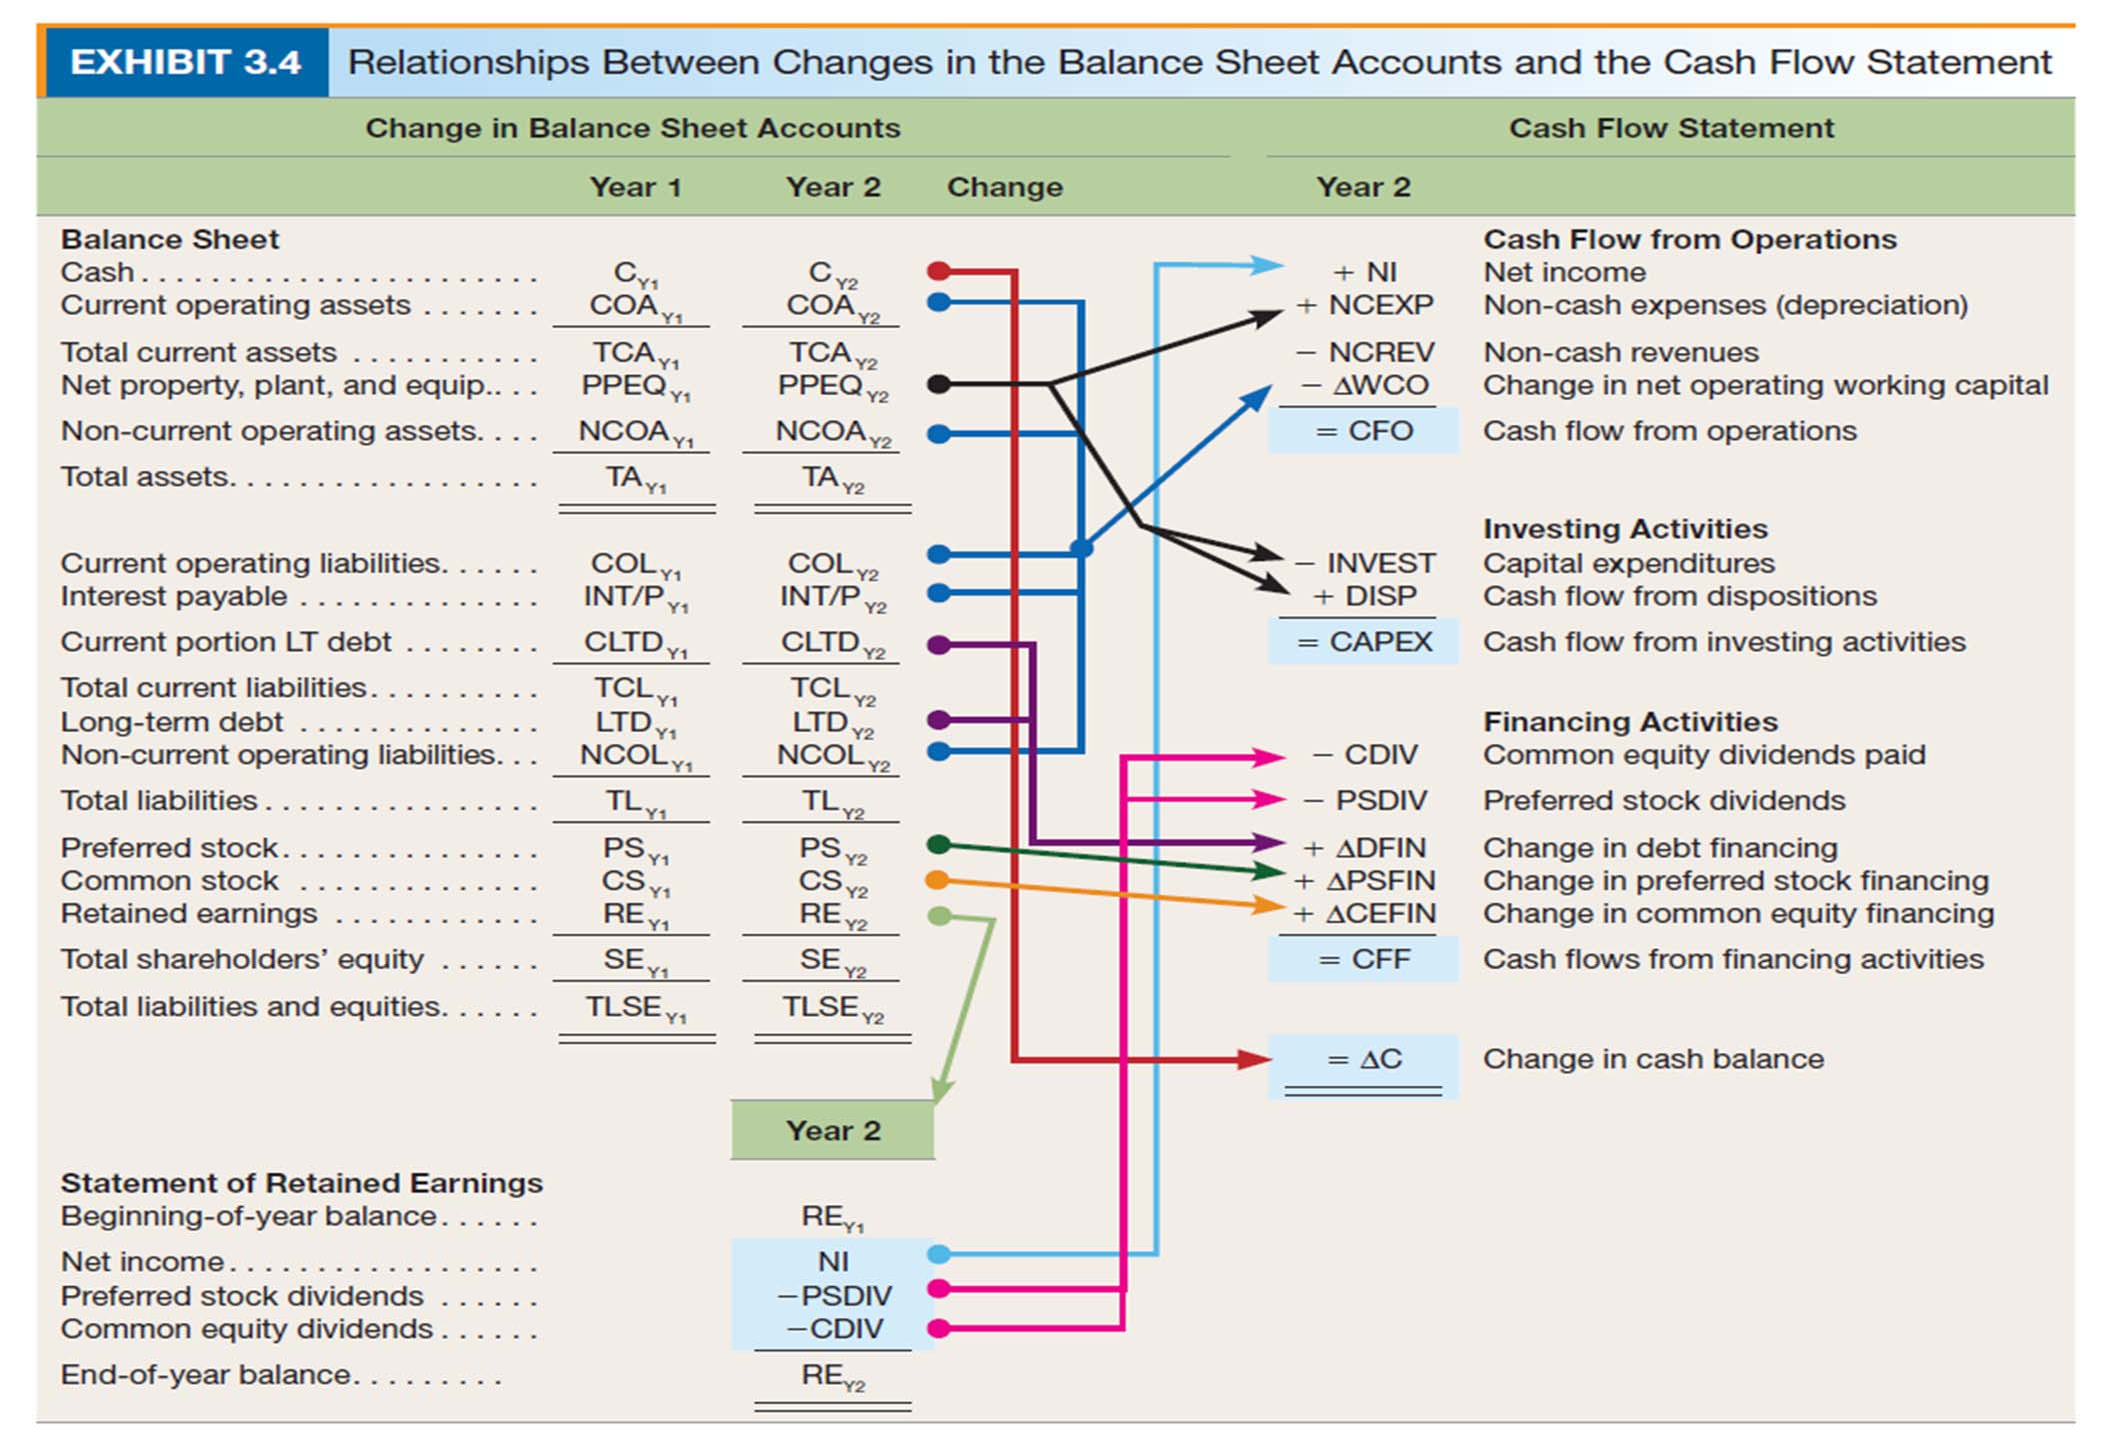
\includegraphics[width=\textwidth]{exhibit34.png}
\caption{Holthausen--Zmijewski, Exhibit 3.4: relationships between changes in the balance-sheet accounts and the cash-flow statement (slide screenshot).}
\end{figure}

Reading the arrows of Exhibit 3.4:
\begin{center}
\small
\begin{tabularx}{\textwidth}{@{}Xl@{}}
\toprule
\textbf{Change in balance-sheet account} & \textbf{Line of the cash-flow statement}\\
\midrule
$\Delta$ Cash ($C$) & $=\Delta C$ (change in cash balance)\\
$\Delta$ Current operating assets (COA), $\Delta$ non-current operating assets (NCOA), $\Delta$ current operating liabilities (COL), $\Delta$ interest payable (INT/P), $\Delta$ non-current operating liabilities (NCOL) & $-\Delta$WCO (in CFO)\\
$\Delta$ Net PP\&E (PPEQ) & $+$NCEXP (CFO); $-$INVEST, $+$DISP (investing)\\
$\Delta$ Current portion of LT debt (CLTD), $\Delta$ long-term debt (LTD) & $+\Delta$DFIN\\
$\Delta$ Preferred stock (PS) & $+\Delta$PSFIN\\
$\Delta$ Common stock (CS) & $+\Delta$CEFIN\\
$\Delta$ Retained earnings: $RE_{Y1}+NI-PSDIV-CDIV=RE_{Y2}$ & $+$NI (CFO); $-$PSDIV, $-$CDIV (financing)\\
\bottomrule
\end{tabularx}
\end{center}

\begin{keybox}[Cash-flow statement]
\begin{align*}
\text{CFO} &= \text{NI} + \text{NCEXP} - \text{NCREV} - \Delta\text{WCO}\\
\text{Cash flow from investing (CAPEX)} &= -\text{INVEST} + \text{DISP}\\
\text{CFF} &= -\text{CDIV} - \text{PSDIV} + \Delta\text{DFIN} + \Delta\text{PSFIN} + \Delta\text{CEFIN}\\
\Delta \text{C} &= \text{CFO} + \text{Investing} + \text{CFF}
\end{align*}
\end{keybox}

\subsubsection*{Mechanics -- Part 2: Exhibit 3.8 (cash-flow statement $\to$ free-cash-flow schedule)}

\begin{figure}[H]
\centering
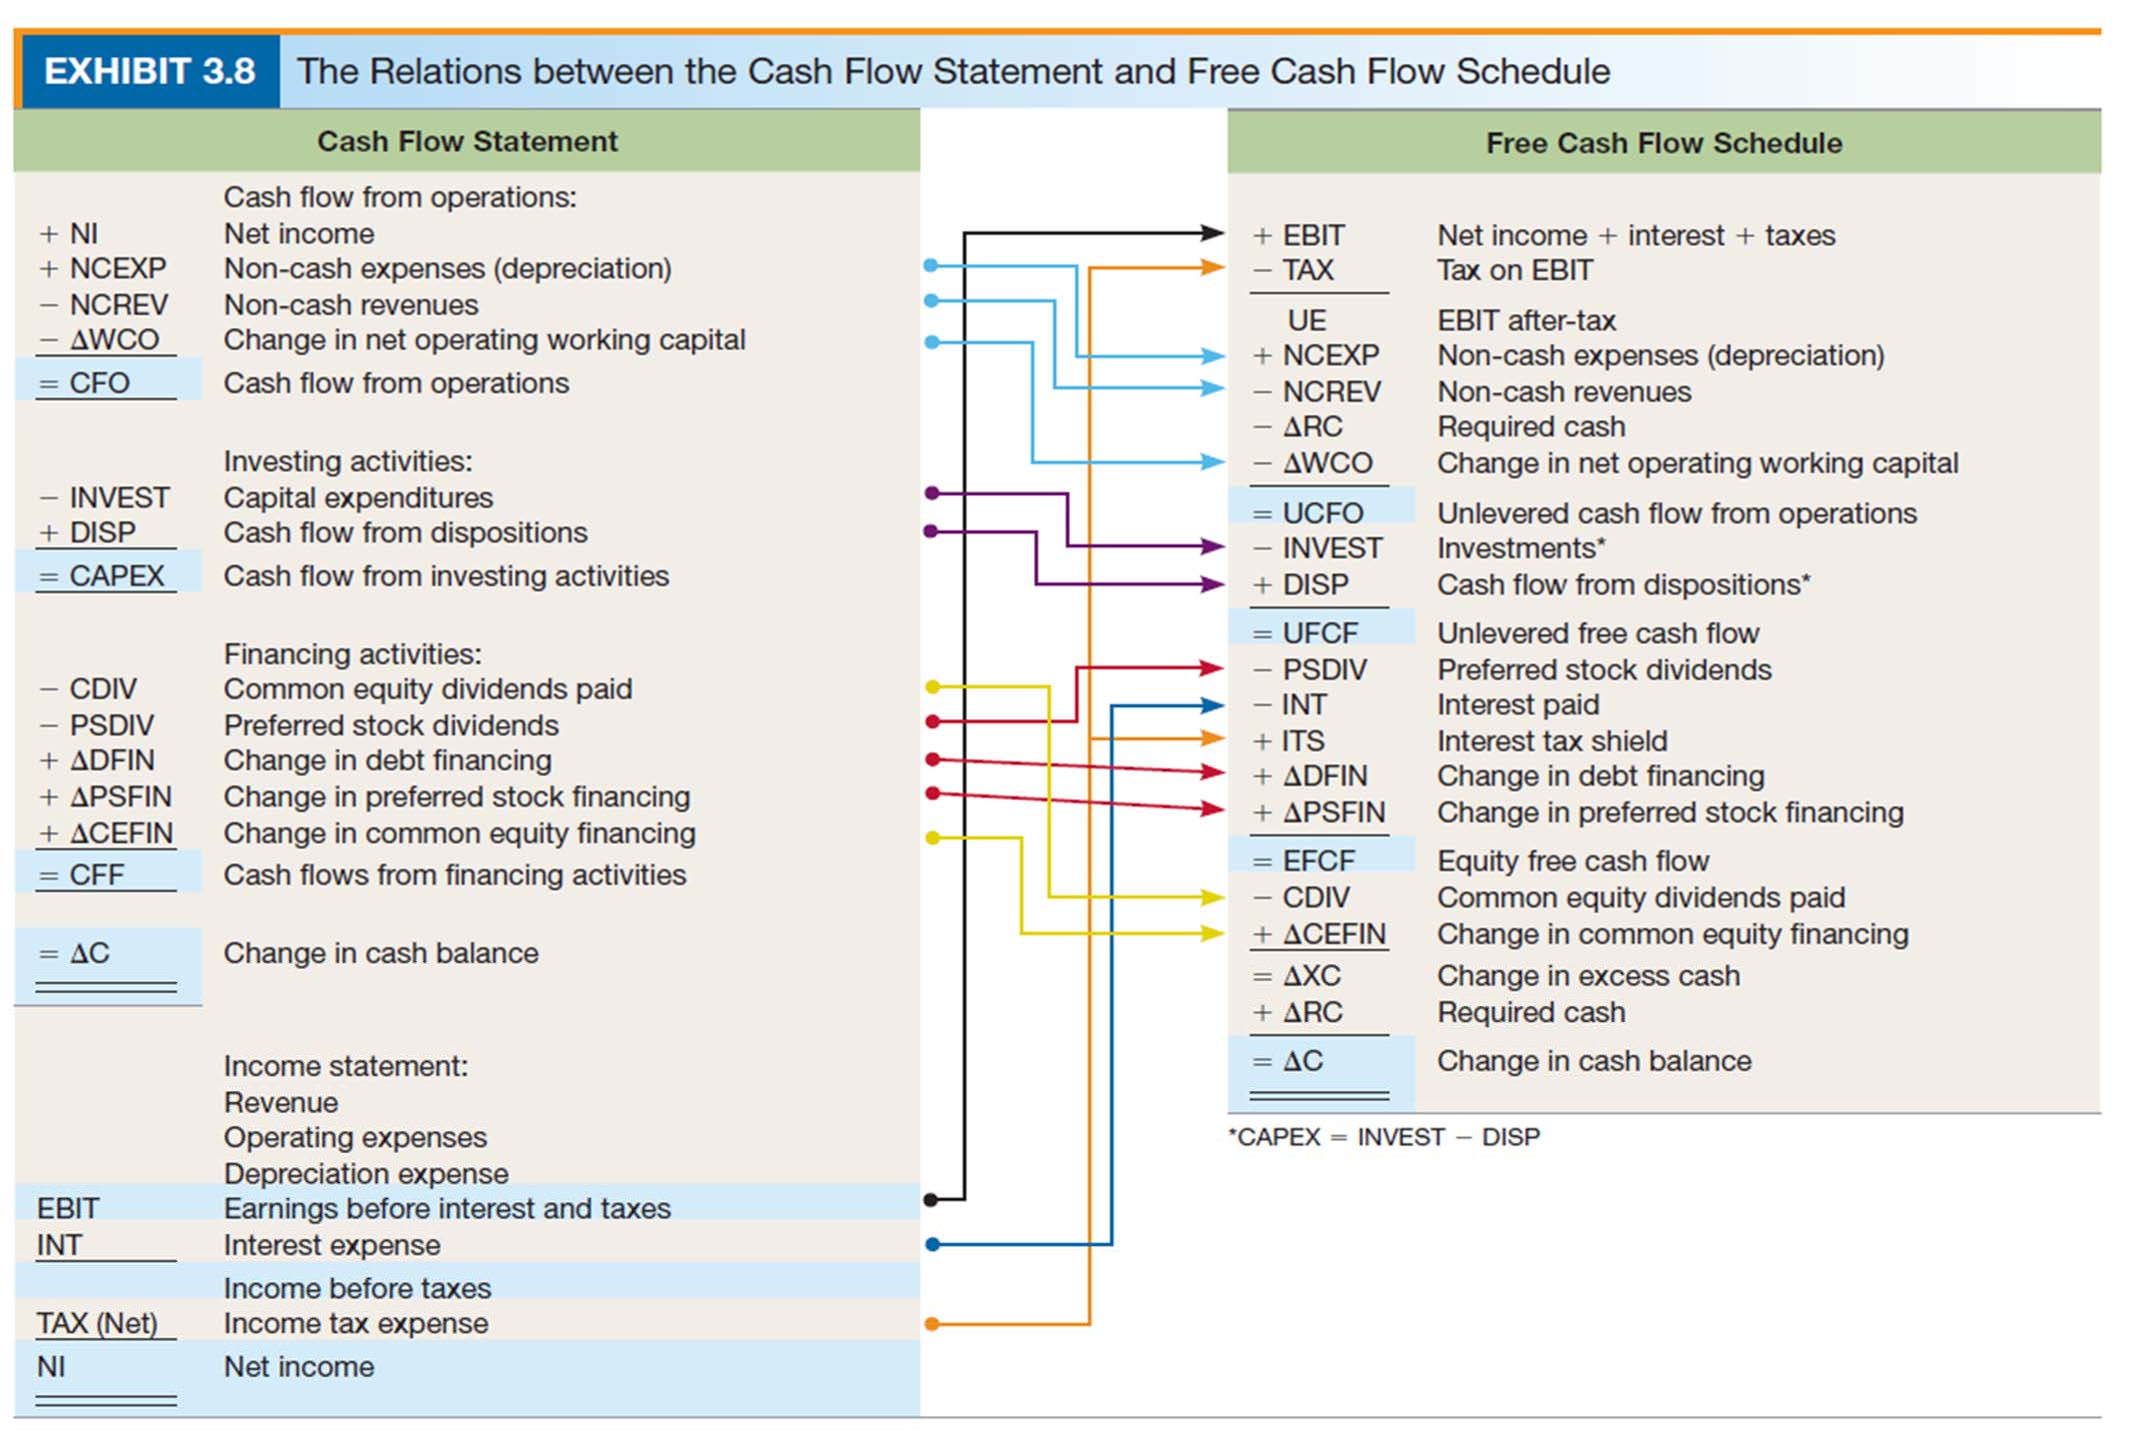
\includegraphics[width=\textwidth]{exhibit38.png}
\caption{Holthausen--Zmijewski, Exhibit 3.8: relations between the cash-flow statement and the free-cash-flow schedule (slide screenshot).}
\end{figure}

\begin{center}
\small
\begin{tabular}{@{}rll@{}}
\toprule
& \textbf{Line} & \textbf{Meaning}\\
\midrule
$+$ & EBIT & Net income + interest + taxes\\
$-$ & TAX & Tax on EBIT\\
\cmidrule{2-3}
& UE & EBIT after tax\\
$+$ & NCEXP & Non-cash expenses (depreciation)\\
$-$ & NCREV & Non-cash revenues\\
$-$ & $\Delta$RC & Required cash\\
$-$ & $\Delta$WCO & Change in net operating working capital\\
\cmidrule{2-3}
$=$ & \textbf{UCFO} & Unlevered cash flow from operations\\
$-$ & INVEST & Investments$^*$\\
$+$ & DISP & Cash flow from dispositions$^*$\\
\cmidrule{2-3}
$=$ & \textbf{UFCF} & \textbf{Unlevered free cash flow ($=$ FCFO)}\\
$-$ & PSDIV & Preferred stock dividends\\
$-$ & INT & Interest paid\\
$+$ & ITS & Interest tax shield\\
$+$ & $\Delta$DFIN & Change in debt financing\\
$+$ & $\Delta$PSFIN & Change in preferred stock financing\\
\cmidrule{2-3}
$=$ & \textbf{EFCF} & \textbf{Equity free cash flow ($=$ FCFE)}\\
$-$ & CDIV & Common equity dividends paid\\
$+$ & $\Delta$CEFIN & Change in common equity financing\\
\cmidrule{2-3}
$=$ & $\Delta$XC & Change in excess cash\\
$+$ & $\Delta$RC & Required cash\\
\cmidrule{2-3}
$=$ & $\Delta$C & Change in cash balance\\
\bottomrule
\multicolumn{3}{@{}l}{\footnotesize $^*$CAPEX $=$ INVEST $-$ DISP}
\end{tabular}
\end{center}

\begin{addbox}[What Exhibit 3.8 teaches]
\begin{enumerate}[leftmargin=*]
  \item The free-cash-flow schedule ends at the \textbf{same $\Delta C$} as the cash-flow statement, so the two reconcile.
  \item \textbf{Required cash} (the cash needed to run the business) is an \textbf{operating} investment, subtracted in UCFO like working capital. \textbf{Excess cash} is what is left after paying shareholders.
  \item \textbf{Tax on EBIT $\neq$ income-tax expense}: TAX on EBIT $=$ tax expense $+$ interest tax shield, with ITS $=t\times$INT. The ITS is given back to equity holders in EFCF.
  \item Dividends are \textbf{not} in FCFE; they are a \textbf{use} of FCFE: FCFE $-$ dividends $+$ new equity $=$ change in excess cash.
\end{enumerate}
\end{addbox}

\subsection{Two Cash-Flow Definitions to Remember}

\begin{keybox}[The two definitions -- memorize]
\begin{align*}
\text{FCFO} &= \text{EBIT}\times(1-\text{tax rate}) + \text{non-cash charges} - \text{CapEx} - \text{increase in non-cash WC}\\[4pt]
\text{FCFE} &= \text{net income} + \text{non-cash charges} - \text{CapEx} - \text{increase in non-cash WC}\\
&\quad + \text{net debt issued}
\end{align*}
\end{keybox}

\subsection{Cash-Flow Definitions in Full}

\begin{center}
\small\begin{tabular}{@{}rl@{\hspace{0.8cm}}rl@{}}
\multicolumn{2}{@{}l}{\textbf{1. FCFE -- equity-side valuation}} & \multicolumn{2}{l}{\textbf{2. FCFO -- asset-side valuation}}\\[3pt]
$+$ & Net income -- adjusted & $+$ & FCFE\\
$+/-$ & Non-cash expenditure (other than D\&A) & $+$ & Interest expense $\times(1-$tax rate$)$\\
& \quad / non-cash revenues & $+$ & (Principal debt repayments\\
$-$ & Net CapEx ($=$ CapEx $-$ D\&A) && \quad $-$ new debt issues)\\
\cmidrule{3-4}
$-$ & Changes in non-cash working capital & $=$ & \textbf{FCFO}\\[6pt]
$-$ & (Principal debt repayments & $+$ & Operating income (EBIT) -- adjusted\\
& \quad $-$ new debt issues) & $+/-$ & Non-cash expenditure (other than D\&A)\\
\cmidrule{1-2}
$=$ & \textbf{FCFE} && \quad / non-cash revenues\\
&& $-$ & Taxes on EBIT\\
&& $-$ & Reinvestment needs (net CapEx and WC)\\
\cmidrule{3-4}
&& $=$ & \textbf{FCFO}
\end{tabular}
\end{center}
\slidefig{[Ignoring preferred dividends. If preferred stock exists, preferred dividends also need to be netted out.]}

\begin{keybox}[FCFE $\leftrightarrow$ FCFO]
\[
\text{FCFE} = \text{FCFO} - \text{Interest}\times(1-t) + (\text{New debt issues} - \text{Principal repayments})
\]
\end{keybox}

\begin{addbox}[Proof that the two routes agree]
$NI=(\text{EBIT}-\text{Int})(1-t)=\text{EBIT}(1-t)-\text{Int}(1-t)$. Substituting into FCFE:
\[
\text{FCFE}=\underbrace{\text{EBIT}(1-t)+\text{D\&A}-\text{CapEx}-\Delta\text{WC}}_{\text{FCFO}}-\text{Int}(1-t)+\text{Net borrowing}.
\]
\end{addbox}

\subsection[Discussion Question]{Discussion Question \layer{PRACTICE}}

\begin{exbox}[Discussion Question -- data]
\begin{center}
\begin{tabular}{@{}lr@{}}
EBIT & \$400\\
Interest expensed and paid & \$100\\
Income tax rate on all income & 40\%\\
Net income & \$180\\
Depreciation & \$200\\
Capital expenditures & \$540\\
Increase in required non-cash working capital & \$80\\
Increase in required cash & \$20\\
Increase in debt financing & \$400\\
Paid-in common dividends & \$90\\
Change in cash balance on balance sheet & \$70\\
Cash flow from operations & \$300\\
\end{tabular}
\end{center}
(i) Prepare the cash-flow statement forecast; (ii) prepare the FCFO forecast; (iii) prepare the FCFE forecast.
\end{exbox}

\begin{exbox}[Solution -- \checkmark\ confirmed by the official class solution (CF-BVal\_02\_Bocconi\_2023\_SOL.xlsx, ``The Example Co'')]
\textbf{Check net income:} EBT $=400-100=300$; taxes $=300\times40\%=120$; NI $=300-120=180$ \checkmark

\medskip
\begin{minipage}[t]{0.47\textwidth}
\textbf{(i) Cash-flow statement}\\[3pt]
\begin{tabular}{@{}lr@{}}
Net income & 180\\
+ Depreciation & 200\\
$-$ Increase in non-cash WC & (80)\\
\midrule
\textbf{= CFO} & \textbf{300} \checkmark\\[3pt]
$-$ Capital expenditures & (540)\\
\midrule
\textbf{= Cash flow from investing} & \textbf{(540)}\\[3pt]
+ Increase in debt & 400\\
$-$ Common dividends & (90)\\
\midrule
\textbf{= CFF} & \textbf{310}\\[3pt]
\textbf{$\Delta$ Cash} $=300-540+310$ & \textbf{70} \checkmark
\end{tabular}
\end{minipage}\hfill
\begin{minipage}[t]{0.47\textwidth}
\textbf{(ii) FCFO}\\[3pt]
\begin{tabular}{@{}lr@{}}
EBIT & 400\\
$-$ Tax on EBIT ($400\times40\%$) & (160)\\
\midrule
= EBIT$(1-t)$ & 240\\
+ Depreciation & 200\\
$-$ Increase in required cash & (20)\\
$-$ Increase in non-cash WC & (80)\\
\midrule
= UCFO & 340\\
$-$ Capital expenditures & (540)\\
\midrule
\textbf{= FCFO} & \textbf{(200)}
\end{tabular}
\end{minipage}

\medskip
\textbf{(iii) FCFE}\\[3pt]
\begin{tabular}{@{}lr@{}}
FCFO & (200)\\
$-$ Interest paid & (100)\\
+ Interest tax shield ($100\times40\%$) & 40\\
+ Net debt issued & 400\\
\midrule
\textbf{= FCFE} & \textbf{140}
\end{tabular}

\medskip
Check from net income: FCFE $=180+200-540-80-20+400=\mathbf{140}$ \checkmark

\textbf{Reconciliation:} FCFE $140-$ dividends $90=$ change in excess cash $50$; $+$ increase in required cash $20=$ \textbf{change in cash $70$} \checkmark\ (matches the balance sheet).

\textbf{Notes.} Tax on EBIT (160) $\neq$ taxes actually paid (120); the difference (40) is the interest tax shield. If required cash were ignored, FCFO would be $-180$. The lecture stresses that ``required cash is not excess cash'', so required cash is an operating need and FCFO $=-200$ (the official solution confirms $-200$).
\end{exbox}

\begin{exbox}[Official solution, third schedule: from CFO to FCFO]
The class solution also derives FCFO starting from the cash-flow-statement CFO, undoing the financing items that CFO contains:
\begin{center}
\begin{tabular}{@{}llr@{}}
\toprule
Cash flow from operations & $+$ CFO & 300\\
$+$ Interest paid in cash & $+$ CINT & 100\\
$-$ Interest tax shield ($40\%\times100$) & $-$ ITS & (40)\\
$-$ Change in required cash & $-\Delta$RC & (20)\\
\midrule
Unlevered cash flow from operations & $=$ UCFO & 340\\
$-$ Capital expenditures & $-$ CAPEX & (540)\\
\midrule
\textbf{Unlevered free cash flow} & $=$ \textbf{FCF} & \textbf{(200)}\\
\bottomrule
\end{tabular}
\end{center}
Logic: CFO starts from net income, so it is \emph{after} interest net of its tax shield ($100\times(1-0.4)=60$). Adding back interest (100) and removing the tax shield (40) gives back exactly those 60, i.e.\ the unlevered figure. Required cash, which CFO ignores, is an operating investment. The official FCF schedule also shows the line \emph{Cash flow before changes in financing} (CFBFIN) $=$ FCF $-$ interest $+$ ITS $-$ preferred dividends $=-200-100+40=-260$, then $+400$ of new debt $=$ EFCF 140.
\end{exbox}

\textbf{What these Discussion Questions test} (slide):
\begin{enumerate}
  \item \textbf{CFO is not FCFO} (300 vs $-200$: CFO is after interest and before CapEx).
  \item \textbf{FCFO excludes (debt) financing} (the 400 of new debt does not enter FCFO).
  \item \textbf{FCFE includes net debt issuance} ($+400$).
  \item \textbf{Dividends are a use of FCFE, not part of FCFO} (the 90 appears only after FCFE).
  \item \textbf{Required cash is not excess cash} (the 20 is an operating investment).
\end{enumerate}

\begin{addbox}
FCFO is negative here because the firm is in an investment phase (CapEx 540 $\gg$ depreciation 200). A negative FCFO is not ``bad'' in itself, since a growing firm reinvests. Here it was financed with new debt, which makes FCFE positive.
\end{addbox}

\subsection{Cash-Flow Definitions: Interpretation}

\begin{itemize}
  \item These concepts apply to \textbf{projections} used in valuation techniques.
  \item \textbf{FCFO}, also known as \textbf{Free Cash Flow to Firm (FCFF)}: the cash flows generated by the operating business. In FCFO the taxes measure the \textbf{theoretical fiscal outflow on the operating result in a scenario of no debt}.
  \item \textbf{FCFE}: the net cash flows available to shareholders. Its value depends not only on interest and income taxes but also on the \textbf{change in the net financial position}. Therefore the projections for the valuation must include a \textbf{target for the firm's financial structure}, because FCFE depends on future financing choices involving debt.
\end{itemize}

% =====================================================================
\subsection{From Reported to Actual Earnings}

\begin{center}
\begin{tikzpicture}[font=\small,
  bx/.style={draw,rounded corners=3pt,align=center,inner sep=4pt,fill=white,drop shadow},
  ln/.style={-{Stealth},thick}]
\node[bx] (h) at (0,3) {Firm's\\history};
\node[bx] (c) at (2.1,3) {Comparable\\Firms};
\node[bx,align=left] (ol) at (4.9,3) {\textbf{\emph{Operating leases}}\\- Convert into debt\\- Adjust operating\\\ \ income};
\node[bx,align=left] (rd) at (8.5,3) {\textbf{\emph{R\&D Expenses}}\\- Convert into asset\\- Adjust operating\\\ \ income};
\node[bx] (n) at (1.05,0.9) {\textbf{Normalize}\\\textbf{Earnings}};
\node[bx,align=left] (cl) at (6.7,0.9) {\textbf{Cleanse} operating items of\\- Financial Expenses\\- Capital Expenses\\- Non-recurring expense};
\node[draw=navy,thick,ellipse,fill=boxblue,font=\normalsize\bfseries] (m) at (4,-0.9) {Measuring Earnings};
\node[bx,draw=teal,align=left] (u) at (7.6,-2.2) {\textbf{Update}\\- Trailing Earnings\\- Unofficial numbers};
\draw[thick] (h.south) |- (1.05,2.1) -| (c.south); \draw[ln] (1.05,2.1) -- (n.north);
\draw[thick] (ol.south) |- (6.7,1.95) -| (rd.south); \draw[ln] (6.7,1.95) -- (cl.north);
\draw[thick] (n.south) |- (4,-0.15) ; \draw[thick] (cl.south) |- (4,-0.15); \draw[ln] (4,-0.15) -- (m.north);
\draw[ln] (u.west) -| (4,-1.35);
\end{tikzpicture}
\end{center}

\subsubsection*{Adjusting accounting earnings}
\begin{enumerate}
  \item \textbf{Make sure no financial expenses are mixed in with operating expenses.}
  \begin{itemize}
    \item \textbf{Financial expense}: any \textbf{tax-deductible commitment that you have to meet no matter what your operating results}. Failure to meet it leads to loss of control of the business.
    \item Example -- \textbf{operating leases}: accounting convention may treat them as operating expenses, but they are really financial expenses and must be reclassified. \textbf{This has no effect on equity earnings but does change the operating earnings.}
  \end{itemize}
  \item \textbf{Make sure no capital expenses (CAPEX) are mixed in with operating expenses (OPEX).}
  \begin{itemize}
    \item \textbf{Capital expense}: any expense that is expected to generate \textbf{benefits over multiple periods}.
    \item Example -- \textbf{R\&D}: since R\&D is a capital expenditure (rather than an operating expense), the operating income has to be adjusted to reflect its treatment.
  \end{itemize}
\end{enumerate}

\subsection{Operating Leases}

\begin{center}
\begin{tikzpicture}
\begin{axis}[ybar,width=11cm,height=5.5cm,bar width=24pt,ymin=0,ymax=60,
  ylabel={\% of operating income},yticklabel={\pgfmathprintnumber{\tick}\%},
  symbolic x coords={Market,Apparel Stores,Furniture Stores,Restaurants},xtick=data,
  xticklabel style={align=center,text width=1.8cm},xticklabels={Market,Apparel\\Stores,Furniture\\Stores,Restaurants},
  title={\small Operating lease expenses as \% of operating income},
  nodes near coords={\pgfmathprintnumber{\pgfplotspointmeta}\%},nodes near coords style={font=\scriptsize},
  ymajorgrids,tick label style={font=\small},enlarge x limits=0.18]
\addplot[fill=navy!45,draw=navy] coordinates {(Market,12.5) (Apparel Stores,43.5) (Furniture Stores,49.5) (Restaurants,26.5)};
\end{axis}
\end{tikzpicture}
\slidefig{Values read from the slide's bar chart (approximate). Leases matter most for retailers and restaurants.}
\end{center}

\begin{itemize}
  \item Operating lease expenses may be treated as operating expenses in computing operating income.
  \item More appropriately, they should be treated as \textbf{financing expenses}, with the following adjustments to earnings and capital:
  \begin{itemize}
    \item \textbf{Debt value of operating leases = PV of operating lease commitments at the pre-tax cost of debt.}
    \item When you convert operating leases into debt, you also create an \textbf{asset of the same value} to counter it.
  \end{itemize}
\end{itemize}

\begin{keybox}[Adjusted operating earnings]
\begin{align*}
\text{Adj.\ operating earnings} &= \text{Operating earnings} + \text{Op.\ lease expense}\\
&\quad - \text{Depreciation on leased asset}\\
\intertext{As an approximation:}
\text{Adj.\ operating earnings} &\approx \text{Operating earnings} + \text{Pre-tax cost of debt}\times\text{PV of op.\ leases}
\end{align*}
\end{keybox}

\begin{addbox}
A lease payment is economically interest + repayment of a loan. Adding back the whole payment and subtracting only the depreciation of the leased asset removes the financing cost (the implicit interest) from operating expenses. The approximation adds back only the imputed interest ($k_d\times$ lease debt), on the assumption that depreciation $\approx$ the principal part of the payment.
\end{addbox}

\begin{exbox}[Worked example: The GAP]
GAP has EBIT of \$1,012m and debt of \$1.97bn; pre-tax cost of debt $6\%$. Operating lease payments this year \$978m. Commitments:
\begin{center}
\begin{tabular}{@{}crcr@{}}
\toprule
\textbf{Year} & \textbf{Commitment (\$m)} & \textbf{$1/1.06^t$} & \textbf{PV at 6\%}\\
\midrule
1 & 899.00 & 0.94340 & 848.11\\
2 & 846.00 & 0.89000 & 752.94\\
3 & 738.00 & 0.83962 & 619.64\\
4 & 598.00 & 0.79209 & 473.67\\
5 & 477.00 & 0.74726 & 356.44\\
6 & 982.50 & 0.70496 & 692.62\\
7 & 982.50 & 0.66506 & 653.42\\
\midrule
6 \& 7 & 982.50 each year & & \textbf{1,346.04}\\
\multicolumn{3}{@{}r}{\textbf{Debt value of leases} (also value of leased asset) $=$} & \textbf{4,396.85}\\
\bottomrule
\end{tabular}
\end{center}
\textcolor{keyred}{\textbf{Slide typo:}} the slide shows \$1,356.04 for years 6--7; the correct value is \textbf{\$1,346.04}, the only figure consistent with the slide's total of \$4,396.85.

\begin{align*}
\text{Adjusted debt outstanding} &= 1{,}970 + 4{,}397 = \mathbf{\$6{,}367m}\\
\text{Adjusted EBIT} &= \text{Reported EBIT} + \text{OL exp.\ this year} - \text{Depreciation}\\
&= 1{,}012 + 978 - \tfrac{4{,}397}{7} = 1{,}012+978-628 = \mathbf{\$1{,}362m}\\[-2pt] &\qquad\text{(7-year useful life of the leased assets, straight line)}\\
\text{Approximate EBIT} &= 1{,}012 + 4{,}397\times6\% = 1{,}012+264 = \mathbf{\$1{,}276m}
\end{align*}
\added Commitments beyond year 5 are often disclosed as a lump sum (here $1{,}965=2\times982.5$) and spread evenly over the remaining years.
\end{exbox}

\begin{exbox}[GAP: conventional accounting vs operating leases treated as debt]
\small
\begin{tabularx}{\linewidth}{@{}>{\bfseries}p{2.1cm}XX@{}}
\toprule
& \textbf{\color{keyred}Conventional accounting} & \textbf{\color{keyred}Operating leases treated as debt}\\
\midrule
Income statement & EBIT before leases $=1{,}990$\newline Op.\ leases $=978$\newline EBIT $=1{,}012\ (=1{,}990-978)$ & EBIT before leases $=1{,}990$\newline $-$ Depreciation leased assets $=628$\newline Adjusted EBIT $=1{,}362\ (=1{,}990-628)$\newline \emph{Interest expense rises to reflect the conversion of operating leases into debt.}\\
\midrule
Balance sheet & Off balance sheet (shown neither as debt nor as an asset). Only the conventional debt of \$1,970m is on the balance sheet. & Asset: OL asset 4,397; Liability: OL debt 4,397\newline Total debt $=4{,}397+1{,}970=\$6{,}367$m\\
\midrule
Cost of capital & $8.20\%\cdot\frac{7{,}350}{9{,}320}+4\%\cdot\frac{1{,}970}{9{,}320}=\mathbf{7.31\%}$ & $8.20\%\cdot\frac{7{,}350}{13{,}717}+4\%\cdot\frac{6{,}367}{13{,}717}=\mathbf{6.25\%}$\\
& \multicolumn{2}{l}{\emph{Cost of equity 8.20\%; after-tax cost of debt 4\%; market value of equity 7,350.}}\\
\midrule
ROIC & $\frac{1{,}012(1-0.35)}{3{,}130+1{,}970}=\frac{657.8}{5{,}100}=\mathbf{12.90\%}$ & $\frac{1{,}362(1-0.35)}{3{,}130+6{,}367}=\frac{885.3}{9{,}497}=\mathbf{9.30\%}$\\
& \multicolumn{2}{l}{\emph{Book value of equity 3,130; tax rate 35\%.}}\\
\bottomrule
\end{tabularx}
\smallskip

\footnotesize $9{,}320=7{,}350+1{,}970$; $13{,}717=7{,}350+6{,}367$. Unrounded, the adjusted ROIC is 9.32\%; the slide shows 9.30\%.
\end{exbox}

\begin{addbox}[Summary of the lease effects]
Capitalizing leases: \textbf{EBIT $\uparrow$, debt $\uparrow$, WACC $\downarrow$} (more weight on cheaper debt), \textbf{invested capital $\uparrow\Rightarrow$ ROIC $\downarrow$}. \textbf{Net income/equity earnings are unaffected} (the slide says so explicitly), and equity value is essentially unchanged: EV is higher, but more debt is subtracted.
\end{addbox}

\subsubsection*{IFRS 16}
\begin{itemize}
  \item In January 2016, \textbf{IFRS 16} was issued, superseding \textbf{IAS 17}.
  \item IFRS 16 applies to reporting periods beginning on or after \textbf{January 1st, 2019}.
  \item Under IFRS 16 \textbf{all leases have to be capitalized} (shown on the balance sheet of the lessee).
\end{itemize}

\begin{center}
\begin{tikzpicture}[font=\small,
  r/.style={draw,minimum width=2.4cm,minimum height=0.9cm,align=center},
  m/.style={draw,minimum width=2.3cm,minimum height=0.9cm,align=center,font=\small\itshape}]
\node[r,minimum height=1.1cm,font=\normalsize] (i) at (0,0) {IFRS 16};
\node[m] (f) at (3.6,2.0) {Finance leases};
\node[m] (o) at (3.6,0) {Operating\\leases};
\node[m] (s) at (3.6,-2.1) {Short-term\\\&/or low-value\\leases};
\node[r] (f2) at (7,2.0) {Capitalized};
\node[r] (o2) at (7,0.55) {\underline{Capitalized}};
\node[r] (o3) at (7,-0.55) {Main novelty};
\node[r,font=\small\itshape] (s2) at (7,-2.1) {Optional\\\underline{recognition}\\\underline{exemption}};
\foreach \a/\b in {i/f,i/o,i/s,f/f2,o/o2,o/o3,s/s2} \draw[gray] (\a.east) -- (\b.west);
\end{tikzpicture}
\slidefig{IFRS 16 exempts from capitalization: (i) short-term leases and (ii) leases of low-value assets.}
\end{center}

\begin{addbox}
Under IFRS 16 the accountants have already made the lease adjustment (right-of-use asset + lease liability on the balance sheet; depreciation + interest in the P\&L instead of rent). For the valuation, lease liabilities then belong to debt in the EV $\to$ equity bridge, and you must be consistent: if lease liabilities are treated as debt, the lease payments must not also be deducted as operating costs in FCFO.
\end{addbox}

\subsection{R\&D Expenses}

\begin{center}
\begin{tikzpicture}
\begin{axis}[ybar,width=9cm,height=5.5cm,bar width=26pt,ymin=0,ymax=60,
  ylabel={\% of operating income},yticklabel={\pgfmathprintnumber{\tick}\%},
  symbolic x coords={Market,Petroleum,Computers},xtick=data,
  title={\small R\&D as \% of operating income},
  nodes near coords={\pgfmathprintnumber{\pgfplotspointmeta}\%},nodes near coords style={font=\scriptsize},
  ymajorgrids,enlarge x limits=0.25]
\addplot[fill=navy!45,draw=navy] coordinates {(Market,10.5) (Petroleum,30.5) (Computers,50.2)};
\end{axis}
\end{tikzpicture}
\slidefig{Values read from the slide's bar chart (approximate).}
\end{center}

\begin{exbox}[Worked example: SAP -- capitalizing R\&D]
EBIT before R\&D $=3{,}045$; R\&D assumed to have a \textbf{5-year life} (straight-line amortization: each year's R\&D is amortized by $1/5=20\%$ per year).
\begin{center}
\small
\begin{tabular}{@{}crccr@{}}
\toprule
\textbf{Year} & \textbf{R\&D expense} & \textbf{Unamort.\ portion} & \textbf{Unamort.\ amount} & \textbf{Amort.\ this year}\\
& & & & \textbf{(= R\&D/5)}\\
\midrule
Current & 1,020.02 & 1.00 & 1,020.02 & --\\
$-1$ & 993.99 & 0.80 & 795.19 & \euro198.80\\
$-2$ & 909.39 & 0.60 & 545.63 & \euro181.88\\
$-3$ & 898.25 & 0.40 & 359.30 & \euro179.65\\
$-4$ & 969.38 & 0.20 & 193.88 & \euro193.88\\
$-5$ & 744.67 & 0.00 & 0.00 & \euro148.93\\
\midrule
\textbf{Total} & & & \textbf{2,914.02} & \textbf{903.14}\\
\bottomrule
\end{tabular}
\end{center}
\begin{itemize}
  \item \textbf{Value of research asset $=$ \euro2,914m} (sum of the unamortized portions).
  \item \textbf{Amortization of the research asset in the current year $=$ \euro903m} (sum of each layer's amortization this year).
  \item \textbf{Increase in operating income $=1{,}020-903=$ \euro117m.}
\end{itemize}
\added Convention: the current year's R\&D is not amortized this year; the year $-5$ layer receives its last amortization this year (unamortized portion $1-j/5$ for the layer of year $-j$).
\end{exbox}

\begin{exbox}[SAP: conventional accounting vs capitalized R\&D ($t=36.54\%$)]
\small
\begin{tabularx}{\linewidth}{@{}>{\bfseries}p{2.1cm}XX@{}}
\toprule
& \textbf{\color{keyred}Conventional accounting} & \textbf{\color{keyred}Capitalized R\&D expenses}\\
\midrule
Income statement & EBIT before R\&D $=3{,}045$\newline $-$ R\&D expenses $=1{,}020$\newline Reported EBIT $=2{,}025$\newline Reported EBIT$(1-t)=2{,}025\times0.6346=1{,}285$ & EBIT before R\&D $=3{,}045$\newline $-$ Amortization R\&D $=903$\newline Adjusted EBIT $=2{,}142$ (increase of 117m)\newline Adjusted EBIT$(1-t)=2{,}142\times0.6346=1{,}359$\newline Ignored tax benefit $=(1{,}020-903)\times0.3654=43$\newline Adjusted EBIT after tax benefit $=1{,}359+43=1{,}402$ (increase of 117m)\newline Net income also increases by 117m\\
\midrule
Balance sheet & Off balance sheet. Book value of equity of 3,768m is \textbf{understated} because one of the biggest assets is off the books. & R\&D asset 2,914 $\leftrightarrow$ book equity $+2{,}914$\newline Adjusted book equity $=3{,}768+2{,}914=6{,}682$\\
\midrule
CapEx & Conventional net CapEx of 2m & Adjusted net CapEx $=2+1{,}020-903=119$\\
\midrule
Cash flows & EBIT$(1-t)=1{,}285$\newline $-$ Net CapEx $=2$\newline \textbf{FCFF $=1{,}283$} & Adjusted EBIT$(1-t)=1{,}402$\newline $-$ Adjusted net CapEx $=119$\newline \textbf{FCFF $=1{,}283$}\\
\midrule
ROIC & $\frac{1{,}285}{3{,}768+530}=\mathbf{29.90\%}$ & $\frac{1{,}402}{6{,}682+530}=\mathbf{19.44\%}$\\
& \multicolumn{2}{l}{\emph{Assumption: liabilities $=530$.}}\\
\bottomrule
\end{tabularx}
\end{exbox}

\begin{keybox}[Key insight]
Capitalizing R\&D changes EBIT, invested capital, ROIC and net CapEx, \textbf{but not the free cash flow} (1,283 in both cases): the same $117$ is added to after-tax EBIT and to reinvestment. ROIC falls because invested capital rises by much more (+2,914).
\end{keybox}

\subsubsection*{The tax-benefit correction}
R\&D expenses are \textbf{tax deductible} $\Rightarrow$ when we capitalize them, a tax benefit goes missing. We therefore add the tax savings on the difference between the entire R\&D expense and the amortization of the research asset to the after-tax adjusted EBIT:
\begin{keybox}[R\&D: corrected adjusted EBIT after tax]
\begin{align*}
\textcolor{addgreen}{\text{Adjusted EBIT after tax}_t} &= (\text{EBIT}_t + \text{R\&D}_t - \text{Amort R\&D}_t)\times(1-\tau_C)\\
\textcolor{addgreen}{\text{Additional tax benefit}_t} &= (\text{R\&D}_t - \text{Amort R\&D}_t)\times\tau_C\\
\textcolor{keyred}{\text{Corrected adjusted EBIT after tax}_t} &= \text{Adjusted EBIT after tax}_t + \text{Additional tax benefit}_t\\
&= (\text{EBIT}_t + \text{R\&D}_t - \text{Amort}_t)(1-\tau_C)\\
&\quad + (\text{R\&D}_t - \text{Amort}_t)\,\tau_C\\
&= \boxed{\text{EBIT}_t\,(1-\tau_C) + \text{R\&D}_t - \text{Amort R\&D}_t}
\end{align*}
\textbf{When adjusting EBIT for R\&D capitalization, we can use the pre-tax R\&D expenses and the pre-tax estimated amortization of the R\&D asset.}
\end{keybox}
SAP check: $1{,}285+1{,}020-903=1{,}402$ \checkmark\ (the slide's formula omits a minus sign in the middle line: it should read R\&D$_t-$D\&A R\&D Asset$_t$).

\subsection{Tax Rate}

\subsubsection*{Effective tax rates of US firms}

\begin{center}
\begin{tikzpicture}
\begin{axis}[ybar,width=10cm,height=5.5cm,bar width=16pt,ymin=0,ymax=35,
  ylabel={Frequency},xlabel={Effective tax rate basket},
  symbolic x coords={5\%,10\%,15\%,20\%,25\%,30\%,35\%,40\%},xtick=data,
  title={\small\itshape Effective Tax Rate for U.S. Companies},
  nodes near coords,nodes near coords style={font=\scriptsize},enlarge x limits=0.08]
\addplot[fill=navy!45,draw=navy] coordinates {(5\%,13) (10\%,29) (15\%,26) (20\%,17) (25\%,7) (30\%,4) (35\%,0) (40\%,0)};
\end{axis}
\end{tikzpicture}
\slidefig{Values read from the slide's histogram (approximate). Most firms' effective rates are far below the statutory/marginal rate.}
\end{center}

\subsubsection*{Impact on valuations: the 2018 US tax reform}

\begin{exbox}[Tax reform and aggregate value effects: US equities]
Macro inputs: US T-bond rate (1/1/18) $=2.41\%$; ERP $=5.08\%$.
\begin{center}
\small
\begin{tabular}{@{}lrr@{}}
\toprule
& \textbf{Pre-tax reform} & \textbf{Post-tax reform}\\
\midrule
Beta & 1.07 & 1.07\\
Pre-tax cost of debt & 3.91\% & 3.91\%\\
Marginal tax rate & 38.00\% & 24.00\%\\
Debt to capital ratio & 23.51\% & 23.51\%\\
Revenues & \$12,254.10 & \$12,254.10\\
Operating income (EBIT) & \$1,438.22 & \$1,438.22\\
Effective tax rate & 25.19\% & 20.00\%\\
After-tax return on capital & 12.76\% & 13.65\%\\
Reinvestment rate & 59.27\% & 65.00\%\\
Length of growth period & 5 & 5\\
\midrule
\multicolumn{3}{@{}l}{\emph{Computed values}}\\
Cost of equity & \textcolor{keyred}{7.85\%} & \textcolor{keyred}{7.85\%}\\
After-tax cost of debt & \textcolor{keyred}{2.42\%} & \textcolor{keyred}{2.97\%}\\
Cost of capital & \textcolor{keyred}{6.57\%} & \textcolor{keyred}{6.70\%}\\
After-tax return on capital & \textcolor{keyred}{12.76\%} & \textcolor{keyred}{13.65\%}\\
Reinvestment rate & \textcolor{keyred}{59.27\%} & \textcolor{keyred}{65.00\%}\\
Expected growth rate & 7.56\% & 8.87\%\\
\midrule
\multicolumn{3}{@{}l}{\emph{Value of firm}}\\
PV of FCFF in high growth & \$2,253.08 & \$2,139.72\\
Terminal value & \$30,926.29 & \$34,590.66\\
\textbf{Value of firm today} & \textbf{\$24,750.46} & \textbf{\$27,151.37}\\
\bottomrule
\end{tabular}
\end{center}
Value with old tax code inputs $=\$24{,}751$bn; with new tax code inputs $=\$27{,}151$bn; \textbf{change in value $=\$2{,}400$bn}; \textbf{percentage change $=2{,}400/24{,}751=9.70\%$}.

\medskip
\textbf{Slide annotations.}
\begin{itemize}[leftmargin=*]
  \item \textbf{Marginal tax rate}: the drop in the federal corporate rate from 35\% to 21\% lowers the overall marginal rate (with state \& local taxes) from 38\% to 24\%.
  \item \textbf{Effective tax rate}: the change in the corporate rate on US income and the shift to a regional tax model for global taxes lower the effective rate from 25.19\% to 20\%.
  \item \textbf{Tax effect on debt}: a lower marginal tax rate \textbf{increases} the after-tax cost of debt and the cost of capital (holding the debt ratio fixed).
  \item \textbf{Higher ROIC/reinvestment}: ROIC rises proportionally with the drop in the effective tax rate; capital-expensing rules lead to marginally more reinvestment. \textbf{Expected growth $=$ ROIC $\times$ reinvestment rate.}
\end{itemize}

\medskip
\textbf{Verification of the computed values} \added
\begin{align*}
k_e &= 2.41\% + 1.07\times5.08\% = 7.85\% \quad\text{(CAPM)}\\
k_d(1-t) &= 3.91\%\times(1-0.38)=2.42\%;\qquad 3.91\%\times(1-0.24)=2.97\%\\
\text{WACC}_{\text{pre}} &= 7.85\%\times0.7649+2.42\%\times0.2351=6.57\%\\
\text{WACC}_{\text{post}} &= 7.85\%\times0.7649+2.97\%\times0.2351=6.70\%\\
\text{ROC}_{\text{post}} &= 12.76\%\times\tfrac{1-0.20}{1-0.2519}=13.65\%\\
g &= 12.76\%\times59.27\%=7.56\%;\qquad 13.65\%\times65\%=8.87\%
\end{align*}
\end{exbox}

\begin{addbox}
Two opposite effects. A lower tax rate raises WACC (smaller debt tax shield $\Rightarrow$ value $\downarrow$), but it raises after-tax operating cash flows and growth (value $\uparrow$). The second effect dominates, so value rises by 9.7\%. Note \textbf{which} rate goes where: the \textbf{marginal} rate enters the after-tax cost of debt (tax shield), while the \textbf{effective} rate enters near-term operating cash flows.
\end{addbox}

\subsubsection*{Which tax rate to use (summary)}

The choice is between the \textbf{effective} and the \textbf{marginal} tax rate.
\begin{keybox}[Rule]
\textbf{When doing projections it is safer to use the marginal tax rate}, since the effective one simply reflects differences between accounting and tax books.
\end{keybox}
\begin{enumerate}
  \item \textbf{Marginal tax rate.} Using it tends to bias the after-tax operating income (NOPAT) in the earlier years, but it is more accurate in later years.
  \item \textbf{Effective tax rate} ($=$ taxes due / taxable income). If you use it, \textbf{adjust it towards the marginal rate over time}, because tax-based revenues/expenses should converge to accruals (and thus cash) in the long run (i.e., in perpetuity).
\end{enumerate}
For \textbf{multinational companies}, be careful. Either:
\begin{itemize}
  \item use a \textbf{weighted average of the marginal tax rates}, with weights based on the income the firm derives from each country; or
  \item use the \textbf{marginal tax rate of the country of incorporation}, assuming implicitly that the income will eventually be repatriated (\textbf{safest approach}); or
  \item keep the income from each country separate and apply a different marginal rate to each income statement.
\end{itemize}

% =====================================================================
\section{Reinvestment Needs}

\subsection{Net Capital Expenditures I}

FCFE and FCFF are computed \textbf{after reinvestments}, which include \textbf{net CapEx} (long term) and \textbf{non-cash working capital} (short term):
\begin{itemize}
  \item \textbf{Net CapEx = CapEx $-$ D\&A};
  \item \textbf{Non-cash working capital}: removes \textbf{excess cash} (beyond day-to-day operating needs).
\end{itemize}
Since we estimate FCFE/FCFF starting from earnings after D\&A (net income and EBIT), we add D\&A back to obtain a cash-flow measure:
\begin{keybox}
\begin{align*}
\textcolor{keyred}{\text{Cash flows from operations}} &= \text{EBIT}\times(1-\tau_C) + \text{Non-cash expenses (e.g., D\&A)}\\
&\quad - \text{Non-cash revenues}
\end{align*}
\end{keybox}
\begin{itemize}
  \item D\&A must be adjusted \textbf{consistently with the adjustments made to earnings} (D\&A of capitalized operating leases, R\&D expenses, \dots).
  \item \textbf{Net CapEx is a function of how fast a firm is growing} or expects to grow: high-growth firms have much higher net CapEx than low-growth ones.
  \item Assumptions about net CapEx can therefore \textbf{never be made independently of assumptions about future growth}.
\end{itemize}

\begin{addbox}
In a no-growth steady state, CapEx $\approx$ D\&A (maintenance only) $\Rightarrow$ net CapEx $\approx0$. Growth requires net CapEx $>0$. This anticipates the relation \emph{expected growth $=$ ROIC $\times$ reinvestment rate} (tax-reform slide and later chapters).
\end{addbox}

\subsection{Net Capital Expenditures II}

When estimating net CapEx, we need to account for:

\textbf{1. The need to smooth lumpy CapEx.} Firms seldom have smooth CapEx, so we normalize it:
\begin{keybox}
\[
\textcolor{keyred}{\text{Estimated net CapEx}} = \frac{1}{n}\sum_{i=1}^{n}\text{CapEx}_{t-i} - \text{D\&A}_t
\]
\end{keybox}
Important caveats: (i) \textbf{do not average D\&A}, since it is already smoothed; (ii) choose carefully the number of historical years used to average CapEx; (iii) check the industry average ratios of (a) \textbf{CapEx/D\&A (preferred)} and/or (b) CapEx/Sales.

\textbf{2. Acquisitions of other firms.} Since these are like CapEx, we need to normalize them:
\begin{keybox}
\begin{align*}
\textcolor{keyred}{\text{Adjusted net CapEx}} &= \text{Net CapEx} + \text{Acquisitions of other firms}\\
&\quad - \text{D\&A of such acquisitions}_t
\end{align*}
\end{keybox}
Important caveats: (i) most firms do not make acquisitions every year, so normalize the measure of acquisitions (e.g., an average over time); (ii) you may ignore acquisitions if you think they were made at fair value (i.e., zero-NPV investments, also accounting for synergies), \textbf{but be careful when estimating growth: growth from acquisitions should then be excluded}.

\begin{exbox}[Illustration (not on slides)]
CapEx in the last 4 years: 80, 200, 60, 100 $\Rightarrow$ average $=440/4=110$. Current D\&A $=70$.\\
Estimated net CapEx $=110-70=\mathbf{40}$ (not $100-70=30$; and D\&A is \emph{not} averaged).
\end{exbox}

\subsection{Net Capital Expenditures III: CapEx Accounted as OpEx}

\textbf{3.} If we decide to re-categorize some OpEx as CapEx, we must estimate the adjusted net CapEx consistently:
\begin{keybox}
\begin{align*}
\text{a) }\ \textcolor{keyred}{\text{Adjusted CapEx}_t} &= \text{CapEx}_t + \text{R\&D expenses}_t\\
\text{b) }\ \textcolor{keyred}{\text{Adjusted D\&A}_t} &= \text{D\&A}_t + \text{R\&D asset amortization}_t\\
\text{c) }\ \textcolor{keyred}{\text{Adjusted net CapEx}_t} &= \text{Adjusted CapEx}_t - \text{Adjusted D\&A}_t\\
&= \text{CapEx}_t + \text{R\&D}_t - \text{D\&A}_t - \text{R\&D amortization}_t\\
&= \text{Net CapEx}_t + \text{R\&D}_t - \text{R\&D amortization}_t
\end{align*}
\end{keybox}
\begin{itemize}
  \item The adjustment made to net CapEx \textbf{mirrors} the adjustment made to EBIT (SAP: $+117$ on both).
  \item We need to make \textbf{consistent adjustments to operating earnings and to net CapEx}.
\end{itemize}

\subsection{Changes in Non-Cash Working Capital}

The second component of reinvestment is the cash for working-capital needs.

\begin{defbox}[Non-cash working capital]
\begin{enumerate}[leftmargin=*]
  \item \textbf{Remove cash and investments in marketable securities in excess of the cash needed for day-to-day operations.} That excess cash should be either (i) \textbf{deducted from the debt value} when estimating the cost of capital, or (ii) \textbf{included as a surplus asset} in the valuation.
  \item \textbf{Remove interest-bearing debt included in current liabilities}, because it has to be considered when computing the debt value for the cost of capital.
\end{enumerate}
\end{defbox}
\begin{itemize}
  \item Changes in non-cash WC from year to year tend to be \textbf{volatile}. A better estimate looks at non-cash WC as a \textbf{\% of revenues} (for the firm and the industry).
  \item Some firms have \textbf{negative non-cash WC}. If this continues it generates positive cash flows for the firm. This is feasible for some time but not forever, so it is better to \textbf{set non-cash WC to zero in perpetuity} when it is negative over the first years of the estimates.
\end{itemize}

\begin{exbox}[Volatility of changes in working capital]
\begin{center}
\begin{tabular}{@{}lrrr@{}}
\toprule
& \textbf{Amazon} & \textbf{Cisco} & \textbf{Motorola}\\
\midrule
Revenues & \$1,640 & \$12,154 & \$30,931\\
Non-cash WC & $-\$419$ & $-\$404$ & \$2,547\\
\% of revenues & $-25.53\%$ & $-3.32\%$ & 8.23\%\\
Change from last year & $-\$309$ & $-\$700$ & $-\$829$\\
Average: last 3 years & $-15.16\%$ & $-3.16\%$ & 8.91\%\\
Average: industry & 8.71\% & $-2.71\%$ & 7.04\%\\
\midrule
\multicolumn{4}{@{}l}{\emph{Assumptions in valuation}}\\
WC as \% of revenue & 3.00\% (?) & $-3.32\%$ & 8.23\%\\
$\Delta$WC as \% of revenue in perpetuity & 25.53\% (?) & 0\% & 0\%\\
\bottomrule
\end{tabular}
\end{center}
Check: $-419/1{,}640=-25.5\%$; $-404/12{,}154=-3.32\%$; $2{,}547/30{,}931=8.23\%$.
\end{exbox}

\begin{addbox}
Negative WC means suppliers finance the firm: it pays suppliers later than its customers pay it (typical of Amazon and supermarkets), so growing revenue \emph{releases} cash. Assuming this forever would inflate the terminal value. Amazon's $-25.5\%$ is far from its industry average ($+8.7\%$); the ``(?)'' marks the analyst's judgment in moving it towards a positive figure rather than extrapolating an unsustainable negative WC. With a stable WC/revenue ratio $w$, the change in WC is $\Delta\text{WC}_t=w\times\Delta\text{Revenue}_t$.
\end{addbox}

% =====================================================================
\section{Conclusion}

\subsection{Common Mistakes in Converting Earnings to Cash Flows (slide)}
\begin{enumerate}
  \item Treating \textbf{EBITDA} as free cash flow.
  \item Including \textbf{interest expense} in FCFO.
  \item Forgetting that \textbf{increases in NWC absorb cash}.
  \item Treating \textbf{all cash as excess cash}.
  \item Discounting \textbf{FCFO with cost of equity} or \textbf{FCFE with WACC}.
  \item Adjusting EBIT for leases or R\&D but forgetting the matching \textbf{balance-sheet / CapEx adjustment}.
  \item Moving from EV to equity value using \textbf{only net debt} when there are other claims.
\end{enumerate}

\subsection{Takeaways}
\begin{itemize}
  \item \textbf{Enterprise value and equity value are different valuation objects}: Enterprise Value (Assets Value) $=$ Equity Value $+$ Net Debt.
  \item \textbf{FCFO values the business; FCFE values the equity.}
  \item \textbf{Cash flows $\neq$ earnings.} This requires adjusting for non-cash expenses and revenues, changes in WC, CapEx, and changes in the company's financing, as when preparing a cash-flow statement.
  \item Financial statements must be reorganized into \textbf{operating, financing, and non-core} components.
  \item The most common errors: mixing cash-flow definitions, discount rates, and value objects.
  \item \textbf{Income-tax disclosures are key} to assess the value of a company:
  \begin{itemize}
    \item the average income-tax rate based on the company's books $\neq$ the income-tax rate actually paid;
    \item \textbf{income-tax expense $\neq$ income taxes paid}, and taxes paid are what is used to measure free cash flows;
    \item the differences stem from \textbf{permanent and temporary factors}; temporary differences reverse.
  \end{itemize}
\end{itemize}

\begin{addbox}
\textbf{Permanent} differences (e.g., non-deductible expenses, tax-exempt income) never reverse and change the effective rate for good. \textbf{Temporary} differences (e.g., accelerated tax depreciation) create deferred taxes that reverse over time. This is why the effective rate should converge towards the marginal rate in perpetuity.
\end{addbox}

% =====================================================================
\section{Formula Summary Sheet}

\begin{center}
\small
\renewcommand{\arraystretch}{1.4}
\begin{longtable}{@{}p{4.6cm}p{10.4cm}@{}}
\toprule
\textbf{Concept} & \textbf{Formula}\\
\midrule
\endhead
EV--equity identity & $\text{EV}=\text{Equity value}+\text{Net debt}$\\
Net financial debt & Financial debt $-$ Cash \& cash equivalents\\
Pension provision (DB plans) & $(\text{PBO}-\text{FV plan assets})\times(1-t)$\\
Other debt-like items & Debt-like provisions $\times(1-t)$\\
Full bridge & Equity $=$ EV $-$ Net debt $-$ Pension$(1-t)$ $-$ Debt-like$(1-t)$ $+$ Non-op.\ assets $-$ Minorities\\
Operating NWC & Inventory $+$ Receivables $-$ Payables\\
Net invested capital & NIC $=$ Net fixed assets $+$ NWC\\
Net financial position & Financial liabilities $-$ Cash\\
Cash from current activities & EBITDA $-\Delta$WC\\
FCFO & $\text{EBIT}(1-t)+\text{non-cash charges}-\text{CapEx}-\Delta\text{non-cash WC}$\\
FCFO (net CapEx form) & $\text{EBIT}(1-t)-(\text{CapEx}-\text{D\&A})-\Delta\text{WC}$\\
FCFE & $\text{NI}+\text{non-cash charges}-\text{CapEx}-\Delta\text{WC}+\text{net debt issued}$\\
FCFE $\leftrightarrow$ FCFO & $\text{FCFE}=\text{FCFO}-\text{Int}(1-t)+(\text{New debt}-\text{Repayments})$\\
Tax on EBIT & $t\times\text{EBIT}=\text{Tax expense}+t\times\text{Interest}$\\
Change in excess cash & FCFE $-$ Dividends $+$ New equity\\
Matching principle & FCFO @ WACC $\to$ EV;\quad FCFE @ $k_e$ $\to$ Equity value\\
Lease debt & $\sum_t \text{Commitment}_t/(1+k_{d,\text{pre-tax}})^t$ \quad (= value of leased asset)\\
Adjusted EBIT (leases) & EBIT $+$ Lease expense $-$ Depreciation of leased asset\\
Approx.\ adjusted EBIT (leases) & EBIT $+\,k_{d,\text{pre-tax}}\times$ PV(leases)\\
Adjusted debt & Debt $+$ PV(leases)\\
R\&D asset ($N$-year life) & $\sum_{j=0}^{N-1}\text{R\&D}_{-j}\,(1-j/N)$\\
R\&D amortization this year & $\sum_{j=1}^{N}\text{R\&D}_{-j}/N$\\
Adjusted EBIT (R\&D) & EBIT $+$ R\&D$_t-$ Amort$_t$\\
Corrected adj.\ EBIT after tax & $\text{EBIT}_t(1-\tau)+\text{R\&D}_t-\text{Amort}_t$\\
Adjusted net CapEx (R\&D) & Net CapEx $+$ R\&D$_t-$ Amort$_t$\\
Smoothed net CapEx & $\frac1n\sum_{i=1}^n\text{CapEx}_{t-i}-\text{D\&A}_t$\\
Net CapEx with acquisitions & Net CapEx $+$ Acquisitions $-$ D\&A of acquisitions\\
Cash flows from operations & $\text{EBIT}(1-\tau)+\text{Non-cash exp.}-\text{Non-cash rev.}$\\
Expected growth & $g=\text{ROIC}\times\text{Reinvestment rate}$\\
ROIC & EBIT$(1-t)$ / (BV equity $+$ BV debt) \ {\footnotesize(GAP, SAP; Chs.\ 4, 8 net cash out: BV equity $+$ BV debt $-$ cash)}\\
WACC & $k_e\frac{E}{D+E}+k_d(1-t)\frac{D}{D+E}$\\
CAPM & $k_e=r_f+\beta\times\text{ERP}$\\
$\Delta$WC (stable ratio $w$) & $w\times\Delta$Revenue\\
\bottomrule
\end{longtable}
\end{center}

% =====================================================================
\needspace{14\baselineskip}
\section{Common Mistakes and Exam Traps}

\begin{trapbox}[Exam traps -- Chapter 1]
\begin{enumerate}[leftmargin=*]
  \item \textbf{EBITDA $\neq$ FCF}: EBITDA ignores taxes, CapEx and $\Delta$WC.
  \item \textbf{CFO $\neq$ FCFO}: CFO (cash-flow statement) starts from net income (after interest) and excludes CapEx; FCFO is unlevered and after CapEx. (DQ: CFO 300 vs FCFO $-200$.)
  \item \textbf{Interest never enters FCFO}, and neither does its tax shield: taxes are computed on EBIT as if the firm were unlevered.
  \item \textbf{Tax on EBIT $\neq$ income-tax expense}: the difference is the interest tax shield (DQ: 160 vs 120).
  \item \textbf{Net borrowing enters FCFE, not FCFO.} A firm can have negative FCFO and positive FCFE if it borrows.
  \item \textbf{Dividends are not subtracted in FCFE}; they are a use of FCFE.
  \item \textbf{Required (operating) cash $\neq$ excess cash}: increases in required cash reduce FCFO; only excess cash is netted against debt or added as a non-operating asset.
  \item \textbf{An increase in WC is a cash outflow} (watch the sign); a decrease is an inflow.
  \item \textbf{Matching principle}: FCFO $\leftrightarrow$ WACC $\leftrightarrow$ EV; FCFE $\leftrightarrow k_e \leftrightarrow$ Equity. Distractors will mix them.
  \item \textbf{EV $-$ net debt is not always equity}: also subtract pensions and other debt-like items (after tax) and minorities, and add non-operating assets (if excluded from FCFO).
  \item Pension and debt-like provisions are taken \textbf{after tax} ($\times(1-t)$); the pension adjustment applies only to \textbf{defined benefit} plans.
  \item Book value of debt is common practice, but the \textbf{market value} is conceptually correct when available.
  \item Operating leases: discount the commitments at the \textbf{pre-tax} cost of debt; lease asset $=$ lease debt; adjusted EBIT adds back the \textbf{whole} lease expense and subtracts the \textbf{depreciation} (not the payment).
  \item Lease capitalization: EBIT $\uparrow$, debt $\uparrow$, WACC $\downarrow$ (GAP: 7.31\% $\to$ 6.25\%), ROIC $\downarrow$ (12.90\% $\to$ 9.30\%), \textbf{no effect on equity earnings}.
  \item R\&D capitalization: EBIT $\uparrow$ by (R\&D $-$ amortization), book equity $\uparrow$ by the research asset, net CapEx $\uparrow$ by the same amount, ROIC $\downarrow$ (29.90\% $\to$ 19.44\%), \textbf{FCFF unchanged} (1,283).
  \item R\&D amortization: the \textbf{current} year's R\&D is not amortized; with a 5-year life the year $-5$ layer is fully amortized this year.
  \item When capitalizing R\&D, don't lose the tax deduction: corrected after-tax EBIT $=$ EBIT$(1-\tau)+$ R\&D $-$ amortization (the adjustment is made pre-tax).
  \item Always make \textbf{matching} adjustments: EBIT adjustment $\leftrightarrow$ CapEx/D\&A/balance-sheet adjustment.
  \item Lumpy CapEx: average \textbf{CapEx only}, never D\&A; prefer the industry \textbf{CapEx/D\&A} ratio.
  \item Acquisitions are CapEx; if they are ignored (fair-value deals), exclude acquisition-driven growth.
  \item Non-cash WC excludes \textbf{excess cash} and \textbf{interest-bearing short-term debt}.
  \item Negative WC forever is not credible $\Rightarrow$ set WC to zero in perpetuity.
  \item \textbf{Use the marginal tax rate} in projections (or let the effective rate converge to the marginal one); for multinationals the safest choice is the marginal rate of the country of incorporation.
  \item A lower tax rate $\Rightarrow$ \textbf{higher} after-tax cost of debt $\Rightarrow$ \textbf{higher} WACC (smaller tax shield), yet value can still rise because of higher after-tax cash flows (2018 reform: $+9.7\%$).
  \item Sum-of-parts: reconstruct each business area's costs up to \textbf{EBIT}.
  \item An FCFE valuation requires a \textbf{target financial structure}, because FCFE depends on future borrowing.
  \item Under \textbf{IFRS 16} (from 1 January 2019) operating leases are capitalized; exemptions only for short-term and low-value leases.
\end{enumerate}
\end{trapbox}

\chapter{Business Forecasting for Valuation}\label{ch:forecast}

\emph{Based on Lecture 03 (file L02, 42 slides): ``Business Forecasting for Valuation''. Session 4 of Part One (workflow step: story $\to$ coherent forecasts). Running case: JJ Jones (value drivers $\to$ forecast statements).}

\section{Where We Are in the Valuation Workflow}

Equity story $\to$ Financial statements $\to$ \textbf{Forecasts} $\to$ Cash flows $\to$ Discount rate $\to$ Terminal value $\to$ Multiples $\to$ Value bridge $\to$ Recommendation.

\begin{keybox}[Today]
\textbf{Equity story + financial statements $\longrightarrow$ coherent forecasts $\longrightarrow$ projected cash flows}
\end{keybox}

\textbf{Today's professional task.} You receive a management business plan. Your job is \textbf{not} to copy it into Excel; it is to \textbf{assess whether it is coherent enough to value}:
\begin{itemize}
  \item identify the business story;
  \item translate the story into value drivers;
  \item build integrated forecast statements;
  \item test whether sales, margins, CapEx, working capital and financing assumptions fit together;
  \item understand how JJ Jones' value drivers generate projected statements.
\end{itemize}

\textbf{Plan for today.}
\begin{center}
\small
\begin{tabularx}{\textwidth}{@{}lXX@{}}
\toprule
\textbf{Layer} & \textbf{What we learn} & \textbf{Why it matters}\\
\midrule
CORE & Equity story $\to$ value drivers $\to$ forecast statements & JJ Jones, project\\
CORE & Projecting IS, BS, and CF statements & Integrated valuation model\\
PRO & Market analysis, strategy, actions, assumptions & Professional business planning\\
TECH & Model architecture, cash sweep, circularity & Avoid spreadsheet/model errors\\
RESEARCH PREVIEW & Forecast coherence & Bridge to special topic\\
PRACTICE & JJ Jones & Turn assumptions into statements\\
\bottomrule
\end{tabularx}
\end{center}

% =====================================================================
\section{From Equity Story to Value Drivers}

\subsection{Overview I: The Phases of Business Planning}

Business planning consists of several interrelated phases:
\begin{center}
\begin{tikzpicture}[
  num/.style={fill=navy,text=white,font=\bfseries,minimum width=0.9cm,minimum height=0.95cm},
  txt/.style={draw=gray!60,fill=gray!6,rounded corners=2pt,text width=10cm,minimum height=0.95cm,align=left,font=\small,inner sep=5pt}]
\foreach \i/\t in {1/{Thorough analysis of company features, market(s), positioning and past performance},
                   2/{Definition of precise competitive strategies},
                   3/{Definition of actions needed to pursue these strategies},
                   4/{Definition of quantitative assumptions underpinning forecast financial statements},
                   5/{Preparation of forecast financial statements}}{
  \node[num] (n\i) at (0,-1.15*\i) {\i};
  \node[txt,anchor=west] at (0.6,-1.15*\i) {\t};
}
\end{tikzpicture}
\end{center}

\subsection{Overview II: Numbers Without Narrative}

There are at least \textbf{three significant dangers} when numbers are used without any narrative in constructing valuations:
\begin{center}
\begin{tikzpicture}[b/.style={fill=navy,text=white,rounded corners=3pt,minimum width=3cm,minimum height=1.1cm,align=center,font=\bfseries}]
\node[b] (a) at (0,0) {Plug-\&-point\\exercise};
\node[b] (b) at (4,0) {Spreadsheet\\Nirvana};
\node[b] (c) at (8,0) {No logical tie\\breaker};
\draw[-{Stealth},line width=3pt,navy!30] (a)--(b); \draw[-{Stealth},line width=3pt,navy!30] (b)--(c);
\end{tikzpicture}
\end{center}
In a good valuation, \textbf{numbers are bound together coherently and story-telling is kept grounded with numbers}:
\begin{itemize}
  \item develop a narrative for the business you are valuing or considering investing in;
  \item test the narrative against history, experience and common sense;
  \item convert key parts of the narrative into value drivers;
  \item connect value drivers to a valuation;
  \item keep the feedback loop open.
\end{itemize}
\begin{keybox}[Key message]
A business plan must be both \textbf{narratively credible} and \textbf{financially coherent}.
\end{keybox}
\begin{addbox}
\textbf{Plug-\&-point}: you plug in numbers and point at the output. \textbf{Spreadsheet nirvana}: the model looks precise just because it is detailed. \textbf{No logical tie breaker}: when two analysts disagree, without a story there is no way to decide which number is more reasonable.
\end{addbox}

\subsection[What Is a Coherent Plan?]{What Is a Coherent Plan? \layer{CORE}}

A plan is coherent when:
\begin{enumerate}
  \item the business story explains the value drivers;
  \item value drivers map into financial-statement items;
  \item sales growth is supported by capacity, CapEx, and working capital;
  \item margin improvement has an operational explanation;
  \item financing assumptions are consistent with cash-flow deficits or surpluses;
  \item long-run assumptions are reachable from the explicit forecast period.
\end{enumerate}
\begin{keybox}[Bottom line]
A plan can be \textbf{plausible line by line and still be incoherent as a system}.
\end{keybox}

\textbf{JJ Jones: today's running case.} We will translate a compact set of value drivers into: income-statement forecasts, PPE forecasts, balance-sheet forecasts, free-cash-flow forecasts (Section~\ref{sec:jjjones}).

\subsection[Market Analysis]{Market Analysis \layer{PRO}}

To prepare accurate and coherent forecasts, it is necessary to analyse the markets the firm operates in. The articulation and complexity of the analysis depends on several variables:
\begin{center}
\begin{tikzpicture}[h/.style={fill=navy,text=white,font=\small\bfseries,minimum width=11cm,minimum height=0.55cm},
  d/.style={fill=navy!15,font=\small,minimum width=11cm,minimum height=0.55cm}]
\foreach \i/\a/\b in {0/{Unrelated businesses}/{The firm operates in unrelated businesses (\emph{holding firms})},
                      1/{Different geographical markets}/{The firm operates in different geographical markets (\emph{multinational firms})},
                      2/{Different distribution channels}/{The business units target different distribution channels$^{(1)}$},
                      3/{Residual}/{Hybrid situations that mix the cases above}}{
  \node[h] at (0,-1.9*\i) {\a};
  \node[d] at (0,-1.9*\i-0.55) {\b};
}
\foreach \i in {0,1,2} \draw[-{Stealth},line width=4pt,navy] (0,-1.9*\i-0.9) -- (0,-1.9*\i-1.55);
\end{tikzpicture}
\slidefig{(1) For instance, a firm could sell its products through both its proprietary website and a network of retail stores.}
\end{center}

\subsection[Competitive Strategy]{Competitive Strategy \layer{PRO}}

The competitive strategies should be prepared both at (1) the \textbf{overall company level} and (2) any \textbf{single business-unit level} (if any).
\begin{center}
\begin{tikzpicture}[hd/.style={fill=navy,text=white,font=\small\itshape,minimum width=3.6cm,minimum height=0.55cm},
  it/.style={fill=navy!15,font=\small,minimum width=3.6cm,minimum height=0.5cm}]
\node[draw,dashed,rounded corners,minimum width=9.6cm,minimum height=0.6cm,font=\bfseries] at (2.4,0.7) {Overall competitive strategy};
\node[hd] at (0,0) {Company level}; \node[hd] at (4.8,0) {Business unit level};
\foreach \i/\a/\b in {1/Operating sectors/Geographical markets,2/Legal structure/Competitive positioning,3/Corporate structure/Distribution channel(s),4/Finance structure/Business model,5/Tax planning/Supply chain integration,6/Intangibles/Physical places to occupy}{
  \node[it] at (0,-0.62*\i) {\a}; \node[it] at (4.8,-0.62*\i) {\b};}
\draw[{Stealth}-{Stealth},line width=6pt,gray!40] (1.95,-1.9) -- (2.85,-1.9);
\end{tikzpicture}
\end{center}

\begin{figure}[H]
\centering
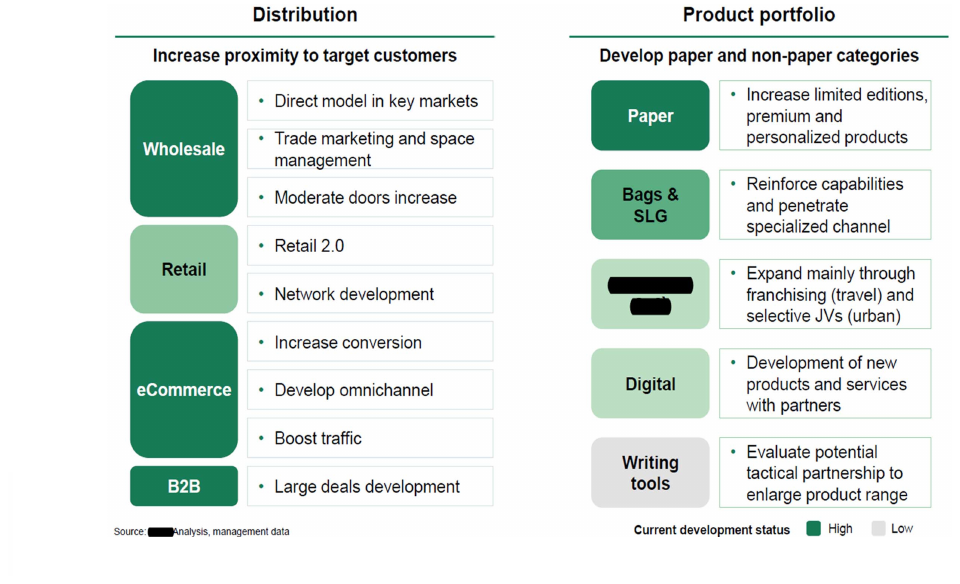
\includegraphics[width=0.85\textwidth]{L02_slide12.png}
\caption{Competitive strategy example (slide screenshot): \textbf{Distribution} -- increase proximity to target customers (Wholesale: direct model in key markets, trade marketing and space management, moderate doors increase; Retail: Retail 2.0, network development; eCommerce: increase conversion, develop omnichannel, boost traffic; B2B: large deals). \textbf{Product portfolio} -- develop paper and non-paper categories (Paper, Bags \& SLG, a redacted category, Digital, Writing tools).}
\end{figure}

\subsection[Action-Taking]{Action-Taking \layer{CORE}}

Once the competitive strategies are defined, the focus is on the \textbf{actions needed to implement them}. Each action should be matched with the following prescriptions:
\begin{center}
\begin{tikzpicture}[a/.style={fill=navy,text=white,minimum width=9cm,minimum height=0.75cm,font=\normalsize,anchor=west}]
\foreach \i/\t in {0/Clear objectives to be pursued,1/Impacts on financial statements,2/Expected realization timing,3/Execution risks and people in charge}{
  \node[a] at (0.6*\i,-0.95*\i) {\hspace{0.8cm}\t};
  \draw[fill=white,draw=navy!40] (0.6*\i,-0.95*\i) circle (0.42);}
\end{tikzpicture}
\end{center}
\slidefig{The credibility of a business plan largely depends on how clearly the mapping of the actions to implement it is set out.}

\begin{figure}[H]
\centering
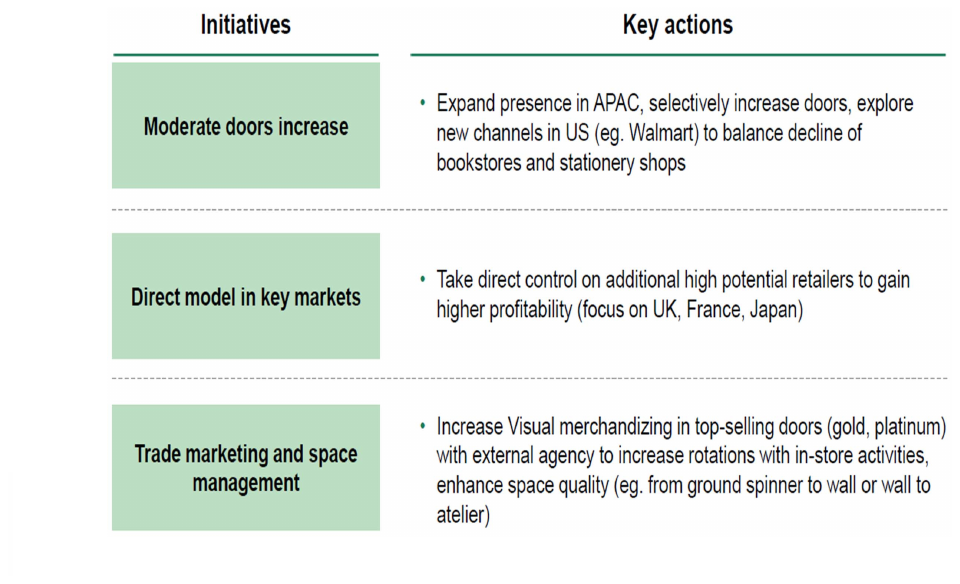
\includegraphics[width=0.72\textwidth]{L02_slide14.png}
\caption{Action-taking example (slide screenshot). \emph{Moderate doors increase}: expand in APAC, selectively increase doors, explore new US channels (e.g., Walmart) to balance the decline of bookstores and stationery shops. \emph{Direct model in key markets}: take direct control of high-potential retailers for higher profitability (UK, France, Japan). \emph{Trade marketing and space management}: visual merchandising in top-selling doors with an external agency, in-store activities, better space quality.}
\end{figure}

\subsection[Quantitative Assumptions]{Quantitative Assumptions \layer{CORE}}

The planning activity ends with a forecast financial statement, based on a series of \textbf{quantitative assumptions}:
\begin{center}
\begin{tabular}{@{}>{\columncolor{navy}\color{white}\bfseries}c p{9cm}@{}}
Macroeconomic & Different for each \emph{geographic area} (GDP, inflation, forex, \dots)\\[3pt]
Business activity & Evolution of \emph{key financials} (sales, costs, working capital, ratios, \dots)\\[3pt]
Corporate structure & Changes at \emph{corporate level} (capital structure, fiscal policy, surplus assets, \dots)
\end{tabular}
\end{center}

\subsection[Revenue Forecast Assumptions]{Revenue Forecast Assumptions \layer{CORE}}

\begin{center}
\begin{tikzpicture}[font=\small,b/.style={draw=navy,minimum width=1.9cm,minimum height=0.55cm,align=center},
  e/.style={-{Stealth[length=1.6mm]},navy}]
\node[b] (rev) at (0,0) {Revenue};
\node[b] (p) at (2.6,1.3) {Price}; \node[b] (v) at (2.6,-1.3) {Volume};
\node[b] (ms) at (5.3,0.2) {Market Size}; \node[b] (sh) at (5.3,-2.6) {Market Share};
\node[b] (g) at (8.0,1.6) {Growth}; \node[b] (t) at (8.0,0.9) {Threats}; \node[b] (o) at (8.0,0.2) {Opportunities};
\node[b] (u) at (8.0,-0.8) {Uniqueness}; \node[b] (aw) at (8.0,-1.5) {Awareness}; \node[b] (lo) at (8.0,-2.2) {Loyalty}; \node[b] (pa) at (8.0,-2.9) {Patents};
\node[b] (ad) at (10.8,0.2) {Advertising}; \node[b] (pr) at (10.8,-0.5) {Promotion}; \node[b] (sf) at (10.8,-1.2) {Sales Force};
\node[b] (dc) at (10.8,-1.95) {Distribution\\[-3pt]Coverage}; \node[b] (av) at (10.8,-2.8) {Availability};
\foreach \x in {p,v} \draw[e] (\x.west) -- (rev.east);
\foreach \x in {ms,sh} \draw[e] (\x.west) -- (v.east);
\foreach \x in {g,t,o} \draw[e] (\x.west) -- (ms.east);
\foreach \x in {u,aw,lo,pa} \draw[e] (\x.west) -- (sh.east);
\foreach \x in {ad,pr,sf,dc,av} \draw[e] (\x.west) -- (u.east);
\end{tikzpicture}
\end{center}
\begin{keybox}[Professional rule]
\textbf{Do not forecast revenue growth as one number unless you can explain the whole logic behind it.}
\[
\text{Revenue} = \text{Price}\times\text{Volume} = \text{Price}\times\text{Market size}\times\text{Market share}
\]
\end{keybox}
\begin{addbox}[Growth decomposition]
$(1+g_{\text{Rev}})=(1+g_{\text{price}})(1+g_{\text{market}})(1+g_{\text{share}})$. Example: price $+2\%$, market $+5\%$, share $+3\%$ $\Rightarrow$ $1.02\times1.05\times1.03-1=10.3\%$.
\end{addbox}

\subsection[Modelling]{Modelling \layer{CORE}}

\begin{center}
\begin{tikzpicture}
\draw[thick,gray!60,fill=navy!5] (-3.2,1.9) -- (3.2,1.9) -- (0.7,-1.3) -- (-0.7,-1.3) -- cycle;
\fill[navy!80] (-1.05,0.85) circle (0.85); \node[text=white,font=\footnotesize\bfseries,align=center] at (-1.05,0.85) {Mkt\\Analysis};
\fill[navy] (1.05,0.85) circle (0.85); \node[text=white,font=\footnotesize\bfseries] at (1.05,0.85) {Strategy};
\fill[navy!55] (0,-0.4) circle (0.75); \node[text=white,font=\footnotesize\bfseries,align=center] at (0,-0.4) {HPs \&\\Actions};
\draw[-{Stealth},line width=6pt,navy!25] (0,-1.35) -- (0,-1.95);
\node[align=center] at (0,-2.4) {\underline{Integrated Forecast Financial Statement}\\{\footnotesize (This is where the equity story becomes numbers)}};
\end{tikzpicture}
\end{center}

% =====================================================================
\section{Building the Integrated Forecast Model}

\subsection[Modelling Basics I--II: The Ten Steps]{Modelling Basics I--II: The Ten Steps \layer{CORE}}

\begin{center}
\begin{tikzpicture}[num/.style={fill=navy,text=white,font=\bfseries,minimum width=0.8cm,minimum height=0.6cm},
  txt/.style={draw=gray!60,fill=gray!6,text width=5.6cm,minimum height=0.6cm,font=\small,inner sep=3pt,anchor=west}]
\foreach \i/\t in {1/Set up the model template,2/Input historical financials,3/Calculate ratios,4/Build assumptions,5/{Project the IS (\underline{leave out interest})}}{
  \node[num] at (0,-0.75*\i) {\i}; \node[txt] at (0.5,-0.75*\i) {\t};}
\foreach \i/\t in {6/{Project the BS (\underline{leave out cash and debt})},7/Project the CF statement,8/Balance the BS,9/{Model interest expense/income},10/{Create summary/output pages}}{
  \node[num] at (7.2,-0.75*\i+3.75) {\i}; \node[txt] at (7.7,-0.75*\i+3.75) {\t};}
\end{tikzpicture}
\end{center}
\begin{addbox}[Why interest, cash and debt come last]
They depend on the financing need, which is only known once operations have been projected. Financing is the last layer and must never ``plug'' operating mistakes.
\end{addbox}

\subsection[Main Aspects and Precautions of Model Set-Up]{Main Aspects and Precautions of Model Set-Up \layer{PRO}}

\textbf{Crucial aspects:}
\begin{enumerate}
  \item One-sheet vs multi-sheet model.
  \item \textbf{Matrix integrity}: a given column refers to a specific year in all sheets.
  \item Key sheets: assumptions/inputs; secondary calculations; debt schedule; income statement; balance sheet; cash-flow statement; summary ratios; output.
\end{enumerate}
\textbf{Precautions:}
\begin{enumerate}
  \item Modelling standards: (a) \textbf{Accurate} -- always proof-read your model (sanity, matrix, and stress check); (b) \textbf{Coherent} -- assumptions about individual items should fit with each other; flexible -- no hard numbers in formulae; user friendly -- break down complex calculations.
  \item Learn keyboard shortcuts (more accurate, more coherent, and more sleep).
  \item Use comments to indicate sources.
  \item Formatting and colour coding: inputs, links to other sheets, and formulae in three different colours (style sheet).
  \item Be able to print your model at any time.
\end{enumerate}

\subsection[Modelling Basics III: Historical Inputs]{Modelling Basics III: Historical Inputs \layer{CORE}}

When collecting historical financial inputs:
\begin{enumerate}
  \item A standard model typically has \textbf{3--5 years} of historical data.
  \item IS and BS line items should reflect the structure of the company's published financials.
  \item Some items must be forecast separately even if not broken down in the financials:
  \begin{itemize}
    \item \textbf{D\&A}: generally included in COGS and SG\&A; find the total in the CF statement;
    \item \textbf{interest expense}: can be expressed net of interest income;
    \item \textbf{interest income}: can be netted from interest expense or included in other income;
    \item \textbf{non-recurring items}: identify them and separate them from the ordinary line items.
  \end{itemize}
  \item Some items may be aggregated for simplicity (other assets/liabilities).
\end{enumerate}

\subsection[Modelling Basics IV: Ratios and Assumptions]{Modelling Basics IV: Ratios and Assumptions \layer{PRO}}

\begin{enumerate}
  \item Identify key ratios to analyse historical performance: IS (growth/margins); BS (days receivable, payable, inventory).
  \item Make assumptions on the evolution of key ratios based on: trends in historical ratios; strategic assessment; market consensus for the company; market consensus for competitors (peer group).
  \item Cross-check the assumptions against: \textbf{historical trends} (any abrupt jumps?); \textbf{internal coherence} (is the evolution of related items coherent?); \textbf{external consistency} (in line with consensus?).
\end{enumerate}

\subsection[Modelling Basics V--VI: Model Architecture]{Modelling Basics V--VI: Model Architecture \layer{TECH}}

\begin{center}
\scriptsize
\begin{tabular}{@{}p{3.7cm}p{4.6cm}p{4.2cm}@{}}
\toprule
\textbf{Income Statement} & \textbf{Retained Earnings} & \textbf{Supporting Schedules}\\
Revenues; Operating expenses; \textbf{EBIT}; Interest expense; EBT; Taxes; \textbf{Net income} &
Beginning balance; + Net income; $-$ Preferred dividends; $-$ Common dividends; = Ending balance &
\emph{Competitive analysis}: general economy, industry, comparables.\newline
\emph{Fixed assets}: capacity needs, fixed-asset requirements, CapEx, depreciation.\\
\midrule
\textbf{Balance Sheet} & \textbf{Free Cash Flows} & \emph{Income taxes}: expense, deferred, NOL carryforward, payable.\\
Operating assets; Fixed assets; \textbf{Total assets}; Operating liabilities; Debt; Total liabilities; Preferred stock; Common stock; Retained earnings; Stockholders' equity; \textbf{Total liabilities + equity} &
EBIT; $-$ Taxes on EBIT; + Non-cash expenses; $-$ $\Delta$Required cash; $-$ $\Delta$Working cap.; $-$ CapEx; = \textbf{Unlevered FCF}; $-$ Interest; + Interest tax shield; $-$ Preferred div.; + $\Delta$Debt; + $\Delta$Preferred; = \textbf{Equity FCF}; $-$ Common div.; = $\Delta$Excess cash; + $\Delta$Required cash; = \textbf{$\Delta$Cash} & \emph{Financing}: debt and interest, preferred stock, common stock.\\
\bottomrule
\end{tabular}
\end{center}

\begin{figure}[H]
\centering
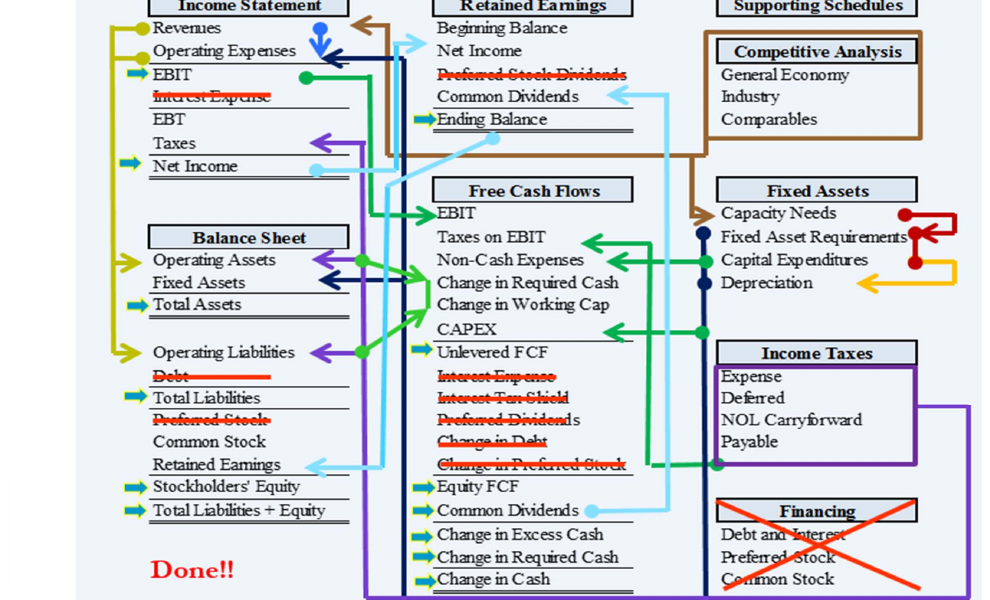
\includegraphics[width=0.85\textwidth]{L02_slide26.png}
\caption{Modelling Basics VI (slide screenshot): how every block of the model links. The financing items (interest expense, debt, preferred stock and dividends, interest tax shield, change in debt and in preferred stock) and the whole Financing schedule are crossed out, and the operating model is ``Done!!''.}
\end{figure}
\begin{addbox}
The message of Modelling Basics VI: the \textbf{operating (unlevered) model} can be completed through the unlevered FCF \textbf{without any financing assumption}. Financing (debt, interest, preferred) is added at the end to balance the BS. This mirrors the split between FCFO (no financing) and FCFE (with financing) in Chapter~\ref{ch:fcf}.
\end{addbox}

\subsection[Projecting the Income Statement]{Projecting the Income Statement \layer{CORE}}

\begin{center}
\begin{tikzpicture}[h/.style={fill=navy,text=white,font=\bfseries,minimum width=7.2cm,minimum height=0.6cm,anchor=north},
  d/.style={fill=navy!15,font=\small,text width=6.9cm,align=center,minimum height=0.6cm,anchor=north,inner sep=3pt}]
\foreach \c/\i/\a/\b in {0/0/{Sales (\emph{forecast growth})}/{Price growth drivers (inflation, strategy); volume growth drivers (tot.\ market \emph{vs} market share)},
                      0/1/{COGS and SG\&A}/{Project COGS and SG\&A as a \% of sales},
                      0/2/{Depreciation}/{Project depreciation as \% of PPE at the \textbf{beginning} of the period},
                      1/0/{Amortization}/{Project amortization based on specific intangible-asset estimation},
                      1/1/{Interest income and expense}/{Leave out until you are done with the rest of the model},
                      1/2/{Taxes}/{Consider effective \emph{vs} marginal tax rate}}{
  \node[h] (h\c\i) at (7.6*\c,-2.95*\i) {\a}; \node[d] (d\c\i) at (h\c\i.south) {\b};}
\foreach \c in {0,1} \foreach \i/\j in {0/1,1/2} \draw[-{Stealth},line width=4pt,navy] ([yshift=-1pt]d\c\i.south) -- ([yshift=1pt]h\c\j.north);
\end{tikzpicture}
\end{center}
\begin{keybox}[Coherence checks]
If revenue grows, do margins, D\&A and capacity assumptions still make sense?\\
If debt, cash, taxes, or interest change, do the projected interest and tax assumptions follow?
\end{keybox}

\textbf{Further issues \layer{PRO}}
\begin{itemize}
  \item \textbf{Net income}: normalize net income for non-recurring items.
  \item \textbf{EPS}: basic \emph{vs} diluted; net income \emph{vs} normalized net income.
  \item \textbf{DPS}: DPS growth rate \emph{vs} payout ratio.
  \item \textbf{Equity}: use net income and dividends to complete the equity base analysis.
\end{itemize}

\subsection[Projecting the Balance Sheet]{Projecting the Balance Sheet \layer{CORE}}

\begin{center}
\small
\begin{tabularx}{\textwidth}{@{}>{\bfseries}p{4.2cm}X@{}}
\toprule
Working capital & Driven by sales and COGS (receivable, inventory and payable days)\\
Fixed assets (PPE schedule in secondary calcs) & CapEx as a fixed component + \% of sales; maintenance \emph{vs} expansion\\
Goodwill & Keep it flat\\
Financial investments \textnormal{(PRO)} & Fair value estimated to stay flat\\
Other operating liabilities \textnormal{(PRO)} & Driven by sales\\
Equity \textnormal{(PRO)} & Take it from the secondary calculation sheet\\
Short and long-term debt \textnormal{(PRO)} & Leave out until you are done with the rest of the model\\
\bottomrule
\end{tabularx}
\end{center}
\begin{keybox}[Coherence checks]
If revenue grows, do receivables, inventories, payables, and PPE grow consistently?\\
Are cash and debt balancing the model, or are they hiding operating-forecast mistakes?
\end{keybox}
\begin{addbox}[Days and ratio formulas used in practice (and in JJ Jones)]
\vspace{-6pt}
\begin{align*}
\text{Receivables} &= \text{Revenue}\times\frac{\text{DSO}}{365} & \text{Inventory} &= \text{COGS}\times\frac{\text{DIO}}{365}\\
\text{Payables} &= \text{COGS}\times\frac{\text{DPO}}{365} & \text{Net PPE} &= \frac{\text{Net PPE}}{\text{Revenue}}\times\text{Revenue}\\
\text{CapEx} &= \Delta\text{Net PPE}+\text{Depreciation}
\end{align*}
\end{addbox}

\subsection[Projecting the Cash-Flow Statement]{Projecting the Cash-Flow Statement \layer{CORE}}

\begin{keybox}[The 100\% rule]
You are \textbf{100\% certain} to be able to obtain the firm's change in cash from the change in all non-cash BS accounts: read that again, you have to be no less than 100\% certain. The CF statement captures the change in every balance-sheet item and yields the resulting change in cash.
\end{keybox}
General rules:
\begin{itemize}
  \item \textbf{Assets up, cash down}; \textbf{liabilities up, cash up};
  \item the change in WC captures changes in operating assets/liabilities;
  \item CapEx and D\&A capture changes in fixed assets;
  \item net income and dividends capture changes in retained earnings.
\end{itemize}

\textbf{Two key cash-flow measures \layer{PRO}}
\begin{center}
\begin{tabular}{@{}rl@{\hspace{1.5cm}}rl@{}}
\multicolumn{2}{@{}l}{\textbf{1. Net cash flow}} & \multicolumn{2}{l}{\textbf{2. Cash available for debt repayment}}\\
$+$ & Operating cash flow & $+$ & Operating cash flow (starting from NI)\\
$+$ & Investing cash flow & $+$ & Investing cash flow\\
$+$ & Financing cash flow & $+$ & Equity issuance\\
\cmidrule{1-2}
$=$ & Net cash flow ($=\Delta$cash) & $-$ & Dividends/stock repurchase\\
\cmidrule{3-4}
&& $=$ & Cash flow available for debt repayment (CFADR)\\
&& $-$ & Cash required (for day-to-day activities)\\
\cmidrule{3-4}
&& $=$ & Cash available for debt repayment (CADR)
\end{tabular}
\end{center}
\begin{keybox}
\begin{gather*}
\text{Beginning cash} + \text{Net cash flow} = \text{Ending cash}\\
\text{Beginning cash} + \text{CFADR} - \text{Cash required} = \text{CADR}
\end{gather*}
\end{keybox}

\subsection[Final Procedures]{Final Procedures \layer{TECH}}

\textbf{I. Balancing the BS.}
\begin{itemize}
  \item Complete the debt schedule.
  \item Use a simple \textbf{cash sweep}: all cash available for debt repayment pays down debt, starting from short-term and moving to long-term debt.
  \begin{itemize}
    \item If CADR is \textbf{positive}, it goes to repay debt.
    \item If CADR is \textbf{negative}, short-term debt is issued to cover the shortage of cash and the minimum level of operating cash required to run operations smoothly.
  \end{itemize}
  \item Link the resulting short-term and long-term debt balances to the BS (in turn reflected in the CF statement), and link the resulting cash balance in the CF statement to the BS.
\end{itemize}

\textbf{II. Circularity.} When interest expense is computed on \textbf{average} debt and interest income on \textbf{average} cash, the model becomes circular:
\begin{center}
\begin{tikzpicture}[c/.style={fill=navy,text=white,rounded corners=3pt,minimum width=2.2cm,minimum height=0.9cm,align=center,font=\small}]
\node[c] (i) at (0,1.5) {Interest\\expenses/income};
\node[c] (n) at (2.6,0) {Net\\income};
\node[c] (c) at (0,-1.5) {Cash flow};
\node[c] (d) at (-2.6,0) {Debt/cash\\ending balance};
\draw[-{Stealth},gray,thick,bend left=25] (i) to (n); \draw[-{Stealth},gray,thick,bend left=25] (n) to (c);
\draw[-{Stealth},gray,thick,bend left=25] (c) to (d); \draw[-{Stealth},gray,thick,bend left=25] (d) to (i);
\end{tikzpicture}
\end{center}
A (less accurate) alternative that does not require iteration is to use the \textbf{opening balance} of debt and cash.

\textbf{III. Summary and output pages} (PRO). Build ratios on projected performance: growth; activity/asset turnover; solvency/credit; profitability; returns. If needed, prepare output sheets that are easy to paste into presentations (a life saver when assumptions change at the last minute, e.g., before a board meeting) and clear when printed from Excel.

% =====================================================================
\section{JJ Jones Case: From Value Drivers to Forecast Statements}\label{sec:jjjones}

\begin{exbox}[JJ Jones: value drivers]
\small
\begin{minipage}[t]{0.48\linewidth}
\textbf{\color{keyred}Income statement}
\begin{itemize}[leftmargin=*]
  \item Revenue growth -- simple 10\% growth
  \item Cost of goods sold -- 60\% of revenues
  \item Operating expenses -- 10\% of revenues
  \item Depreciation -- 10 years
  \item Income tax rate -- 40\% on all income
\end{itemize}
\textbf{\color{keyred}Assets}
\begin{itemize}[leftmargin=*]
  \item Excess assets (cash and other) -- \$0
  \item Required cash balance -- 5\% of revenues
  \item Accounts receivable -- 50 days$^*$
  \item Inventory -- 80 days$^*$
  \item Other current assets -- 6\% of revenues
  \item Net PPE to revenues -- 1.2 ratio$^*$
  \item Other assets -- \$0
\end{itemize}
\end{minipage}\hfill
\begin{minipage}[t]{0.48\linewidth}
\textbf{\color{keyred}Liabilities and preferred stock}
\begin{itemize}[leftmargin=*]
  \item Accounts payable -- 40 days$^*$
  \item Accrued expenses -- 20\% of revenues
  \item Non-current liabilities -- 10\% of revenues
  \item Other income -- \$0 (excess assets related)
  \item Interest rate -- 8\% (beginning balance)
  \item Preferred dividend rate -- 10\% (beginning balance)
  \item Debt -- retire current portion of long-term debt; increase long-term debt if the company has insufficient cash flow (same interest rate)
  \item Preferred stock -- no change
\end{itemize}
\end{minipage}

\smallskip
\footnotesize $^*$ based on ending balance (not average balance)
\end{exbox}

\textbf{Discussion Questions.} Given the value drivers, prepare JJ Jones' (i) income-statement forecasts; (ii) PPE forecasts; (iii) balance-sheet forecasts; (iv) free-cash-flow forecasts.

\textbf{What JJ Jones tests} (slide):
\begin{enumerate}
  \item Can you translate assumptions into forecast statements?
  \item Can you keep the three statements linked?
  \item Can you distinguish required cash from excess cash?
  \item Can you forecast working capital from days ratios?
  \item Can you forecast PPE from the PPE/revenue ratio?
  \item Can you let debt/cash balance the model instead of plugging operations?
  \item Can you compute FCFO and FCFE from the resulting statements?
\end{enumerate}

\begin{addbox}[How each driver becomes a line item]
\begin{itemize}[leftmargin=*]
  \item Revenue$_t$ = 1.10 $\times$ Revenue$_{t-1}$; COGS = 60\%; Opex = 10\%; taxes = 40\% of EBT.
  \item Depreciation = Gross PPE$_{\text{begin}}$ / 10 (10-year straight line).
  \item Net PPE$_t$ = 1.2 $\times$ Revenue$_t$ $\Rightarrow$ CapEx$_t$ = Net PPE$_t$ $-$ Net PPE$_{t-1}$ + Depreciation$_t$.
  \item AR = Rev $\times$ 50/365; Inventory = COGS $\times$ 80/365; AP = COGS $\times$ 40/365 (ending balances).
  \item Interest = 8\% $\times$ beginning debt; preferred dividends = 10\% $\times$ beginning preferred (beginning balances avoid circularity).
  \item Debt is the \textbf{balancing item}: repay the current portion of LTD; if cash flow is insufficient, issue new LTD. Since excess assets $= 0$, any surplus would be paid out (no excess cash accumulates).
\end{itemize}
\end{addbox}

\begin{exbox}[Illustrative one-year forecast (base-year figures assumed by us; the class handout has the real ones)]
\small
\textbf{Assumed base year (Y0):} revenue 1,000; cash 50 (= 5\%); AR $1{,}000\times50/365=136.99$; inventory $600\times80/365=131.51$; other CA 60; gross PPE 2,000, accumulated depreciation 800, net PPE 1,200 (= 1.2 $\times$ revenue); AP $600\times40/365=65.75$; accrued 200; current LTD 50; LTD 500; non-current liabilities 100; preferred 100; common equity (balancing) 562.74.

\medskip
\begin{minipage}[t]{0.47\linewidth}
\textbf{(i) Income statement, Y1}\\[2pt]
\begin{tabular}{@{}lr@{}}
Revenue ($1{,}000\times1.1$) & 1,100.00\\
$-$ COGS (60\%) & (660.00)\\
$-$ Operating expenses (10\%) & (110.00)\\
$-$ Depreciation ($2{,}000/10$) & (200.00)\\
\midrule
EBIT & 130.00\\
$-$ Interest ($8\%\times550$) & (44.00)\\
\midrule
EBT & 86.00\\
$-$ Taxes (40\%) & (34.40)\\
\midrule
\textbf{Net income} & \textbf{51.60}\\
$-$ Preferred dividends ($10\%\times100$) & (10.00)
\end{tabular}

\medskip
\textbf{(ii) PPE, Y1}\\[2pt]
\begin{tabular}{@{}lr@{}}
Net PPE ($1.2\times1{,}100$) & 1,320.00\\
CapEx ($1{,}320-1{,}200+200$) & 320.00\\
Gross PPE ($2{,}000+320$) & 2,320.00\\
Accum.\ depreciation ($800+200$) & 1,000.00
\end{tabular}
\end{minipage}\hfill
\begin{minipage}[t]{0.51\linewidth}
\textbf{(iii) Balance sheet, Y1}\\[2pt]
\begin{tabular}{@{}lr@{}}
Required cash ($5\%\times1{,}100$) & 55.00\\
AR ($1{,}100\times50/365$) & 150.68\\
Inventory ($660\times80/365$) & 144.66\\
Other CA ($6\%$) & 66.00\\
Net PPE & 1,320.00\\
\midrule
\textbf{Total assets} & \textbf{1,736.34}\\[3pt]
AP ($660\times40/365$) & 72.33\\
Accrued ($20\%$) & 220.00\\
LTD ($500+129.67$) & 629.67\\
Non-current liab.\ ($10\%$) & 110.00\\
Preferred stock & 100.00\\
Common equity \footnotesize($562.74+51.6-10$) & 604.34\\
\midrule
\textbf{Total L + E} & \textbf{1,736.34} \checkmark
\end{tabular}
\end{minipage}

\medskip
\textbf{Debt as balancing item.} $\Delta$ net operating WC $=\Delta$AR $13.70+\Delta$Inv $13.15+\Delta$OCA $6.00-\Delta$AP $6.58-\Delta$Accrued $20-\Delta$NCL $10=-3.73$ (a release of cash).\\
CFO $=51.60+200+3.73=255.33$; then $-$CapEx 320 $-$ preferred dividends 10 $-$ repayment of current LTD 50 $-\Delta$required cash 5 $=-129.67$ $\Rightarrow$ \textbf{new LTD issued $=129.67$}; common dividends $=0$; excess cash $=0$. (For simplicity, no new current portion of LTD is scheduled in Y1.)

\medskip
\textbf{(iv) Free cash flows, Y1}\\[2pt]
\begin{tabular}{@{}lr@{\hspace{0.8cm}}lr@{}}
EBIT$(1-t)=130\times0.6$ & 78.00 & FCFO & (43.27)\\
+ Depreciation & 200.00 & $-$ Interest $\times(1-t)=44\times0.6$ & (26.40)\\
$-\Delta$Required cash & (5.00) & $-$ Preferred dividends & (10.00)\\
$-\Delta$Net operating WC & 3.73 & + Net debt ($129.67-50$) & 79.67\\
$-$ CapEx & (320.00) & & \\
\cmidrule{1-2}\cmidrule{3-4}
\textbf{FCFO} & \textbf{(43.27)} & \textbf{FCFE} & \textbf{0.00}
\end{tabular}

\medskip
Check: FCFE $0.00$ = common dividends $0$ + $\Delta$excess cash $0$ \checkmark. FCFE is exactly zero because debt is the balancing item and no excess cash or dividends are allowed: all of the operating deficit is financed with debt.
\end{exbox}

% =====================================================================
\section{Conclusion}

\subsection{Common Mistakes in Business Forecasting (slide)}
\begin{enumerate}
  \item Forecasting a \textbf{hockey stick} without explaining the operational mechanism.
  \item Forecasting the \textbf{most likely case} instead of \textbf{expected cash flows}.
  \item Growing sales while leaving \textbf{CapEx or working capital flat}.
  \item Improving margins without explaining \textbf{pricing power, cost efficiency, or mix}.
  \item Ignoring \textbf{cyclicality} and normalizing the wrong year.
  \item Letting \textbf{cash or debt become the hidden plug}.
  \item Treating the business plan as a \textbf{spreadsheet exercise} rather than a story-to-numbers exercise.
\end{enumerate}

\begin{addbox}[On ``most likely'' vs ``expected'']
DCF needs the \textbf{mean} (probability-weighted) cash flows. With skewed outcomes (e.g., a 70\% chance of 100 and a 30\% chance of 0), the most likely case is 100 but the expected value is $0.7\times100+0.3\times0=70$. Discounting the most likely case overstates value.
\end{addbox}

\subsection{Takeaways}
\begin{enumerate}
  \item A business plan starts with a story, but it is only useful for valuation when the story becomes \textbf{value drivers}.
  \item Forecasts must be \textbf{integrated}: IS, BS, CF statement, debt schedule, and outputs must reconcile.
  \item Revenue growth should be decomposed into \textbf{price, volume, market size, and market share} whenever possible.
  \item CapEx and working-capital assumptions must be coherent with sales growth and capacity needs.
  \item A good model does not hide problems in cash, debt, or plug variables.
  \item JJ Jones is our first full exercise in translating value drivers into forecast statements and cash flows.
\end{enumerate}

% =====================================================================
\section{Formula Summary Sheet}

\begin{center}
\small
\renewcommand{\arraystretch}{1.4}
\begin{tabular}{@{}p{5cm}p{10cm}@{}}
\toprule
\textbf{Concept} & \textbf{Formula}\\
\midrule
Revenue decomposition & Revenue $=$ Price $\times$ Volume $=$ Price $\times$ Market size $\times$ Market share\\
Growth decomposition & $(1+g)=(1+g_{\text{price}})(1+g_{\text{market}})(1+g_{\text{share}})$\\
Receivables & Revenue $\times$ DSO/365\\
Inventory & COGS $\times$ DIO/365\\
Payables & COGS $\times$ DPO/365\\
Net PPE & (Net PPE/Revenue) $\times$ Revenue\\
CapEx & $\Delta$Net PPE $+$ Depreciation\\
Depreciation & Gross PPE$_{\text{begin}}$/useful life, or \% of beginning PPE\\
Interest (no circularity) & Rate $\times$ beginning debt\\
Cash identity & Beginning cash $+$ Net cash flow $=$ Ending cash\\
CFADR & CFO $+$ CFI $+$ Equity issuance $-$ Dividends/repurchases\\
CADR & Beginning cash $+$ CFADR $-$ Cash required\\
CF rules & Assets $\uparrow\Rightarrow$ cash $\downarrow$; Liabilities $\uparrow\Rightarrow$ cash $\uparrow$\\
FCFO & EBIT$(1-t)+$ Dep $-\Delta$WC $-\Delta$Required cash $-$ CapEx\\
FCFE & FCFO $-$ Int$(1-t)$ $-$ Pref.\ div.\ $+$ Net debt issued\\
Expected cash flow & $\sum_s p_s\,CF_s$ (not the most likely case)\\
\bottomrule
\end{tabular}
\end{center}

% =====================================================================
\needspace{14\baselineskip}
\section{Common Mistakes and Exam Traps}

\begin{trapbox}[Exam traps -- Chapter 2]
\begin{enumerate}[leftmargin=*]
  \item The order of the 10 modelling steps: the IS is projected \textbf{without interest}, the BS \textbf{without cash and debt}; interest is modelled after balancing (step 9).
  \item Cash and debt must \textbf{balance} the model, not hide operating errors (no hidden plug).
  \item Depreciation is projected on \textbf{beginning-of-period} PPE; interest on \textbf{beginning} debt avoids circularity. Average balances make the model circular (it needs iteration).
  \item Days ratios: receivables on \textbf{revenue}; inventory and payables on \textbf{COGS}; JJ Jones uses \textbf{ending} balances.
  \item Do not forecast revenue growth as a single number: decompose it into price $\times$ volume (market size $\times$ market share).
  \item Sales growth requires matching CapEx and working-capital growth (capacity); flat CapEx with growing sales overstates FCF.
  \item Forecast \textbf{expected} cash flows, not the most likely case.
  \item Cash sweep: positive CADR repays debt, starting from short-term and then long-term; negative CADR $\Rightarrow$ issue short-term debt to cover the shortfall and the minimum operating cash.
  \item Goodwill and financial investments are kept \textbf{flat}; other operating liabilities are driven by sales.
  \item Assets up $\Rightarrow$ cash down; liabilities up $\Rightarrow$ cash up.
  \item A plan can be plausible line by line and incoherent as a system.
  \item Each action must have objectives, financial-statement impact, timing, execution risks and people in charge.
  \item Required cash (5\% of revenue in JJ Jones) $\neq$ excess cash (0 in JJ Jones).
  \item The unlevered model (up to unlevered FCF) needs \textbf{no financing assumption}; FCFE does.
  \item Three dangers of numbers without narrative: plug-\&-point exercise, spreadsheet nirvana, no logical tie breaker.
  \item Historical data: 3--5 years; separate non-recurring items; D\&A total is found in the CF statement.
  \item Cross-check assumptions against historical trends, internal coherence and external consistency (consensus).
\end{enumerate}
\end{trapbox}

\chapter[Special Topic 01: Coherent Plans]{Special Topic 01:\\Coherent Plans}\label{ch:coherent}

\emph{Based on Special Topic 01 (file L03, 16 slides): ``Coherent Plans''. Session 5 of Part One (research-based judgment). Built on S.\ Rossi's paper with P.\ Giustinelli, \emph{The Coherence Side of Rationality: Theory and Evidence from Firm Plans} (forthcoming, \emph{Review of Financial Studies}).}

\section{Where We Are in the Valuation Workflow}

Equity story $\to$ Financial statements $\to$ \textbf{Forecasts} $\to$ \textbf{Cash flows} $\to$ Discount rate $\to$ Terminal value $\to$ Multiples $\to$ Value bridge $\to$ Recommendation.
\begin{keybox}[Today]
\textbf{Forecasts $\longrightarrow$ Cash flows $\longrightarrow$ Value}
\end{keybox}

\section{Why May Good-Looking Forecasts Still Produce Bad Valuations?}

\begin{itemize}
  \item Each assumption may look \textbf{reasonable in isolation}.
  \item The problem is whether the assumptions \textbf{fit together}.
  \item Valuation errors often come from \textbf{inconsistency across revenue, margins, CapEx, working capital, debt, and terminal assumptions}.
\end{itemize}
\begin{keybox}[Bottom line]
The unit of analysis is not a single forecast. It is the \textbf{forecast system}.
\end{keybox}

\section{Coherence Is Not the Same as Accuracy}

\begin{center}
\small
\begin{tabularx}{\textwidth}{@{}lXX@{}}
\toprule
 & \textbf{Accurate ex post} & \textbf{Inaccurate ex post}\\
\midrule
\textbf{Coherent ex ante} & Good process, good outcome & Good process / bad luck / bad outcome\\
\textbf{Incoherent ex ante} & Bad process, lucky outcome & Bad process / bad outcome / \textbf{predictable error}\\
\bottomrule
\end{tabularx}
\end{center}
\begin{keybox}[Main message]
\textbf{Accuracy is judged after realizations; coherence is assessed before realizations.}
\end{keybox}
\begin{addbox}
Coherence is the property you can control and check today, before any outcome is known: do the assumptions fit together as one business? Accuracy depends on outcomes and luck. A coherent plan can turn out wrong (bad luck), and an incoherent plan can turn out right (good luck). But the errors of incoherent plans are \emph{predictable}, i.e., systematic rather than random, which is why they matter for valuation.
\end{addbox}

% =====================================================================
\section{Rules of Thumb in Business Planning}

\subsection{How CFOs and Analysts Often Forecast}

\begin{center}
\begin{tikzpicture}
\node[anchor=north west,text width=12.3cm,font=\small] at (0,0) {
\begin{enumerate}[leftmargin=*]
  \item \textbf{Plain growth} -- compute for each item the average of the 2--3 most recent annual growth rates.
  \item \textbf{Percentage of sales} -- assign to each item the same growth rate as that forecast for sales.
  \item \textbf{Economies of scale} -- estimate an OLS regression of each item's growth on contemporaneous sales growth: the estimated \textbf{intercept is the fixed component}; the estimated \textbf{slope times the forecast sales growth is the variable component}.
  \item \textbf{Industry-based} -- same as 3, but using only data on firms in the same industry.
  \item \textbf{Disaggregated / multivariate} -- estimate a ``kitchen sink'' specification with all available variables.
\end{enumerate}};
\draw[-{Stealth},thick] (13.2,-0.2) -- (13.2,-5.2);
\node[font=\scriptsize,anchor=south] at (13.2,-0.2) {Least coherent};
\node[font=\scriptsize,anchor=north] at (13.2,-5.2) {Most coherent};
\end{tikzpicture}
\end{center}

\begin{addbox}[The economies-of-scale rule in formulas]
For each item $X$ (e.g., COGS), estimate on historical data
\[
g_{X,t} = \alpha + \beta\, g_{\text{Sales},t} + \varepsilon_t
\qquad\Longrightarrow\qquad
\hat g_{X,t+1} = \underbrace{\hat\alpha}_{\text{fixed component}} + \underbrace{\hat\beta\,\hat g_{\text{Sales},t+1}}_{\text{variable component}}
\]
Percentage of sales is the special case $\alpha=0,\ \beta=1$: every item grows exactly like sales. If $\beta<1$ (e.g., costs with a fixed part), margins expand as sales grow (operating leverage).\\
Example: $\hat\alpha=1\%$, $\hat\beta=0.6$, forecast sales growth $10\%$ $\Rightarrow$ cost growth $=1\%+0.6\times10\%=7\%<10\%$, so the margin improves.
\end{addbox}

\subsection{The Misleading Simplicity of ``Everything Grows with Sales''}

\begin{center}
\small
\begin{tabular}{@{}lcl@{}}
\toprule
\textbf{Percentage-of-sales model} & & \textbf{Coherence questions}\\
\midrule
Sales growth forecast/target & $+10\%$ & Does demand, market share, or capacity support this?\\
COGS / SG\&A growth forecast & $+10\%$ & Are there fixed costs or scale economies?\\
Net working capital growth forecast & $+10\%$ & Does working-capital intensity remain constant?\\
Capital expenditures growth forecast & $+10\%$ & Is there maintenance CapEx?\\
\bottomrule
\end{tabular}
\end{center}
\begin{keybox}[Key point]
Percentage-of-sales is \textbf{not wrong by definition}; it is wrong when it \textbf{ignores the economics of the business}.
\end{keybox}

% =====================================================================
\section{The Paper's Findings}

\subsection{Incoherence Is Not Just an Academic Concern}

\begin{enumerate}
  \item \textbf{CFO forecasts often align with rules of thumb.}
  \item \textbf{Some rules are more incoherent than others}:
  \begin{itemize}
    \item \textbf{Plain growth and percentage-of-sales are the most incoherent}; \textbf{multivariate is the most coherent};
    \item \textbf{nearly half} of CFO forecasts align with the plain-growth and percentage-of-sales rules of thumb (RoTs).
  \end{itemize}
  \item \textbf{Incoherence is associated with}: predictable forecast errors; lower performance; underinvestment.
\end{enumerate}

\begin{addbox}[Reading the paper with the six questions of the Introduction]
\begin{itemize}[leftmargin=*]
  \item \textbf{Research question}: are firms' plans internally coherent, and does incoherence matter?
  \item \textbf{Wisdom challenged}: rationality is usually judged on accuracy (are forecasts right on average?); the paper adds a \emph{coherence} dimension (do the forecasts fit together?).
  \item \textbf{Method}: compare CFO forecasts with the forecasts implied by the five rules of thumb.
  \item \textbf{Results}: the three findings above.
  \item \textbf{Professional implication}: test the plan as a system before valuing it.
  \item \textbf{Limitations}: the detailed data and identification are in the paper (on Blackboard), not on the slides.
\end{itemize}
\end{addbox}

\subsection{How Incoherent Plans Distort Valuation}

\begin{center}
\begin{tikzpicture}[b/.style={fill=navy,text=white,rounded corners=2pt,font=\small,align=center,minimum height=0.8cm,inner sep=3pt},ar/.style={-{Stealth},thick,navy}]
\node[b] (a) at (0,0) {Incoherent\\plan};
\node[b] (b) at (2.5,0) {Wrong\\reinvestment};
\node[b] (c) at (5.0,0) {Wrong\\FCFO};
\node[b] (d) at (7.5,0) {Wrong terminal\\value};
\node[b] (e) at (10.6,0) {Wrong EV and\\Equity Value};
\draw[ar] (a)--(b); \draw[ar] (b)--(c); \draw[ar] (c)--(d); \draw[ar] (d)--(e);
\end{tikzpicture}
\end{center}
Examples:
\begin{center}
\small
\begin{tabular}{@{}l@{$\;\longrightarrow\;$}l@{}}
Sales growth without CapEx & FCFO \textbf{overstated}\\
Working capital flat despite growth & cash needs \textbf{understated}\\
Debt/cash used as plug & financing policy \textbf{hides} operating inconsistency\\
Terminal growth not reachable from explicit period & terminal value becomes \textbf{fantasy}\\
Margin expansion without mechanism & terminal margin \textbf{overstated}\\
\end{tabular}
\end{center}

\begin{exbox}[Illustration: sales growth without CapEx (not on slides)]
Year-1 forecast: EBIT $=100$, $t=40\%$, D\&A $=50$, $\Delta$WC $=10$. Revenue grows 10\%.
\begin{itemize}[leftmargin=*]
  \item \textbf{Incoherent plan}: CapEx $=50$ (= D\&A, maintenance only). FCFO $=100\times0.6+50-50-10=\mathbf{50}$.
  \item \textbf{Coherent plan}: growth needs capacity, say net CapEx $=30$ (CapEx $=80$). FCFO $=60+50-80-10=\mathbf{20}$.
\end{itemize}
The incoherent plan overstates FCFO by 150\%, and the error compounds through the terminal value.
\end{exbox}

% =====================================================================
\section{Examples}

\subsection{JJ Jones: Which Assumptions Must Fit Together?}

\begin{center}
\small
\begin{tabular}{@{}p{7cm}p{7cm}@{}}
\textbf{\color{keyred}Income statement} & \textbf{\color{keyred}Liabilities and preferred stock}\\
$\bullet$ Revenue growth -- simple 10\% growth & $\bullet$ Accounts payable -- 40 days$^*$\\
$\bullet$ Cost of goods sold -- 60\% of revenues & $\bullet$ Accrued expenses -- 20\% of revenues\\
$\bullet$ Operating expenses -- 10\% of revenues & $\bullet$ Debt -- retire current portion of LTD, increase LTD if insufficient cash flow (same interest rate)\\[4pt]
\textbf{\color{keyred}Assets} & \\
$\bullet$ Excess assets (cash and other) -- \$0 & \\
$\bullet$ Required cash balance -- 5\% of revenues & \\
$\bullet$ Accounts receivable -- 50 days$^*$ & \\
$\bullet$ Inventory -- 80 days$^*$ & \\
$\bullet$ Net PPE to revenues -- 1.2 ratio$^*$ & \\
\end{tabular}
\end{center}
\begin{itemize}
  \item What else must be true for these assumptions to describe \textbf{one coherent business}?
  \item JJ Jones is not just a modelling exercise; \textbf{it is a coherence exercise}.
\end{itemize}

\begin{addbox}[What else must be true for JJ Jones]
\begin{itemize}[leftmargin=*]
  \item \textbf{Constant margins} (COGS 60\%, opex 10\%) with 10\% growth means no economies of scale: all costs are variable. Is this consistent with the business (rent, staff, overheads)?
  \item \textbf{Net PPE/revenue fixed at 1.2} means every \$1 of extra revenue needs \$1.2 of new net PPE: at 10\% growth, net CapEx $=1.2\times\Delta$Revenue. Capacity is coherent with growth.
  \item \textbf{Days ratios fixed} means WC grows with sales: the WC intensity of the business model does not change.
  \item \textbf{Debt as balancing item} means the financing policy must be consistent with the deficits generated (in the official solution FCFO is $-798$ and FCFE $-2{,}342$ in Year 3, financed by running off 2,400 of excess assets, see Chapter~\ref{ch:forecast}): can the firm keep raising debt at 8\%?
  \item \textbf{10\% growth forever} is not reachable in a terminal value: long-run growth must converge to a sustainable rate.
\end{itemize}
\end{addbox}

\subsection{The Coherence Checklist}

\begin{center}
\small
\renewcommand{\arraystretch}{1.3}\begin{tabularx}{\textwidth}{@{}>{\bfseries\color{navy}\raggedright\arraybackslash}p{5.6cm}X@{}}
\toprule
1. Story-to-driver coherence & Does the equity story explain the forecast drivers?\\
2. Revenue-to-capacity coherence & Does growth require CapEx, capacity, hiring, inventory, or marketing?\\
3. Margin coherence & Do margin changes follow from price, mix, scale, efficiency, or input costs?\\
4. Working-capital coherence & Do receivables, inventory, and payables reflect the business model?\\
5. Financing coherence & Are debt, cash, dividends, and repurchases consistent with FCFE?\\
6. Terminal coherence & Is the terminal firm reachable from the explicit forecast?\\
\bottomrule
\end{tabularx}
\end{center}

\subsection{Plausible Is Not Necessarily Coherent}

\begin{itemize}
  \item Excel can make a model balance even when assumptions are economically inconsistent.
  \item AI can generate plausible narratives and reasonable-looking assumptions.
\end{itemize}
$\Longrightarrow$ \textbf{Neither Excel nor AI guarantees coherence.} The analyst's job is to \textbf{test the system}.
\begin{keybox}[Bottom line]
\textbf{A model that balances is not necessarily a business plan that makes sense.}
\end{keybox}

\subsection[Discussion Question]{Discussion Question \layer{PRACTICE}}

\begin{exbox}[Discussion Question]
Consider the following system of forecasts:
\begin{itemize}
  \item Sales growth 12\% per year
  \item EBITDA margin rises from 15\% to 22\%
  \item CapEx falls below depreciation
  \item NWC remains constant
  \item Debt is repaid quickly
  \item Terminal growth is 4\%
\end{itemize}
(i) Under what business story could this plan be coherent? (ii) Which assumptions are red flags absent that story?
\end{exbox}

\begin{exbox}[Suggested solution (our own, not provided on the slides; built on the coherence checklist)]
\textbf{(i) A story that could make it coherent.} A firm that has \textbf{just completed a large investment cycle} and has \textbf{spare capacity}, so it can grow 12\% without new capacity (CapEx $<$ depreciation is temporarily possible). Growth fills the existing plants, so \textbf{fixed costs are spread over more volume} (operating leverage), explaining the margin expansion from 15\% to 22\%. Alternatively, an \textbf{asset-light / scalable} model (software, platforms) whose growth needs little physical capital. NWC constant is plausible if the firm improves its cash cycle (shorter DSO/DIO, longer DPO) or sells with up-front payment. Strong cash generation then allows fast debt repayment.

\textbf{(ii) Red flags absent that story} (checklist item in brackets):
\begin{enumerate}[leftmargin=*]
  \item \textbf{CapEx below depreciation with 12\% growth} [revenue-to-capacity]: the asset base shrinks while volume grows. That works only while spare capacity lasts; in steady state net CapEx must be positive ($g=\text{ROIC}\times\text{reinvestment rate}$). FCFO is overstated.
  \item \textbf{NWC constant while sales grow 12\%} [working capital]: with unchanged days ratios WC should grow $\approx$12\% per year; cash needs are understated.
  \item \textbf{Margin 15\% $\to$ 22\%} [margin]: requires a mechanism (pricing power, mix, scale, efficiency, input costs); without one, the terminal margin is overstated.
  \item \textbf{Fast debt repayment} [financing]: possible only because FCF is inflated by the previous points. Financing looks healthy because the operating forecast is incoherent.
  \item \textbf{Terminal growth 4\%} [terminal]: high for a perpetuity (around or above long-run nominal GDP growth), and inconsistent with zero or negative net reinvestment. Growth forever needs reinvestment; a terminal value built on these flows ``becomes fantasy''.
\end{enumerate}
\end{exbox}

% =====================================================================
\section{Takeaways}

\begin{enumerate}
  \item Coherence is a property of the \textbf{forecast system (plan)}, not of one forecast variable.
  \item A plan can be plausible line by line and incoherent overall.
  \item Rules of thumb are useful only when they \textbf{respect business economics}.
  \item Incoherent plans distort \textbf{FCFO, terminal value, leverage, and valuation}.
  \item Good analysts test whether story, assumptions, financial statements, and valuation all fit together.
\end{enumerate}
\begin{keybox}[Closing line]
In valuation, discipline is not only getting the formula right. It is \textbf{making the assumptions fit together}.
\end{keybox}

% =====================================================================
\section{Formula Summary Sheet}

\begin{center}
\small
\renewcommand{\arraystretch}{1.4}
\begin{tabular}{@{}p{5.2cm}p{9.8cm}@{}}
\toprule
\textbf{Concept} & \textbf{Formula}\\
\midrule
Plain growth & $\hat g_{X,t+1}=$ average of the last 2--3 annual growth rates of $X$\\
Percentage of sales & $\hat g_{X,t+1}=\hat g_{\text{Sales},t+1}$ (i.e., $X/\text{Sales}$ constant)\\
Economies of scale & $g_{X,t}=\alpha+\beta g_{\text{Sales},t}+\varepsilon_t$; $\hat g_X=\hat\alpha$ (fixed) $+\hat\beta\hat g_{\text{Sales}}$ (variable)\\
Industry-based & Same regression, estimated on same-industry firms only\\
Multivariate & ``Kitchen sink'' regression with all available variables\\
Growth needs reinvestment & $g=\text{ROIC}\times\text{Reinvestment rate}$ (Chapter~\ref{ch:fcf})\\
Coherence vs accuracy & Coherence: ex ante; accuracy: ex post\\
\bottomrule
\end{tabular}
\end{center}

% =====================================================================
\needspace{14\baselineskip}
\section{Common Mistakes and Exam Traps}

\begin{trapbox}[Exam traps -- Chapter 3]
\begin{enumerate}[leftmargin=*]
  \item \textbf{Coherence $\neq$ accuracy}: coherence is assessed \emph{before} realizations, accuracy is judged \emph{after}. A coherent plan can be inaccurate (bad luck); an incoherent plan can be accurate (luck).
  \item Incoherent plans produce \textbf{predictable} (systematic) forecast errors.
  \item Ranking of rules of thumb: \textbf{plain growth} (least coherent) $\to$ percentage of sales $\to$ economies of scale $\to$ industry-based $\to$ \textbf{multivariate} (most coherent).
  \item Paper's findings: CFO forecasts often follow rules of thumb; \textbf{nearly half} follow plain growth or percentage of sales; incoherence is associated with \textbf{predictable forecast errors, lower performance, underinvestment}.
  \item Economies-of-scale rule: \textbf{intercept = fixed component}; \textbf{slope $\times$ forecast sales growth = variable component}.
  \item Percentage of sales is \textbf{not wrong by definition}, only when it ignores the business economics (fixed costs, maintenance CapEx, changing WC intensity).
  \item The unit of analysis is the \textbf{forecast system}, not a single forecast.
  \item Sales growth without CapEx $\Rightarrow$ FCFO \textbf{overstated}; flat WC despite growth $\Rightarrow$ cash needs \textbf{understated}; debt/cash as plug $\Rightarrow$ hides operating inconsistency; unreachable terminal growth $\Rightarrow$ terminal value becomes fantasy; margin expansion without mechanism $\Rightarrow$ terminal margin overstated.
  \item A model that \textbf{balances} is not necessarily coherent; neither Excel nor AI guarantees coherence.
  \item Six coherence checks: story-to-driver, revenue-to-capacity, margin, working capital, financing (consistent with FCFE), terminal (reachable from the explicit forecast).
\end{enumerate}
\end{trapbox}

\chapter[From Cash Flows to Enterprise Value: WACC and APV]{From Cash Flows to Enterprise Value:\\WACC and APV}\label{ch:wacc}

\emph{Based on Lecture 04 (file L04, 31 slides): ``From Cash Flows to Enterprise Value -- WACC, APV, and the role of financing policy''. Sessions 6--7 of Part One (workflow step: cash flow $\to$ value).}

\section{Where We Are in the Valuation Workflow}

Equity story $\to$ Financial statements $\to$ Forecasts $\to$ Cash flows $\to$ \textbf{Discount rate} $\to$ Terminal value $\to$ Multiples $\to$ Value bridge $\to$ Recommendation.
\begin{keybox}[Today]
\textbf{Projected FCFO $\longrightarrow$ Enterprise Value using WACC and APV}
\end{keybox}

\textbf{Today's professional task.} You have forecast FCFO. Your job is to value the operating business and decide whether financing policy should be \textbf{embedded in the discount rate} or \textbf{valued separately}:
\begin{itemize}
  \item match FCFO to the correct discount rate;
  \item estimate WACC under a target leverage policy;
  \item estimate APV when debt levels are known or changing;
  \item avoid double-counting tax shields and leverage risk;
  \item understand when WACC and APV should give similar or different answers.
\end{itemize}

\textbf{Plan for today.}
\begin{center}
\small
\begin{tabularx}{\textwidth}{@{}lXX@{}}
\toprule
\textbf{Layer} & \textbf{What we learn} & \textbf{Why it matters}\\
\midrule
CORE & FCFO $\to$ Enterprise Value & All DCF valuation\\
CORE & WACC approach & Standard enterprise DCF\\
PRO & Choosing WACC vs APV & Project, M\&A, LBO, leverage changes\\
TECH & $\beta$ levering/unlevering, tax shields, bankruptcy costs & Avoid model inconsistency\\
PRACTICE & Discussion Questions & Turn formulas into valuation skill\\
\bottomrule
\end{tabularx}
\end{center}

% =====================================================================
\section{From FCFO to Enterprise Value}

\subsection[FCFO: From Earnings to Cash Flow (Reminder)]{FCFO: From Earnings to Cash Flow (Reminder) \layer{CORE}}

The two definitions of Chapter~\ref{ch:fcf}, Section 1.3.9, are repeated on the slide:
\begin{center}
\small
\begin{tabular}{@{}rl@{\hspace{0.5cm}}rl@{}}
\multicolumn{2}{@{}l}{\textbf{1. FCFE -- equity-side valuation}} & \multicolumn{2}{l}{\textbf{2. FCFO -- asset-side valuation}}\\[3pt]
$+$ & Net income -- adjusted & $+$ & FCFE\\
$+/-$ & Non-cash expenditure / revenues & $+$ & Interest expense $\times(1-$tax rate$)$\\
$-$ & Net CapEx ($=$ CapEx $-$ D\&A) & $+$ & (Principal repayments $-$ new debt issues)\\
\cmidrule{3-4}
$-$ & Changes in non-cash WC & $=$ & \textbf{FCFO}\\[3pt]
$-$ & (Principal repayments $-$ new debt issues) & $+$ & EBIT -- adjusted\\
\cmidrule{1-2}
$=$ & \textbf{FCFE} & $+/-$ & Non-cash expenditure / revenues\\
&& $-$ & Taxes on EBIT\\
&& $-$ & Reinvestment needs (net CapEx and WC)\\
\cmidrule{3-4}
&& $=$ & \textbf{FCFO}
\end{tabular}
\end{center}
\slidefig{[Ignoring preferred dividends. If preferred stock exists, preferred dividends also need to be netted out.]}

\subsection[FCFO and Other Cash-Flow Measures]{FCFO and Other Cash-Flow Measures \layer{PRO}}

\begin{center}
\small
\renewcommand{\arraystretch}{1.25}
\begin{tabularx}{\textwidth}{@{}>{\raggedright\arraybackslash}p{2.9cm}>{\raggedright\arraybackslash}p{3.6cm}X@{}}
\toprule
\textbf{Cash flow used} & \textbf{Definition} & \textbf{Use in valuation}\\
\midrule
\textbf{FCFO} & Free cash flow from operations & Discounting \textbf{FCFO at WACC} yields the \textbf{value of the operating assets} of a firm. Adding the value of non-operating assets, if any, yields firm value.\\
\midrule
\textbf{FCFE} & FCFO $-$ Interest $\times(1-\tau_C)$ $-$ Principal repaid $+$ Net debt issued $-$ Preferred dividends & Discounting \textbf{FCFE at $k_e$} yields the \textbf{value of equity} of a firm.\\
\midrule
\textbf{EBITDA} & FCFO $+$ EBIT $\times\tau_C$ $+$ CapEx $+\Delta$NWC & If you discount EBITDA at the cost of capital, you assume that there are \textbf{no taxes} and that the firm will actively \textbf{disinvest} non-cash over time. It would be inconsistent to assume a growth rate or an infinite life for this firm.\\
\midrule
\textbf{EBIT$(1-\tau_C)$} \newline {\footnotesize (NOPAT is a modified version that removes non-operating items affecting reported EBIT)} & FCFO $+$ CapEx $-$ D\&A $+\Delta$non-cash NWC & If you discount after-tax EBIT at the cost of capital, you assume \textbf{no reinvestment}: D\&A is reinvested to maintain existing assets. You can assume an \textbf{infinite life} but \textbf{cannot assume growth}.\\
\bottomrule
\end{tabularx}
\end{center}

\begin{addbox}[Why these identities hold]
From FCFO $=$ EBIT$(1-\tau)$ $+$ D\&A $-$ CapEx $-\Delta$NWC:
\begin{itemize}[leftmargin=*]
  \item EBIT$(1-\tau)$ $=$ FCFO $+$ (CapEx $-$ D\&A) $+\Delta$NWC: NOPAT is FCFO before net reinvestment. A perpetuity of NOPAT is coherent only with zero net reinvestment, hence zero growth.
  \item EBITDA $=$ EBIT $+$ D\&A $=$ FCFO $+\tau\cdot$EBIT $+$ CapEx $+\Delta$NWC: EBITDA is FCFO before taxes and before \emph{all} CapEx. Treating it as a perpetual cash flow means paying no taxes and never replacing the assets (the asset base shrinks), so the firm cannot live forever, let alone grow.
\end{itemize}
\end{addbox}

\subsection[Cost of Capital and Adjusted Present Value]{Cost of Capital and Adjusted Present Value \layer{CORE}}

\begin{center}
\begin{tikzpicture}[b/.style={draw=navy,thick,rounded corners=3pt,text width=6.6cm,align=left,inner sep=6pt,fill=boxblue,font=\small}]
\node[b] (c) at (0,0) {\textbf{Cost of Capital (CoC)}\\
Firm value $=$ \textbf{discount FCFO at WACC}.\\
Embedded in firm value are:\\
(i) tax benefits of debt (through the \emph{after-tax} cost of debt in the WACC);\\
(ii) expected additional risk of debt, i.e., higher $k_e$ and $k_d$ at higher $D/E$.};
\node[b] (a) at (7.3,0) {\textbf{Adjusted Present Value (APV)}\\
Firm value $=$ first \textbf{discount FCFO at $k_u$} (cost of unlevered equity, also called $k_a$), then:\\
(i) \textbf{add} PV of interest tax savings;\\
(ii) \textbf{subtract} expected bankruptcy costs.\\
Separate estimates of tax benefits and of the extra risk of debt.};
\end{tikzpicture}
\end{center}
Depending on assumptions on \textbf{future growth}, both approaches can have 2-stage, 3-stage versions (same as with the DDM and FCFE models).

\subsection[Levering and Unlevering Beta]{Levering and Unlevering Beta \layer{TECH}}

The formula to unlever (and relever) beta \textbf{depends on the assumed debt policy}. Two main alternatives:
\begin{keybox}[Beta and debt policy]
\textbf{Assumption 1 -- debt as a \% of total capital, $D/(D+E)$, is fixed} (debt grows as the business grows):
\[
\beta_{\text{levered}} = \beta_{\text{unlevered}}\times\left[1+\frac{D}{E}\right]
\]
\textbf{Assumption 2 -- debt is fixed in \$ terms} (as in Modigliani--Miller): \textbf{Hamada formula}
\[
\beta_{\text{levered}} = \beta_{\text{unlevered}}\times\left[1+(1-\tau_C)\cdot\frac{D}{E}\right]
\]
Unlevering: invert the same formula, $\beta_u=\beta_l/[1+D/E]$ or $\beta_u=\beta_l/[1+(1-\tau_C)D/E]$.
\end{keybox}

\begin{addbox}[Intuition for the two formulas]
With \textbf{fixed \$ debt} the tax shields are as safe as the debt (no risk from the business), so they reduce the risk borne by equity holders. The $(1-\tau_C)$ factor appears and the levered beta is \emph{lower}. With a \textbf{constant leverage ratio} the debt (and hence the tax shields) moves up and down with firm value, so tax shields are as risky as the operating assets and no $(1-\tau_C)$ appears; the levered beta is \emph{higher} for the same $D/E$. Both formulas assume a debt beta of zero.
\end{addbox}

\begin{exbox}[Discussion Questions I -- F\&B firm (data)]
A privately held US firm in the food \& beverage business wants to estimate its cost of equity:
\begin{center}
\begin{tabular}{@{}lr@{\hspace{1cm}}lr@{}}
Interest rate on \$ T-bonds & 3\% & Shareholders' equity & \$100m\\
ERP on US market & 6\% & Net debt & \$70m\\
Unlevered beta F\&B sector & 0.5 & Tax rate & 20\%\\
\end{tabular}
\end{center}
(i) The CFO aims at a constant debt policy in monetary terms (fixed debt): cost of equity?\\
(ii) The CFO aims at a constant leverage financing policy: cost of equity?
\end{exbox}
\begin{exbox}[Solution -- \checkmark\ confirmed by the official class solution (Class 4 Excel)]
$D/E = 70/100 = 0.70$.
\begin{align*}
\text{(i) Fixed debt (Hamada):}\quad \beta_l &= 0.5\times[1+(1-0.20)\times0.70] = 0.5\times1.56 = \mathbf{0.78}\\
k_e &= 3\% + 0.78\times6\% = \mathbf{7.68\%}\\
\text{(ii) Constant leverage:}\quad \beta_l &= 0.5\times[1+0.70] = \mathbf{0.85}\\
k_e &= 3\% + 0.85\times6\% = \mathbf{8.10\%}
\end{align*}
The constant-leverage policy gives a higher cost of equity because the tax shields are risky.
\end{exbox}

% =====================================================================
\section{WACC: Financing Policy Inside the Discount Rate}

\subsection[The Cost of Capital Approach: Stable Growth Model]{The Cost of Capital Approach: Stable Growth Model \layer{CORE}}

A firm with FCFO growing at a stable rate (steady state) can be valued as:
\begin{keybox}[Stable-growth firm value]
\[
\text{Firm Value}_0 = \frac{\text{FCFO}_1}{\text{WACC}-g_n}
\]
\begin{itemize}[leftmargin=*]
  \item FCFO$_1$ = expected FCFO \textbf{next year}; WACC = weighted average cost of capital; $g_n$ = annual growth rate of FCFO forever.
  \item Under stable growth: $\boxed{g_n = \text{Reinvestment rate}\times\text{Return on capital}}$.
  \item The stable growth rate must be $\leq$ the growth rate of the economy (nominal or real, depending on CF and WACC).
  \item Firm characteristics must be consistent with the assumptions of stable growth.
\end{itemize}
\end{keybox}
\textbf{Limitations}
\begin{itemize}
  \item Like all stable-growth models, it is \textbf{sensitive to assumptions about $g_n$}.
  \item This sensitivity is \textbf{higher when using WACC} (which is lower than $k_e$).
  \item It is also sensitive to assumptions about CapEx relative to depreciation.
  \item The cost of capital should also reflect a stable-growth firm ($\beta$, $D/E$).
\end{itemize}
\begin{addbox}[Why sensitivity is higher with WACC]
Value $=$ FCFO$_1$/(WACC $-g$). With FCFO$_1=100$ and $g=3\%$: at WACC $=8\%$ value $=2{,}000$; at WACC $=9\%$ value $=1{,}667$. With $g=4\%$: value $=2{,}500$ (WACC 8\%). The smaller the spread (WACC $-g$), the more a one-point change moves value. WACC $<k_e$, so the spread is smaller than for equity models.\\
\textbf{Reinvestment rate} $=$ (CapEx $-$ D\&A $+\Delta$NWC)/EBIT$(1-t)$; \textbf{FCFO} $=$ EBIT$(1-t)\times(1-\text{RR})$.
\end{addbox}

\begin{exbox}[Discussion Questions II -- Telesp (data)]
Telesp provides telecommunication services to S\~ao Paulo:
\begin{center}
\begin{tabular}{@{}lr@{\hspace{1cm}}lr@{}}
EBIT & R\$3,544m & BV equity (year $-1$) & R\$20,057m\\
Effective tax rate & 30.00\% & BV debt (year $-1$) & R\$8,042m\\
CapEx & R\$1,659m & Cash (year $-1$) & R\$4,277m\\
D\&A & R\$1,914m & Market value equity & R\$21,982m\\
$\Delta$ non-cash NWC & R\$1,119m & Market value net debt & R\$5,519m\\
\end{tabular}
\end{center}
(iii) Expected growth rate? Risk-free rate in Brazil 7\%, ERP 8\%, industry $\beta$ 0.8, pre-tax $k_d$ 9.50\%. (iv) WACC? (v) Enterprise and equity value?
\end{exbox}
\begin{exbox}[Solution -- \checkmark\ confirmed by the official class solution (Class 4 Excel)]
\textbf{(iii) Growth.}
\begin{align*}
\text{NOPAT} &= 3{,}544\times(1-0.30) = 2{,}480.8\\
\text{Net reinvestment} &= \text{CapEx}-\text{D\&A}+\Delta\text{NWC} = 1{,}659-1{,}914+1{,}119 = 864\\
\text{Reinvestment rate} &= 864/2{,}480.8 = 34.83\%\\
\text{ROC} &= \frac{\text{NOPAT}}{\text{BV equity}+\text{BV debt}-\text{Cash}} = \frac{2{,}480.8}{20{,}057+8{,}042-4{,}277}\\
&= \frac{2{,}480.8}{23{,}822} = 10.41\%\\
g &= 34.83\%\times10.41\% = \mathbf{3.63\%}
\end{align*}
\textbf{(iv) WACC} (taking the industry $\beta=0.8$ as the equity beta of Telesp; market-value weights):
\begin{align*}
k_e &= 7\%+0.8\times8\% = 13.40\%\qquad k_d(1-t) = 9.50\%\times0.70 = 6.65\%\\
\tfrac{E}{V} &= \tfrac{21{,}982}{27{,}501}=79.93\%\qquad \tfrac{D}{V}=\tfrac{5{,}519}{27{,}501}=20.07\%\\
\text{WACC} &= 13.40\%\times0.7993+6.65\%\times0.2007 = \mathbf{12.05\%}
\end{align*}
\textbf{(v) Value.}
\begin{align*}
\text{FCFO}_0 &= 2{,}480.8-864 = 1{,}616.8\qquad \text{FCFO}_1 = 1{,}616.8\times1.0363 = 1{,}675.4\\
\text{EV} &= \frac{1{,}675.4}{0.12045-0.03627} = \mathbf{R\$19{,}902m}\\
\text{Equity} &= 19{,}902-5{,}519 = \mathbf{R\$14{,}383m}
\end{align*}
The model value is below the market value of equity (21,982): the market prices higher growth or lower risk than these inputs.\par
\footnotesize If instead $0.8$ is read as an \emph{unlevered} industry beta (relevered with Hamada at $D/E=5{,}519/21{,}982$): $\beta_l=0.94$, $k_e=14.52\%$, WACC $=12.94\%$, EV $=17{,}982$, equity $=12{,}463$.
\end{exbox}

\subsection[The Cost of Capital Approach: General Model]{The Cost of Capital Approach: General Model \layer{CORE}}

In the most general case, firm value is the present value of expected FCFOs:
\begin{keybox}[General and two-stage models]
\[
\text{Firm Value}_0=\sum_{t=1}^{\infty}\frac{\mathbb{E}[\text{FCFO}_t]}{(1+\text{WACC})^t}
\]
If the firm reaches steady state after $n$ years and then grows at a stable $g_n$:
\[
\text{Firm Value}_0=\sum_{t=1}^{n}\frac{\mathbb{E}[\text{FCFO}_t]}{(1+\text{WACC}_{hg})^t}+\frac{\dfrac{\mathbb{E}[\text{FCFO}_{n+1}]}{\text{WACC}_{st}-g_n}}{(1+\text{WACC}_{hg})^n}
\]
$hg$ = high growth; $st$ = stable growth. The terminal value at $n$ uses the \emph{stable} WACC and is discounted at the \emph{high-growth} WACC.
\end{keybox}

\textbf{Stable growth rate} (PRO): $g_n$ = reinvestment rate $\times$ return on capital; it must be reasonable relative to the nominal growth rate of the economy/industry; it should be linked to fundamentals.

\textbf{Limitations}
\begin{itemize}
  \item FCFEs are a much more intuitive measure of cash flows than FCFO. FCFE is a real cash flow that can be traced and analysed, whereas \textbf{FCFO is a theoretical construct}.
  \item Its focus on pre-debt cash flows might \textbf{hide survival problems} if firms cannot raise additional equity to pay down debt.
  \item Using a debt ratio in the cost of capital requires assuming that firms can \textbf{freely issue debt and equity and rebalance} their capital structure, which might not always be reasonable.
\end{itemize}
\textbf{The model works best for firms}
\begin{itemize}
  \item reaching steady state in several stages (two, three, $n$);
  \item with either very high or very low leverage, or in the process of changing their leverage. In such cases computing FCFE is much more challenging because of the volatility induced by (net) debt payments.
\end{itemize}

\subsection[Using FCFO in the CoC Approach: Comparison with FCFE]{Using FCFO in the CoC Approach: Comparison with FCFE \layer{PRO}}

\begin{itemize}
  \item The CoC model with FCFO, unlike FCFE or the DDM, \textbf{values the whole firm} rather than its equity alone. To extract equity value, subtract the market value of outstanding (net) debt.
  \item Equity value under firm valuation (FCFO) and equity valuation (FCFE) will be the \textbf{same if we make consistent assumptions about financial leverage} (in practice, this is hard).
  \item Advantage of FCFO: cash flows relating to debt need not be considered explicitly (FCFO is a pre-debt CF), whereas they must be in FCFE.
  \item On the other hand, firm valuation requires information about (i) \textbf{debt ratios} and (ii) \textbf{interest rates} to estimate the WACC.
\end{itemize}

\begin{exbox}[Discussion Questions III -- no-growth perpetual firm (data)]
No-growth, no-reinvestment perpetual firm: EBIT \$166.67m; effective tax rate 40\%; equity (market value) \$600m; $k_e$ 13.87\%; debt (market value) \$400m; $k_d$ (pre-tax) 7\%.\\
(vi) WACC? (vii) Enterprise value? (viii) Equity value by subtracting debt from EV? (ix) Equity value by discounting net income at $k_e$?
\end{exbox}
\begin{exbox}[Solution -- \checkmark\ confirmed by the official class solution (Class 4 Excel)]
\begin{align*}
\text{(vi)}\quad \text{WACC} &= 13.87\%\times\tfrac{600}{1{,}000}+7\%\times(1-0.40)\times\tfrac{400}{1{,}000} = 8.322\%+1.680\% = \mathbf{10.00\%}\\
\text{(vii)}\quad \text{EV} &= \frac{\text{EBIT}(1-t)}{\text{WACC}} = \frac{166.67\times0.60}{0.10} = \frac{100}{0.10} = \mathbf{\$1{,}000m}\\
\text{(viii)}\quad \text{Equity} &= 1{,}000-400 = \mathbf{\$600m}\\
\text{(ix)}\quad \text{NI} &= (166.67-7\%\times400)\times0.60 = (166.67-28)\times0.60 = 83.20\\
\text{Equity} &= \frac{\text{NI}}{k_e} = \frac{83.20}{0.1387} = \mathbf{\$600m}
\end{align*}
No growth and no reinvestment $\Rightarrow$ FCFO $=$ NOPAT and FCFE $=$ NI (no net borrowing). Both routes give \$600m.

\medskip
\textbf{(ix) in the official Excel, step by step:}
\begin{center}
\begin{tabular}{@{}lr@{}}
\toprule
EBIT & 166.67\\
$-$ Interest costs ($7\%\times400$) & (28.00)\\
\midrule
EBT & 138.67\\
$-$ Taxes ($40\%\times138.67$) & (55.47)\\
\midrule
\textbf{Net income} & \textbf{83.20}\\
Equity value $=83.20/0.1387$ & \textbf{599.87}\\
\bottomrule
\end{tabular}
\end{center}
The Excel shows EV $=999.82$, equity (EV $-$ debt) $=599.82$ and equity (NI$/k_e$) $=599.87$: the tiny gaps come only from rounding the inputs (EBIT 166.67, $k_e$ 13.87\%). In the exam, answer \$1,000m and \$600m.
\end{exbox}

\textbf{Why the two routes agree here: three assumptions \layer{PRO}}
\begin{enumerate}
  \item \textbf{Values for debt and equity.} The debt and equity values used to compute the WACC are the same values obtained in the valuation. This circular reasoning (you need WACC to obtain the values in the first place) means that a WACC based on market-value weights will \textbf{not} give the same equity value as an equity model \textbf{if the firm is not fairly priced to begin with}.
  \item \textbf{Extraordinary items.} No extraordinary or non-operating items affect net income but not operating income; so NI $=$ operating income $-$ interest $-$ taxes.
  \item \textbf{Interest expenses.} Interest expense $=$ pre-tax cost of debt $\times$ market value of debt. If a firm has old debt on its books with interest differing from the current cost of debt, the two approaches diverge.
\end{enumerate}
If there is \textbf{expected growth}, the potential for inconsistency increases: the firm must borrow enough to fund new investments so that the debt ratio stays at the level used in the WACC.

\begin{exbox}[Discussion Questions IV -- DaimlerChrysler (data)]
DaimlerChrysler is a mature firm in a mature industry $\Rightarrow$ it is in stable growth $\Rightarrow$ it aims to keep a \textbf{constant leverage ratio}. Figures in DM million:
\begin{center}
\begin{tabular}{@{}lr@{\hspace{1cm}}lr@{}}
EBIT (operating income) & 9,324 & Bottom-up unlevered $\beta$ (industry) & 0.61\\
Effective tax rate & 46.94\% & Daimler rating & AAA\\
ROC (after tax) & 7.15\% & Long-term German bond rate (DM) & 4.87\%\\
Equity (market value) & 62,300 & Default spread & 0.20\%\\
Debt (market value) & 64,500 & ERP & 4.00\%\\
Cash \& marketable securities & 18,068 & Long-term growth rate & 3.00\%\\
\end{tabular}
\end{center}
(x) Reinvestment rate? (xi) Cost of equity, cost of debt, WACC? (xii) Enterprise value and equity value?
\end{exbox}
\begin{exbox}[Official solution (Class 4 Excel) -- uses NET debt]
The official solution measures leverage with \textbf{net debt} $D-\text{Cash}$ (cash is netted against debt), both in $\beta$ and in the WACC weights:
\begin{align*}
\text{(x)}\quad \text{RR} &= \frac{g}{\text{ROC}} = \frac{3\%}{7.15\%} = \mathbf{41.96\%}\\
\text{Net debt} &= 64{,}500-18{,}068 = 46{,}432\qquad \text{Net debt}+E = 46{,}432+62{,}300=108{,}732\\
\frac{D-C}{E} &= \frac{46{,}432}{62{,}300}=0.7453\qquad \frac{D-C}{D-C+E}=\frac{46{,}432}{108{,}732}=42.70\%\\
\text{(xi)}\quad \beta_l &= 0.61\times[1+0.7453] = \mathbf{1.0646}\quad\text{(constant leverage: no }(1-\tau)\text{)}\\
k_e &= 4.87\%+1.0646\times4\% = \mathbf{9.13\%}\\
k_d &= 4.87\%+0.20\% = \mathbf{5.07\%}\ \text{pre-tax};\qquad k_d(1-\tau)=5.07\%\times0.5306=2.69\%\\
\text{WACC} &= 9.13\%\times(1-0.4270)+2.69\%\times0.4270 = 5.231\%+1.149\% = \mathbf{6.38\%}\\
\text{(xii)}\quad \text{FCFO}_1 &= \text{EBIT}(1-\tau)\times(1-\text{RR})\times(1+g)\\
&= 9{,}324\times0.5306\times0.5804\times1.03 = \mathbf{2{,}957.7}\\
\text{EV} &= \frac{2{,}957.7}{0.0638-0.03} = \mathbf{87{,}527}\\
\text{Equity} &= \text{EV}-(\text{Debt}-\text{Cash}) = 87{,}527-46{,}432 = \mathbf{41{,}095}
\end{align*}
\footnotesize \textbf{Correction to our earlier version}: we had used \emph{gross} debt in $\beta$ and in the weights ($\beta_l=1.2415$, WACC 6.20\%, EV 92,393, equity 45,961). The class convention is net debt: follow it in the exam. The model equity value (41,095) is well below the market value (62,300).
\end{exbox}

% =====================================================================
\section{APV: Financing Policy Valued Separately}

\subsection[APV in One Line]{APV in One Line \layer{CORE}}

\begin{keybox}[APV]
\[
\boxed{V_l = V_u + TB - BC}
\]
$V_l$: value of the levered firm; $V_u$: value of the unlevered firm; $TB$: present value of the tax benefits of debt (tax shields); $BC$: present value of bankruptcy costs.
\end{keybox}

\subsection[APV: General Model]{APV: General Model \layer{PRO}}

\textbf{1. Value of the unlevered firm, $V_u$}
\[
V_{u,0}=\frac{\mathbb{E}[\text{FCFO}_1]}{\rho_u-g_n}\qquad\text{or}\qquad
V_{u,0}=\sum_{t=1}^{n}\frac{\mathbb{E}[\text{FCFO}_t]}{(1+\rho_u)^t}+\frac{\dfrac{\mathbb{E}[\text{FCFO}_{n+1}]}{\rho_{u,st}-g_n}}{(1+\rho_{hg})^n}
\]
$\rho_u$: unlevered $k_e$ ($hg$ high growth, $st$ stable); $g_n$: stable growth rate.

\textbf{2. Expected tax benefit from borrowing, $TB$}. Two cases:
\begin{keybox}[Tax benefits]
(i) \textbf{$D$ is low and fixed}:\quad $TB_0=\dfrac{\tau_C\cdot k_d\cdot D}{k_d}=\tau_C\cdot D$\\[6pt]
(ii) \textbf{$D$ is high and/or $D/E$ is predetermined}:
\[
TB_0=\sum_{t=1}^{n}\frac{\mathbb{E}[\tau_C\cdot k_d\cdot D_t]}{(1+\rho_u)^t}+\frac{\tau_C\cdot k_d\cdot D}{(\rho_u-g_n)\cdot(1+\rho_u)^n}
\]
\end{keybox}
\textbf{3. Expected bankruptcy costs, $BC$}
\begin{keybox}[Bankruptcy costs]
\[
BC_0=\pi_d\times\text{LGD}
\]
$\pi_d$: probability of default; LGD: loss given default.
\end{keybox}

\begin{addbox}[Reading the TB formulas]
Each year the firm saves taxes $=\tau_C\times$ interest $=\tau_C\,k_d\,D_t$. In case (i) the saving is a riskless perpetuity, as safe as the debt, so it is discounted at $k_d$ and the $k_d$ cancels: $TB=\tau_C D$. In case (ii) the debt path is set by the plan or by $D/E$, so the shields are as risky as the business and are discounted at $\rho_u$; after year $n$ they grow at $g_n$ (terminal value of the shields).\\
Example of case (i): $D=500$ permanent, $\tau=35\%$ $\Rightarrow$ $TB=175$.
\end{addbox}

\textbf{Estimating $\pi_d$}: two indirect ways:
\begin{enumerate}
  \item estimate a \textbf{bond rating} and use the empirical default probabilities for that rating;
  \item use a \textbf{statistical approach} (e.g., a probit) to estimate default probabilities from the firm's observable characteristics, at each debt level.
\end{enumerate}
\textbf{Estimating the bankruptcy cost} (with considerable error) from studies of actual bankruptcies:
\begin{itemize}
  \item \textbf{direct} bankruptcy costs are small relative to firm value;
  \item \textbf{indirect} costs can be substantial but vary widely across firms; Shapiro (1989) and Titman (1984) conclude that they could be as large as \textbf{25\%--30\% of firm value}, but provide no direct evidence.
\end{itemize}

\begin{center}
\small
\textbf{Probability of default over 10 years by bond rating class (Altman, 2009)}\\[3pt]
\begin{tabular}{@{}lr@{\hspace{1cm}}lr@{\hspace{1cm}}lr@{}}
\toprule
\textbf{Rating} & \textbf{$\pi_d$} & \textbf{Rating} & \textbf{$\pi_d$} & \textbf{Rating} & \textbf{$\pi_d$}\\
\midrule
AAA & 0.07\% & BBB & 7.54\% & B$-$ & 45.00\%\\
AA & 0.51\% & BB+ & 10.00\% & CCC & 59.01\%\\
A+ & 0.60\% & BB & 16.63\% & CC & 70.00\%\\
A & 0.66\% & B+ & 25.00\% & C & 85.00\%\\
A$-$ & 2.50\% & B & 36.80\% & D & 100.00\%\\
\bottomrule
\end{tabular}
\end{center}

\subsection[APV: Stable Growth, Unlevered Cost of Equity, Limitations]{APV: Stable Growth, Unlevered Cost of Equity, Limitations \layer{TECH}}

\begin{itemize}
  \item \textbf{Stable growth rate}: $g_n$ = reinvestment rate $\times$ return on capital; reasonable relative to the nominal growth of the economy/industry; linked to fundamentals.
  \item \textbf{Unlevered cost of equity, $\rho_u$}. First compute the firm's unlevered beta,
  \[
  \beta_{\text{unlevered}}=\beta_{\text{levered}}\Big/\left[1+\frac{D}{E}\right]\qquad\text{or}\qquad \beta_{\text{unlevered}}=\beta_{\text{levered}}\Big/\left[1+(1-\tau_C)\frac{D}{E}\right]
  \]
  depending on the financial policy; then \quad $\rho_u=r_f+\beta_u\cdot\text{ERP}$.
  \item \textbf{Limitations}:
  \begin{itemize}
    \item the tax rate should be the firm's \textbf{marginal} tax rate, assumed constant over time. If it changes you can still compute the PV of tax benefits year by year, but you cannot use the perpetual-growth equation;
    \item the TB equation must be modified if current interest expenses do not reflect the current cost of debt;
    \item estimating $\pi_d$ and BC is challenging and subject to errors.
  \end{itemize}
\end{itemize}

\subsection[APV: Advantages and Challenges]{APV: Advantages and Challenges \layer{PRO}}

\textbf{Advantages of APV}
\begin{enumerate}[label=(\roman*)]
  \item It separates the effects of debt into their different components.
  \item It allows the analyst to use different discount rates for each component.
  \item We don't need to assume that the debt ratio stays constant forever, unlike CoC.
  \item We can compute costs and benefits of debt keeping the dollar value of debt fixed.
\end{enumerate}
\textbf{Challenges of APV}
\begin{enumerate}[label=(\roman*)]
  \item It is hard to estimate the probabilities of default and the cost of bankruptcy.
  \item As a result, many analyses ignore bankruptcy costs $\Rightarrow$ firm value always increases as firms borrow more $\Rightarrow$ the optimal debt ratio would be 100\% debt (is this realistic?).
\end{enumerate}
\begin{keybox}[CoC vs APV]
In general, \textbf{under the same assumptions, APV and CoC give very similar answers}. APV is more practical when firms evaluate a \textbf{stable dollar amount of debt}; CoC is more appropriate when firms keep \textbf{stable debt proportions $D/E$}.
\end{keybox}

\textbf{Why CoC and APV may sometimes give different values}
\begin{enumerate}
  \item \textbf{Bankruptcy costs.} APV gives more flexibility to include \emph{indirect} bankruptcy costs. To the extent these costs do not show up (or show up inadequately) in the pre-tax cost of debt, \textbf{APV gives a more conservative estimate} of value.
  \item \textbf{Tax benefit.} APV computes the tax benefit from a \textbf{dollar debt value}, usually existing debt; CoC computes it from a \textbf{debt ratio} that may require the firm to borrow increasing amounts in the future.
  \item \textbf{Financial leverage.} CoC is more practical for ongoing firms not going through sharp changes in leverage (easier to work with a ratio than with dollar debt levels). APV is more useful for \textbf{transactions funded disproportionately with debt} where repayments are negotiated or known.
  \item \textbf{Discount rate.} APV often uses the \textbf{pre-tax cost of debt} to discount the tax savings; variations discount them at the WACC or the unlevered $k_e$, which gives values closer to CoC.
\end{enumerate}

\begin{exbox}[Discussion Questions V -- J.\ Crew (data)]
J.\ Crew is a US retailer selling clothes under its own brand through its own stores and online. It was acquired in a leveraged deal for \$2.7bn, with \$1.85bn of debt (rated BB) at a pre-tax $k_d$ of 7\%. Its $\beta_U$ is 1, $r_f$ 3.5\%, ERP 5\%, tax rate 35\%, $g$ 3.5\%. J.\ Crew generated \$230m of EBIT on revenues of \$1,722m before the acquisition, with a ROC of 14\%. Total bankruptcy costs are 30\% of firm value and the acquisition increased the probability of bankruptcy by 20\%. Debt schedule (\$m): year 1: 1,850; 2: 1,700; 3: 1,550; 4: 1,400; 5: 1,250; 6: 1,100; 7: 950; 8: 800; 9: 650; 10: 500; perpetuity: 500.\\
(xiii) Unlevered cost of equity $k_U$? (xiv) Unlevered value? (xv) Expected bankruptcy costs? (xvi) Levered value, compared with the \$2.7bn price?
\end{exbox}

\begin{exbox}[Official solution (Class 4 Excel)]
\textbf{(xiii)} $k_U=r_f+\beta_U\times\text{ERP}=3.5\%+1\times5\%=\mathbf{8.5\%}$.

\textbf{(xiv)} Reinvestment rate $=g/\text{ROC}=3.5\%/14\%=25\%$.
\begin{align*}
\text{FCFO}_1 &= \text{EBIT}(1-\tau)(1-\text{RR})(1+g)=230\times0.65\times0.75\times1.035 = 116.05\\
V_U &= \frac{116.05}{0.085-0.035} = \mathbf{\$2{,}321.0m}
\end{align*}
\textbf{Tax benefits}: interest $=7\%\times$ debt due; tax shield $=35\%\times$ interest; \textbf{discounted at the pre-tax $k_d=7\%$}; after year 10 the shield on \$500m is a \textbf{perpetuity without growth}, valued as $TS/k_d$ and discounted back 10 years:
\begin{center}
\small
\begin{tabular}{@{}crrrr@{}}
\toprule
Year & Debt due & Interest (7\%) & Tax shield (35\%) & PV at 7\%\\
\midrule
1 & 1,850 & 129.50 & 45.33 & 42.36\\
2 & 1,700 & 119.00 & 41.65 & 36.38\\
3 & 1,550 & 108.50 & 37.98 & 31.00\\
4 & 1,400 & 98.00 & 34.30 & 26.17\\
5 & 1,250 & 87.50 & 30.63 & 21.84\\
6 & 1,100 & 77.00 & 26.95 & 17.96\\
7 & 950 & 66.50 & 23.28 & 14.49\\
8 & 800 & 56.00 & 19.60 & 11.41\\
9 & 650 & 45.50 & 15.93 & 8.66\\
10 & 500 & 35.00 & 12.25 & 6.23\\
Perpetuity & 500 & 35.00 & 12.25 & $\frac{12.25}{0.07\times1.07^{10}}=$ 88.96\\
\midrule
\multicolumn{4}{@{}r}{\textbf{PV of tax benefits}} & \textbf{305.45}\\
\bottomrule
\end{tabular}
\end{center}
\textbf{(xv)} Expected bankruptcy costs are computed on the value \emph{including} the tax benefits:
\[
BC=(V_U+TB)\times\text{BC\%}\times\pi_d=(2{,}321.0+305.45)\times30\%\times20\%=\mathbf{\$157.6m}
\]
\textbf{(xvi)} $V_L=V_U+TB-BC=2{,}321.0+305.45-157.6=\mathbf{\$2{,}468.9m}$, below the \$2.7bn price: the buyer \textbf{overpaid by about \$231m} (8.6\%), unless it expected operating improvements not in these inputs.

\footnotesize \textbf{Correction to our earlier version}: we had discounted the shields at $\rho_u=8.5\%$ with a growing terminal value (TB 313.3) and computed BC on $V_U$ only (139.3), giving $V_L=2{,}495$. The class conventions are: shields at $k_d$, final perpetuity without growth, BC on $V_U+TB$. The conclusion (overpayment) is the same.
\end{exbox}

\subsection{WACC or APV? A Practical Choice}

\begin{center}
\small
\begin{tabular}{@{}lll@{}}
\toprule
\textbf{Situation} & \textbf{Better tool} & \textbf{Why}\\
\midrule
Stable target $D/E$ or $D/(D+E)$ & WACC & Financing policy embedded in WACC\\
Known/predetermined debt schedule & APV & Tax shields can be valued directly\\
LBO/acquisition financing & APV & Debt repayment path is explicit\\
Changing leverage & APV or staged WACC & Single constant WACC misleading\\
Mature firm, stable leverage & WACC & Simpler and standard\\
Financial distress/high leverage & APV & Bankruptcy costs modelled explicitly\\
\bottomrule
\end{tabular}
\end{center}

% =====================================================================
\section{Conclusion}

\subsection{Common Mistakes in WACC and APV Valuation (slide)}
\begin{enumerate}
  \item Discounting FCFO at the cost of equity.
  \item Discounting FCFE at WACC.
  \item Using book-value capital weights without justification.
  \item Using today's leverage in WACC when the forecast assumes a different target leverage.
  \item Applying a stable-growth terminal value while $\beta$, leverage, ROIC, or reinvestment assumptions are not stable.
  \item Double-counting tax shields: once in WACC and again separately.
  \item Treating WACC and APV as different answers rather than different implementations of financing assumptions.
  \item Using APV but ignoring bankruptcy costs, mechanically making more debt always better.
\end{enumerate}

\subsection{Takeaways}
\begin{enumerate}
  \item FCFO values the operating business; financing effects must be handled consistently.
  \item WACC \textbf{embeds} financing effects in the discount rate.
  \item APV values the unlevered business first and then \textbf{adds tax shields and subtracts expected distress costs}.
  \item WACC works best with \textbf{stable target leverage ratios}.
  \item APV works best with \textbf{known or changing dollar debt levels}, especially leveraged transactions.
  \item WACC and APV should give similar answers \textbf{only under consistent assumptions}.
  \item The main valuation errors come from mixing cash flows, discount rates, and financing-policy assumptions.
\end{enumerate}

% =====================================================================
\section{Formula Summary Sheet}

\begin{center}
\small
\renewcommand{\arraystretch}{1.45}
\begin{longtable}{@{}p{4.8cm}p{10.2cm}@{}}
\toprule
\textbf{Concept} & \textbf{Formula}\\
\midrule
\endhead
WACC & $k_e\frac{E}{D+E}+k_d(1-\tau)\frac{D}{D+E}$ (market-value weights)\\
CAPM & $k_e=r_f+\beta_l\cdot\text{ERP}$;\quad $\rho_u=r_f+\beta_u\cdot\text{ERP}$\\
Cost of debt & $k_d=r_f+\text{default spread}$;\ after tax $k_d(1-\tau)$\\
Beta, constant $D/(D+E)$ & $\beta_l=\beta_u[1+D/E]$\\
Beta, fixed \$ debt (Hamada) & $\beta_l=\beta_u[1+(1-\tau)D/E]$\\
Stable growth value & $V_0=\text{FCFO}_1/(\text{WACC}-g_n)$\\
Two-stage value & $V_0=\sum_{t=1}^{n}\frac{\text{FCFO}_t}{(1+\text{WACC}_{hg})^t}+\frac{\text{FCFO}_{n+1}/(\text{WACC}_{st}-g_n)}{(1+\text{WACC}_{hg})^n}$\\
Stable growth & $g_n=\text{RR}\times\text{ROC}$;\quad RR $=g/\text{ROC}$\\
Reinvestment rate & $(\text{CapEx}-\text{D\&A}+\Delta\text{NWC})/\text{EBIT}(1-\tau)$\\
ROC & EBIT$(1-\tau)$/(BV equity $+$ BV debt $-$ cash)\\
FCFO from NOPAT & EBIT$(1-\tau)(1-\text{RR})$\\
NOPAT vs FCFO & EBIT$(1-\tau)=$ FCFO $+$ CapEx $-$ D\&A $+\Delta$NWC\\
EBITDA vs FCFO & EBITDA $=$ FCFO $+\tau\cdot$EBIT $+$ CapEx $+\Delta$NWC\\
No-growth firm & EV $=$ EBIT$(1-\tau)$/WACC;\quad Equity $=$ NI$/k_e$\\
APV & $V_l=V_u+TB-BC$\\
Unlevered value & $V_u=\text{FCFO}_1/(\rho_u-g_n)$ (or two-stage at $\rho_u$)\\
TB, fixed perpetual debt & $TB=\tau_C D$\\
TB, predetermined debt & $\sum_{t=1}^{n}\frac{\tau_C k_d D_t}{(1+\rho_u)^t}+\frac{\tau_C k_d D}{(\rho_u-g_n)(1+\rho_u)^n}$\\
Bankruptcy costs & $BC=\pi_d\times\text{LGD}$\\
Equity from EV & EV $-$ net debt (net debt $=$ debt $-$ cash; class convention)\\
TB, known schedule (class) & $\sum_{t}\frac{\tau k_d D_t}{(1+k_d)^t}+\frac{\tau k_d D_{\text{perp}}}{k_d(1+k_d)^{n}}$\\
BC (class) & $(V_U+TB)\times\text{BC\%}\times\pi_d$\\
\bottomrule
\end{longtable}
\end{center}

% =====================================================================
\needspace{14\baselineskip}
\section{Common Mistakes and Exam Traps}

\begin{trapbox}[Exam traps -- Chapter 4]
\begin{enumerate}[leftmargin=*]
  \item FCFO at \textbf{WACC} gives the value of operating assets (add non-operating assets for firm value); FCFE at $k_e$ gives equity. Never mix them.
  \item \textbf{Beta formula depends on debt policy}: constant leverage ratio $\Rightarrow$ $\beta_u(1+D/E)$; fixed \$ debt $\Rightarrow$ Hamada $\beta_u(1+(1-\tau)D/E)$. Constant leverage gives the \emph{higher} levered beta (DQ I: 8.10\% vs 7.68\%).
  \item WACC already contains the tax benefit (after-tax $k_d$) and the extra risk of debt (higher $k_e$, $k_d$). Do \textbf{not} add tax shields again (double counting).
  \item In the stable-growth model use \textbf{FCFO$_1$} (next year), not FCFO$_0$; $g_n\leq$ growth of the economy; $g_n=$ RR $\times$ ROC.
  \item In the two-stage model the terminal value uses \textbf{WACC$_{st}$} and is discounted at \textbf{WACC$_{hg}$}.
  \item Sensitivity to $g$ is larger with WACC than with $k_e$, because WACC $-g$ is smaller.
  \item Discounting EBITDA assumes no taxes and disinvestment (no growth, no infinite life); discounting NOPAT assumes no net reinvestment (infinite life, but no growth).
  \item FCFO and FCFE equity values coincide only with \textbf{consistent leverage assumptions}, market-value weights equal to the resulting values (fair pricing), no extraordinary items, and interest $= k_d\times$ market value of debt.
  \item APV: $V_l=V_u+TB-BC$; $V_u$ discounts FCFO at the \textbf{unlevered} $\rho_u$, not at WACC or $k_e$.
  \item TB for fixed perpetual debt $=\tau_C D$. For predetermined/high debt the slide formula discounts the shields at $\rho_u$, but the \textbf{official J.\ Crew solution discounts them at $k_d$} (as the slide on CoC vs APV notes: ``APV often uses the pre-tax cost of debt''). If the exam gives a schedule without specifying, use $k_d$ as in class.
  \item Ignoring bankruptcy costs in APV implies that 100\% debt is optimal, which is not realistic.
  \item Direct bankruptcy costs are small; indirect costs may reach 25--30\% of firm value (Shapiro 1989, Titman 1984).
  \item Use the \textbf{marginal} tax rate for tax shields.
  \item Under the same assumptions APV $\approx$ CoC; APV is more conservative when indirect bankruptcy costs are not in $k_d$.
  \item Tool choice: stable $D/E$, mature firm $\to$ WACC; known debt schedule, LBO, distress $\to$ APV; changing leverage $\to$ APV or staged WACC.
  \item Market-value weights, not book values (unless justified); use target leverage, not today's, if the forecast assumes a change.
  \item \textbf{Class convention (official solutions)}: leverage in $\beta$ and in the WACC weights is measured with \textbf{net debt} (debt $-$ cash) and market values; equity $=$ EV $-$ net debt (Daimler: EV 87,527, equity 41,095).
  \item \textbf{J.\ Crew conventions}: tax shields of a known debt schedule discounted at the pre-tax $k_d$; residual debt as a no-growth perpetuity ($TS/k_d$); expected bankruptcy cost $=(V_U+TB)\times$ BC\% $\times\pi_d$.
  \item Default probabilities rise steeply below investment grade (BBB 7.54\% $\to$ BB 16.63\% $\to$ B 36.80\% over 10 years).
\end{enumerate}
\end{trapbox}

\chapter[Leverage, Value, and Optimal Capital Structure]{Leverage, Value, and\\Optimal Capital Structure}\label{ch:capstr}

\emph{Based on Lecture 05 (file L05, 28 slides): ``Leverage, Value, and Optimal Capital Structure''. Part One (workflow step: discount rate $\to$ capital structure recommendation).}

\section{Where We Are in the Valuation Workflow}

Equity story $\to$ Financial statements $\to$ Forecasts $\to$ Cash flows $\to$ \textbf{Discount rate} $\to$ Terminal value $\to$ Multiples $\to$ Value bridge $\to$ Recommendation.
\begin{keybox}[Today]
\textbf{Financing policy $\longrightarrow$ WACC/APV $\longrightarrow$ Enterprise Value $\longrightarrow$ Capital Structure Recommendation}
\end{keybox}

\textbf{Today's professional task.} You advise a firm considering whether to change its leverage. Your job is to estimate \textbf{whether the recapitalization creates value}:
\begin{itemize}
  \item estimate how leverage changes the cost of equity and the cost of debt;
  \item estimate how leverage changes WACC;
  \item estimate how leverage changes tax benefits and expected bankruptcy costs;
  \item identify the debt ratio that maximizes firm value;
  \item quantify the value consequence of moving to the optimal debt ratio.
\end{itemize}

\textbf{Plan for today.}
\begin{center}
\small
\begin{tabularx}{\textwidth}{@{}lXX@{}}
\toprule
\textbf{Layer} & \textbf{What we learn} & \textbf{Why it matters}\\
\midrule
CORE & How leverage affects value & Capital structure intuition\\
CORE & WACC approach & Standard corporate finance tool\\
PRO & Choosing WACC vs APV & Practical valuation/interviews\\
TECH & Ratings, default spreads, cost of debt & Avoid mechanical WACC analysis\\
PRO & APV optimization & Leveraged transactions and known debt paths\\
PRACTICE & Discussion Questions & Turn leverage theory into value impact\\
\bottomrule
\end{tabularx}
\end{center}

% =====================================================================
\section{From Valuation Method to Financing Decision}

The first three slides repeat Chapter~\ref{ch:wacc}. Summary:
\begin{keybox}[CoC and APV (reminder)]
\textbf{Cost of capital}: firm value $=$ FCFO discounted at WACC. Embedded: (i) tax benefits of debt (after-tax $k_d$); (ii) the extra risk of debt (higher $k_e$ and $k_d$ at higher $D/E$).
\[
\text{Firm Value}_0=\frac{\text{FCFO}_1}{\text{WACC}-g_n},\qquad g_n=\text{Reinvestment rate}\times\text{Return on capital}
\]
\textbf{APV}: $V_l=V_u+TB-BC$, with $V_u=\mathbb{E}[\text{FCFO}_1]/(\rho_u-g_n)$; $TB=\tau_C D$ (low, fixed debt) or $\sum\frac{\tau_C k_d D_t}{(1+\rho_u)^t}+\frac{\tau_C k_d D}{(\rho_u-g_n)(1+\rho_u)^n}$ (high or predetermined debt); $BC=\pi_d\times\text{LGD}$.
\end{keybox}
Limitations of the stable-growth model (as in Chapter~\ref{ch:wacc}): sensitive to $g_n$, more so with WACC (lower than $k_e$); sensitive to CapEx relative to depreciation; the cost of capital must reflect a stable-growth firm ($\beta$, $D/E$). Depending on assumptions about future growth, both approaches have 2-stage and 3-stage versions.

% =====================================================================
\section{How Leverage Changes Firm Value}

\subsection[Effect of Leverage on Firm Value: Introduction I]{Effect of Leverage on Firm Value: Introduction I \layer{CORE}}

\begin{itemize}
  \item Because both the cost of capital and the APV approach make firm value a function of leverage, there is likely \textbf{some mix of debt and equity at which firm value is maximized}.
  \item With the cost of capital approach, firm value is the PV of expected FCFO at the cost of capital:
  \[
  \text{Firm Value}_0=\sum_{t=1}^{\infty}\frac{\mathbb{E}[\text{FCFO}_t]}{(1+\text{WACC})^t}
  \]
  \begin{itemize}
    \item If FCFO are \textbf{unaffected} by the financing mix and the cost of capital falls as debt increases, firm value increases.
    \item If the objective is to maximize firm value, it can be achieved by \textbf{minimizing the cost of capital}.
    \item In the more general case where cash flows depend on the debt-equity mix, \textbf{the optimal mix is the one that maximizes firm value}.
  \end{itemize}
\end{itemize}

\subsection[Introduction II: The Trade-Off Theory of Firm Value]{Introduction II: The Trade-Off Theory of Firm Value \layer{CORE}}

\begin{center}
\begin{tikzpicture}
\begin{axis}[width=12cm,height=7.5cm,axis lines=left,xmin=0,xmax=10,ymin=0,ymax=10,
  xtick={4.3},xticklabels={$D^*$},ytick={3,4.506},yticklabels={$V_U$,$V_L^*$},
  xlabel={Total debt ($D$)},ylabel={Value of the firm ($V_L$)},clip=false,
  every axis x label/.style={at={(axis description cs:1,0)},anchor=north east},
  every axis y label/.style={at={(axis description cs:0,1)},anchor=south west}]
\addplot[fill=navy!8,draw=none] coordinates {(0,3) (9,9.3) (9,3)} \closedcycle;
\addplot[fill=gray!25,draw=none] coordinates {(0,0) (0,3) (9.5,3) (9.5,0)} \closedcycle;
\addplot[very thick,cyan!70!blue,domain=0:9] {3+0.7*x} node[right,font=\small,text=black] {$V_L=V_U+T_C D$};
\addplot[very thick,teal!70!black,domain=0:9] {3} node[right,font=\small,text=black,align=left] {$V_U=$ value of firm\\with no debt};
\addplot[very thick,magenta,smooth,domain=0:9,samples=80] {3+12.95*x/(x^2+18.5)} node[right,font=\small,text=black] {Actual firm value};
\draw[dashed,magenta] (axis cs:0,4.506) -- (axis cs:4.3,4.506);
\draw[dashed,magenta] (axis cs:4.3,0) -- (axis cs:4.3,4.506);
\fill (axis cs:4.3,4.506) circle (1.5pt);
\draw[<->,thick] (axis cs:6.5,3) -- (axis cs:6.5,7.55) node[midway,left,font=\scriptsize,align=right] {PV of tax\\shield on debt};
\draw[<->,thick] (axis cs:7.7,4.28) -- (axis cs:7.7,8.39) node[midway,right,font=\scriptsize,align=left] {Financial\\distress\\costs};
\node[font=\scriptsize,text=magenta,anchor=north] at (axis cs:4.3,-0.9) {Optimal amount of debt};
\node[font=\scriptsize,text=magenta,anchor=east] at (axis cs:-0.6,5.3) {Maximum firm value};
\end{axis}
\end{tikzpicture}
\end{center}

\begin{addbox}[Reading the trade-off graph]
\begin{itemize}[leftmargin=*]
  \item Without frictions other than taxes, every \$1 of permanent debt adds $T_C\times\$1$ of value (the PV of the tax shield): $V_L=V_U+T_C D$, a straight line.
  \item As debt grows, the probability of distress rises and \textbf{expected financial distress costs} grow faster and faster.
  \item Actual value $=V_U+T_CD-\text{PV(distress costs)}$. It rises while the marginal tax benefit exceeds the marginal distress cost, peaks at $D^*$ (where they are equal) and then falls.
\end{itemize}
\end{addbox}

\subsection[Introduction III: Leverage and the Cost of Capital]{Introduction III: Leverage and the Cost of Capital \layer{CORE}}

\begin{center}
\begin{tikzpicture}
\begin{axis}[width=12cm,height=7.5cm,axis lines=left,xmin=0,xmax=10,ymin=0,ymax=10,
  xtick={4},xticklabels={$D^*/E^*$},ytick={5.5},yticklabels={$R_U$},
  xlabel={Debt-equity ratio ($D/E$)},ylabel={Cost of capital (\%)},clip=false,
  every axis x label/.style={at={(axis description cs:1,0)},anchor=north east},
  every axis y label/.style={at={(axis description cs:0,1)},anchor=south west}]
\addplot[fill=navy!8,draw=none,domain=0:9,samples=40] {5.5} \closedcycle;
\addplot[very thick,cyan!70!blue,domain=0:9] {5.5+0.42*x} node[right,font=\small,text=black] {$R_E$};
\addplot[very thick,teal!70!black,domain=0:9] {5.5} node[right,font=\small,text=black] {$R_U$};
\addplot[very thick,magenta,smooth,domain=0:9,samples=60] {5.5-0.8*x+0.1*x^2} node[right,font=\small,text=black] {WACC};
\addplot[very thick,cyan!70!blue,smooth,domain=0:9,samples=40] {3.1+0.004*x^2.6} node[right,font=\small,text=black] {$R_D\times(1-T_C)$};
\draw[dashed,magenta] (axis cs:0,3.9) -- (axis cs:4,3.9);
\draw[dashed,magenta] (axis cs:4,0) -- (axis cs:4,3.9);
\fill (axis cs:4,3.9) circle (1.5pt);
\node[font=\scriptsize,text=magenta,anchor=east,align=right] at (axis cs:-0.4,3.9) {Minimum cost\\of capital (WACC$^*$)};
\node[font=\scriptsize,text=magenta,anchor=north] at (axis cs:4,-0.9) {Optimal debt-equity ratio};
\end{axis}
\end{tikzpicture}
\end{center}
\begin{addbox}
As $D/E$ rises, the cost of equity $R_E$ rises (more financial risk for shareholders) and the after-tax cost of debt $R_D(1-T_C)$ is lower but eventually rises too (default risk). WACC first falls, because more weight goes to cheaper, tax-advantaged debt, then rises as $R_E$ and $R_D$ climb. The minimum WACC at $D^*/E^*$ corresponds to the maximum value in the previous graph, \textbf{if FCFO do not depend on leverage}.
\end{addbox}

% =====================================================================
\section{Finding the Debt Ratio That Maximizes Value}

\subsection[Cost of Capital Approach I--II: Inputs and Cost of Equity]{Cost of Capital Approach I--II: Inputs and Cost of Equity \layer{CORE}}

Three basic inputs to compute the cost of capital: (1) \textbf{cost of equity}; (2) \textbf{(after-tax) cost of debt}; (3) \textbf{weights on debt and equity}.

\textbf{1. Cost of equity.} The equity $\beta$ is a function of (i) the market debt-to-equity ratio and (ii) the unlevered $\beta$:
\begin{keybox}
\[
\beta_{\text{levered}}=\beta_{\text{unlevered}}\times\left[1+\frac{D}{E}\right]\qquad\qquad k_e=\text{Risk-free rate}+\beta_{\text{levered}}\times\text{ERP}
\]
If we can estimate the unlevered $\beta$, we can estimate the levered $\beta$, and hence $k_e$, at every debt ratio.
\end{keybox}
\begin{addbox}
In terms of the debt ratio $d=D/(D+E)$: $D/E=d/(1-d)$, so $\beta_l=\beta_u/(1-d)$. Example: $\beta_u=0.7333$, $d=40\%$ $\Rightarrow$ $\beta_l=0.7333/0.6=1.2222$.
\end{addbox}

\subsection[Cost of Capital Approach III: Cost of Debt]{Cost of Capital Approach III: Cost of Debt \layer{PRO}}

\textbf{2. (After-tax) cost of debt.} $k_d$ is a function of the firm's \textbf{default risk}; as firms borrow more, default risk increases and so does $k_d$. Using bond ratings to measure default risk, estimate $k_d$ in four steps:
\begin{enumerate}[label=\alph*)]
  \item estimate (i) the firm's dollar debt and (ii) interest expenses at each debt ratio (as firms borrow more, both rise);
  \item at each debt level, (i) compute the financial ratio(s) measuring default risk and (ii) use them to estimate a rating (as firms borrow more, ratings decline);
  \item add a \textbf{default spread} based on the estimated rating to the risk-free rate to get the \textbf{pre-tax} $k_d$;
  \item apply the \textbf{marginal tax rate} to get the after-tax $k_d$.
\end{enumerate}

\subsection[Cost of Capital Approach IV: Coverage, Ratings and Spreads]{Cost of Capital Approach IV: Coverage, Ratings and Spreads \layer{TECH}}

\begin{center}
\small
\begin{tabular}{@{}cccr@{}}
\toprule
\multicolumn{2}{c}{\textbf{Interest coverage ratio}} & & \\
\multicolumn{2}{c}{\textbf{(non-financial firms)}} & & \\
\textbf{Large cap} & \textbf{Small cap} & \textbf{Estimated bond rating} & \textbf{Default spread (2026)}\\
\midrule
$>8.50$ & $>12.50$ & Aaa/AAA & 0.69\%\\
$[6.50,\,8.49]$ & $[9.50,\,12.49]$ & Aa2/AA & 0.85\%\\
$[5.50,\,6.49]$ & $[7.50,\,9.49]$ & A1/A+ & 1.07\%\\
$[4.25,\,5.49]$ & $[6.00,\,7.49]$ & A2/A & 1.18\%\\
$[3.00,\,4.24]$ & $[4.50,\,5.99]$ & A3/A$-$ & 1.33\%\\
$[2.50,\,2.99]$ & $[4.00,\,4.49]$ & Baa2/BBB & 1.71\%\\
$[2.25,\,2.49]$ & $[3.50,\,3.99]$ & Ba1/BB+ & 2.31\%\\
$[2.00,\,2.24]$ & $[3.00,\,3.49]$ & Ba2/BB & 2.77\%\\
$[1.75,\,1.99]$ & $[2.50,\,2.99]$ & B1/B+ & 4.05\%\\
$[1.50,\,1.74]$ & $[2.00,\,2.49]$ & B2/B & 4.86\%\\
$[1.25,\,1.49]$ & $[1.50,\,1.99]$ & B3/B$-$ & 5.94\%\\
$[0.80,\,1.24]$ & $[1.25,\,1.49]$ & Caa/CCC & 9.46\%\\
$[0.65,\,0.79]$ & $[0.80,\,1.24]$ & Ca2/CC & 9.97\%\\
$[0.20,\,0.64]$ & $[0.50,\,0.79]$ & C/C & 13.09\%\\
$<0.20$ & $<0.50$ & D2/D & 17.44\%\\
\bottomrule
\end{tabular}
\end{center}
\begin{addbox}
Interest coverage ratio $=$ EBIT / interest expense. Small caps need a \emph{higher} coverage for the same rating, because they are riskier. Pre-tax $k_d=r_f+$ default spread. Example: coverage 7.0 for a large cap $\Rightarrow$ AA $\Rightarrow$ $k_d=3.5\%+0.85\%=4.35\%$.
\end{addbox}

\subsection[Cost of Capital Approach V: Yield to Maturity vs Cost of Debt]{Cost of Capital Approach V: Yield to Maturity vs Cost of Debt \layer{PRO}}

\begin{itemize}
  \item We only observe the \textbf{promised yield} (yield to maturity), not the cost of debt $k_d$.
  \item We can estimate $k_d$ as an \textbf{IRR using expected cash flows} (payments) and the current price:
  \[
  \frac{\mathbb{E}_0[CF_1]}{(1+k_d)}+\frac{\mathbb{E}_0[CF_2]}{(1+k_d)^2}+\frac{\mathbb{E}_0[CF_3]}{(1+k_d)^3}+\dots+\frac{\mathbb{E}_0[CF_T]}{(1+k_d)^T}-\text{Price}_0=0
  \]
\end{itemize}
\begin{keybox}[General rule]
\textbf{(Promised) yield to maturity $\geq$ cost of debt.} The inequality is \textbf{strict iff there is any probability of default with less than 100\% recovery}:
\begin{itemize}[leftmargin=*]
  \item the difference between YTM and the cost of debt increases with the probability of default;
  \item \textbf{YTM $-$ cost of debt $=$ expected default loss}.
\end{itemize}
\end{keybox}
\begin{exbox}[Illustration (not on slides)]
A 1-year bond with face 100 and a 10\% coupon trades at 100, so the YTM is 10\% (promised payment 110). Default probability 5\%, recovery 40\%:
\[
\mathbb{E}[CF_1]=0.95\times110+0.05\times(0.40\times110)=104.5+2.2=106.7\quad\Rightarrow\quad k_d=\frac{106.7}{100}-1=6.7\%
\]
Expected default loss $=10\%-6.7\%=3.3\%$. Using the 10\% YTM as $k_d$ would overstate the cost of debt.
\end{exbox}

\subsection[Cost of Capital Approach VI: Weights]{Cost of Capital Approach VI: Weights \layer{PRO}}

\textbf{3. Weights on debt and equity.} The effect of capital structure on value is isolated by \textbf{keeping EBIT fixed and varying only the cost of capital}. Two assumptions:
\begin{itemize}
  \item the debt ratio is decreased by raising new equity and retiring debt; conversely, it is increased by borrowing and buying back stock (\textbf{recap});
  \item pre-tax \textbf{EBIT is unaffected} by the financing mix and thus by the bond rating.
\end{itemize}
If EBIT changes with default risk, the analysis is the same but \textbf{minimizing WACC may not be optimal}, since value depends on both cash flows and WACC: firm value must be computed at each debt level, and the optimal ratio is the one that \textbf{maximizes firm value}.

\subsection{WACC Optimization: The Algorithm}

\begin{center}
\begin{tikzpicture}[num/.style={fill=navy,text=white,font=\bfseries,minimum width=0.7cm,minimum height=0.6cm},
  txt/.style={draw=gray!60,fill=gray!6,text width=11cm,minimum height=0.6cm,font=\small,inner sep=3pt,anchor=west}]
\foreach \i/\t in {1/Choose candidate debt ratios,2/{Relever $\beta$ at each debt ratio},3/Estimate cost of equity at each debt ratio,4/{Estimate interest coverage, rating, spread, and cost of debt at each debt ratio},5/Compute WACC at each debt ratio,6/Revalue the firm at each debt ratio,7/Choose the debt ratio that maximizes firm value}{
  \node[num] at (0,-0.72*\i) {\i}; \node[txt] at (0.45,-0.72*\i) {\t};}
\end{tikzpicture}
\end{center}

\subsection{Case: Financial Data for Disney}

\begin{exbox}[Disney: inputs]
\small
\begin{tabular}{@{}lr@{\hspace{1.2cm}}lr@{}}
Market value of debt & \$16,682m & Treasury bond rate & 3.5\%\\
Market value of equity & \$45,193m & Equity risk premium & 6.0\%\\
Market price per share & \$24.34 & Marginal tax rate & 38.0\%\\
Shares outstanding & 1,856.7m & Pre-tax $k_d$ & 6.0\%\\
Unlevered $\beta$ & 0.7333 & After-tax $k_d$ & $3.72\%=6\%\times(1-38\%)$\\
\end{tabular}

\medskip
\begin{tabular}{@{}lrr@{}}
\toprule
 & \textbf{Last fiscal year} & \textbf{Trailing 12 months}\\
\midrule
Revenues & \$37,843 & \$36,990\\
EBITDA & \$8,986 & \$8,319\\
D\&A & \$1,582 & \$1,693\\
EBIT & \$7,404 & \$6,726\\
Interest expense & \$712 & \$728\\
EBITDA (adjusted for leases) & \$9,989 & \$8,193\\
EBIT (adjusted for leases) & \$7,708 & \$6,500\\
Interest expenses (adjusted for leases) & \$815 & \$831\\
Capital expenditures (assumption) & \$1,628 & \$1,628\\
\bottomrule
\end{tabular}
\end{exbox}

\textbf{Discussion Questions I.} (i) What are Disney's current $\beta_{\text{levered}}$, $k_e$, and WACC? (ii) What is Disney's $\beta_{\text{levered}}$ at each $D/(D+E)$ ratio? (iii) What are the interest coverage ratio, bond rating, interest rate, and after-tax $k_d$ at each $D/(D+E)$? (iv) What is the WACC at each $D/(D+E)$? (v) Is Disney currently at its optimal debt ratio? What would be the value consequence of moving to the optimal $D/(D+E)$?

\begin{exbox}[Official solution (Class 5 Excel), with the value step completed by us]
\textbf{Conventions of the class solution.} Total firm value held fixed at $V=16{,}682+45{,}193=\mathbf{61{,}875}$ (recapitalization: debt replaces equity). $\$$Debt $=d\times61{,}875$. $\beta_l=\beta_u(1+D/E)$ with $D/E=d/(1-d)$. Interest coverage ratio uses the \textbf{trailing, lease-adjusted EBIT $=6{,}500$}: ICR $=6{,}500/\$\text{Interest}$. Rating from the large-cap table; interest rate $=r_f+$ spread; $k_d(1-t)$ with $t=38\%$.

\textbf{(i) Current.} $D/E=16{,}682/45{,}193=0.3691$; $\beta_l=0.7333\times1.3691=\mathbf{1.004}$; $k_e=3.5\%+1.004\times6\%=\mathbf{9.52\%}$;
\[
\text{WACC}=9.52\%\times\tfrac{45{,}193}{61{,}875}+6\%(1-0.38)\times\tfrac{16{,}682}{61{,}875}=9.52\%\times0.7304+3.72\%\times0.2696=\mathbf{7.96\%}
\]
\textbf{(ii)--(iv)} The class table:
\begin{center}
\scriptsize
\setlength{\tabcolsep}{3.5pt}
\begin{tabular}{@{}rrrrrrcrrr@{}}
\toprule
$\frac{D}{D+E}$ & $D/E$ & $\beta_l$ & $k_e$ & \$Debt & \$Interest & Rating & Rate & ICR & $k_d(1-t)$\ \ \textbf{WACC}\\
\midrule
0\% & 0.00 & 0.7333 & 7.90\% & 0 & 0 & AAA & 4.19\% & -- & -- \quad\ \ 7.90\%\\
10\% & 0.11 & 0.8148 & 8.39\% & 6,188 & 259 & AAA & 4.19\% & 25.07 & 2.60\% \quad 7.81\%\\
20\% & 0.25 & 0.9166 & 9.00\% & 12,375 & 519 & AAA & 4.19\% & 12.54 & 2.60\% \quad 7.72\%\\
30\% & 0.43 & 1.0476 & 9.79\% & 18,563 & 807 & AA & 4.35\% & 8.05 & 2.70\% \quad 7.66\%\\
40\% & 0.67 & 1.2222 & 10.83\% & 24,750 & 1,131 & A+ & 4.57\% & 5.75 & 2.83\% \quad 7.63\%\\
50\% & 1.00 & 1.4666 & 12.30\% & 30,938 & 1,448 & A & 4.68\% & 4.49 & 2.90\% \quad 7.60\%\\
60\% & 1.50 & 1.8332 & 14.50\% & 37,125 & 1,793 & A$-$ & 4.83\% & 3.62 & 3.00\% \quad 7.60\%\\
\textbf{70\%} & 2.33 & 2.4443 & 18.17\% & 43,313 & 2,092 & A$-$ & 4.83\% & 3.11 & 3.00\% \quad \textbf{7.55\%}\\
80\% & 4.00 & 3.6665 & 25.50\% & 49,500 & 2,579 & BBB & 5.21\% & 2.52 & 3.23\% \quad 7.68\%\\
90\% & 9.00 & 7.3330 & 47.50\% & 55,688 & 5,257 & B$-$ & 9.44\% & 1.24 & 5.85\% \quad 10.02\%\\
\bottomrule
\end{tabular}
\end{center}
How a row is built (e.g., 40\%): $D/E=0.4/0.6=0.667$; $\beta_l=0.7333\times1.667=1.2222$; $k_e=3.5\%+1.2222\times6\%=10.83\%$; \$Debt $=0.4\times61{,}875=24{,}750$; at the A+ rate $4.57\%$ interest $=1{,}131$, ICR $=6{,}500/1{,}131=5.75\in[5.50,6.49]\Rightarrow$ A+ (consistent); $k_d(1-t)=4.57\%\times0.62=2.83\%$; WACC $=10.83\%\times0.6+2.83\%\times0.4=7.63\%$.\\
\footnotesize (At 90\% the ICR of 1.24 falls in the band $[0.80,1.24]$, i.e.\ a \textbf{CCC} rating; the class Excel assigns B$-$, an inconsistency of the file. In the exam, read the rating strictly from the table.)\normalsize

\textbf{(v) Optimal ratio and value consequence.} WACC is minimized at \textbf{70\% debt (7.55\%)} vs the current 7.96\%: Disney is \textbf{under-levered}. The Excel stops at the WACC; we complete the value step with the standard method (EBIT fixed, implied growth):
\begin{align*}
\text{FCFO}_0 &= 6{,}500\times(1-0.38)+1{,}693-1{,}628 = 4{,}095\\
61{,}875 &= \frac{4{,}095(1+g)}{0.0796-g}\ \Rightarrow\ g=\frac{61{,}875\times0.0796-4{,}095}{61{,}875+4{,}095}=1.26\%\\
V_{70\%} &= \frac{4{,}095\times1.0126}{0.0755-0.0126} = \mathbf{65{,}940}\quad\Rightarrow\quad \Delta V\approx+\$4{,}065\text{m}\ (\approx\$2.19\text{ per share})
\end{align*}
\footnotesize \textbf{Correction to our earlier version}: we had used last-year lease-adjusted EBIT (7,708) for the coverage ratio, which kept the ratings higher and moved the minimum WACC to 80\%. The class uses trailing EBIT (6,500). Note how flat the WACC curve is between 40\% and 70\% (7.55--7.63\%).
\end{exbox}

% =====================================================================
\section{APV Optimization}

\subsection[Same Question, Different Decomposition]{Same Question, Different Decomposition \layer{PRO}}

\begin{center}
\small
\begin{tabular}{@{}ll@{}}
\toprule
\textbf{WACC approach} & \textbf{APV approach}\\
\midrule
Debt affects WACC & Debt creates tax benefits and distress costs\\
Find the debt ratio minimizing WACC & Find the debt ratio maximizing $V_u+TB-BC$\\
Best when target leverage ratios are stable & Best when dollar debt or debt path is explicit\\
\bottomrule
\end{tabular}
\end{center}

\subsection[APV Approach I]{APV Approach I \layer{CORE}}

\begin{itemize}
  \item In the APV approach we begin with \textbf{firm value without debt}.
  \item Adding debt, we consider the benefits and costs of borrowing and their net effect on value.
  \item The value of the levered firm is then estimated at different levels of debt: \textcolor{keyred}{\textbf{the debt level that maximizes firm value is the optimal debt ratio}}.
  \item The unlevered firm value is \textbf{independent of expected leverage}: estimate it by discounting FCFO at the unlevered $k_U$. If you prefer not to estimate it and are willing to assume the current market value is correct, back it out by (i) subtracting the tax benefits and (ii) adding back the expected bankruptcy cost of the existing debt:
\end{itemize}
\begin{keybox}
\begin{align*}
\text{Current firm value} &= \text{Firm value}_{\text{unlevered}}+PV(TB)-PV(BC)\\
\textcolor{keyred}{\text{Firm value}_{\text{unlevered}}} &= \text{Current firm value}-PV(TB)+PV(BC)
\end{align*}
\end{keybox}

\subsection[APV Approach II: Five Steps]{APV Approach II: Five Steps \layer{PRO}}

The only components that change with leverage are (i) \textbf{expected tax benefits} and (ii) \textbf{expected bankruptcy costs}. To obtain them:
\begin{enumerate}[label=\alph*)]
  \item holding firm value fixed, compute how much dollar debt the firm will have at 20\% $D/E$, 30\% $D/E$, and so on;
  \item \textbf{tax benefits of debt $=$ dollar debt $\times$ tax rate} (assumes debt and tax benefits are permanent);
  \item estimate the debt rating, interest rate, and interest expense at each debt ratio;
  \item use the rating to estimate a \textbf{probability of default} (empirical studies);
  \item \textbf{expected bankruptcy cost $=$ probability of bankruptcy $\times$ bankruptcy cost}, stated as \% of firm value.
\end{enumerate}
Compute the value of the levered firm at each debt level: \textcolor{keyred}{\textbf{the debt level that maximizes firm value is the optimal debt ratio}}.

\textbf{Discussion Questions II.} (vi) Tax benefits at each $D/(D+E)$ for Disney? (vii) Bond ratings, default probabilities, and expected bankruptcy costs at each $D/(D+E)$? (viii) Levered firm value at each $D/(D+E)$ using APV?

\begin{exbox}[Official solution (Class 5 Excel)]
\textbf{Conventions.} Ratings from the WACC table above; default probabilities from Altman (2009, Chapter~\ref{ch:wacc}); bankruptcy costs $=\mathbf{25\%}$ of firm value; current rating A ($\pi_d=0.66\%$); $TB=t\times D$ (permanent debt).

\textbf{Unlevered value} (back-out from today's market value):
\begin{align*}
V_u &= V-t\cdot D+\pi_d\cdot\text{BC\%}\cdot V=61{,}875-0.38\times16{,}682+0.0066\times0.25\times61{,}875\\
&= 61{,}875-6{,}339+102=\mathbf{55{,}638}
\end{align*}
At each debt ratio: $TB=0.38\times D$; $BC=(V_u+TB)\times\pi_d\times25\%$; $V_L=V_u+TB-BC$.
\begin{center}
\small
\begin{tabular}{@{}rrrcrrr@{}}
\toprule
$\frac{D}{D+E}$ & \$Debt & $TB=0.38D$ & Rating & $\pi_d$ & $BC$ & $V_L$\\
\midrule
0\% & 0 & 0 & AAA & -- & 0 & 55,638\\
10\% & 6,188 & 2,351 & AAA & 0.07\% & 10 & 57,979\\
20\% & 12,375 & 4,703 & AAA & 0.07\% & 11 & 60,330\\
30\% & 18,563 & 7,054 & AA & 0.51\% & 80 & 62,612\\
40\% & 24,750 & 9,405 & A+ & 0.60\% & 98 & 64,945\\
50\% & 30,938 & 11,756 & A & 0.66\% & 111 & 67,283\\
60\% & 37,125 & 14,108 & A$-$ & 2.50\% & 436 & 69,310\\
70\% & 43,313 & 16,459 & A$-$ & 2.50\% & 451 & 71,646\\
\textbf{80\%} & 49,500 & 18,810 & BBB & 7.54\% & 1,403 & \textbf{73,045}\\
90\% & 55,688 & 21,161 & B$-$ & 45.00\% & 8,640 & 68,159\\
\bottomrule
\end{tabular}
\end{center}
Example row (80\%): $TB=0.38\times49{,}500=18{,}810$; $BC=(55{,}638+18{,}810)\times7.54\%\times25\%=1{,}403$; $V_L=55{,}638+18{,}810-1{,}403=73{,}045$.

\textbf{Interpretation.} APV value peaks at \textbf{80\% debt} and then falls sharply at 90\%, when the rating collapses to B$-$ (default probability 45\%). The APV optimum (80\%) differs from the WACC optimum (70\%), and APV values are much higher because $TB=tD$ treats all tax shields as permanent and riskless, while bankruptcy costs stay small until junk ratings. This illustrates why the two methods agree \emph{only under consistent assumptions}.

\footnotesize \textbf{Correction to our earlier version}: we had used 30\% bankruptcy costs, the AA current rating and BC on $V_u$ only; the class uses 25\%, current rating A, BC on $(V_u+TB)$ and the ratings from the trailing-EBIT table, which brings the B$-$ rating and the value drop at 90\%.
\end{exbox}

% =====================================================================
\section{Conclusion}

\subsection{Common Mistakes in Capital-Structure Optimization (slide)}
\begin{enumerate}
  \item Treating more debt as always value-increasing because of tax shields.
  \item Minimizing WACC while ignoring that operating cash flows may fall with distress risk.
  \item Using promised yield to maturity as the true cost of debt when default risk is material.
  \item Holding equity $\beta$ fixed while changing leverage.
  \item Holding the cost of debt fixed while increasing leverage.
  \item Using book weights instead of market-value weights without justification.
  \item Double-counting tax benefits in both WACC and APV.
  \item Calling the lowest WACC ``optimal'' without checking the value consequence.
\end{enumerate}

\subsection{Takeaways}
\begin{enumerate}
  \item Leverage can \textbf{create} value through interest tax shields.
  \item Leverage can \textbf{destroy} value through higher required returns and expected distress costs.
  \item In the WACC approach, leverage affects value through the \textbf{discount rate}.
  \item In the APV approach, leverage affects value through \textbf{separately valued} tax benefits and bankruptcy costs.
  \item Minimizing WACC maximizes value \textbf{only if operating cash flows are unaffected by leverage}.
  \item The optimal debt ratio is the one that \textbf{maximizes firm value}, not necessarily the one with the most debt.
  \item Capital-structure analysis is a \textbf{recapitalization question}: how much value is created or destroyed by moving from current to target leverage?
\end{enumerate}

% =====================================================================
\section{Formula Summary Sheet}

\begin{center}
\small
\renewcommand{\arraystretch}{1.45}
\begin{tabular}{@{}p{5cm}p{10cm}@{}}
\toprule
\textbf{Concept} & \textbf{Formula}\\
\midrule
Trade-off value & $V_L=V_U+T_C D-PV(\text{distress costs})$\\
Levered beta at each ratio & $\beta_l=\beta_u(1+D/E)=\beta_u/(1-d)$,\ $d=D/(D+E)$\\
Cost of equity & $k_e=r_f+\beta_l\times\text{ERP}$\\
Interest coverage & EBIT / Interest expense $\to$ rating $\to$ spread\\
Pre-tax cost of debt & $k_d=r_f+\text{default spread(rating)}$\\
After-tax cost of debt & $k_d(1-t_{\text{marginal}})$\\
WACC at each ratio & $k_e(1-d)+k_d(1-t)\,d$\\
Firm value at each ratio & $V=\text{FCFO}_1/(\text{WACC}-g)$ (EBIT fixed)\\
Implied growth & $g=\dfrac{V\cdot\text{WACC}-\text{FCFO}_0}{V+\text{FCFO}_0}$\\
Cost of debt as IRR & $\sum_t \mathbb{E}_0[CF_t]/(1+k_d)^t-\text{Price}_0=0$\\
YTM vs $k_d$ & YTM $\geq k_d$;\ YTM $-k_d=$ expected default loss\\
APV & $V_L=V_u+TB-BC$\\
Unlevered value (back-out) & $V_u=\text{Current value}-PV(TB)+PV(BC)$\\
Tax benefit (permanent) & $TB=t\times D$\\
Expected bankruptcy cost & $BC=\pi_d\times\text{bankruptcy cost (\% of firm value)}$; class: $(V_u+TB)\times\pi_d\times\text{BC\%}$\\
Unlevered value (class) & $V_u=V-tD+\pi_d\cdot\text{BC\%}\cdot V$\\
\bottomrule
\end{tabular}
\end{center}

% =====================================================================
\needspace{14\baselineskip}
\section{Common Mistakes and Exam Traps}

\begin{trapbox}[Exam traps -- Chapter 5]
\begin{enumerate}[leftmargin=*]
  \item More debt is \textbf{not} always better: the tax shield ($T_C D$) is offset by rising distress costs; the optimum $D^*$ is where marginal benefit $=$ marginal cost.
  \item Minimizing WACC $=$ maximizing value \textbf{only if FCFO are unaffected by leverage}; otherwise compute value at each debt ratio.
  \item When leverage changes, \textbf{relever beta} ($\beta_l=\beta_u(1+D/E)$) and \textbf{re-estimate $k_d$} (coverage $\to$ rating $\to$ spread). Holding either fixed is a mistake.
  \item The coverage ratio is \textbf{EBIT / interest}; small caps need higher coverage for the same rating.
  \item Pre-tax $k_d=r_f+$ default spread; after-tax uses the \textbf{marginal} tax rate.
  \item \textbf{YTM $\geq$ cost of debt}; strictly greater whenever default is possible with recovery $<100\%$; the difference is the expected default loss. Do not use YTM as $k_d$ for risky debt.
  \item In the recap analysis, EBIT is held fixed and only the mix changes (borrow to buy back stock, or issue equity to retire debt).
  \item Use \textbf{market-value} weights.
  \item WACC and APV answer the same question with different decompositions; do not count tax benefits in both.
  \item APV: $V_u$ is independent of leverage; it can be backed out as current value $-$ PV(TB) $+$ PV(BC).
  \item APV five steps: dollar debt at each ratio; $TB=t\times D$ (permanent debt); rating and interest; default probability from the rating; $BC=\pi_d\times$ bankruptcy cost (\% of firm value).
  \item Ignoring or underestimating bankruptcy costs makes APV value increase monotonically with debt (the 100\%-debt trap).
  \item Disney (class solution): coverage on \textbf{trailing} lease-adjusted EBIT; WACC minimum at 70\% (7.55\% vs 7.96\% today); APV maximum at 80\%; the two optima differ because the methods embed different assumptions.
  \item The lowest WACC is not ``optimal'' until its value consequence is checked; the answer to a capital-structure question is a \textbf{value change} from current to target leverage.
\end{enumerate}
\end{trapbox}

\chapter[Special Topic 02: Payout Policy as a Signal of Safety]{Special Topic 02:\\Payout Policy as a Signal of Safety}\label{ch:safety}

\emph{Based on Special Topic 02 (file L06, 14 slides): ``Dividend Signaling: Payout Policy as a Signal of Safety''. Session 8 of Part One (research-based judgment). Built on R.\ Michaely, S.\ Rossi and M.\ Weber, \emph{Signaling Safety}, \emph{Journal of Financial Economics} 139, 405--427.}

\section{Traditional View: What Students Usually Learn About Signaling}

\begin{itemize}
  \item Managers know more than investors (asymmetric information).
  \item A dividend increase is \textbf{costly to fake}.
  \item Therefore, dividend increases should signal \textbf{higher future cash-flow levels}.
\end{itemize}
\begin{keybox}[The puzzle]
Empirically, future cash-flow levels \textbf{do not reliably rise} after dividend increases.
\end{keybox}
\begin{addbox}[Why a signal must be costly]
A signal is credible only if a ``bad'' firm cannot copy it cheaply. Paying a higher dividend commits cash every year; a firm whose future cash flows cannot sustain it would later have to cut (which the market punishes) or raise costly external funds. That cost is what makes the signal informative.
\end{addbox}

% =====================================================================
\section{Signaling Safety}

\subsection{Alternative View: The Signal Is About the Second Moment}

\begin{keybox}[Key idea]
\textbf{Dividend changes signal changes in future cash-flow volatility, not future cash-flow levels.}
\begin{center}
\begin{tabular}{@{}lclcl@{}}
Dividend increase & $\longrightarrow$ & lower expected cash-flow volatility & $\longrightarrow$ & ``safer'' cash flows\\
Dividend cut & $\longrightarrow$ & higher expected cash-flow volatility & $\longrightarrow$ & ``riskier'' cash flows\\
\end{tabular}
\end{center}
\textbf{First moment} $=$ expected level of cash flows. \textbf{Second moment} $=$ volatility/risk of cash flows.
\end{keybox}
\begin{addbox}
In statistics the first moment of a distribution is its mean, $\mathbb{E}[CF]$; the second (central) moment is its variance, $\text{Var}(CF)=\sigma^2$. The traditional view says dividends move the mean; this paper says they move the variance.
\end{addbox}

% =====================================================================
\section{The Paper's Findings}

\subsection{What Happens After Dividend Changes?}

\begin{center}
\begin{tabular}{@{}ll@{}}
\toprule
\textbf{Event} & \textbf{Subsequent change in cash-flow volatility$^*$}\\
\midrule
Dividend increase & \textbf{Decreases} by about \textbf{15\%}\\
Dividend cut & \textbf{Increases} by about \textbf{7\%}\\
Dividend initiation & \textbf{Decreases} by about \textbf{20\%}\\
Dividend omission & \textbf{Increases} by about \textbf{6\%}\\
\bottomrule
\end{tabular}

\slidefig{$^*$Changes measured over the five years after the payout event relative to the prior five-year average.}
\end{center}

\subsection{Not Only Dividends: Repurchases Also Signal Safety}
\begin{itemize}
  \item Repurchase announcements are followed by a \textbf{15\% decline} in cash-flow volatility.
  \item \textbf{Larger} repurchase programs are associated with \textbf{larger reductions} in cash-flow volatility and \textbf{larger announcement returns}.
  \item Payout policy broadly conveys information about future cash-flow volatility.
\end{itemize}

% =====================================================================
\section{Interpretation}

\subsection{Why Can Payout Signal Safety?}

\textbf{Intuition}
\begin{itemize}
  \item Paying out cash is costly if future cash flows are risky.
  \item Riskier firms may need internal funds later.
  \item Safer firms can commit to higher payouts more credibly.
  \item Therefore, payout can \textbf{separate safer firms from riskier firms}.
\end{itemize}
\textbf{Mechanism}
\begin{itemize}
  \item The paper develops a \textbf{signaling model} in which managers have superior information about future cash-flow \textbf{volatility}.
  \item Signaling considerations predict that volatility should \textbf{decrease after dividend increases} and \textbf{increase after dividend decreases}.
\end{itemize}

\subsection{Announcement Returns and Information Content}
\begin{itemize}
  \item Larger payout changes contain more information.
  \item Larger reductions in future cash-flow volatility are associated with larger announcement returns.
  \item The market reaction is therefore tied to the \textbf{risk information} in the payout decision.
\end{itemize}
\begin{addbox}[Why lower volatility raises the price]
Lower cash-flow risk means a lower discount rate (and lower expected distress costs). With the same expected cash flows, a lower $k$ means a higher value: e.g., $D_1/(k-g)$ with $D_1=5$, $g=2\%$ gives 62.5 at $k=10\%$ and 71.4 at $k=9\%$. The price can rise on a dividend increase even if expected cash flows do not change.
\end{addbox}

\subsection{Why Safety-Signaling Matters for Valuation}

\begin{center}
\small
\begin{tabular}{@{}lll@{}}
\toprule
\textbf{Valuation input} & \textbf{Traditional interpretation} & \textbf{Safety-signaling interpretation}\\
\midrule
Dividend increase & Higher expected cash flows & Lower cash-flow risk\\
Dividend cut & Lower expected cash flows & Higher cash-flow risk\\
Repurchase & Excess cash / undervaluation & Also a safety signal\\
Payout capacity & Distribution policy & Information about downside risk\\
\bottomrule
\end{tabular}
\end{center}
\begin{keybox}[Professional takeaway]
Payout policy should inform (1) \textbf{scenario analysis}, (2) \textbf{cash-flow-risk assessment}, and (3) the \textbf{credibility of management forecasts}.
\end{keybox}

\subsection{How Should an Analyst Interpret a Payout Event? A Checklist}
\begin{enumerate}
  \item Is the payout change \textbf{expected or surprising}?
  \item Is it supported by \textbf{stable operating cash flows}?
  \item Is the firm \textbf{mature or still investment-constrained}?
  \item Is \textbf{leverage rising} at the same time?
  \item Are \textbf{buybacks replacing dividends}?
  \item Is management communicating \textbf{permanence or flexibility}?
  \item Does the payout event change \textbf{downside scenarios}?
\end{enumerate}
\begin{addbox}[Why each question matters]
Only a \emph{surprise} carries new information (1). A payout funded by stable operating cash flows is credible; one funded by new debt (4) or asset sales is not a safety signal. Growth firms that still need cash for investment (3) pay little for good reasons, so low payout is not necessarily bad news. Dividends are perceived as sticky (permanent), buybacks as flexible (5, 6): a dividend increase is a stronger commitment than an equal buyback.
\end{addbox}

\subsection{Payout Policy Is Not Just a Cash-Flow Formula}
\begin{itemize}
  \item In the \textbf{DDM}, dividends \textbf{are} the cash flows (Chapter~\ref{ch:ddm}).
  \item In \textbf{FCFE}, payout is a \textbf{use} of equity free cash flow (Chapter~\ref{ch:fcf}).
  \item In valuation judgment, payout also \textbf{reveals information about risk}.
  \item Therefore, payout policy connects cash-flow \textbf{distribution} and cash-flow \textbf{uncertainty}.
\end{itemize}
\begin{keybox}[Bottom line]
A dividend is not only money paid out; it is also a \textbf{statement about management's confidence in the stability of future cash flows}.
\end{keybox}

% =====================================================================
\section{Takeaways}
\begin{enumerate}
  \item Traditional dividend signaling focuses on future cash-flow \textbf{levels}.
  \item The evidence in \emph{Signaling Safety} points instead to future cash-flow \textbf{volatility}.
  \item Dividend \textbf{increases and initiations} signal \textbf{safer} cash flows; \textbf{cuts and omissions} signal \textbf{riskier} cash flows.
  \item \textbf{Repurchases} convey similar information about future cash-flow volatility.
  \item For valuation, payout policy should inform risk assessment, downside scenarios, and the credibility of management forecasts.
\end{enumerate}
\begin{center}\large\textbf{Payout policy is a signal of safety.}\end{center}

\begin{addbox}[The paper with the six questions of the Introduction]
\begin{itemize}[leftmargin=*]
  \item \textbf{Research question}: what information do payout changes convey?
  \item \textbf{Wisdom challenged}: the traditional signaling view (dividends signal higher future cash-flow levels), which is not supported by the data.
  \item \textbf{Method}: a signaling model where managers know future volatility, tested on cash-flow volatility in the five years after vs the five years before payout events.
  \item \textbf{Results}: the table above; repurchases $-15\%$; larger changes $\Rightarrow$ larger announcement returns.
  \item \textbf{Professional implication}: use payout events in risk assessment and scenario analysis.
  \item \textbf{Limitations}: discussed in the paper (on Blackboard), not on the slides.
\end{itemize}
\end{addbox}

% =====================================================================
\section{Formula Summary Sheet}
\begin{center}
\small
\renewcommand{\arraystretch}{1.4}
\begin{tabular}{@{}p{5cm}p{10cm}@{}}
\toprule
\textbf{Concept} & \textbf{Formula / fact}\\
\midrule
First moment & $\mathbb{E}[CF]$: expected level of cash flows\\
Second moment & $\text{Var}(CF)$ or $\sigma(CF)$: volatility (risk) of cash flows\\
Dividend increase & volatility $\approx-15\%$ (5 years after vs 5 years before)\\
Dividend cut & volatility $\approx+7\%$\\
Dividend initiation & volatility $\approx-20\%$\\
Dividend omission & volatility $\approx+6\%$\\
Repurchase announcement & volatility $\approx-15\%$\\
Value link (added) & lower risk $\Rightarrow$ lower $k$ $\Rightarrow$ higher $V=\frac{CF_1}{k-g}$ for the same $CF$\\
\bottomrule
\end{tabular}
\end{center}

\needspace{14\baselineskip}
\section{Common Mistakes and Exam Traps}
\begin{trapbox}[Exam traps -- Chapter 6]
\begin{enumerate}[leftmargin=*]
  \item The \textbf{traditional} view: dividend increases signal higher future cash-flow \textbf{levels}. The evidence does not reliably support it.
  \item \emph{Signaling Safety}: payout changes signal the \textbf{second moment} (volatility), not the first (level).
  \item Signs: increase $\to$ volatility \textbf{down} ($\approx15\%$); cut $\to$ \textbf{up} ($\approx7\%$); initiation $\to$ \textbf{down} ($\approx20\%$, the largest effect); omission $\to$ \textbf{up} ($\approx6\%$).
  \item Measurement window: five years after the event vs the prior five-year average.
  \item \textbf{Repurchases} also signal safety ($-15\%$); larger programs $\Rightarrow$ larger volatility reductions and larger announcement returns.
  \item Why the signal is credible: paying out cash is costly for risky firms that may need internal funds later.
  \item Announcement returns are tied to the \textbf{risk information} (larger volatility reductions $\Rightarrow$ larger returns).
  \item Payout policy should inform scenario analysis, cash-flow-risk assessment and the credibility of management forecasts.
  \item DDM: dividends are the cash flows; FCFE: payout is a use of FCFE.
\end{enumerate}
\end{trapbox}

\chapter[Cost of Capital: Risk-Free Rate, Risk Premia, Beta, Cost of Debt]{Cost of Capital:\\Risk-Free Rate, Risk Premia,\\Beta and Cost of Debt}\label{ch:coc}

\emph{Based on Lecture L07 (53 slides), in two parts: ``Cost of Capital -- Part 1: Risk-Free Rate and Risk Premia'' and ``Part 2: Risk Parameters and Cost of Financing''. Part Two of the course (workflow step: discount rate).}

% =====================================================================
\section*{PART 1 -- RISK-FREE RATE AND RISK PREMIA}
\addcontentsline{toc}{section}{Part 1 -- Risk-Free Rate and Risk Premia}

\section{Business Valuation Methods: DCF Models}

DCF models are based on the \textbf{present value approach}: the value of any asset is the present value of the expected future cash flows on it.
\begin{keybox}[DCF value]
\[
V_t=\sum_{s=t+1}^{n}\frac{\mathbb{E}_t[\text{FCF}_s]}{(1+r)^{s-t}}
\]
$n$: expected life of the assets (usually $n=\infty$ for a business); FCF$_s$: expected free cash flow in period $s$; $r$: discount rate reflecting the riskiness of the FCFs, aka the \textbf{cost of capital}.
\end{keybox}

\section{Cost of Capital}

\subsection{General Setup for Valuation}
\begin{itemize}
  \item We need to know which \textbf{discount rate} to use to compute the PV of the expected cash flows generated by the assets (or by a firm's equity).
  \item That discount rate is the \textbf{opportunity cost of capital}: the rate an investor requires to ``hold'' the expected cash flows generated by the assets.
  \item The required return for holding all the future cash flows of a firm is its \textbf{Weighted Average Cost of Capital (WACC)}.
  \item Why? \textbf{Modigliani--Miller}: if you buy all the securities issued by a firm (debt, equity, any other), you own 100\% of the firm's assets and thus of the total (free) cash flows. You also own a portfolio whose expected return is the weighted average of the expected returns on those securities, weighted by their proportion in the capital structure.
\end{itemize}

\subsection{WACC}
\begin{keybox}[WACC with three classes of securities]
\[
\text{WACC}=r_d(1-\tau_C)\frac{D}{D+E+S}+r_e\frac{E}{D+E+S}+r_s\frac{S}{D+E+S}
\]
$r_d$, $r_e$, $r_s$: expected returns on debt, equity and security $S$ (if any, e.g., preferred stock, hybrids); $\tau_C$: corporate tax rate; $D$, $E$, $S$: \textbf{market values}.
\end{keybox}
\slidefig{Warning: using the WACC implies making specific assumptions, which are not always warranted. In such cases you cannot use the WACC (see Chapters~\ref{ch:wacc}--\ref{ch:capstr}: WACC assumes a constant leverage ratio).}

\subsection{Risk and Return Models}
Leading models of risk and return derive a security's expected return as the sum of the \textbf{risk-free rate} (the rate investors can earn on riskless investments) and the \textbf{risk premium(s)} they require for holding risky assets.
\begin{keybox}[CAPM and multifactor models]
\textbf{CAPM}: \quad $\mathbb{E}[r_e]=r_f+\beta\cdot\mathbb{E}[r_m-r_f]$ \quad -- only one source of risk, the market portfolio (expected return $\mathbb{E}[r_m]$); $\beta$ is the exposure to it.\\[4pt]
\textbf{Multifactor}: \quad $\mathbb{E}[r_e]=r_f+\sum_{i=1}^{n}\beta_i\cdot\mathbb{E}[r_i-r_f]$ \quad -- multiple sources of risk $i$; $\beta_i$ are the exposures.
\end{keybox}

% =====================================================================
\section{Estimating the Risk-Free Rate}

\subsection{Principles}
On a risk-free asset, \textbf{expected return $=$ actual return}. A risk-free investment has \textbf{no default risk} and \textbf{no reinvestment (rollover) risk}.
\begin{enumerate}
  \item \textbf{Time horizon.} At any point in time, borrowers face different rates for cash flows of different maturities (\emph{term structure}). Match the \textbf{maturity} of the asset being valued with the maturity of the risk-free government bond rate.
  \item \textbf{Not all government securities are risk-free.} Some governments face default risk, so their bond rates are not risk-free; this is also true if they borrow in a currency other than their own.
  \item \textbf{Consistency principle.} Nominal cash flows require nominal risk-free rates; the \textbf{currency} of the cash flows must be the currency of the risk-free rate.
\end{enumerate}

\subsection{Real vs Nominal Rates}
Under high and unstable inflation, valuation is often done in \textbf{real} terms $\Rightarrow$ make sure the cash flows reflect real growth, not growth from price inflation. How to estimate the real expected return:
\begin{enumerate}
  \item \textbf{``Subtracting'' inflation} (standard approach):
  \[
  r_{f,\text{real}}\approx r_{f,\text{nominal}}-i\quad(\text{only for low } i)\qquad\qquad r_{f,\text{real}}=\frac{1+r_{f,\text{nominal}}}{1+i}-1
  \]
  \item \textbf{Inflation-indexed Treasuries (TIPS)}: they offer a guaranteed real return (only for the US: low and stable $i$).
  \item \textbf{No financial-market frictions} (capital flows freely): no differences in real $r_f$ across countries $\Rightarrow$ use TIPS for all countries.
  \item \textbf{Financial-market frictions}: the expected long-term real $r_f$ should equal the expected long-term growth ($g$).
\end{enumerate}
\begin{exbox}[Illustration (not on slides)]
Nominal $r_f=10\%$, expected inflation $i=6\%$: approximation $10\%-6\%=4\%$; exact $\frac{1.10}{1.06}-1=3.77\%$. The gap grows with inflation, which is why the approximation holds only for low $i$.
\end{exbox}

\subsection{Sovereign Default Spreads: Risk-Free Rate in a Local Currency}
\begin{enumerate}
  \item \textbf{Local-currency government bond}:
  \begin{enumerate}[label=(\alph*)]
    \item \textbf{Default spread approach}: \quad $r_f\ \text{in LC}=\text{Govt bond rate (LC)}-\text{Default spread}$.\\ The default spread comes from the USD credit spread (USD bonds of that government); for countries without USD bonds, use the average spread of countries in the same rating class.
    \item \textbf{Insurance (CDS) approach}: \quad $r_f\ \text{in LC}=\text{Govt bond rate (LC)}-\text{CDS spread}$.
  \end{enumerate}
  \item \textbf{Build-up approach}: if there is no traded government bond in local currency,\\ \quad Build-up $r_f=$ expected inflation $+$ expected long-term real growth rate.
  \item \textbf{Derivatives markets} (no frictions): use \textbf{covered interest parity} to back out $r_f$ in LC:
  \[
  \text{Forward rate}_{LC,USD}=\text{Spot rate}_{LC,USD}\times\frac{1+r_{f,LC}}{1+r_{f,USD}}
  \]
  \item \textbf{Risk-free rate conversion} (frictions): use \textbf{uncovered interest parity} (relative inflation):
  \[
  (1+r_{f,USD})=(1+r_{f,LC})\,\frac{1+\text{Expected inflation}_{USD}}{1+\text{Expected inflation}_{LC}}
  \]
\end{enumerate}

\subsection{Data (January 2022)}

\begin{center}
\scriptsize
\begin{tabular}{@{}lr@{\hspace{6pt}}lr@{\hspace{6pt}}lr@{}}
\toprule
\textbf{Currency} & \textbf{Govt bond} & \textbf{Currency} & \textbf{Govt bond} & \textbf{Currency} & \textbf{Govt bond}\\
\midrule
Australian \$ & 1.67\% & Indian Rupee & 6.45\% & Qatari Dinar & 2.11\%\\
\textcolor{keyred}{Brazilian Reai} & \textcolor{keyred}{10.31\%} & Indonesian Rupiah & 1.02\% & Romanian Lev & 5.21\%\\
British Pound & 0.97\% & Israeli Shekel & 1.02\% & Russian Ruble & 8.42\%\\
Bulgarian Lev & 0.70\% & Japanese Yen & 0.07\% & Singapore \$ & 1.67\%\\
Canadian \$ & 1.43\% & Kenyan Shilling & 12.55\% & South African Rand & 9.35\%\\
Chilean Peso & 5.72\% & Korean Won & 2.26\% & Swedish Krona & 0.21\%\\
Chinese Yuan & 2.85\% & Malaysian Ringgit & 3.59\% & Swiss Franc & $-0.14\%$\\
Colombian Peso & 8.14\% & Mexican Peso & 7.56\% & Taiwanese \$ & 0.69\%\\
Croatian Kuna & 0.63\% & Nigerian Naira & 12.61\% & Thai Baht & 1.95\%\\
Czech Koruna & 2.98\% & Norwegian Krone & 1.72\% & Turkish Lira & 23.33\%\\
Danish Krone & 0.10\% & NZ \$ & 2.33\% & US \$ & 1.51\%\\
Euro & $-0.18\%$ & Pakistani Rupee & 11.54\% & Vietnamese Dong & 2.12\%\\
HK \$ & 1.45\% & Peruvian Sol & 5.87\% & Zambian kwacha & 31.50\%\\
Hungarian Forint & 4.58\% & Philippine Peso & 4.90\% & & \\
Iceland Krona & 4.15\% & Polish Zloty & 3.66\% & & \\
\bottomrule
\end{tabular}
\end{center}

\begin{center}
\small
\begin{minipage}[t]{0.47\textwidth}
\centering
\textbf{Sovereign default spreads from \$ (or \euro) bonds}\\[3pt]
\begin{tabular}{@{}lrrr@{}}
\toprule
Country & \$ bond & $r_f$ & Spread\\
\midrule
Peru & 3.66\% & 1.51\% & 2.15\%\\
\textcolor{keyred}{Brazil} & \textcolor{keyred}{3.70\%} & \textcolor{keyred}{1.51\%} & \textcolor{keyred}{2.19\%}\\
Colombia & 2.33\% & 1.51\% & 0.82\%\\
Poland & 1.80\% & 1.51\% & 0.29\%\\
Turkey & 5.43\% & 1.51\% & 3.92\%\\
Mexico & 2.01\% & 1.51\% & 0.50\%\\
Russia & 2.48\% & 1.51\% & 0.97\%\\
\multicolumn{4}{@{}c}{\emph{Euro bonds}}\\
Bulgaria & 1.00\% & $-0.18\%$ & 1.18\%\\
\bottomrule
\end{tabular}
\end{minipage}\hfill
\begin{minipage}[t]{0.5\textwidth}
\centering
\textbf{Rating-based default spreads}\\[3pt]
\scriptsize
\begin{tabular}{@{}llr@{\hspace{8pt}}llr@{}}
\toprule
S\&P & Moody's & Spread & S\&P & Moody's & Spread\\
\midrule
AAA & Aaa & 0.00\% & B+ & B1 & 3.83\%\\
AA+ & Aa1 & 0.34\% & B & B2 & 4.68\%\\
AA & Aa2 & 0.42\% & B$-$ & B3 & 5.53\%\\
AA$-$ & Aa3 & 0.51\% & CCC+ & Caa1 & 6.38\%\\
A+ & A1 & 0.60\% & CCC & Caa2 & 7.66\%\\
A & A2 & 0.72\% & CCC$-$ & Caa3 & 8.51\%\\
A$-$ & A3 & 1.02\% & CC+ & Ca1 & 10.21\%\\
BBB+ & Baa1 & 1.36\% & CC & Ca2 & 12.88\%\\
BBB & Baa2 & 1.62\% & CC$-$ & Ca3 & 14.50\%\\
BBB$-$ & Baa3 & 1.87\% & C+ & C1 & 15.50\%\\
BB+ & Ba1 & 2.13\% & C & C2 & 17.00\%\\
\textcolor{keyred}{BB} & \textcolor{keyred}{Ba2} & \textcolor{keyred}{2.56\%} & C$-$ & C3 & 19.00\%\\
BB & Ba3 & 3.06\% & & & \\
\bottomrule
\end{tabular}
\end{minipage}
\end{center}

\begin{figure}[H]
\centering
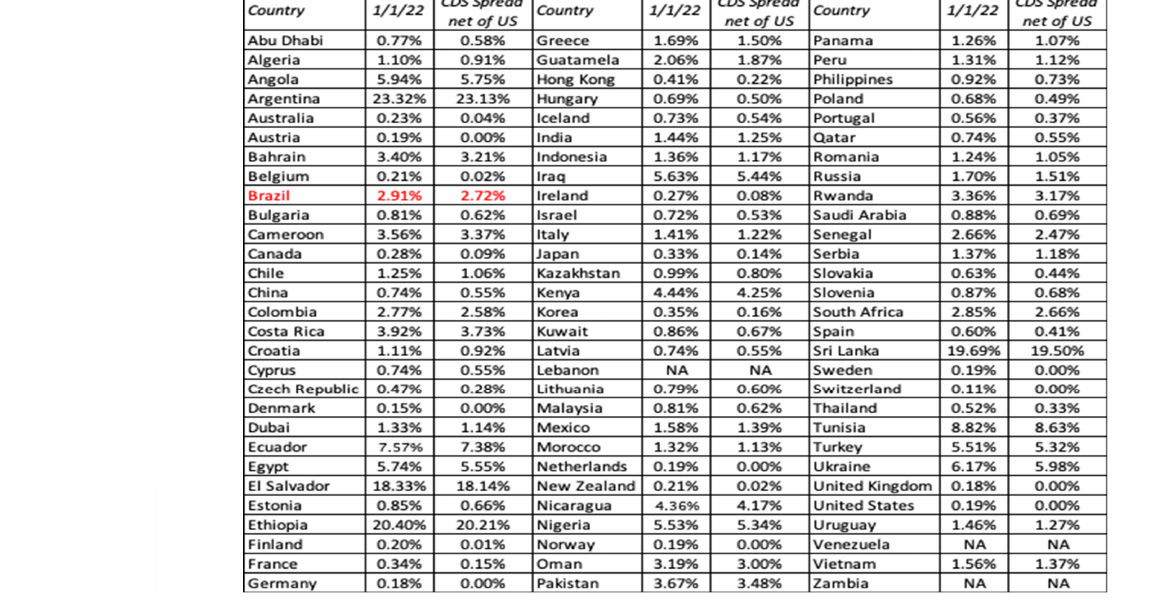
\includegraphics[width=0.85\textwidth]{L07_slide14.png}
\caption{CDS spreads by country, January 2022 (slide screenshot). Brazil: CDS 2.91\%, net of the US CDS 2.72\%.}
\end{figure}

\begin{exbox}[Test 3 (slide): risk-free rate in a currency -- Brazil]
The Brazilian government bond rate in nominal Reais on 1 January 2022 was 10.31\%. Three approaches to a nominal-Real $r_f$:
\begin{enumerate}
  \item \textbf{Government bond spread}: the 2032 USD-denominated Brazilian bond has a spread of 2.19\% over the US T-bond (3.70\% $-$ 1.51\%):\quad $r_f=10.31\%-2.19\%=\mathbf{8.12\%}$.
  \item \textbf{CDS spread}: Brazil's CDS spread net of the USD CDS spread was 2.72\%:\quad $r_f=10.31\%-2.72\%=\mathbf{7.59\%}$.
  \item \textbf{Rating-based spread}: Brazil had a Ba2 Moody's rating in LC; the spread for that class is 2.56\%:\quad $r_f=10.31\%-2.56\%=\mathbf{7.75\%}$.
\end{enumerate}
\end{exbox}

% =====================================================================
\section{Estimating the Equity Risk Premium (ERP)}

\subsection{Definitions}
\begin{itemize}
  \item \textbf{ERP}: the premium a \textbf{well-diversified marginal investor} requires to hold the market portfolio rather than a risk-free asset.
  \item \textbf{Historical ERP}: the premium stocks have \textbf{historically} earned over riskless securities over long periods. Implicit assumption: history can forecast the future.
  \item \textbf{Implied ERP}: the \textbf{forward-looking} premium implicitly priced in the \textbf{current} stock-market level, given expected aggregate cash flows and risk-free rates (see Martin, 2017, QJE). Implicit assumption: the market, overall and on average, is correctly priced.
\end{itemize}

\subsection{Peso Problems}
\begin{itemize}
  \item What about rare shocks? Also called \textbf{peso problems} or dark swans; very important for academics and practitioners.
  \item Answer: they account for \textbf{at most 1--2\%} of the historical equity premium. Not unimportant, and \textbf{insurable with index options}. Other long-run decline problems are harder to insure.
\end{itemize}

\subsection{Historical Risk Premium (HRP) Approach -- US}
Estimates are sensitive to:
\begin{enumerate}
  \item \textbf{Time period}: the ERP is time-varying; different periods give different measures; shorter periods have higher standard errors.
  \item \textbf{Choice of risk-free security}: T-bills (short term) vs T-bonds (long term). With an \textbf{upward-sloping} term structure, the ERP is \textbf{larger} when measured over short-term risk-free assets. Must be consistent with the $r_f$ used in the cost of capital.
  \item \textbf{Arithmetic vs geometric average}: \textbf{arithmetic} when returns are serially uncorrelated and the ERP estimate is for next year; \textbf{geometric} when returns are serially correlated (Fama--French 1988), adjusting for the long-term view (although we use 1-period models for the cost of capital).
\end{enumerate}
Even after the least-biased choices there are caveats:
\begin{enumerate}
  \item \textbf{Noisy estimates}: over 1928--2019 (about 90 years), with a 20\% annual standard deviation of returns, the standard error is $\geq2\%$:
  \[
  \text{Standard error in premium}\approx\frac{20\%}{\sqrt{90}}=2.1\%
  \]
  The implied standard deviation of equities rose to almost 50\% in the last quarter of 2008: think of the consequences for HRP if this volatility persisted.
  \item \textbf{Survivorship bias}: using 20th-century US data samples only the market that ``survived'' and was among the most successful.
\end{enumerate}
\begin{keybox}
There is a \textbf{trade-off between standard errors and survivorship bias}.
\end{keybox}
\begin{addbox}
Arithmetic $\geq$ geometric average always (e.g., returns $+50\%$, $-50\%$: arithmetic $0\%$, geometric $\sqrt{1.5\times0.5}-1=-13.4\%$). With 20 years instead of 90, the standard error would be $20\%/\sqrt{20}=4.5\%$, larger than the premium itself.
\end{addbox}

\subsection{HRP Approach -- Other Markets: Modified Historical Risk Premium}
\begin{keybox}[Modified historical risk premium]
\[
\text{ERP}=\text{Base premium for mature equity markets}+\text{Country premium}
\]
\end{keybox}
\begin{enumerate}
  \item \textbf{Base ERP} for a mature market: the US is the best available reference (4.72\% at end-2021).
  \item \textbf{Should there be a country premium?} Some argue country risk is fully diversifiable (open markets); Stulz (1999) argues it is not always diversifiable (segmented markets and/or cross-country correlation); Damodaran: add a \textbf{country risk premium (CRP)} when estimating the cost of capital for non-US markets.
  \item \textbf{How to estimate it?} Measure the \textbf{absolute country risk} and the firm's \textbf{exposure} to it.
\end{enumerate}

\subsection{CRP Approach 1: Default Risk Spreads}
CRP $=$ default spread of the bond issued by the country, but only if it is denominated in a currency for which a default-free entity exists. Two ways:
\begin{align*}
\text{(1)}\quad r_{e,USD}&=r_f+\beta\cdot\text{ERP}_{US}+\text{Default spread}\\
\text{(2)}\quad r_{e,USD}&=r_f+\beta\cdot(\text{ERP}_{US}+\text{Default spread})
\end{align*}
Shortcomings: (a) rating agencies lag markets in responding to changes in CRP; (b) a focus on default risk may obscure other risks for equity markets. Solutions: (a) use CDS spreads over a long period (e.g., 10 years); (b) use other risk measures: insurance prices, country scores (The Economist), or a CRP built up from fundamentals; (c) correct the default spread by the relative standard deviation.

\subsection{CRP Approach 2: Relative Standard Deviation}
The CRP is based on the volatility of market $X$ relative to the US market:
\[
\text{Relative SD}_X=\frac{\sigma_X}{\sigma_{US}}\qquad \text{ERP}_X=\text{ERP}_{US}\times\text{Relative SD}_X\qquad \text{CRP}_X=\text{ERP}_X-\text{ERP}_{US}
\]
Then use ERP$_X$ to estimate $r_e$. Shortcomings: (a) markets differ in structure and liquidity, which affects volatility; (b) some risky emerging markets have low volatility because of illiquidity; (c) currency differences (USD vs LC). Solutions: (a--b) examine the market structure and liquidity carefully; (c) compute USD-denominated returns to estimate the volatility of market $X$.

\subsection{CRP Approach 3: Default Spreads and Relative Standard Deviation}
\begin{keybox}
\[
\text{CRP}_X=\text{Country default spread}\times\frac{\sigma_{\text{Equity},X}}{\sigma_{\text{Bonds},X}}
\]
then (a) $r_{e,USD}=r_f+\beta\cdot\text{ERP}_{US}+\text{CRP}_X$ or (b) $r_{e,USD}=r_f+\beta\cdot(\text{ERP}_{US}+\text{CRP}_X)$.
\end{keybox}
Shortcomings and solutions are similar to the two previous approaches.
\begin{exbox}[Illustration (not on slides)]
Brazil: default spread 2.56\%, $\sigma_{\text{equity}}=30\%$, $\sigma_{\text{bonds}}=20\%$ $\Rightarrow$ CRP $=2.56\%\times1.5=3.84\%$. With $r_f=1.51\%$, ERP$_{US}=4.24\%$, $\beta=1.2$:\\
(a) $r_e=1.51\%+1.2\times4.24\%+3.84\%=10.44\%$; \quad (b) $r_e=1.51\%+1.2\times(4.24\%+3.84\%)=11.21\%$.\\
Relative-SD approach with $\sigma_{BR}/\sigma_{US}=1.6$: ERP$_{BR}=4.24\%\times1.6=6.78\%$, CRP $=2.54\%$.
\end{exbox}

\subsection{CRP: Exposure}
Three ways to bring the CRP into $r_e$, given the link between returns in LC and USD:
\[
r_{e,LC}=\left[(1+r_{e,USD})\cdot\frac{1+i_{LC}}{1+i_{USD}}\right]-1
\]
\begin{enumerate}
  \item \textbf{Every company in the country is equally exposed}: $r_{e,USD}=r_f+\beta\cdot\text{ERP}_{US}+\text{CRP}_{X}$ (implicit when using the local government's dollar borrowing rate as $r_f$).
  \item \textbf{Exposure to country risk $=$ exposure to market risk}: $r_{e,USD}=r_f+\beta\cdot(\text{ERP}_{US}+\text{CRP}_{X})$ (country risk is a portion of market risk).
  \item \textbf{Country risk as a separate factor}, firm-specific exposure $\lambda$: $r_{e,USD}=r_f+\beta\cdot\text{ERP}_{US}+\lambda\cdot\text{CRP}_{X}$ (multifactor model).
\end{enumerate}

\subsection{ERP Estimation Procedure and Implied ERP (January 2022)}

\begin{figure}[H]
\centering
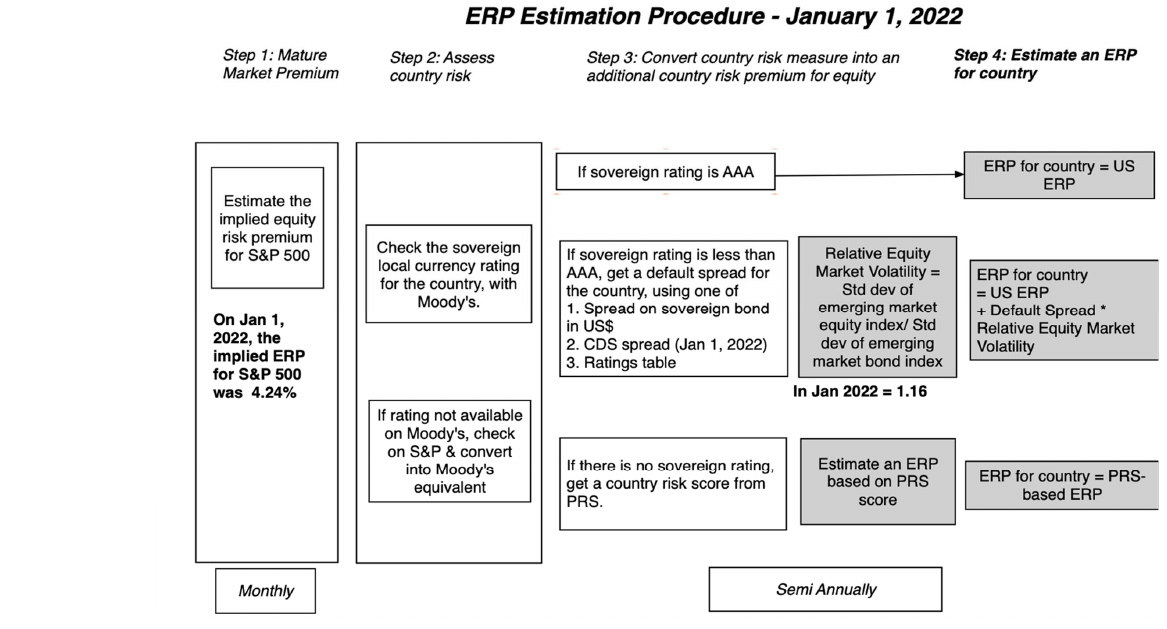
\includegraphics[width=0.9\textwidth]{L07_slide27.png}
\caption{ERP estimation procedure, 1 January 2022 (slide screenshot). Step 1: implied ERP for the S\&P 500 (4.24\%). Step 2: sovereign local-currency rating (Moody's; else S\&P or PRS score). Step 3: if the rating is below AAA, a default spread (sovereign \$ bond, CDS or ratings table) times the relative equity-market volatility (std dev of emerging-market equity index / std dev of emerging-market bond index $=1.16$ in January 2022). Step 4: ERP for the country $=$ US ERP $+$ default spread $\times$ relative equity-market volatility (or the PRS-based ERP).}
\end{figure}

\begin{figure}[H]
\centering
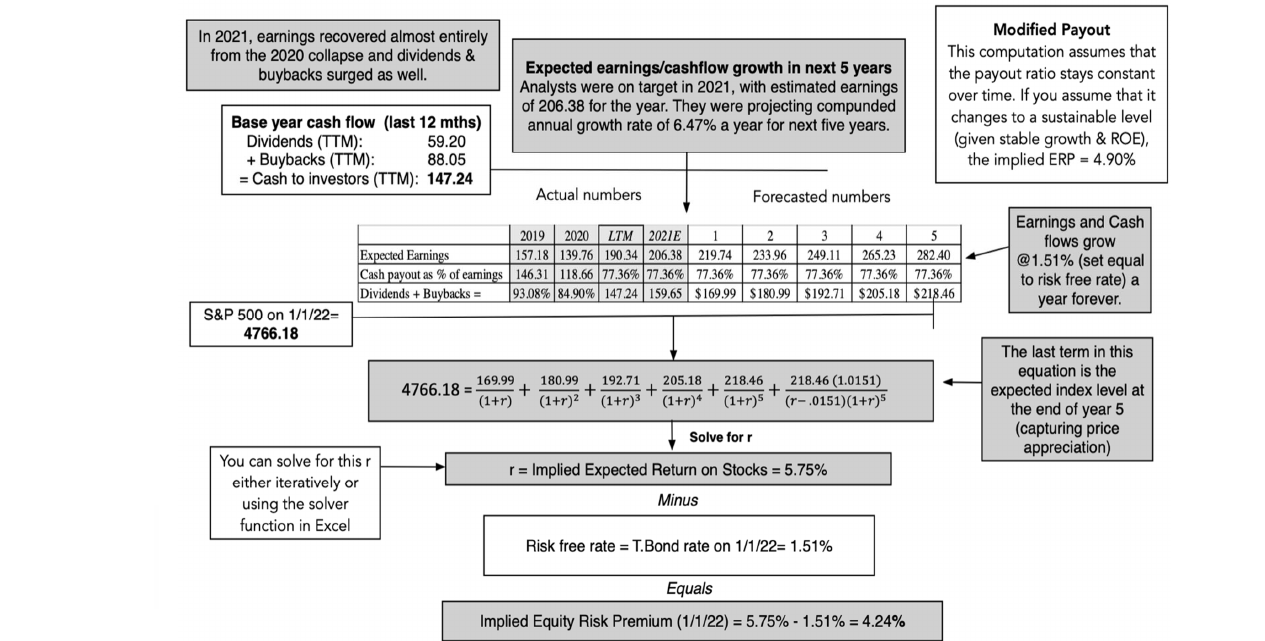
\includegraphics[width=0.9\textwidth]{L07_slide28.png}
\caption{Implied ERP, January 2022 (slide screenshot).}
\end{figure}

\begin{exbox}[Implied ERP: the computation step by step]
\begin{itemize}[leftmargin=*]
  \item Base-year cash to investors (last 12 months): dividends 59.20 + buybacks 88.05 $=$ \textbf{147.24}.
  \item Expected earnings grow at 6.47\% per year for 5 years (analysts); cash payout stays at 77.36\% of earnings $\Rightarrow$ cash flows: 169.99, 180.99, 192.71, 205.18, 218.46.
  \item After year 5, cash flows grow at 1.51\% ($=r_f$) forever.
  \item Solve for $r$ so that the index level equals the PV:
  \[
  4{,}766.18=\frac{169.99}{1+r}+\frac{180.99}{(1+r)^2}+\frac{192.71}{(1+r)^3}+\frac{205.18}{(1+r)^4}+\frac{218.46}{(1+r)^5}+\frac{218.46\times1.0151}{(r-0.0151)(1+r)^5}
  \]
  The last term is the expected index level at the end of year 5. Solution (iteratively or with Excel's solver): $r=\mathbf{5.75\%}$ (we verify: 5.753\%).
  \item Implied ERP $=5.75\%-1.51\%=\mathbf{4.24\%}$.
  \item \textbf{Modified payout}: if the payout moves to a sustainable level (given stable growth and ROE), the implied ERP $=4.90\%$.
\end{itemize}
\end{exbox}

\subsection{Part 1 Takeaways}
\begin{itemize}
  \item The CAPM is a model of how risk is priced in capital markets.
  \item In the CAPM, idiosyncratic risk can be diversified away $\Rightarrow$ \textbf{only systematic risk is priced}.
  \item The CAPM is empirically rejected, but it is still widely used to estimate the cost of equity. We need 3 parameters:
  \begin{itemize}
    \item \textbf{risk-free rate}, typically the yield of a long-term government bond;
    \item \textbf{beta}, from historical monthly, weekly or daily returns; estimates are noisy (use comparable companies to improve precision); measure it over a period in which leverage and operations are stable;
    \item \textbf{ERP}, the expected return on a broad-based index in excess of the risk-free rate.
  \end{itemize}
  \item The estimates of beta, ERP and risk-free rate are \textbf{logically linked together}.
\end{itemize}

% =====================================================================
\section*{PART 2 -- RISK PARAMETERS AND COST OF FINANCING}
\addcontentsline{toc}{section}{Part 2 -- Risk Parameters and Cost of Financing}

\section{Estimating Beta}

\subsection{Historical Market Betas}
Regress stock returns on market returns:
\begin{keybox}[Regression beta]
\[
r_{it}=\alpha+\beta\cdot r_{mt}+\varepsilon_{it},\qquad \beta=\frac{\text{Cov}(r_i,r_m)}{\text{Var}(r_m)}=\frac{\sigma_{im}}{\sigma_m^2}
\]
$\alpha$ = intercept; $\beta$ = slope: the riskiness of the stock relative to the market.
\end{keybox}
\textbf{Jensen's alpha.} To reconcile the CAPM with the regression:
\[
\mathbb{E}[r_i]=r_f+\beta\cdot\mathbb{E}[r_m-r_f]=r_f(1-\beta)+\beta\cdot\mathbb{E}[r_m]
\]
Compare the regression $\alpha$ (ex post) with $r_f(1-\beta)$ (ex ante):
\begin{center}
\begin{tabular}{@{}ll@{}}
\toprule
$\alpha>r_f(1-\beta)$ & the stock did \textbf{better} than expected over the period\\
$\alpha=r_f(1-\beta)$ & the stock did as expected\\
$\alpha<r_f(1-\beta)$ & the stock did \textbf{worse} than expected\\
\bottomrule
\end{tabular}
\end{center}
\begin{keybox}[Blume's adjustment (e.g., Bloomberg)]
\[
\beta_{\text{Adj}}=\beta_{\text{Raw}}\cdot\tfrac{2}{3}+1.00\cdot\tfrac{1}{3}
\]
(betas tend to revert towards 1 over time). Example: raw $\beta=1.6\Rightarrow\beta_{\text{Adj}}=1.067+0.333=1.40$.
\end{keybox}
Shortcomings: high standard errors; the regression reflects the firm's business mix and leverage \textbf{over the regression period}, not the current ones; not available for private firms and not reliable for illiquid markets.

\textbf{Summary of problems}
\begin{enumerate}
  \item \textbf{Historical returns}: a longer period gives more observations but may introduce biases from structural changes in the firm/industry risk profile $\Rightarrow$ use a shorter period, \textbf{between 2 and 5 years}.
  \item \textbf{Return type}: stock and market returns should include capital gains \textbf{and dividends}; some sources use price changes only.
  \item \textbf{Frequency}: daily returns give more observations but bias betas because of the illiquidity of some stocks.
  \item \textbf{Market index}: with internationally diversified investors, it is increasingly common to estimate $\beta$ against international indices (e.g., MSCI).
\end{enumerate}
\textbf{Solutions}
\begin{enumerate}
  \item Modify the regression beta: change the index, the frequency of returns, the length of the period; reduce the biases (Dimson 1979; Scholes and Williams 1977).
  \item \textbf{Accounting betas}: regress changes in the firm's earnings on changes in market earnings. Problems: (i) earnings smoothing, (ii) non-operating accounting policies, (iii) earnings frequency (at most quarterly).
  \item \textbf{Bottom-up beta (often preferable)}: requires understanding the type of business(es), the business mix and the financial leverage of the firm. The beta of a portfolio is the value-weighted average of the betas:
  \[
  \beta_P=\beta_a\omega_a+\beta_b\omega_b=\beta_a\frac{A}{A+B}+\beta_b\frac{B}{A+B}\iff \beta_P=\sum_{i=1}^{n}\beta_i\,\omega_i
  \]
\end{enumerate}

\subsection{Bottom-Up Betas: Determinants}
\begin{center}
\small
\begin{tabularx}{\textwidth}{@{}>{\raggedright\arraybackslash}p{3.6cm}>{\raggedright\arraybackslash}X>{\raggedright\arraybackslash}X@{}}
\toprule
\textbf{Determinant} & \textbf{Rule (other things equal)} & \textbf{Implications}\\
\midrule
\multicolumn{3}{@{}l}{\emph{Beta of the firm (unlevered $\beta$)}}\\
Nature of product/service & The more \textbf{discretionary} the product or service, the higher the $\beta$ & Cyclical $>$ non-cyclical; luxury $>$ basic goods; high-priced $>$ low-priced goods; growth firms have higher $\beta$\\
Operating leverage (fixed costs as \% of total costs) & The greater the proportion of \textbf{fixed costs}, the higher the $\beta$ & Rigid cost structures / high infrastructure needs $>$ flexible ones; small $>$ large firms; young $>$ mature firms\\
\midrule
\multicolumn{3}{@{}l}{\emph{Beta of equity (levered $\beta$)}}\\
Financial leverage & The greater the proportion of \textbf{debt}, the higher the equity $\beta$ & Highly levered firms have higher $\beta$; equity $\beta=$ unlevered $\beta\times$ (adjustment)\\
\bottomrule
\end{tabularx}
\end{center}

\subsection{Bottom-Up Betas: Ideal World and Real World}
\textbf{Ideal world}: start with the $\beta$ of the business the firm is in $\to$ adjust it for the operating leverage of the firm to obtain the unlevered $\beta$ $\to$ use the firm's financial leverage to obtain the levered (equity) $\beta$. Two alternatives (as in Chapter~\ref{ch:wacc}):
\begin{align*}
\text{Constant } D/(D+E):&\quad \beta_l=\beta_u\left[1+\frac{D}{E}\right]\\
\text{Fixed \$ debt (Hamada)}:&\quad \beta_l=\beta_u\left[1+(1-\tau_C)\frac{D}{E}\right]
\end{align*}

\textbf{Real world -- five steps}
\begin{enumerate}
  \item Find the business(es) your firm operates in.
  \item Find publicly traded firms in each business and obtain their regression $\beta$. \textbf{Unlever} each one with its own $D/E$: $\beta_u=\beta_{\text{regression}}/(1+D/E)$ [or Hamada if using APV]. Take the (simple or cap-weighted) average/median of these unlevered betas. Relever using your firm's $D/E$ (for pure players only). \emph{Refinement}: adjust for differences in operating leverage and product characteristics between your firm and the comparables.
  \item Estimate how much value your firm derives from each business. \emph{Refinement}: revenues or operating income are often used as weights, but it is better to estimate the \textbf{value} of each business.
  \item Compute the weighted average of the unlevered betas of the businesses (step 2) with the weights of step 3: \textbf{bottom-up unlevered $\beta$}. \emph{Refinement}: if the business mix changes over time, change the weights year by year.
  \item Compute the levered (equity) $\beta$ with the firm's \textbf{market} $D/E$: $\beta_l=\beta_u(1+D/E)$ [or Hamada if using APV] (if debt is riskless). \emph{Refinement}: if $D/E$ is expected to change, the levered $\beta$ changes over time.
\end{enumerate}

\begin{exbox}[Illustration (not on slides): bottom-up beta of a two-business firm]
Business A: comparables' average regression $\beta=1.20$, average $D/E=0.50$ $\Rightarrow\beta_u=1.20/1.5=0.80$. Business B: $\beta=0.90$, $D/E=0.20\Rightarrow\beta_u=0.75$.\\
Value weights: A 60\%, B 40\% $\Rightarrow\beta_u=0.6\times0.80+0.4\times0.75=0.78$.\\
Firm's market $D/E=0.40$: $\beta_l=0.78\times1.40=\mathbf{1.092}$ (textbook) or, with $\tau=25\%$, Hamada $0.78\times(1+0.75\times0.4)=\mathbf{1.014}$.
\end{exbox}

\subsection{Bottom-Up Betas: Adjusting Financial Leverage}
\begin{keybox}[Three approaches]
\textbf{1. Hamada} ($\beta_D=0$, $D$ fixed in \$): \quad $\beta_L=\beta_U\left[1+(1-\tau_C)\frac{D}{E}\right]$\\[4pt]
\textbf{2. Textbook WACC} ($D/E$ fixed, $\beta_D=0$): \quad $\beta_L=\beta_U\left[1+\frac{D}{E}\right]$\\[4pt]
\textbf{3. Debt-adjusted} (debt carries market risk, $\beta_D\neq0$):
\begin{align*}
\beta_L&=\beta_U\left[1+(1-\tau_C)\frac{D}{E}\right]-\beta_D(1-\tau_C)\frac{D}{E}\quad\text{(\$ debt fixed)}\\
\beta_L&=\beta_U\left[1+\frac{D}{E}\right]-\beta_D\frac{D}{E}\quad(D/E\text{ fixed})
\end{align*}
\end{keybox}
While the debt-adjusted approach is desirable, \textbf{estimating $\beta_D$ is often challenging}.

\subsection{Bottom-Up Betas: Reasons to Use Them}
\begin{itemize}
  \item \textbf{Lower noise}: the standard error of a bottom-up $\beta$ is much lower than that of a single regression $\beta$:
  \[
  \text{Std error of bottom-up }\beta\approx\frac{\text{Average std error across }\beta\text{s}}{\sqrt{\#\text{ of firms in sample}}}
  \]
  e.g., average error 0.25 with 25 comparables $\Rightarrow0.25/5=0.05$.
  \item \textbf{Current operating structure}: can be adjusted to changes in business mix and leverage; the regression $\beta$ reflects the past.
  \item \textbf{Financial structure}: can reflect recent or future changes (e.g., restructuring).
  \item \textbf{Private firms, illiquid stocks, start-ups}: can be estimated without historical prices (IPOs, divisions, start-ups).
\end{itemize}

% =====================================================================
\section{Estimating Lambda ($\lambda$)}

\subsection{Determinants}
If country risk is a separate factor with firm-specific exposures:
\[
r_{e,USD}=r_{f,USD}+\beta\cdot\text{ERP}_{US}+\lambda_{\text{firm},X}\cdot\text{CRP}_{X,USD},\qquad r_{e,LC}=\left[(1+r_{e,USD})\cdot\frac{1+i_{LC}}{1+i_{USD}}\right]-1
\]
\begin{itemize}
  \item \textbf{Source of revenues}: the more revenues a firm generates in a country, the more exposed it is (a Brazilian firm selling mostly in Brazil is more exposed than one selling mostly abroad).
  \item \textbf{Manufacturing facilities}: a firm with all its production in the country is more exposed; the problem is amplified for firms that cannot move their facilities (mining, oil).
  \item \textbf{Use of risk management}: options/futures, insurance and real investment can hedge country risk.
\end{itemize}

\subsection{Approaches}
\begin{enumerate}
  \item \textbf{Revenue breakdown} (easiest data): the proportion of revenues generated in the country, scaled by that of the average firm in the country:
  \[
  \lambda_{\text{firm},X}=\frac{\%\text{ of revenues in country }X_{\text{firm}}}{\%\text{ of domestic revenues}_{\text{average firm in country }X}}
  \]
  \item \textbf{Regression vs the country bond}: regress the firm's stock returns on the returns of the country bond (country-bond returns are assumed to be a function of country risk):
  \[
  r_{e,\text{firm}}=\alpha+\lambda_{\text{firm},X}\cdot r_{d,X}+\varepsilon,\qquad \lambda_{\text{firm},X}=\frac{\text{Cov}(r_{e,\text{firm}},r_{d,X})}{\text{Var}(r_{d,X})}
  \]
\end{enumerate}
\begin{exbox}[Illustration (not on slides)]
A Brazilian firm earns 35\% of its revenues in Brazil; the average Brazilian firm earns 70\% domestically $\Rightarrow\lambda=0.35/0.70=0.5$. With $r_f=1.51\%$, $\beta=1.1$, ERP$_{US}=4.24\%$, CRP $=3.84\%$: $r_{e,USD}=1.51\%+1.1\times4.24\%+0.5\times3.84\%=8.09\%$.\\
In Reais with $i_{BR}=6\%$, $i_{US}=2\%$: $r_{e,BRL}=1.0809\times\frac{1.06}{1.02}-1=12.33\%$.
\end{exbox}

% =====================================================================
\section{The Cost of Equity: Recap}

\begin{keybox}[Cost of equity]
\[
r_{e,USD}=r_{f,USD}+\beta\cdot\text{ERP}_{US}+\lambda_X\cdot\text{CRP}_{X,USD}
\]
\begin{itemize}[leftmargin=*]
  \item \textbf{Market risk exposure ($\beta$)}: (1) regression $\beta$; (2) accounting $\beta$; (3) \textbf{bottom-up $\beta$ (preferred)}: based on other firms in the business and the firm's own financial leverage.
  \item \textbf{Country risk exposure ($\lambda$)}: (1) $\lambda=1$; (2) $\lambda=\beta$; (3) $\lambda$ estimated specifically.
  \item \textbf{Risk-free rate}: has to be ``fully'' risk-free; in the same \textbf{currency} as the cash flows; in the same \textbf{terms} (real or nominal) as the cash flows.
  \item \textbf{Historical premium}: (1) mature-market premium: average premium of stocks over T-bonds in the US; (2) country risk premium: default spread, relative standard deviation, or default spread $\times$ relative standard deviation.
  \item \textbf{or Implied premium}: based on (i) how the equity market is priced today and (ii) a simple PV model from which the implied premium is backed out.
\end{itemize}
\end{keybox}

% =====================================================================
\section{The Cost of Debt: Recap}

\subsection{Determinants}
The cost of debt $r_D$ is the rate at which a firm can borrow, for a given maturity.
\begin{itemize}
  \item Promised interest rate (promised yield) $\neq$ expected interest rate.
  \item \textbf{Promised rate $=$ time premium $+$ default premium}.
  \item \textbf{Expected rate $=$ time premium} $\Leftarrow$ $r_D<$ promised yield.
\end{itemize}
Determinants:
\begin{enumerate}
  \item \textbf{Risk-free rate}: as it rises, the cost of debt rises.
  \item \textbf{Default risk of the company}: as the default spread rises, the cost of debt rises. It is related to country risk too (e.g., the cost of debt of Italian companies in 2011), but not all companies have equal country-risk exposure.
  \item \textbf{Tax shield}: interest is tax deductible $\Rightarrow$ the after-tax cost of debt depends on the \textbf{marginal} corporate tax rate:
  \[
  \text{After-tax cost of debt}=\text{Pre-tax cost of debt}\times(1-\tau_C)
  \]
\end{enumerate}

\subsection{Approaches}
\begin{enumerate}
  \item \textbf{Recent borrowing history}: yield to maturity on a liquid straight bond of the same firm. Limitation: very few firms have liquid, traded long-term straight bonds.
  \item \textbf{Public rating}: estimate a default spread from the firm's rating. More robust, but different bonds of the same firm can have different ratings $\Rightarrow$ use the median rating.
  \item \textbf{Synthetic rating}: if the firm has no rating or multiple ratings, estimate a synthetic rating from the interest coverage ratio, $\text{ICR}=\text{EBIT}/\text{Interest expenses}$ (other models exist, e.g., Altman's Z-score), as in the Disney case (Chapter~\ref{ch:capstr}).
\end{enumerate}
\textbf{Cost of debt as an IRR.} We only observe the promised yield (YTM), not $r_D$; estimate $r_D$ as the IRR of the \textbf{expected} cash flows and the current price:
\[
\frac{\mathbb{E}_0[CF_1]}{1+r_D}+\frac{\mathbb{E}_0[CF_2]}{(1+r_D)^2}+\dots+\frac{\mathbb{E}_0[CF_T]}{(1+r_D)^T}-\text{Price}_0=0
\]
\textbf{General rule}: (promised) YTM $\geq$ cost of debt; strict iff there is any probability of default with recovery below 100\%; the gap grows with the default probability; \textbf{YTM $-$ cost of debt $=$ expected default loss} (numerical example in Chapter~\ref{ch:capstr}).

% =====================================================================
\section{WACC: Weights and Recap}

\subsection{Weights for Computation}
\begin{keybox}[General rule]
Use \textbf{market-value weights}, not book values: the cost of capital measures the cost of issuing securities, which are issued at market value.
\end{keybox}
\begin{itemize}
  \item \textbf{Debt} (net of cash \& equivalents):
  \begin{itemize}
    \item only \textbf{interest-bearing} debt, not all liabilities (exclude trade payables, \dots), both short and long term;
    \item capitalize the PV of future operating-lease payments (off-balance-sheet debt);
    \item estimate the market value of non-traded debt as a bond:
    \[
    D_{\text{Market value}}=\text{Coupon}\cdot\frac{1}{r_d}\left[1-\frac{1}{(1+r_d)^t}\right]+\frac{\text{Face value}}{(1+r_d)^t}
    \]
    (coupon $=$ interest expense; $t$ $=$ average maturity);
    \item modify the interest coverage ratio for the synthetic rating when leases are capitalized:
    \[
    \text{Modified ICR}=\frac{\text{EBIT}+\text{Operating lease expenses}}{\text{Interest expenses}+\text{Implicit interest on leases}}
    \]
  \end{itemize}
  \item \textbf{Equity}: current price $\times$ number of shares outstanding; for private firms use comparables' multiples. Include \textbf{all equity claims} (minorities, warrants, management stock options, \dots).
  \item \textbf{Hybrid securities}: include their market value (and required return).
\end{itemize}
\begin{exbox}[Illustration (not on slides): market value of book debt]
Book debt 1,000, interest expense 50, average maturity 6 years, current pre-tax $k_d=7\%$:
\[
D_{MV}=50\times\frac{1-1.07^{-6}}{0.07}+\frac{1{,}000}{1.07^{6}}=50\times4.7665+666.34=238.33+666.34=\mathbf{904.7}
\]
Debt issued at 5\% is worth less than book value when rates rise to 7\%.
\end{exbox}

\subsection{WACC Recap}
\begin{center}
\begin{tikzpicture}[b/.style={draw=navy,fill=white,rounded corners=2pt,text width=4.2cm,align=left,font=\scriptsize,inner sep=4pt}]
\node[draw=navy,thick,fill=boxblue,inner sep=6pt] (w) at (0,0) {$\displaystyle \text{WACC}=r_d(1-t_c)\frac{D}{D+E+S}+r_e\frac{E}{D+E+S}+r_s\frac{S}{D+E+S}$};
\node[b] (t) at (-3.5,2.1) {\textbf{Tax rate}: marginal tax rate, reflecting the tax benefits of debt};
\node[b] (m) at (3.5,2.1) {\textbf{Market values}: 1.\ Debt; 2.\ Equity; 3.\ Hybrid securities};
\node[b] (d) at (-5,-2.1) {\textbf{Cost of debt ($r_d$)} based on: current cost of borrowing; synthetic rating};
\node[b] (e) at (0,-2.1) {\textbf{Cost of equity ($r_e$)}: CAPM with $r_f$, $\beta$, ERP, $\lambda\cdot$CRP};
\node[b] (s) at (5,-2.1) {\textbf{Cost of hybrids ($r_s$)}: must reflect expected payments and current market values};
\foreach \x in {t,m,d,e,s} \draw[navy] (\x) -- (w);
\end{tikzpicture}
\end{center}

\section{Takeaways (Part 2)}
\begin{itemize}
  \item In general, \textbf{cost of debt $k_d\leq$ promised yield}, with equality iff the default probability is zero. Methods to estimate $k_d$:
  \begin{itemize}
    \item equate the PV of expected cash flows to the current debt value and solve for the IRR;
    \item use a CAPM approach that adds a risk premium to AA yields as a function of rating class;
    \item use credit default swaps as a guide;
    \item if everything else fails, use comparables and their cost of debt.
  \end{itemize}
  \item The WACC is used to value the firm when it operates with a \textbf{fixed leverage} $D/(D+E)$.
  \item Financial distress costs and agency costs are \textbf{countervailing forces} to the tax advantages of debt.
\end{itemize}

% =====================================================================
\section{Formula Summary Sheet}
\begin{center}
\small
\renewcommand{\arraystretch}{1.45}
\begin{longtable}{@{}p{4.8cm}p{10.2cm}@{}}
\toprule
\textbf{Concept} & \textbf{Formula}\\
\midrule
\endhead
DCF value & $V_t=\sum_{s}\mathbb{E}_t[\text{FCF}_s]/(1+r)^{s-t}$\\
WACC (3 securities) & $r_d(1-\tau)\frac{D}{V}+r_e\frac{E}{V}+r_s\frac{S}{V}$, $V=D+E+S$ (market values)\\
CAPM & $\mathbb{E}[r_e]=r_f+\beta(\mathbb{E}[r_m]-r_f)$\\
Multifactor & $\mathbb{E}[r_e]=r_f+\sum_i\beta_i\,\mathbb{E}[r_i-r_f]$\\
Real rate & $r_{\text{real}}=\frac{1+r_{\text{nom}}}{1+i}-1\approx r_{\text{nom}}-i$\\
$r_f$ in local currency & Govt bond (LC) $-$ default spread (or $-$ CDS spread)\\
Build-up $r_f$ & Expected inflation $+$ expected long-term real growth\\
Covered interest parity & $F_{LC,USD}=S_{LC,USD}\times\frac{1+r_{f,LC}}{1+r_{f,USD}}$\\
Uncovered (inflation) parity & $(1+r_{f,USD})=(1+r_{f,LC})\frac{1+i_{USD}}{1+i_{LC}}$\\
Std error of ERP & $\sigma/\sqrt{T}$ (20\%/$\sqrt{90}$ = 2.1\%)\\
Modified HRP & ERP $=$ mature-market premium $+$ CRP\\
CRP (relative SD) & ERP$_X=$ ERP$_{US}\times\sigma_X/\sigma_{US}$;\ CRP $=$ ERP$_X-$ ERP$_{US}$\\
CRP (spread $\times$ rel.\ vol.) & CRP $=$ default spread $\times\sigma_{\text{equity},X}/\sigma_{\text{bonds},X}$\\
Cost of equity with CRP & $r_f+\beta\,\text{ERP}+\text{CRP}$;\ $r_f+\beta(\text{ERP}+\text{CRP})$;\ $r_f+\beta\,\text{ERP}+\lambda\,\text{CRP}$\\
USD $\to$ LC cost of equity & $r_{e,LC}=(1+r_{e,USD})\frac{1+i_{LC}}{1+i_{USD}}-1$\\
Implied ERP & solve $P_0=\sum CF_t/(1+r)^t+\frac{CF_5(1+g)}{(r-g)(1+r)^5}$;\ ERP $=r-r_f$\\
Regression beta & $\beta=\text{Cov}(r_i,r_m)/\text{Var}(r_m)$\\
Jensen's alpha & compare $\alpha$ with $r_f(1-\beta)$\\
Blume adjustment & $\beta_{\text{adj}}=\frac23\beta_{\text{raw}}+\frac13$\\
Portfolio beta & $\beta_P=\sum_i\beta_i\omega_i$ (value weights)\\
Unlever / relever & $\beta_u=\beta_l/(1+D/E)$;\ Hamada $\beta_l=\beta_u[1+(1-\tau)D/E]$\\
Debt-adjusted beta & $\beta_L=\beta_U[1+(1-\tau)\frac{D}{E}]-\beta_D(1-\tau)\frac{D}{E}$;\ or $\beta_U(1+\frac{D}{E})-\beta_D\frac{D}{E}$\\
Std error of bottom-up $\beta$ & average std error / $\sqrt{n}$\\
Lambda (revenues) & \% revenues in $X$ (firm) / \% domestic revenues (average firm in $X$)\\
Lambda (regression) & $\lambda=\text{Cov}(r_e,r_{d,X})/\text{Var}(r_{d,X})$\\
Promised vs expected rate & promised $=$ time $+$ default premium;\ expected $=$ time premium\\
After-tax cost of debt & $k_d(1-\tau_{\text{marginal}})$\\
Interest coverage & EBIT / interest expenses\\
Modified ICR (leases) & (EBIT $+$ lease exp.) / (interest $+$ implicit lease interest)\\
Market value of debt & Coupon$\cdot\frac{1-(1+r_d)^{-t}}{r_d}+\frac{\text{Face}}{(1+r_d)^t}$\\
YTM vs $k_d$ & YTM $-k_d=$ expected default loss\\
\bottomrule
\end{longtable}
\end{center}

\needspace{14\baselineskip}
\section{Common Mistakes and Exam Traps}
\begin{trapbox}[Exam traps -- Chapter 7]
\begin{enumerate}[leftmargin=*]
  \item A risk-free asset has \textbf{no default risk and no reinvestment risk}; not all government bonds are risk-free.
  \item \textbf{Consistency}: currency of $r_f$ $=$ currency of cash flows; nominal with nominal, real with real; match maturities.
  \item $r_{\text{real}}\approx r_{\text{nom}}-i$ only for \textbf{low} inflation; exact $(1+r)/(1+i)-1$.
  \item $r_f$ in LC $=$ local govt bond rate \textbf{minus} the default (or CDS) spread. Brazil: 8.12\% (bond spread), 7.59\% (CDS), 7.75\% (rating).
  \item Historical ERP: arithmetic average for 1-year horizon with uncorrelated returns; geometric for serially correlated returns / long horizon. An upward-sloping term structure makes the ERP over T-bills \textbf{larger} than over T-bonds.
  \item Std error of a 90-year ERP $\approx20\%/\sqrt{90}=2.1\%$; trade-off between standard error and survivorship bias.
  \item Peso problems explain at most 1--2\% of the historical premium.
  \item Implied ERP assumes the market is correctly priced; historical ERP assumes history predicts the future. Jan 2022: implied return 5.75\%, ERP $5.75\%-1.51\%=$ \textbf{4.24\%} (4.90\% with modified payout).
  \item Three CRP approaches: default spread; relative standard deviation ($\sigma_X/\sigma_{US}$); default spread $\times\sigma_{\text{equity}}/\sigma_{\text{bond}}$.
  \item Three exposure assumptions: all firms equally exposed (add CRP); exposure $=\beta$ (CRP inside the bracket); separate factor $\lambda$.
  \item $\beta=\text{Cov}/\text{Var}$ (not Cov/$\sigma_i\sigma_m$, which is the correlation). Jensen's $\alpha$ is compared with $r_f(1-\beta)$, not with zero.
  \item Blume: $\frac23\beta_{\text{raw}}+\frac13$ (betas move toward 1).
  \item Regression beta: 2--5 years; returns including dividends; daily data biased by illiquidity; regression beta reflects past mix and leverage.
  \item Bottom-up: unlever comparables with \textbf{their own} $D/E$, average, weight by \textbf{value} of each business, relever with the \textbf{firm's market} $D/E$. Lower standard error ($\div\sqrt{n}$).
  \item Unlevered $\beta$ is driven by discretionary products and operating leverage; levered $\beta$ adds financial leverage. Cyclical, luxury, small, young, growth firms have higher $\beta$.
  \item $\lambda$: revenue share in the country relative to the average domestic firm; or regression on country-bond returns.
  \item Promised yield $=$ time $+$ default premium; the cost of debt is the expected return (time premium only).
  \item WACC weights: market values; only \textbf{interest-bearing} debt (net of cash), plus capitalized leases; all equity claims; hybrids at market value.
  \item The WACC presumes a \textbf{fixed leverage ratio} $D/(D+E)$.
\end{enumerate}
\end{trapbox}

\chapter{Growth and Value}\label{ch:growth}

\emph{Based on Lecture L08 (34 slides): ``Growth \& Value''. Workflow step: forecasts and cash flows $\to$ \textbf{terminal value}.}

% =====================================================================
\section{Estimating Growth}

\subsection{Definition and Approaches}

\begin{center}
\small
\begin{tabular}{@{}lp{5.2cm}|ll@{}}
\multicolumn{2}{c|}{\textbf{Assets}} & \multicolumn{2}{c}{\textbf{Liabilities}}\\
\midrule
\textbf{Assets in place} & Existing investments: generate cash flows \textbf{today} & (Net) Debt & Borrowed money\\
\textbf{Growth opportunities} & Investments to be made: generate cash flows \textbf{tomorrow} & Equity & Owners' funds\\
\end{tabular}
\end{center}
Value of the firm (equity or asset side) with the DCF approach:
\begin{keybox}[DCF with terminal value]
\[
\text{Value}_0=\sum_{t=1}^{n}\frac{\mathbb{E}[CF_t]}{(1+k_c)^t}+\frac{\text{Terminal Value}_n}{(1+k_c)^n},\qquad\text{under stable growth } \text{TV}_n=\frac{\mathbb{E}[CF_{n+1}]}{k_c-g}
\]
$CF_t$: expected cash flow (equity or asset side); $k_c$: cost of capital (equity or asset side); $g$: long-run growth of CF.
\end{keybox}
Three main approaches to estimate $g$:
\begin{enumerate}
  \item \textbf{Historical}: based on historical growth in EPS.
  \item \textbf{Analysts' estimates}: based on analysts' estimates of EPS growth.
  \item \textbf{Fundamental}: based on the fundamentals of EPS growth: \textbf{reinvestment} (non-cash WC and net CapEx) and \textbf{return on investment} (the returns those projects earn).
\end{enumerate}

\subsection{Historical Approach}
\begin{keybox}[Ways to measure historical growth]
\begin{enumerate}[leftmargin=*]
  \item \textbf{Arithmetic average}: \ $g_t=\frac1n\sum_{i=1}^{n}g_{t-i}=\frac1n\sum_{i=1}^{n}\frac{NI_{t-i}-NI_{t-i-1}}{NI_{t-i-1}}$
  \item \textbf{Geometric average}: \ $g_t=\left[\prod_{i=1}^{n}(1+g_{t-i})\right]^{1/n}-1=\left(\frac{NI_t}{NI_{t-n}}\right)^{1/n}-1$
  \item \textbf{Log-linear OLS regression}: $\ln(\text{EPS})=a+b\cdot t$; $\hat b$ is the percentage change in EPS per unit of time.
  \item \textbf{Time-series models} (Box and Jenkins 1976; Foster 1977; Griffin 1977).
\end{enumerate}
\end{keybox}
Historical rates are sensitive to:
\begin{enumerate}
  \item the \textbf{estimation period} (to be chosen carefully, especially for young/high-growth firms);
  \item \textbf{negative earnings}: if some EPS are negative, $\ln(\text{EPS})$ cannot be computed for the log-linear regression;
  \item \textbf{earnings volatility}, high especially for young/high-growth industries. Revenue growth is more stable and more serially correlated than earnings growth, so it is a useful check;
  \item \textbf{size effect}: growth is ``convex'': it falls as size increases;
  \item changes in EPS not driven by earnings (e.g., stock splits).
\end{enumerate}

\begin{exbox}[Historical approach: Motorola (\$ million) -- verified]
\small
\begin{minipage}[t]{0.48\linewidth}
\begin{tabular}{@{}lrr@{}}
\toprule
Year & Revenues & \% change\\
\midrule
X & 22,245 & \\
X+1 & 27,037 & 21.54\%\\
X+2 & 27,973 & 3.46\%\\
X+3 & 29,794 & 6.51\%\\
X+4 & 29,398 & $-1.33\%$\\
X+5 & 30,931 & 5.21\%\\
\midrule
\multicolumn{2}{@{}l}{Arithmetic average} & 7.08\%\\
\multicolumn{2}{@{}l}{Geometric average} & 6.82\%\\
\multicolumn{2}{@{}l}{Standard deviation} & 8.61\%\\
\bottomrule
\end{tabular}

\medskip
\begin{tabular}{@{}lrr@{}}
\toprule
Year & EBIT & \% change\\
\midrule
X & 2,604 & \\
X+1 & 2,931 & 12.56\%\\
X+2 & 1,960 & $-33.13\%$\\
X+3 & 1,947 & $-0.66\%$\\
X+4 & 822 & $-57.78\%$\\
X+5 & 3,216 & 291.24\%\\
\midrule
\multicolumn{2}{@{}l}{Arithmetic average} & 42.45\%\\
\multicolumn{2}{@{}l}{Geometric average} & 4.31\%\\
\multicolumn{2}{@{}l}{Standard deviation} & 141.78\%\\
\bottomrule
\end{tabular}
\end{minipage}\hfill
\begin{minipage}[t]{0.48\linewidth}
\begin{tabular}{@{}lrr@{}}
\toprule
Year & EBITDA & \% change\\
\midrule
X & 4,151 & \\
X+1 & 4,850 & 16.84\%\\
X+2 & 4,268 & $-12.00\%$\\
X+3 & 4,276 & 0.19\%\\
X+4 & 3,019 & $-29.40\%$\\
X+5 & 5,398 & 78.80\%\\
\midrule
\multicolumn{2}{@{}l}{Arithmetic average} & 10.89\%\\
\multicolumn{2}{@{}l}{Geometric average} & 5.39\%\\
\multicolumn{2}{@{}l}{Standard deviation} & 41.56\%\\
\bottomrule
\end{tabular}

\medskip
\begin{tabular}{@{}lrr@{}}
\toprule
Year & EPS & \% change\\
\midrule
X & 0.88 & \\
X+1 & 0.98 & 11.36\%\\
X+2 & 0.65 & $-33.67\%$\\
X+3 & 0.66 & 1.54\%\\
X+4 & 0.14 & $-78.79\%$\\
X+5 & 0.45 & 221.43\%\\
\midrule
\multicolumn{2}{@{}l}{Arithmetic average} & 24.37\%\\
\multicolumn{2}{@{}l}{Geometric average} & $-12.55\%$\\
\multicolumn{2}{@{}l}{Standard deviation} & 115.69\%\\
\bottomrule
\end{tabular}
\end{minipage}

\medskip
\textbf{How to compute (e.g., revenues):} arithmetic $=(21.54+3.46+6.51-1.33+5.21)/5=7.08\%$; geometric $=(30{,}931/22{,}245)^{1/5}-1=1.3905^{0.2}-1=6.82\%$.
\end{exbox}
\begin{addbox}[Lesson of the Motorola table]
The further down the income statement, the more volatile growth becomes (SD 8.6\% for revenues vs 141.8\% for EBIT). With volatile data the arithmetic average is badly inflated by one large rebound: EBIT +42.45\% arithmetic vs +4.31\% geometric; EPS +24.37\% arithmetic vs $-12.55\%$ geometric (EPS actually fell from 0.88 to 0.45). Use the geometric average and check against revenue growth.
\end{addbox}

\subsection{Analysts' Estimates Approach}
\begin{itemize}
  \item Consensus growth estimates are available from online providers (e.g., I/B/E/S).
  \item Analysts forecast EPS based on: (1) historical growth; (2) public information other than earnings affecting EPS growth; (3) recent firm-specific information updating the historical estimate; (4) recent market/industry information; (5) information revealed by competitors and/or private information.
  \item Estimates are sensitive to: (1) the number of analysts covering the firm (increasing in market cap, institutional holdings and trading volume); (2) the extent of disagreement; (3) the independence of estimates; (4) analysts' quality.
\end{itemize}
\textbf{Analysts' five ``deadly sins''}:
\begin{enumerate}[label=(\roman*)]
  \item \textbf{Tunnel vision}: too focused on the industry.
  \item \textbf{``Lemmingitis''} (herding): the urge to revise when others do, in the same direction and magnitude.
  \item \textbf{Stockholm syndrome}: identification with the managers.
  \item \textbf{Factophobia}: relying on ``stories'' rather than facts.
  \item \textbf{Dr.\ Jekyll/Mr.\ Hyde}: bringing business to investment banks.
\end{enumerate}

\subsection{Fundamentals' Approach I: EPS Growth}
The fundamentals' approach estimates growth as an \textbf{endogenous} variable.
\begin{keybox}[EPS growth]
\[
g=\text{Retention ratio}\ (b)\times\text{ROE}
\]
\end{keybox}
\textbf{Proof.} Define $g=\frac{NI_t-NI_{t-1}}{NI_{t-1}}$ and $\text{ROE}_{t-1}=\frac{NI_{t-1}}{BV_{t-2}}$ (BV $=$ book value of equity). With no equity injections, $NI_t=BV_{t-1}\times\text{ROE}_t=(BV_{t-2}+\text{Retained earnings}_{t-1})\times\text{ROE}_t$. With constant ROE:
\[
NI_t-NI_{t-1}=\text{RE}_{t-1}\times\text{ROE}\ \Rightarrow\ g=\frac{\text{Retained earnings}_{t-1}}{NI_{t-1}}\times\text{ROE}=b\times\text{ROE}.\qquad\text{QED}
\]
Implicit assumptions: constant ROE; no equity issuance (so NI growth $=$ EPS growth); no other comprehensive income in book equity.

\subsection{Fundamentals' Approach II: Net Income Growth}
\begin{keybox}[NI growth with the equity reinvestment rate]
\[
\text{Equity reinvested}_t=(\text{CapEx}_t-\text{D\&A}_t)+\Delta\text{WC}_t-(\text{New debt issued}_t-\text{Debt repaid}_t)
\]
\[
b_t=\frac{\text{Equity reinvested}_t}{NI_t}\qquad\qquad g_{t+1}=b_t\times\text{ROE}
\]
\end{keybox}
Adjust all figures (R\&D, operating leases, etc.) consistently with the adjustments made to cash flows. Implicit assumptions: constant ROE; \textbf{equity issuance allowed}, so NI growth $\neq$ EPS growth; no OCI in book equity.

\subsection{Fundamentals' Approach: ROE and Leverage}
Following Modigliani--Miller (with taxes):
\[
k_A=k_E\frac{E}{D+E}+k_D(1-\tau_C)\frac{D}{D+E}\iff k_E=k_A+[k_A-k_D(1-\tau_C)]\frac{D}{E}
\]
\begin{keybox}[Accounting version]
\[
\text{ROE}=\text{ROC}+[\text{ROC}-i(1-\tau_C)]\frac{D}{E}
\]
\vspace{-6pt}
\begin{gather*}
\text{ROC}=\frac{\text{EBIT}(1-\tau_C)}{\text{BV debt}-\text{Cash}+\text{BV equity}}=\frac{\text{EBIT}(1-\tau_C)}{\text{BV net debt}+\text{BV equity}}\\
\frac{D}{E}=\frac{\text{BV net debt}}{\text{BV equity}}\qquad i=\frac{\text{Interest expenses on (net) debt}}{\text{BV of (net) debt}}
\end{gather*}
\end{keybox}
Implications: ROE depends on the returns on investments undertaken (ROC); \textbf{ROE changes with leverage} (and financial risk); the higher the cost of debt, the lower the ROE; marginal ROE differs from average ROE $\Rightarrow$ addition to expected growth $=\frac{\text{ROE}_t-\text{ROE}_{t-1}}{\text{ROE}_{t-1}}$.
\begin{exbox}[Illustration (not on slides)]
ROC $=12\%$, $i=6\%$, $\tau=25\%$, $D/E=0.5$: ROE $=12\%+(12\%-4.5\%)\times0.5=15.75\%$. With $D/E=1$: 19.5\%. Leverage raises ROE as long as ROC $>$ after-tax cost of debt (but it also raises risk).
\end{exbox}

\subsection{Fundamentals' Approach: Growth in Operating Income (EBIT)}
\textbf{1. Stable ROC scenario}
\begin{keybox}
\begin{gather*}
g=b\times\text{ROC}\\
b=\text{Reinvestment rate}=\frac{(\text{CapEx}_t-\text{D\&A}_t)+\Delta\text{WC}_t}{\text{EBIT}_t(1-\tau_C)}\\ \text{ROC}=\frac{\text{EBIT}_t(1-\tau_C)}{\text{BV equity}+\text{BV debt}-\text{Cash}}
\end{gather*}
\end{keybox}
Implicit assumptions: constant ROC and EBIT margins; $b$ from recent statements is forward-looking; accounting ROC is a good measure of required returns on assets (check against the industry average); no OCI in book equity.

\textbf{2. Positive and changing ROC scenario}
\[
g=b\times\text{ROC}+\Delta\%\text{ROC},\qquad \Delta\%\text{ROC}=\frac{\text{ROC}_t-\text{ROC}_{t-1}}{\text{ROC}_{t-1}}
\]
\begin{exbox}[Illustration (not on slides)]
RR $=40\%$, new ROC $=15\%$; ROC on existing assets rises from 12\% to 13\%: $g=0.40\times15\%+(13\%-12\%)/12\%=6\%+8.33\%=14.33\%$ (the improvement on existing assets adds growth for one year only).
\end{exbox}
\textbf{3. Negative ROC / changing margins scenario}
\begin{enumerate}[label=(\roman*)]
  \item Estimate revenue growth over time: use historical revenue growth for the near future; decrease the rate as the firm becomes larger (convexity); keep track of absolute revenues to make sure growth is feasible.
  \item Estimate expected operating margins every year: set a target margin, move the current margin towards it, use the target in perpetuity.
  \item Estimate the capital to be invested to generate the expected revenue growth/margins via the \textbf{sales-to-capital ratio}: \ Investment needs $=$ Revenue growth / Sales-to-capital ratio.
  \item Check that the implied ROC is consistent with sustainable long-run growth in the industry/economy.
\end{enumerate}

\subsection{Estimating Growth: Recap}
\begin{center}
\small
\setlength{\tabcolsep}{4pt}\begin{tabular}{@{}llll@{}}
\toprule
& \textbf{General} & \textbf{Stable growth} & \textbf{Reinvestment in stable growth}\\
\midrule
Dividend approach & $g=b\cdot\text{ROE}+\Delta\%\text{ROE}$ & $g=b\cdot\text{ROE}$ & $b=g/\text{ROE}$\\
FCFE approach & $g=\text{ERR}\cdot\text{ROE}+\Delta\%\text{ROE}$ & $g=\text{ERR}\cdot\text{ROE}$ & ERR $=g/\text{ROE}$\\
FCFF approach & $g=\text{RR}\cdot\text{ROC}+\Delta\%\text{ROC}$ & $g=\text{RR}\cdot\text{ROC}$ & RR $=g/\text{ROC}$\\
\bottomrule
\end{tabular}
\end{center}
In stable growth, firms must reinvest to deliver the forecast growth ($\Delta\%$ROE and $\Delta\%$ROC go to zero), and the reinvestment rate is a function of growth and return.
\begin{keybox}
$\Longrightarrow$ Need to estimate \textbf{both} $g$ and ROE/ROC: \textbf{assumptions' consistency is key}.
\end{keybox}

% =====================================================================
\section{Terminal Value}

\subsection{Explicit Projections}
\begin{itemize}
  \item Any asset's value is a function of (1) the \textbf{cash flows} it can generate and (2) their \textbf{time distribution}.
  \item The time horizon of the projections should: show CF dynamics linked to corporate financial restructuring; show CF dynamics linked to extraordinary investment cycles; analyse growth phases due to competitive imbalances; describe performance in cyclical industries.
  \item When the project's duration is tied to irreplaceable resources, renewals or concessions, the horizon can correspond to (i) the \textbf{exhaustion} of the resources or (ii) the \textbf{maturity} of the concession contracts.
  \item International practice: explicit period of \textbf{7--10 years} in low-capital-intensive sectors; up to \textbf{10--15 years} in industries whose assets have long economic/technical lives (hydroelectric, petrochemical, \dots).
  \item Analysts usually begin with a business plan of \textbf{3--5 years}, extended as necessary. The extension must fulfil a \textbf{double requirement}: (1) cover the entire business cycle; (2) the share of value from the explicit CFs should be reasonable relative to the discounted TV (this share varies by business area).
\end{itemize}

\subsection{Cash-Flow Valuation and the Two Meanings of TV}
A firm potentially has an infinite life, so its value is the PV of CF forever ($n\to\infty$). Since we cannot estimate FCF forever, we estimate them explicitly for a ``growth period'' and add a TV:
\[
V_t=\sum_{s=t+1}^{n}\frac{\mathbb{E}_t[\text{FCF}_s]}{(1+k_C)^{s-t}}+\frac{\text{TV}_n}{(1+k_C)^n}
\]
The TV can mean:
\begin{enumerate}
  \item the \textbf{breakup value} (liquidation value): for firms operating with contracts or concessions with a low possibility of renewal; the value realized by breaking up the assets and selling them separately;
  \item the \textbf{equilibrium value}: the common case, since the time horizon of a business cannot be defined in advance; the value of ``equilibrium'' for the firm's overall operations.
\end{enumerate}

\subsection{Estimation Approaches}
\begin{center}
\small
\begin{tabular}{@{}p{4.3cm}p{4.3cm}p{5.6cm}@{}}
\toprule
\textbf{Breakup value} & \textbf{Multiple approach} & \textbf{Stable growth model}\\
\midrule
Most useful when assets are separable and marketable & Easiest approach, but makes the valuation a \textbf{relative} valuation & Technically soundest, but requires judgments about when the firm will grow at a stable rate it can sustain forever, and the excess returns (if any) it will earn\\
\bottomrule
\end{tabular}
\end{center}

\subsubsection*{Liquidation value approach}
The firm ceases operations and sells its assets to the highest bidder; the estimated assets value is the \textbf{liquidation value}.
\begin{enumerate}
  \item \textbf{Book-value approach}: BV of assets at the end of the estimation period, adjusted for inflation ($\pi$) over the average age of the assets ($s$):
  \[
  \text{Expected liquidation value}_t=\text{BV of assets}_t\cdot(1+\pi)^s
  \]
  Subtract the estimated debt to get equity. Limitation: based on accounting BV, not on earnings power.
  \item \textbf{Earnings-power approach}: PV at rate $r$ of the expected CF from the assets over their remaining useful life $j$:
  \[
  \text{Expected liquidation value}_t=CF\cdot a_{\overline{j}|r}=CF\cdot\frac{1-(1+r)^{-j}}{r}
  \]
  Subtract debt. Limitation: it is a growth model with zero growth.
\end{enumerate}
\begin{exbox}[Illustration (not on slides)]
BV of assets 500, inflation 2\%, average age 5 years: liquidation value $=500\times1.02^5=552$. Earnings power: CF 80 for 6 remaining years at 9\%: $80\times\frac{1-1.09^{-6}}{0.09}=80\times4.486=358.9$.
\end{exbox}

\subsubsection*{Multiples approach}
Value in a future year $=$ multiple $\times$ earnings or revenues in that year; e.g., asset side: $\text{TV}_n=\text{Revenue}_n\cdot(\text{EV}/\text{Sales})_n$; subtract debt for equity, or use equity multiples (P/E).
\begin{itemize}
  \item Simple, but obtaining the right multiple is crucial: from \textbf{comparables} it becomes a \textbf{relative} valuation, not DCF; from \textbf{fundamentals} it converges to the stable growth model.
  \item Using comparables' multiples for the TV is a \textbf{dangerous mix of relative and DCF valuation}: a DCF should give intrinsic value, not relative value.
\end{itemize}
\begin{keybox}
The only consistent ways of estimating the TV in a DCF valuation: (i) a \textbf{liquidation value} or (ii) a \textbf{stable growth model}.
\end{keybox}

\subsubsection*{Stable growth model}
Unlike liquidation value (finite life), the stable growth model assumes the firm \textbf{reinvests} CF into new assets (firm value $=$ assets in place $+$ future assets).
\begin{enumerate}
  \item \textbf{Two-stage model}: beyond year $n$, FCF grow at a constant $g$ forever (Gordon growth from $n+1$):
  \[
  V_t=\sum_{s=t+1}^{n}\frac{\mathbb{E}_t[\text{FCF}_s]}{(1+k_C)^{s-t}}+\frac{\mathbb{E}_t[\text{FCF}_{n+1}]}{(k_C-g)(1+k_C)^n}
  \]
  Equity side: $\text{TV}_n=\frac{\mathbb{E}[\text{FCFE}_{n+1}]}{k_{e,n+1}-g}$ or $\frac{\mathbb{E}[\text{Dividends}_{n+1}]}{k_{e,n+1}-g}$; asset side: $\text{TV}_n=\frac{\mathbb{E}[\text{FCFO}_{n+1}]}{\text{WACC}_{n+1}-g}$.
  \item \textbf{Three-stage model}: after the explicit period, (i) high growth, (ii) a transition of converging growth, (iii) constant growth forever.
  \item \textbf{N-stage model}: the growth rate changes every year until the final period.
\end{enumerate}

% =====================================================================
\section{Stable Growth Rate}

\subsection{Three Key Assumptions}
\begin{enumerate}
  \item \textbf{Length of the high-growth period}
  \begin{enumerate}[label=\alph*)]
    \item \textbf{Longevity}: a matter of when, not whether: either the firm becomes stable/large or it is liquidated.
    \item \textbf{Firm size}: smaller firms are more likely to earn excess returns than similar larger firms.
    \item \textbf{Ability to earn excess returns}: growth depends on investing in new projects whose marginal return exceeds the cost of capital.
    \item \textbf{Competitive advantages}: the bigger and more sustainable (barriers to entry, management quality), the longer the excess returns.
  \end{enumerate}
  \item \textbf{Characteristics of stable-growth firms}
  \begin{enumerate}[label=\alph*)]
    \item \textbf{Equity risk}: lower $\beta$ than high-growth firms (e.g., Fama--French).
    \item \textbf{Project returns}: excess returns decline when reaching stable growth.
    \item \textbf{Debt ratios}: stable firms use \textbf{more debt}, since debt capacity increases as firms mature ($\to$ cost of capital).
  \end{enumerate}
  \item \textbf{The transition to stable growth}: two-stage (abrupt), three-stage (gradual transition), N-stage (characteristics change each year).
\end{enumerate}

\subsection{Which Scenario to Choose}
\begin{center}
\begin{tabular}{@{}ll@{}}
\toprule
\textbf{Model} & \textbf{Best for}\\
\midrule
Two-stage & Firms with \textbf{moderate} growth rates, where the shift will not be too dramatic\\
Three-stage & Firms with \textbf{very high} growth rates in operating income\\
N-stage & \textbf{Very young} firms or firms with \textbf{negative operating margins}\\
\bottomrule
\end{tabular}
\end{center}

\subsection{Qualitative Aspects}
Growth is also determined by qualitative factors (quality of management, marketing strength, capacity to form partnerships, strategic vision, \dots). \textbf{They matter, but they must ultimately show up in one or more of the quantitative inputs}:
\begin{enumerate}
  \item \textbf{Quality of management} affects (i) the ROC on new investments and (ii) how long it is sustained $\Rightarrow$ one reason why ROC can stay above the cost of capital.
  \item \textbf{Marketing strength} affects operating margins and turnover ratios $\Rightarrow$ typically a trade-off between lower margins and higher turnover; consider its implications for value.
  \item \textbf{Partnerships} (acquisitions, R\&D, \dots) affect the projected ROC.
  \item \textbf{Strategic vision} shapes (and is shaped by) competition; it determines the size of excess returns (ROC $-$ CoC) and how quickly they fade to zero.
\end{enumerate}
Otherwise, remain skeptical about whether these factors truly affect value. Why impose this structure? One of the biggest dangers in valuing tech firms is using \textbf{story-telling} to justify growth rates that are neither \textbf{reasonable} nor \textbf{sustainable}: ``Tesla will grow 100\% a year because the green movement is strong''; ``Coca-Cola will grow 20\% a year because it has a great brand''. There is a kernel of truth, but: to what extent do the stories translate into the model? Do they support higher growth than competitors? An analyst who knows the firms better $\Rightarrow$ more precise growth estimates, but this does \textbf{not} imply better returns from investing in them.

\subsection{Main Constraints}
\begin{itemize}
  \item The stable growth rate \textbf{cannot exceed the growth rate of the economy}, but it can be lower; it can even be negative (the TV is then lower and you assume the firm will ``disappear'' over time).
  \item In the long term, the real risk-free rate converges to the real growth rate of the economy, and the nominal risk-free rate to the nominal growth rate.
  \item $\text{Nominal } R_f=\text{Real } R_f+\mathbb{E}[\pi]$. \textbf{Rule of thumb: the stable growth rate should not exceed the riskless rate used.}
  \item \textbf{Nominal vs real consistency} (nominal CF and discount rates with nominal growth) and \textbf{currency consistency} (growth in the currency of the valuation).
\end{itemize}

\subsection{Reinvestment Rate}
\begin{itemize}
  \item Linking the reinvestment rate (and retention ratio) to the stable growth rate makes the valuation \textbf{less sensitive} to assumptions about $g$.
  \item Increasing $g$ (all else constant) increases value directly, but the higher reinvestment rate needed reduces cash flows: the gain is partially or completely offset.
  \item Whether value rises depends on \textbf{excess returns} in stable growth: \ ROC $>k_C\Rightarrow$ higher $g$ increases value; \ ROC $=k_C\Rightarrow$ higher $g$ has \textbf{no effect} on value (and ROC $<k_C\Rightarrow$ growth destroys value).
\end{itemize}

\begin{exbox}[TV for a firm with after-tax operating income of \$100m in year $n+1$ and a cost of capital of 10\% -- verified]
\[
\text{TV}=\frac{\text{EBIT}_{n+1}(1-\tau)\times(1-g/\text{ROC})}{k_C-g}=\frac{100\times(1-g/\text{ROC})}{0.10-g}
\]
\begin{center}
\small
\begin{tabular}{@{}c|rrrrr@{}}
\toprule
& \multicolumn{5}{c}{\textbf{ROC in perpetuity}}\\
\textbf{$g$ forever} & 6\% & 8\% & 10\% & 12\% & 14\%\\
\midrule
0.0\% & 1,000 & 1,000 & 1,000 & 1,000 & 1,000\\
0.5\% & 965 & 987 & 1,000 & 1,009 & 1,015\\
1.0\% & 926 & 972 & 1,000 & 1,019 & 1,032\\
1.5\% & 882 & 956 & \fcolorbox{navy}{boxblue}{1,000} & 1,029 & 1,050\\
2.0\% & 833 & 938 & 1,000 & 1,042 & 1,071\\
2.5\% & 778 & 917 & 1,000 & 1,056 & 1,095\\
3.0\% & 714 & 893 & 1,000 & 1,071 & 1,122\\
\bottomrule
\end{tabular}
\end{center}
Example cell ($g=3\%$, ROC $=6\%$): RR $=3/6=50\%$, FCF $=100\times0.5=50$, TV $=50/0.07=714$. Cell ($g=3\%$, ROC $=14\%$): RR $=21.4\%$, FCF $=78.6$, TV $=78.6/0.07=1{,}122$.
\end{exbox}

\textbf{Proof that growth is irrelevant when ROC $=k_C$.}
\begin{align*}
\text{TV}_n=\frac{\mathbb{E}_t[\text{FCF}_{n+1}]}{k_C-g}&=\frac{\mathbb{E}_t[\text{EBIT}_{n+1}(1-\tau_C)-\text{Net CapEx}_{n+1}-\Delta\text{WC}_{n+1}]}{k_C-g}\\
&=\frac{\mathbb{E}_t[\text{EBIT}_{n+1}(1-\tau_C)(1-\text{RR})]}{k_C-g}\\
&=\frac{\mathbb{E}_t[\text{EBIT}_{n+1}(1-\tau_C)(1-\text{RR})]}{k_C-\text{RR}\cdot\text{ROC}}
\end{align*}
If $k_C=$ ROC:
\[
\text{TV}_n=\frac{\text{EBIT}_{n+1}(1-\tau_C)(1-\text{RR})}{k_C-\text{RR}\cdot k_C}=\frac{\text{EBIT}_{n+1}(1-\tau_C)(1-\text{RR})}{k_C(1-\text{RR})}=\frac{\text{EBIT}_{n+1}(1-\tau_C)}{k_C}
\]
Similar arguments apply to the DDM and FCFE.

% =====================================================================
\section{Takeaways}
\begin{itemize}
  \item Assumptions of the constant-growth perpetuity model: positive cash flow next period; constant discount rate (implies constant capital-structure ratios); constant growth rate lower than the discount rate.
  \item Reasonable range of perpetual growth: positive but sustainable (long-run inflation, growth of the economy in inflation and real terms, productivity gains); it can be negative (falling margins from price pressure, higher costs or loss of competitive advantage).
  \item Assess reasonableness of growth: basic financial analysis of underlying assumptions; growth rates of comparables (analysts or FCF forecasts); implied market multiples vs current multiples of comparables; how current multiples will evolve up to the continuing-value date.
\end{itemize}

% =====================================================================
\section{Formula Summary Sheet}
\begin{center}
\small
\renewcommand{\arraystretch}{1.45}
\begin{longtable}{@{}p{4.8cm}p{10.2cm}@{}}
\toprule
\textbf{Concept} & \textbf{Formula}\\
\midrule
\endhead
DCF + TV & $V_0=\sum_{t=1}^n\frac{CF_t}{(1+k)^t}+\frac{\text{TV}_n}{(1+k)^n}$;\ $\text{TV}_n=\frac{CF_{n+1}}{k-g}$\\
Arithmetic growth & $\frac1n\sum g_{t-i}$\\
Geometric growth & $(X_t/X_{t-n})^{1/n}-1$\\
Log-linear & $\ln\text{EPS}=a+bt$, growth $=\hat b$\\
EPS growth & $g=b\times\text{ROE}$, $b=1-$ payout\\
Equity reinvested & (CapEx $-$ D\&A) $+\Delta$WC $-$ (new debt $-$ repaid)\\
NI growth & $g=\frac{\text{Equity reinvested}}{NI}\times\text{ROE}$\\
ROE and leverage & $\text{ROE}=\text{ROC}+[\text{ROC}-i(1-\tau)]\,D/E$\\
MM cost of equity & $k_E=k_A+[k_A-k_D(1-\tau)]\,D/E$\\
ROC & EBIT$(1-\tau)$/(BV equity $+$ BV debt $-$ cash)\\
Reinvestment rate & (CapEx $-$ D\&A $+\Delta$WC)/EBIT$(1-\tau)$\\
EBIT growth & $g=\text{RR}\times\text{ROC}\ (+\Delta\%\text{ROC})$\\
Sales-to-capital & Investment needs $=\Delta$Revenue / (Sales/Capital)\\
Stable growth reinvestment & $b=g/\text{ROE}$;\ RR $=g/\text{ROC}$\\
Liquidation value (BV) & BV assets $\times(1+\pi)^s$\\
Liquidation value (earnings) & $CF\times\frac{1-(1+r)^{-j}}{r}$\\
TV with multiple & Revenue$_n\times$(EV/Sales)$_n$\\
TV from fundamentals & $\frac{\text{EBIT}_{n+1}(1-\tau)(1-g/\text{ROC})}{k_C-g}$\\
TV if ROC $=k_C$ & $\text{EBIT}_{n+1}(1-\tau)/k_C$\\
Nominal rate & Nominal $R_f=$ Real $R_f+\mathbb{E}[\pi]$;\ $g\leq R_f$\\
\bottomrule
\end{longtable}
\end{center}

\needspace{14\baselineskip}
\section{Common Mistakes and Exam Traps}
\begin{trapbox}[Exam traps -- Chapter 8]
\begin{enumerate}[leftmargin=*]
  \item Three approaches to growth: historical, analysts, fundamentals. Fundamentals: growth $=$ reinvestment $\times$ return.
  \item Geometric average $\leq$ arithmetic; with volatile data the arithmetic average is misleading (Motorola EPS: $+24.37\%$ arithmetic vs $-12.55\%$ geometric).
  \item The log-linear regression cannot be used with negative EPS.
  \item Revenue growth is more stable and more serially correlated than earnings growth.
  \item $g=b\times\text{ROE}$ assumes constant ROE and \textbf{no} equity issuance (NI growth $=$ EPS growth). With the equity reinvestment rate, issuance is allowed and NI growth $\neq$ EPS growth.
  \item Equity reinvested \textbf{subtracts} net debt issued.
  \item ROE $=$ ROC $+$ [ROC $-i(1-\tau)$] $D/E$: leverage raises ROE only if ROC $>$ after-tax cost of debt.
  \item Changing ROC adds $\Delta\%$ROC to growth; in stable growth $\Delta\%$ROC $\to0$.
  \item Match pairs: dividends $\leftrightarrow$ retention ratio $\times$ ROE; FCFE $\leftrightarrow$ equity reinvestment rate $\times$ ROE; FCFF $\leftrightarrow$ reinvestment rate $\times$ ROC.
  \item Explicit period: 7--10 years (low capital intensity), 10--15 (long-lived assets); start from a 3--5 year plan; must cover the whole business cycle.
  \item TV via comparables' multiples turns DCF into relative valuation. The only consistent DCF TVs: liquidation value or stable growth.
  \item Liquidation value (earnings power) implies zero growth; liquidation value (BV) ignores earnings power.
  \item Two-stage for moderate growth; three-stage for very high growth; N-stage for young firms or negative margins.
  \item Stable firms: lower $\beta$, lower excess returns, \textbf{higher} debt ratios.
  \item Stable $g\leq$ growth of the economy and $\leq$ the risk-free rate; $g$ can be negative.
  \item If ROC $=k_C$, growth adds no value: TV $=$ EBIT$(1-\tau)/k_C$ whatever $g$. If ROC $<k_C$, growth destroys value (TV table, ROC $=6\%$).
  \item Qualitative factors (management, marketing, partnerships, vision) count only through quantitative inputs (ROC, margins, turnover, duration of excess returns).
  \item Analysts' five sins: tunnel vision, lemmingitis, Stockholm syndrome, factophobia, Dr.\ Jekyll/Mr.\ Hyde.
\end{enumerate}
\end{trapbox}

\chapter{Dividend Discount Models (DDM)}\label{ch:ddm}

\emph{Based on Lecture L09 (21 slides): ``Dividend Discount Models (DDM)'', 14--15 October 2026, and on the official solution file \texttt{20127\_DQ\_6\_SOL.xlsx} (sheets 6.1--6.5 solve the slide examples; Ex\_1 and Ex\_2 are two additional exercises). Workflow step: equity valuation.}

\section{Plan for the Day}
\textbf{Last time}: estimating future growth of earnings and cash flows; the relationship between growth and TV (Chapter~\ref{ch:growth}).\\
\textbf{Today}: how to implement a DDM valuation; the impact of different growth scenarios on a DDM valuation.\\
\textbf{Agenda}: (1) DDM: Gordon growth model, two-stage, three-stage, buybacks and payout ratio; (2) the value of growth; (3) ABN example (two-stage DDM); (4) takeaways.

% =====================================================================
\section{Dividend Discount Models}

\begin{keybox}[General DDM]
\textbf{The DDM is the simplest (and most intuitive) model for valuing equity}: the value of a stock is the PV of its expected dividends.
\[
\text{EqV}_t=\sum_{t=1}^{\infty}\frac{\mathbb{E}(\text{DPS}_t)}{(1+K_e)^t}
\]
EqV$_t$: equity value per share; $\mathbb{E}(\text{DPS})_t$: expected dividend per share; $K_e$: cost of equity.
\end{keybox}
\begin{itemize}
  \item When an investor buys a stock, s/he expects two types of cash flows: \textbf{dividends} during the holding period and the \textbf{price} at the end of the holding period.
  \item Three versions: the \textbf{Gordon growth model}, the \textbf{two-stage DDM}, the \textbf{three-stage DDM}.
\end{itemize}
\begin{keybox}
\textbf{The choice of the model depends on the growth expectation for the firm.}
\end{keybox}
\begin{addbox}[Why a finite holding period gives the same value]
The end-of-period price is itself the PV of the dividends after that date: $P_n=\sum_{t>n}\mathbb{E}(\text{DPS}_t)/(1+K_e)^{t-n}$. Substituting it back gives the infinite sum, so the value does not depend on the holding period.
\end{addbox}

% =====================================================================
\section{The Gordon Growth Model}

\begin{keybox}[Gordon growth model]
For \textbf{steady-state} firms with DPS growing at a constant rate forever:
\[
\text{EqV}_t=\frac{\mathbb{E}(\text{DPS}_{t+1})}{K_e-g}
\]
\textbf{Stable growth rate}: $g=\text{Retention ratio }(b)\cdot\text{ROE}$; growth of DPS $=$ growth of EPS (constant $b$).
\end{keybox}
\begin{itemize}
  \item \textbf{Limitations}: extremely (exponentially) sensitive to assumptions about $g$.
  \item \textbf{Works best for}: firms growing at a rate $\leq$ the nominal growth rate of the economy (otherwise they would not be in steady state yet); firms with well-established payout policies they intend to continue.
\end{itemize}

\subsection{Implied Cost of Equity and P/E}
\begin{keybox}[$K_e$ from the Gordon model]
\[
\text{EqV}_t=\frac{\mathbb{E}(\text{DPS}_{t+1})}{K_e-g}\ \rightarrow\ K_e=\frac{\mathbb{E}(\text{DPS}_{t+1})}{\text{EqV}_t}+g=\frac{\text{DPS}_t(1+g)}{\text{Price per share}_t}+g
\]
Substituting DPS $=$ EPS $\cdot$ Payout and dividing by EPS:
\[
K_e=\frac{\text{EPS}_t\cdot\text{Payout}\,(1+g)}{\text{Price per share}_t}+g=\frac{\text{Payout}(1+g)}{P_t/\text{EPS}_t}+g
\]
\end{keybox}
\begin{itemize}
  \item $P_t/\text{EPS}_t$ is the firm's \textbf{P/E} on the profits of the last available period.
  \item The main difference between DDM and P/E: the DDM is based on the growth of \textbf{DPS}, the P/E on the growth of \textbf{EPS}. If $g$ is estimated from historical earnings or dividends, major differences may arise.
\end{itemize}
\begin{addbox}[The P/E implied by the Gordon model]
Rearranging: $\dfrac{P_t}{\text{EPS}_t}=\dfrac{\text{Payout}\,(1+g)}{K_e-g}$. The P/E rises with the payout and $g$ and falls with $K_e$. Example: payout 64\%, $g=3.5\%$, $K_e=7.5\%$ $\Rightarrow$ P/E $=0.64\times1.035/0.04=16.6\times$. Check with the example below: $57.44/3.47=16.55\times$.
\end{addbox}

\subsection{When to Use It, and Its Assumptions}
The Gordon model is useful when:
\begin{itemize}
  \item the business model and industry are such that cash flows will grow constantly in the \textbf{long term} (at least 20--30 years);
  \item the industry grows in line with the whole economy (e.g., \textbf{utilities, banks}, \dots);
  \item otherwise, it is better to use models based on \textbf{limited} growth assumptions.
\end{itemize}
\begin{keybox}[Assumptions of the Gordon model (and of every DDM)]
The \textbf{risk-adjusted discount rate}, the \textbf{growth rate} and the \textbf{payout ratio} are \textbf{constant} in the long term.
\end{keybox}

\subsection{Example (slide) -- Official Solution, Sheet 6.1}
\begin{exbox}[Gordon growth model -- confirmed by the official Excel]
During the last fiscal year a firm reported EPS of \$3.47 and DPS of \$2.22. $R_F=3.5\%$; $\beta=0.8$ (industry average); ERP $=5\%$; $g=R_F$; ROE $=9.8\%$.
\begin{align*}
\text{Cost of equity:}\quad K_e&=R_f+\beta\cdot\text{ERP}=0.035+0.8\times0.05=\mathbf{7.5\%}\\
\text{Value per share:}\quad \text{EqV}_t&=\frac{\mathbb{E}(\text{DPS}_{t+1})}{K_e-g}=\frac{2.22\times1.035}{0.075-0.035}\\&=\frac{2.2977}{0.04}=\mathbf{\$57.44}\\
\text{Payout}&=2.22/3.47=63.98\%\\ \text{Retention rate}\ RR&=1-\frac{2.22}{3.47}=\mathbf{36.0\%}\\
\text{Fundamental growth:}\quad \mathbb{E}(g)&=RR\cdot\text{ROE}=0.36\times0.098\\&=\mathbf{3.53\%}\approx3.5\%
\end{align*}
Official comment: ``very close to the estimated growth rate'': the assumed $g=3.5\%$ is consistent with the firm's fundamentals.
\end{exbox}

\subsection{Additional Exercise Ex\_1 (Official Excel): Sensitivity to $g$}
\begin{exbox}[Ex\_1 -- Gordon growth model and its sensitivity]
$\text{DPS}_t=2$, $K_e=15\%$, $g=5\%$: \ $\text{DPS}_{t+1}=2\times1.05=2.10$; \ $\text{EqV}=2.10/(0.15-0.05)=\mathbf{21.00}$.
\begin{center}
\small
\begin{tabular}{@{}cr@{\hspace{1cm}}cr@{\hspace{1cm}}cr@{}}
\toprule
$g$ & EqV & $g$ & EqV & $g$ & EqV\\
\midrule
0\% & 13.33 & 6\% & 23.56 & 12\% & 74.67\\
1\% & 14.43 & 7\% & 26.75 & 13\% & 113.00\\
2\% & 15.69 & 8\% & 30.86 & 14\% & 228.00\\
3\% & 17.17 & 9\% & 36.33 & 14.99\% & 22{,}998\\
4\% & 18.91 & 10\% & 44.00 & & \\
5\% & \textbf{21.00} & 11\% & 55.50 & & \\
\bottomrule
\end{tabular}
\end{center}
EqV $=2(1+g)/(0.15-g)$. As $g\to K_e$ the value explodes (22,998 at $g=14.99\%$): this is the ``extremely (exponentially) sensitive to $g$'' limitation.
\end{exbox}

\begin{center}
\begin{tikzpicture}
\begin{axis}[width=10cm,height=5.5cm,xlabel={$g$},ylabel={EqV},xmin=0,xmax=0.14,ymin=0,ymax=240,
  xticklabel={\pgfmathparse{\tick*100}\pgfmathprintnumber{\pgfmathresult}\%},scaled x ticks=false,
  title={\small Gordon value vs growth ($\text{DPS}_0=2$, $K_e=15\%$)},grid=major]
\addplot[very thick,navy,domain=0:0.14,samples=80] {2*(1+x)/(0.15-x)};
\addplot[only marks,mark=*,keyred] coordinates {(0.05,21)};
\end{axis}
\end{tikzpicture}
\end{center}

% =====================================================================
\section{The Two-Stage DDM}

\begin{keybox}[Two-stage DDM]
Two periods of growth: (i) an initial phase where $g$ is \textbf{not} stable; (ii) a subsequent steady state:
\[
\text{EqV}_0=\sum_{t=1}^{n}\frac{\mathbb{E}(\text{DPS}_t)}{(1+K_{e,hg})^t}+\frac{\mathbb{E}(P_n)}{(1+K_{e,hg})^n}=\sum_{t=1}^{n}\frac{\mathbb{E}(\text{DPS}_t)}{(1+K_{e,hg})^t}+\frac{\mathbb{E}(\text{DPS}_{n+1})}{(K_{e,st}-g_n)(1+K_{e,hg})^n}
\]
$K_e$: cost of equity ($hg$ high growth, $st$ stable growth); $\mathbb{E}(P_n)$: expected price at the end of $n$ (terminal value); $g$: growth in the first $n$ periods; $g_n$: stable growth.\\[4pt]
\textbf{If $g$ and the payout in the first stage are constant} (growing annuity):
\[
\text{EqV}_0=\frac{\text{DPS}_0(1+g)\left[1-\dfrac{(1+g)^n}{(1+K_{e,hg})^n}\right]}{K_{e,hg}-g}+\frac{\mathbb{E}(\text{DPS}_{n+1})}{(K_{e,st}-g_n)(1+K_{e,hg})^n}
\]
\end{keybox}
\begin{itemize}
  \item \textbf{Stable growth rate}: $g=RR\cdot\text{ROE}=(1-\text{Payout})\cdot\text{ROE}$. The payout should be consistent with $g$: \textbf{stable firms have higher payouts}, all else equal. Long-run ROE should be consistent with industry perspectives.
  \item \textbf{Cost of equity}: adjust $K_e$ in the different phases (adjustments to $\beta$ and capital structure).
  \item \textbf{Limitations}: difficult to estimate the length of the first stage; the shift to stable growth is sudden (it should be progressive); the focus on dividends can skew the value of non-dividend-paying firms (or firms not paying out what they could).
  \item \textbf{Works best for}: firms with a competitive advantage for a finite period (barriers to entry, patents, \dots); firms with modest growth in the initial phase; firms committed/able to pay out their residual cash.
\end{itemize}

\subsection{Additional Exercise Ex\_2 (Official Excel): Two-Stage DDM}
\begin{exbox}[Ex\_2, case A -- growth path changing every year]
$\text{DPS}_0=1.20$; $K_e=12.5\%$ in years 1--10; after year 10: $g=2\%$, $K_e=10\%$. The TV is discounted at the high-growth $K_e$ (12.5\%).
\begin{center}
\scriptsize
\setlength{\tabcolsep}{3pt}
\begin{tabular}{@{}lrrrrrrrrrrr@{}}
\toprule
Year & 1 & 2 & 3 & 4 & 5 & 6 & 7 & 8 & 9 & 10 & TV\\
\midrule
$g$ & 5\% & 6\% & 8\% & 10\% & 9\% & 7\% & 5.5\% & 4\% & 3\% & 2.5\% & 2\%\\
DPS & 1.2600 & 1.3356 & 1.4424 & 1.5867 & 1.7295 & 1.8506 & 1.9523 & 2.0304 & 2.0913 & 2.1436 & 2.1865\\
$K_e$ & 12.5\% & 12.5\% & 12.5\% & 12.5\% & 12.5\% & 12.5\% & 12.5\% & 12.5\% & 12.5\% & 12.5\% & 10\%\\
PV & 1.1200 & 1.0553 & 1.0131 & 0.9906 & 0.9597 & 0.9128 & 0.8560 & 0.7914 & 0.7245 & 0.6601 & 8.4166\\
\bottomrule
\end{tabular}
\end{center}
\[
\text{TV}_{10}=\frac{2.1865}{0.10-0.02}=27.33\qquad \text{PV(TV)}=\frac{27.33}{1.125^{10}}=8.4166\qquad \textbf{EqV}=\sum\text{PV}=\mathbf{17.50}
\]
\end{exbox}
\begin{exbox}[Ex\_2, case B -- constant 5\% growth for 10 years (check with the growing annuity)]
DPS grows 5\% per year: 1.26, 1.3230, 1.3892, 1.4586, 1.5315, 1.6081, 1.6885, 1.7729, 1.8616, 1.9547; $\text{DPS}_{11}=1.9547\times1.02=1.9938$.\\
PV of dividends year by year: 1.1200, 1.0453, 0.9756, 0.9106, 0.8499, 0.7932, 0.7404, 0.6910, 0.6449, 0.6019 (sum $=8.3729$).
\begin{align*}
\text{Growing annuity}&=\frac{1.20\times1.05\times\left[1-\frac{1.05^{10}}{1.125^{10}}\right]}{0.125-0.05}=\frac{1.26\times(1-0.5017)}{0.075}=\mathbf{8.3729}\\
\text{PV(TV)}&=\frac{1.9938/(0.10-0.02)}{1.125^{10}}=\frac{24.92}{3.2473}=\mathbf{7.6747}\\
\textbf{EqV}&=8.3729+7.6747=\mathbf{16.05}\quad(\text{same as the year-by-year sum: ``Ok''})
\end{align*}
\end{exbox}

% =====================================================================
\section{The Three-Stage DDM}

\begin{keybox}[Three-stage DDM]
Three periods: (i) high $g$; (ii) declining $g$ (transition); (iii) final stable $g$:
\[
\text{EqV}_0=\sum_{t=1}^{n_1}\frac{\text{EPS}_0(1+g_a)^t\cdot\Pi_a}{(1+K_{e,hg})^t}+\sum_{t=n_1+1}^{n_2}\frac{\mathbb{E}(\text{DPS}_t)}{(1+K_{e,tr})^t}+\underbrace{\frac{\mathbb{E}(\text{EPS}_{n_2})(1+g_n)\Pi_n}{(K_{e,st}-g_n)(1+K_{e,tr})^{n_2}}}_{\text{Terminal value}}
\]
$g_a$: growth in the first $n_1$ periods; $g_n$: stable growth; $\Pi_a$, $\Pi_n$: payout in high and stable growth; $n_2-n_1$: periods in transition; $K_e$: $hg$ high growth, $tr$ transition, $st$ stable.
\end{keybox}
\begin{itemize}
  \item \textbf{Stable growth rate}: $g=RR\cdot\text{ROE}=(1-\text{Payout})\cdot\text{ROE}$; payout consistent with $g$; long-run ROE consistent with the industry.
  \item \textbf{Cost of equity}: adjust $K_e$ across phases.
  \item \textbf{Limitations}: requires more inputs; focus on dividends can skew the value of firms not paying out what they could.
  \item \textbf{Works best for}: firms changing growth and other dimensions (payout, risk, \dots) over time; firms whose competitive advantage is expected to decline gradually after a period; firms committed/able to pay out residual cash.
\end{itemize}

\subsection{Example (slide) -- Official Solution, Sheet 6.2-3}
\begin{exbox}[Three-stage DDM -- confirmed by the official Excel]
Last fiscal year: EPS \$3.56 (\$3.5535 unrounded in the Excel), DPS \$2.26; $K_e=8.45\%$. The firm reinvests 36.4\% of its earnings at ROE $=25\%$.\\
\textcolor{keyred}{\textbf{Slide typo}}: the slide says ``reinvest 36.5\%''; the number used everywhere (payout $1-0.364$, $g=9.10\%$) is \textbf{36.4\%}: $g=0.364\times0.25=\mathbf{9.10\%}$.

\textbf{Stage 1 (years 1--5)}: EPS grows at 9.10\%; payout $=1-0.364=63.6\%$; $K_e=8.45\%$.
\begin{center}
\small
\begin{tabular}{@{}lrrrrr@{}}
\toprule
Year & 1 & 2 & 3 & 4 & 5\\
\midrule
EPS & 3.88 & 4.23 & 4.61 & 5.03 & 5.49\\
Payout & 63.6\% & 63.6\% & 63.6\% & 63.6\% & 63.6\%\\
DPS & 2.47 & 2.69 & 2.93 & 3.20 & 3.49\\
$(1.0845)^t$ & 1.0845 & 1.1761 & 1.2755 & 1.3833 & 1.5002\\
PV of DPS & 2.27 & 2.29 & 2.30 & 2.31 & 2.33\\
\bottomrule
\end{tabular}
\end{center}
\textbf{Stable phase} (after year 10): $g=3\%$, ROE $=15\%$, $K_e=9\%$ $\Rightarrow$ \textbf{Payout $=1-g/\text{ROE}=1-0.03/0.15=80\%$}.\\
\textbf{Stage 2 (years 6--10)}: each figure moves \textbf{linearly} from its stage-1 value to its stable value (step $=\frac{\text{target}-\text{start}}{5}$): $g$ falls by $(9.10\%-3\%)/5=1.22\%$ per year; payout rises by $(80\%-63.6\%)/5=3.28\%$; $K_e$ rises by $(9\%-8.45\%)/5=0.11\%$.
\begin{center}
\small
\begin{tabular}{@{}lrrrrr@{}}
\toprule
Year & 6 & 7 & 8 & 9 & 10\\
\midrule
Expected $g$ & 7.88\% & 6.66\% & 5.44\% & 4.22\% & 3.00\%\\
EPS & 5.93 & 6.32 & 6.66 & 6.95 & 7.15\\
Payout & 66.88\% & 70.16\% & 73.44\% & 76.72\% & 80.00\%\\
DPS & 3.96 & 4.43 & 4.89 & 5.33 & 5.72\\
$K_e$ & 8.56\% & 8.67\% & 8.78\% & 8.89\% & 9.00\%\\
Cumulative $K_e$ & 1.6286 & 1.7698 & 1.9252 & 2.0964 & 2.2850\\
PV of DPS & 2.43 & 2.51 & 2.54 & 2.54 & 2.50\\
\bottomrule
\end{tabular}
\end{center}
\textbf{Cumulative discount factor} (changing $K_e$): e.g., year 7: $(1.0845)^5\times1.0856\times1.0867=1.7698$.
\begin{align*}
\text{TV}_{10}&=\frac{\mathbb{E}(\text{DPS}_{11})}{K_{e,st}-g_{st}}=\frac{7.15\times1.03\times0.80}{0.09-0.03}=\mathbf{\$98.24}\\
\text{EqV}&=\text{PV(DPS)}+\text{PV(TV)}=24.03+\frac{98.24}{2.2850}=24.03+42.99=\mathbf{\$67.03}
\end{align*}
(PV of the 10 dividends $=2.27+2.29+2.30+2.31+2.33+2.43+2.51+2.54+2.54+2.50=24.03$.)
\end{exbox}

% =====================================================================
\section{The Value of Growth (Two-Stage DDM)}

In any model, the value can be split into the part attributable to \textbf{growth}, further broken down into \textbf{high growth} and \textbf{stable growth}:
\begin{keybox}[Decomposition of value]
\begin{align*}
\text{EqV}=&\underbrace{\left[\sum_{t=1}^{n}\frac{\mathbb{E}(\text{DPS}_t)}{(1+k_{e,hg})^t}+\frac{\mathbb{E}(\text{DPS}_{n+1})}{(k_{e,st}-g_n)(1+k_{e,hg})^n}-\frac{\mathbb{E}(\text{DPS}_1)}{k_{e,st}-g_n}\right]}_{\text{Value of high growth}}\\
&+\underbrace{\left(\frac{\mathbb{E}(\text{DPS}_1)}{k_{e,st}-g_n}-\frac{\text{DPS}_0}{k_{e,st}}\right)}_{\text{Value of stable growth}}+\underbrace{\frac{\text{DPS}_0}{k_{e,st}}}_{\text{Value of assets in place}}
\end{align*}
\begin{itemize}[leftmargin=*]
  \item \textbf{Value of high $g$} $=$ total value $-$ value of the firm as a stable-growth firm.
  \item \textbf{Value of stable $g$} $=$ value as a stable-growth firm $-$ value with no growth.
  \item \textbf{Value of assets in place} $=$ value with \textbf{no growth} (DPS $=$ EPS: with no growth there is nothing to reinvest, so all earnings are paid out).
\end{itemize}
\end{keybox}

% =====================================================================
\section{Case: ABN -- Two-Stage DDM}

\begin{exbox}[ABN: inputs (slide)]
Long-term $R_f$ (euro) $=5.02\%$; risk premium $=4\%$ (US premium: the Netherlands is AAA rated). Current EPS $=$ \euro1.60; current DPS $=$ \euro0.60.
\begin{center}
\small
\begin{tabular}{@{}lll@{}}
\toprule
\textbf{Variable} & \textbf{High-growth phase} & \textbf{Stable-growth phase}\\
\midrule
Length & 5 years & Forever after year 5\\
ROE & 15.56\% & 15\% (industry average)\\
Payout & 37.5\% & 66.67\%\\
Retention & 62.5\% & 33.33\% ($b=g/\text{ROE}$)\\
Expected $g$ & $0.1556\times0.625=9.73\%$ & 5\%\\
$\beta$ & 0.95 & 1.00\\
$K_e$ & $5.02\%+0.95\times4\%=8.82\%$ & $5.02\%+1.00\times4\%=9.02\%$\\
\bottomrule
\end{tabular}
\end{center}
\end{exbox}

\begin{exbox}[ABN: valuation -- official solution (sheet 6.4)]
\begin{center}
\small
\begin{tabular}{@{}lrrrrr|r@{}}
\toprule
Year & 1 & 2 & 3 & 4 & 5 & 6\\
\midrule
EPS ($\times1.0973$) & 1.7556 & 1.9263 & 2.1137 & 2.3192 & 2.5448 & 2.6720\\
DPS (payout 37.5\%; yr 6: 66.67\%) & 0.6584 & 0.7224 & 0.7926 & 0.8697 & 0.9543 & 1.7813\\
PV at 8.82\% & 0.6050 & 0.6100 & 0.6151 & 0.6202 & 0.6254 & \\
\bottomrule
\end{tabular}
\end{center}
\begin{align*}
\text{EPS}_6&=2.5448\times1.05=\text{\euro}2.672\qquad \text{DPS}_6=2.672\times0.6667=\text{\euro}1.7813\\
\text{TV}_5&=\frac{1.7813}{0.0902-0.05}=\text{\euro}44.31\qquad \text{PV(TV)}=\frac{44.31}{1.0882^5}=\text{\euro}29.04\\
\text{EqV}&=0.605+0.610+0.615+0.620+0.625+29.04=\mathbf{\text{\euro}32.11}\quad\text{(slide: \euro32.12)}
\end{align*}
Official comment: ``stock undervalued'' (at its market price, not shown on the slide).

\textcolor{keyred}{\textbf{Slide inconsistencies}}: the slide table shows a year-1 PV of 0.65 (correct: 0.61, as used in the slide's own sum), and writes PV(TV) $=44.31/(1.09)^5$, whereas 29.04 is obtained by discounting at the \textbf{high-growth} $K_e$: $44.31/1.0882^5$. Rule: the TV is computed with the stable $K_e$ (9.02\%) but discounted back with the high-growth $K_e$ (8.82\%).
\end{exbox}

\begin{exbox}[ABN: value of growth -- official solution]
\begin{align*}
\text{Value as a stable-growth firm}&=\frac{\text{EPS}_0(1+g_n)\times\text{Payout}_{st}}{K_{e,st}-g_n}\\&=\frac{1.60\times1.05\times0.6667}{0.0902-0.05}=\text{\euro}27.86\\
\text{Assets in place (no growth, payout 100\%)}&=\frac{\text{EPS}_0}{K_{e,st}}=\frac{1.60}{0.0902}=\text{\euro}17.74\\[3pt]
\text{Value of high growth}&=32.11-27.86=\mathbf{\text{\euro}4.25}\\
\text{Value of stable growth}&=27.86-17.74=\mathbf{\text{\euro}10.12}\\
\text{Value of assets in place}&=\mathbf{\text{\euro}17.74}\\
\text{Check}&=17.74+10.12+4.25=\text{\euro}32.11\ \checkmark
\end{align*}
\footnotesize Note: the class solution computes the stable-firm value from EPS$_0$ times the \emph{stable} payout (not the current DPS of 0.60), and the no-growth value with payout $=100\%$ (DPS $=$ EPS), as the slide states.
\end{exbox}
\begin{addbox}[Reading the decomposition]
Over half of ABN's value (17.74/32.11 $=55\%$) comes from assets in place; stable growth adds 32\%; the 5 years of high growth add only 13\%. This is typical of mature firms like banks, and it is why the DDM is used for FIG valuations.
\end{addbox}

% =====================================================================
\section{Buybacks and Payout}

US firms have increasingly turned to \textbf{buybacks} to return cash to shareholders (also because capital gains are taxed less than dividends). Focusing only on DPS may miss an important portion of the cash returned.
\begin{keybox}[Augmented payout]
\[
\text{Augmented payout}=\frac{\text{Dividends}+\text{Buybacks}}{\text{Net income}}
\]
Buybacks can be \textbf{smoothed} (averaged) over time. If buybacks were financed with debt to increase leverage:
\[
\text{Modified augmented payout}=\frac{\text{Dividends}+\text{Buybacks}-\text{Debt issues}}{\text{Net income}}
\]
\[
\text{Augmented growth rate}=(1-\text{Augmented payout})\cdot\text{ROE}
\]
\end{keybox}

\subsection{Example (slide) -- Official Solution, Sheet 6.5}
\begin{exbox}[S\&P 500: dividends only]
On 1 January the S\&P 500 trades at 1,257.64; last year's DPS on the index $=\$23.12$. Expected growth in EPS and DPS for 5 years $=6.95\%$, then 3.29\% forever; cost of capital $=8.5\%$.
\begin{center}
\small
\begin{tabular}{@{}lrrrrr|r@{}}
\toprule
Year & 1 & 2 & 3 & 4 & 5 & TV$_5$\\
\midrule
$\mathbb{E}(\text{DPS})$ & 24.73 & 26.45 & 28.28 & 30.25 & 32.35 & 641.38\\
PV at 8.5\% & 22.79 & 22.46 & 22.14 & 21.83 & 21.52 & 426.54\\
\bottomrule
\end{tabular}
\end{center}
\[
\text{EqV}=\frac{24.73}{1.085}+\frac{26.45}{1.085^2}+\frac{28.28}{1.085^3}+\frac{30.25}{1.085^4}+\frac{32.35}{1.085^5}+\frac{32.35\times1.0329}{(0.085-0.0329)\times1.085^5}=\mathbf{537.28}
\]
(TV$_5=32.35\times1.0329/0.0521=641.38$.) Was the index fairly priced? \textbf{It looks overvalued} (1,257.64 vs 537.28), but this valuation does not consider buybacks.
\end{exbox}
\begin{exbox}[S\&P 500: augmented dividends (dividends + buybacks)]
Buybacks last year $=\$30.84$ $\Rightarrow$ cash returned $=23.12+30.84=\$53.96$ per share. Same parameters:
\begin{center}
\small
\begin{tabular}{@{}lrrrrr|r@{}}
\toprule
Year & 1 & 2 & 3 & 4 & 5 & TV$_5$\\
\midrule
Div.\ + buybacks & 57.71 & 61.72 & 66.01 & 70.60 & 75.51 & 1{,}496.91\\
PV at 8.5\% & 53.19 & 52.43 & 51.68 & 50.94 & 50.21 & 995.51\\
\bottomrule
\end{tabular}
\end{center}
\[
\text{EqV}=\frac{57.71}{1.085}+\dots+\frac{75.51}{1.085^5}+\frac{75.51\times1.0329}{(0.085-0.0329)\times1.085^5}=\mathbf{1{,}253.97}
\]
With buybacks incorporated, the index looks \textbf{(almost) fairly priced} (1,253.97 vs 1,257.64).
\end{exbox}

% =====================================================================
\section{Takeaways}
\begin{itemize}
  \item The DDM is widely used to value \textbf{financial institutions (FIG)}, especially \textbf{banks}, since they pay predictable/constant DPS.
  \item The DDM is very sensitive to assumptions, particularly the \textbf{perpetuity growth rate}.
  \item To smooth the impact of $g$ on value, use models allowing for \textbf{different growth rates} (two-stage, three-stage).
  \item \textbf{Consistency is key}: payouts consistent with growth (stable firms have higher payout ratios, all else equal); long-run ROE consistent with the industry perspective.
\end{itemize}

% =====================================================================
\section{Formula Summary Sheet}
\begin{center}
\small
\renewcommand{\arraystretch}{1.5}
\begin{longtable}{@{}p{4.6cm}p{10.4cm}@{}}
\toprule
\textbf{Concept} & \textbf{Formula}\\
\midrule
\endhead
General DDM & $\text{EqV}_0=\sum_{t\geq1}\mathbb{E}(\text{DPS}_t)/(1+K_e)^t$\\
Gordon & $\text{EqV}_t=\text{DPS}_t(1+g)/(K_e-g)$\\
Stable growth & $g=b\cdot\text{ROE}=(1-\text{Payout})\cdot\text{ROE}$;\ stable payout $=1-g/\text{ROE}$\\
Implied $K_e$ & $K_e=\text{DPS}_t(1+g)/P_t+g=\frac{\text{Payout}(1+g)}{P/E}+g$\\
Implied P/E & $P/E=\text{Payout}(1+g)/(K_e-g)$\\
Two-stage & $\sum_{t=1}^n\frac{\text{DPS}_t}{(1+K_{hg})^t}+\frac{\text{DPS}_{n+1}}{(K_{st}-g_n)(1+K_{hg})^n}$\\
Growing annuity & $\text{DPS}_0(1+g)\frac{1-(1+g)^n/(1+K)^n}{K-g}$\\
Three-stage TV & $\text{EPS}_{n_2}(1+g_n)\Pi_n/(K_{st}-g_n)$, discounted with the cumulative factor\\
Linear transition & step $=($target $-$ start$)/$(number of transition years)\\
Cumulative factor & $\prod_{s=1}^{t}(1+K_{e,s})$\\
Value of assets in place & $\text{EPS}_0/K_{e,st}$ (no growth, payout 100\%)\\
Value of stable growth & $\frac{\text{EPS}_0(1+g_n)\Pi_{st}}{K_{e,st}-g_n}-\frac{\text{EPS}_0}{K_{e,st}}$\\
Value of high growth & Total value $-$ stable-growth-firm value\\
Augmented payout & (Dividends $+$ Buybacks)/NI\\
Modified augmented payout & (Dividends $+$ Buybacks $-$ Debt issues)/NI\\
Augmented growth & $(1-\text{Augmented payout})\cdot\text{ROE}$\\
\bottomrule
\end{longtable}
\end{center}

\needspace{14\baselineskip}
\section{Common Mistakes and Exam Traps}
\begin{trapbox}[Exam traps -- Chapter 9]
\begin{enumerate}[leftmargin=*]
  \item Gordon uses \textbf{next year's} dividend: $\text{DPS}_0(1+g)$, not DPS$_0$ (example: $2.22\times1.035$).
  \item Gordon requires $g<K_e$ and $g\leq$ nominal growth of the economy; value explodes as $g\to K_e$ (Ex\_1: 21 at 5\%, 228 at 14\%, 22,998 at 14.99\%).
  \item Every DDM assumes a constant discount rate, growth and payout in the long run.
  \item Retention $=1-$ DPS/EPS; fundamental check $g=RR\times$ ROE (example: $0.36\times9.8\%=3.53\%\approx3.5\%$).
  \item Stable payout $=1-g/\text{ROE}$ (three-stage: 80\%; ABN: 66.67\%). Stable firms pay out more.
  \item Two-stage: the TV uses the \textbf{stable} $K_e$ and stable payout, but is discounted with the \textbf{high-growth} $K_e$ (ABN: $44.31/1.0882^5=29.04$; Ex\_2: $27.33/1.125^{10}$).
  \item EPS in the first stable year $=$ EPS$_n(1+g_n)$, then apply the \textbf{stable} payout (ABN: $2.672\times0.6667=1.78$).
  \item With changing $K_e$ use the \textbf{cumulative} discount factor $\prod(1+K_{e,s})$, not $(1+K_{e,t})^t$.
  \item Three-stage transition: $g$, payout and $K_e$ move \textbf{linearly} (equal steps) to the stable values.
  \item Value of growth: assets in place $=$ EPS$_0/K_{e,st}$ (payout 100\%); stable-growth value uses EPS$_0\times$ stable payout; high growth $=$ total $-$ stable-firm value (ABN: 17.74 $+$ 10.12 $+$ 4.25 $=$ 32.11).
  \item P/E is driven by EPS growth, the DDM by DPS growth: historical $g$ estimates can make them diverge.
  \item Ignoring buybacks undervalues firms that return cash via repurchases (S\&P: 537 vs 1,254 with augmented payout). Debt-financed buybacks: subtract debt issues (modified augmented payout).
  \item DDM is the standard for banks/FIG; it misvalues firms that pay out less than they could.
  \item Slide typos: three-stage reinvestment is 36.4\% (not 36.5\%); ABN year-1 PV is 0.61 (not 0.65).
\end{enumerate}
\end{trapbox}

\chapter[Free Cash Flow to Equity Models (FCFE)]{Free Cash Flow to Equity\\Models (FCFE)}\label{ch:fcfe}

\emph{Based on Lecture L10 (31 slides): ``Free Cash Flow to Equity Models (FCFE)'', 28--29 October 2026, and on the official solution file \texttt{20127\_DQ\_7\_SOL.xlsx} (sheet ``Example'': FCFE and FCFO from financial statements; sheet 7.1: growth and NPVGO; sheet 7.2: Sony; sheet 7.3: Nestl\'e). Workflow step: equity valuation.}

\section{Plan for the Day}
\textbf{Last time}: how to implement a DDM valuation; the impact of growth on a DDM valuation (Chapter~\ref{ch:ddm}).\\
\textbf{Today}: understanding FCFE discount models; the differences between DDM and FCFE.\\
\textbf{Agenda}: (1) FCFE: from earnings to cash flows; comparing dividends to FCFE; (2) FCFE models: principles, constant growth, two-stage, three-stage; (3) examples: constant growth (Sony), two-stage (Nestl\'e).

% =====================================================================
\section{Free Cash Flows to Equity}

\subsection{From Earnings to Cash Flows}

\begin{center}
\footnotesize
\begin{tabular}{@{}rl@{\hspace{0.4cm}}rl@{}}
\multicolumn{2}{@{}l}{\textbf{1. FCFE (levered cash flows) -- equity side}} & \multicolumn{2}{l}{\textbf{2. FCFO (unlevered cash flows) -- asset side}}\\[3pt]
$+$ & Net income & $+$ & FCFE\\
$+/-$ & Non-cash expenditure / non-cash revenues & $+$ & Interest expense $\times(1-$tax rate$)$\\
$-$ & CapEx & $+$ & (Principal debt repayments $-$ new debt issues)\\
\cmidrule{3-4}
$-$ & $\Delta$ non-cash non-debt WC (``WC'' from now on) & $=$ & \textbf{FCFO}\\[3pt]
$-$ & (Principal debt repayments $-$ new debt issues) & $+$ & Operating income (EBIT)\\
\cmidrule{1-2}
$=$ & \textbf{FCFE} & $-$ & Taxes on EBIT\\
&& $+/-$ & Non-cash expenditure / non-cash revenues\\
&& $-$ & Reinvestment needs (CapEx and WC)\\
\cmidrule{3-4}
&& $=$ & \textbf{FCFO}
\end{tabular}
\end{center}
\slidefig{[Ignoring preferred dividends. If preferred shares exist, preferred dividends also need to be netted out.] The arrows on the slide link the reinvestment lines (CapEx, $\Delta$WC) of FCFE to the ``reinvestment needs'' line of FCFO: the two cash flows share the same reinvestment.}

\begin{exbox}[Official ``Example'' sheet (DQ 7 Excel): FCFE and FCFO from the statements]
\small
\begin{minipage}[t]{0.47\linewidth}
\textbf{Income statement 2025}\\[2pt]
\begin{tabular}{@{}lr@{}}
Sales & 1,000\\
(Opex) & (300)\\
\midrule
EBITDA & 700\\
(D\&A) & (50)\\
\midrule
EBIT & 650\\
Interest costs & (250)\\
\midrule
EBT & 400\\
Taxes (30\%) & (120)\\
\midrule
\textbf{Net income} & \textbf{280}
\end{tabular}

\medskip
\textbf{Balance sheet} \hfill 2024 \quad 2025\\[2pt]
\begin{tabular}{@{}lrr@{}}
Receivables & 500 & 290\\
Inventory & 700 & 650\\
Fixed assets & 1,200 & 1,500\\
Cash & 200 & 330\\
\midrule
Total assets & 2,600 & 2,770\\[2pt]
Payables & 800 & 740\\
Financial debt & 1,100 & 1,200\\
Share capital & 500 & 450\\
Retained earnings & 200 & 380\\
\midrule
Total liabilities & 2,600 & 2,770
\end{tabular}
\end{minipage}\hfill
\begin{minipage}[t]{0.5\linewidth}
\textbf{FCFE (from net income)}\\[2pt]
\begin{tabular}{@{}lr@{}}
Net income & 280\\
+ D\&A & 50\\
$-$ CapEx ($1{,}500-1{,}200+50$) & (350)\\
+ $\Delta$ receivables ($500-290$) & 210\\
+ $\Delta$ inventory ($700-650$) & 50\\
$-$ $\Delta$ payables ($740-800$) & (60)\\
+ $\Delta$ debt ($1{,}200-1{,}100$) & 100\\
\midrule
\textbf{FCFE} & \textbf{280}\\
+ Interest $\times(1-t)=250\times0.7$ & 175\\
$-$ Net debt issued & (100)\\
\midrule
\textbf{FCFO} & \textbf{355}
\end{tabular}

\medskip
\textbf{FCFO (from EBIT) and back to cash}\\[2pt]
\begin{tabular}{@{}lr@{}}
EBIT & 650\\
$-$ Operating taxes ($650\times30\%$) & (195)\\
+ D\&A & 50\\
+ $\Delta$WC ($210+50-60$) & 200\\
$-$ CapEx & (350)\\
\midrule
\textbf{FCFO} & \textbf{355}\\
+ Financial debt & 100\\
$-$ Interests & (250)\\
+ Tax shield ($120-195$, i.e.\ $250\times30\%$) & 75\\
\midrule
\textbf{FCFE} & \textbf{280}\\
$-$ Buybacks ($450-500$) & (50)\\
$-$ Dividends ($200+280-380$) & (100)\\
\midrule
= Net cash flow ($=330-200$) & \textbf{130} \checkmark
\end{tabular}
\end{minipage}

\medskip
Working capital $=$ receivables $+$ inventory $-$ payables: $400$ (2024) $\to200$ (2025) $\Rightarrow$ a \textbf{release} of 200. Effective tax rate $=120/400=30\%$.
\end{exbox}

\subsection{Dividends vs FCFE}
\begin{itemize}
  \item Conventional measure of dividend policy (alternatively the \emph{augmented} payout, Chapter~\ref{ch:ddm}): \ Payout $=$ Dividends / Earnings.
  \item The \textbf{modified} approach measures the \textbf{total} cash returned to shareholders as a \% of \textbf{FCFE} (instead of net income):
\end{itemize}
\begin{keybox}[Cash to shareholders]
\[
\text{Cash to shareholders}=\frac{\text{Dividends}+\text{Buybacks}}{\text{FCFE}}
\]
\begin{enumerate}[leftmargin=*]
  \item \textbf{Ratio $\approx1$}: the firm is paying out \textbf{all} it can.
  \item \textbf{Ratio $<1$}: the firm pays out \textbf{less} than it can and uses the difference to increase cash or invest in marketable securities.
  \item \textbf{Ratio $>1$}: the firm pays out \textbf{more} than it can and is either drawing on existing cash or issuing new securities.
\end{enumerate}
\end{keybox}
\textbf{Why do many firms pay out less than their FCFE?}
\begin{enumerate}
  \item \textbf{Desire for stability}: firms are reluctant to change DPS, which are ``sticky'' (variability in DPS $<$ variability in EPS or cash flows).
  \item \textbf{Signaling prerogatives}: DPS are used as signals of prospects; increases are positive signals, decreases negative ones (see Chapter~\ref{ch:safety} for the ``safety'' interpretation).
  \item \textbf{Future investments}: firms may hold back if they expect substantial increases in CapEx; since issuing securities is expensive (transaction costs, \dots), they keep excess cash for future needs.
  \item \textbf{Managerial self-interest}: managers may gain by retaining cash rather than paying it out.
\end{enumerate}
\begin{exbox}[Illustration (not on slides): official Example sheet]
FCFE $=280$; dividends $100$ + buybacks $50=150$ $\Rightarrow$ cash to shareholders $=150/280=54\%<1$. The remaining 130 increases cash (200 $\to$ 330).
\end{exbox}

% =====================================================================
\section{FCFE Models}

\subsection{Principles}
\begin{itemize}
  \item FCFE models discount \textbf{potential} dividends rather than \textbf{actual} ones: they are simple \emph{variants} of the DDM.
  \item Replacing dividends with FCFE assumes \textbf{FCFE will be paid out} to shareholders. Two consequences:
  \begin{enumerate}
    \item \textbf{Cash}: no future cash build-up, since the cash available after debt payments and reinvestment is assumed to be paid out entirely;
    \item \textbf{Growth}: expected growth in FCFE includes growth in income from \textbf{operating assets}, not growth in income from marketable securities.
  \end{enumerate}
  \item Models analysed: constant growth, two-stage, three-stage FCFE model.
\end{itemize}

\subsection{Underlying Principles: Growth}
FCFE are cash flows to equity investors; their growth is $g=\text{ERR}\cdot\text{ROE}$. For FCFE it is better to replace the retention ratio with the \textbf{equity reinvestment rate (ERR)}:
\begin{keybox}[Equity reinvestment rate and noncash ROE]
\[
\text{ERR}=\frac{\text{CapEx}-\text{D\&A}+\Delta\text{WC}-\text{New debt issued}+\text{Debt repaid}}{\text{Net income}}
\]
In the FCFE model there is \textbf{no excess cash}, so ROE should measure the return on \textbf{noncash} investment:
\[
\text{Noncash ROE}=\frac{\text{Net income}-\text{After-tax interest income}}{\text{BV of equity}-\text{Cash \& marketable securities}}
\]
\[
\boxed{g=\text{ERR}\cdot\text{Noncash ROE}}
\]
\end{keybox}
When discounting FCFE it is safest to \textbf{value the equity in operating assets} and then \textbf{add the existing cash} the firm may have.
\begin{addbox}[Why noncash ROE]
Cash earns a low (interest) return. Including cash in BV and its interest in NI would mix the low return on cash with the return on operating assets, understating the ROE on new investments. Since FCFE assumes no cash build-up, growth must come only from operating assets; the existing cash is valued separately at face value. Note also: ERR $=1-$ FCFE/NI (Nestl\'e example below), because FCFE $=$ NI $-$ (net CapEx $+\Delta$WC $-$ net debt).
\end{addbox}

\subsection{Constant Growth Model}
\begin{keybox}[Constant growth FCFE]
Designed for firms in \textbf{steady state}:
\[
\text{EqV}_0=\frac{\mathbb{E}(\text{FCFE}_1)}{K_e-g_n}
\]
$\mathbb{E}(\text{FCFE}_1)$ $=$ expected FCFE \textbf{next year}; $K_e$ $=$ cost of equity; $g_n$ $=$ growth of FCFE forever.\\
Stable growth: $g_n=\text{ERR}\cdot\text{Noncash ROE}$ (linked to fundamentals); $g$ must be reasonable relative to the nominal growth of the economy/industry.
\end{keybox}
\begin{itemize}
  \item \textbf{Limitations}: extremely (exponentially) sensitive to $g$; if $g$ is estimated from industry averages, the valuation can be skewed when the industry is at a different stage of growth (not in steady state) than the target.
  \item \textbf{Works best for}: firms growing at a rate $\leq$ nominal growth in the economy; \textbf{better than the DDM} for firms paying dividends that are unsustainably high or significantly lower than FCFE.
  \item If firms are stable and pay out their FCFE as dividends, the value is the \textbf{same} as with the Gordon model.
\end{itemize}

\subsection{Growth, Value and NPVGO: The Hypothetical Firm \textnormal{(official sheet 7.1)}}

\textbf{Steady state}: no new investments except renewals (CapEx $=$ D\&A), net income $=$ FCFE $=1{,}575$ every year (horizontal dashed line).

\textbf{What happens if the firm invests 20\% of its yearly cash flows at a return of 12\%?}
\begin{itemize}
  \item FCFE at $T_1$ is $1{,}575\times(1-0.20)=\mathbf{1{,}260}$ ($<$ steady-state FCFE).
  \item In $T_2$ net income is no longer 1,575 but \textbf{1,613}: the reinvestment of 315 in $T_1$ adds $1{,}575\times20\%\times12\%=\mathbf{38}$.
  \item In $T_2$ the firm again reinvests 20\%: $323=1{,}613\times20\%$. In $T_3$ net income is 1,652, and so on to infinity.
  \item In a nutshell: cash flows distributable as dividends grow at a constant rate $=20\%\ (\text{ERR})\times12\%\ (\text{ROE})=\mathbf{2.4\%}$.
\end{itemize}

\begin{center}
\begin{tikzpicture}
\begin{axis}[width=13cm,height=7.5cm,xmin=0.5,xmax=15.5,ymin=1150,ymax=2350,xtick={1,...,15},clip=false,
  xlabel={time},ylabel={FCFE},legend style={at={(0.03,0.97)},anchor=north west,font=\scriptsize},ymajorgrids,
  title={\small ROE $=12\%$, ERR $=20\%$ $\Rightarrow g=2.4\%$}]
\addplot[very thick,navy,mark=square*,mark size=1.3pt,domain=1:15,samples=15] {1575*1.024^(x-1)};
\addlegendentry{Gross FCFE (net income)}
\addplot[very thick,keyred,mark=*,mark size=1.3pt,domain=1:15,samples=15] {1260*1.024^(x-1)};
\addlegendentry{Net FCFE (after reinvestment)}
\addplot[dashed,gray,thick,domain=0.5:15.5] {1575};
\addlegendentry{Steady state (no growth)}
\node[font=\scriptsize,above left] at (axis cs:15,2195) {2,195.23};
\node[font=\scriptsize,below right] at (axis cs:14.6,1756) {1,756.18};
\node[font=\scriptsize,below right] at (axis cs:1,1260) {1,260};
\node[font=\scriptsize,above right] at (axis cs:1,1575) {1,575};
\end{axis}
\end{tikzpicture}
\slidefig{Redrawn from the slide: gross FCFE $=1{,}575\times1.024^{t-1}$ (1,612.80, 1,651.51, \dots, 2,195.23); net FCFE $=0.8\times$ gross (1,290.24, 1,321.21, \dots, 1,756.18). The vertical gap is the reinvestment (315, 322.56, 330.30, \dots). Net FCFE crosses the steady-state line around $t=10$.}
\end{center}

\begin{exbox}[Official sheet 7.1: the year-by-year path (ERR $=20\%$, ROE $=12\%$, $g=2.4\%$)]
\begin{center}
\scriptsize\setlength{\tabcolsep}{3pt}
\begin{tabular}{@{}lrrrrrrrrr@{}}
\toprule
Year & 1 & 2 & 3 & 4 & 5 & 6 & 7 & 8 & 9\\
\midrule
NI (no growth) & 1,575 & 1,575 & 1,575 & 1,575 & 1,575 & 1,575 & 1,575 & 1,575 & 1,575\\
NI (with growth) & 1,575.0 & 1,612.8 & 1,651.5 & 1,691.1 & 1,731.7 & 1,773.3 & 1,815.9 & 1,859.4 & 1,904.1\\
$-$ Reinvest.\ ($20\%$) & (315.0) & (322.6) & (330.3) & (338.2) & (346.3) & (354.7) & (363.2) & (371.9) & (380.8)\\
\textbf{FCFE (with growth)} & \textbf{1,260.0} & \textbf{1,290.2} & \textbf{1,321.2} & \textbf{1,352.9} & \textbf{1,385.4} & \textbf{1,418.6} & \textbf{1,452.7} & \textbf{1,487.5} & \textbf{1,523.2}\\
$\Delta$ income & -- & 37.8 & 38.7 & 39.6 & 40.6 & 41.6 & 42.6 & 43.6 & 44.6\\
\bottomrule
\end{tabular}
\end{center}
Each year's increase in income is the return on the previous year's reinvestment: $315\times12\%=37.8$, $322.56\times12\%=38.7$, \dots. Everything grows at $2.4\%$ per year.

\smallskip
\textbf{Official NPVGO steps (sheet 7.1):} reinvestment in year 1 $=-315$; PV of all the benefits of that reinvestment $=315\times12\%/10\%=37.8/0.10=378$; NPVGO of the year-1 investment $=-315+378=63$; NPVGO of reinvesting every year $=63/(0.10-0.024)=828.95$; value with no growth $+$ NPVGO $=15{,}750+828.95=16{,}578.95$ $=$ EqV with growth (difference 0 \checkmark). The sheet's note: ``With ROE $=K_e$, it becomes 0''.
\end{exbox}

\begin{exbox}[Value with growth (ROE $=12\%$, $K_e=10\%$) -- confirmed by the official Excel]
\[
\text{EqV}_0=\frac{1{,}260}{0.10-0.024}=\mathbf{16{,}579}
\]
\textbf{Decomposition}: in a growth scenario, equity value $=$ base value in a no-growth (steady-state) scenario $+$ NPV of growth opportunities (NPVGO):
\[
\text{EqV}_{\text{Growth}}=\text{EqV}_{\text{Base}}+\text{NPVGO}
\]
\vspace{-12pt}
\begin{align*}
\text{EqV}_{\text{Base}}&=\frac{\text{FCFE}_{\text{steady-state}}}{K_e}=\frac{1{,}575}{0.10}=\mathbf{15{,}750}\\
\text{NPVGO}_1&=-315+\frac{38}{0.10}=-315+378=\mathbf{63}\\ \text{NPVGO}_2&=-323+\frac{39}{0.10}=\mathbf{65}\ (=63\times1.024)\\
\text{NPVGO (all years)}&=\frac{63}{0.10-0.024}=\mathbf{829}\\
\text{EqV}_{\text{Growth}}&=\frac{1{,}575}{0.10}+\frac{63}{0.10-0.024}\\&=15{,}750+829=\mathbf{16{,}579}
\end{align*}
This equals the Gordon model at $T_0$: $\frac{\text{FCFE}}{K_e-g}=\frac{1{,}260}{0.10-0.024}=16{,}579$.
\end{exbox}
\begin{keybox}[Key result]
\textbf{Growth only creates value if ROE $>K_e$} (for asset-side models, if ROI $>$ WACC).
\end{keybox}

\begin{center}
\begin{tikzpicture}
\begin{axis}[width=13cm,height=6.5cm,xmin=0.5,xmax=15.5,ymin=1150,ymax=2200,xtick={1,...,15},clip=false,
  xlabel={time},ylabel={FCFE},legend pos=north west,legend style={font=\scriptsize},ymajorgrids,
  title={\small ROE $=K_e=10\%$, ERR $=20\%$ $\Rightarrow g=2\%$}]
\addplot[very thick,navy,mark=square*,mark size=1.3pt,domain=1:15,samples=15] {1575*1.02^(x-1)};
\addlegendentry{Gross FCFE}
\addplot[very thick,keyred,mark=*,mark size=1.3pt,domain=1:15,samples=15] {1260*1.02^(x-1)};
\addlegendentry{Net FCFE}
\addplot[dashed,gray,thick,domain=0.5:15.5] {1575};
\addlegendentry{Steady state}
\node[font=\scriptsize,above left] at (axis cs:15,2078) {2,078.18};
\node[font=\scriptsize,below right] at (axis cs:14.6,1662) {1,662.54};
\end{axis}
\end{tikzpicture}
\slidefig{Redrawn from the slide: gross 1,575, 1,606.50, 1,638.63, \dots, 2,078.18; net 1,260, 1,285.20, 1,310.90, \dots, 1,662.54.}
\end{center}

\begin{exbox}[What if (noncash) ROE $=K_e=10\%$? And ROE $<K_e$?]
$g=\text{ROE}\cdot\text{RR}=0.10\times0.2=2\%$.
\begin{align*}
\text{Steady-state approach:}\quad\text{EqV}&=\frac{1{,}575}{0.10}=\mathbf{15{,}750}\\
\text{``Gordon'':}\quad\text{EqV}&=\frac{1{,}260}{0.10-0.02}=\mathbf{15{,}750}
\end{align*}
The value is the same: the firm grows in \textbf{size} (investments and cash flows) but \textbf{not in value}. NPVGO is systematically null: $\text{NPVGO}_{T_1}=-315+31.5/0.10=0$.

\medskip
If \textbf{ROE $<K_e$}, growth \textbf{destroys} value (NPVGO $<0$). With a new-investment return of 8\%: $g=0.08\times0.2=1.6\%$ and
\[
W=\frac{1{,}260}{0.10-0.016}=\mathbf{15{,}000}<15{,}750\qquad(\text{NPVGO}_1=-315+25.2/0.10=-63)
\]
\end{exbox}
\begin{addbox}
Same result as Chapter~\ref{ch:growth} (TV table): with ROC $=k_C$, value does not depend on $g$. Reinvesting at the cost of capital is a zero-NPV project; only the \emph{spread} ROE $-K_e$ creates (or destroys) value. Note: the slide's second chart reuses the reinvestment labels of the first one (322.56, 330.30, \dots); with 2\% growth they would be 321.30, 327.73, \dots.
\end{addbox}

\subsection{Two-Stage Model}
\begin{keybox}[Two-stage FCFE]
For firms expected to grow faster than a stable firm at first and at a stable rate afterwards:
\[
\text{EqV}=\sum_{t=1}^{n}\frac{\mathbb{E}(\text{FCFE}_t)}{(1+K_{e,hg})^t}+\frac{\text{TV}}{(1+K_{e,hg})^n}=\sum_{t=1}^{n}\frac{\mathbb{E}(\text{FCFE}_t)}{(1+K_{e,hg})^t}+\frac{\mathbb{E}(\text{FCFE}_{n+1})}{(K_{e,st}-g_n)(1+K_{e,hg})^n}
\]
TV $=$ terminal value at the end of the ``extraordinary'' growth; $g_n=\text{ERR}\cdot\text{Noncash ROE}$, to be checked against the economy/industry growth rate.
\end{keybox}
\begin{itemize}
  \item \textbf{Limitations}: same limitations on $g$ as the stable model; assumptions used to derive FCFE after the terminal year must be consistent with stability. Two approaches (as in the stable model): (1) industry-average CapEx requirements; (2) fundamental growth equation (\textbf{ERR $=g$/ROE}). $\beta$ and the debt ratio may need adjusting: in stable growth $\beta\approx1$ and the debt ratio is higher than during high growth.
  \item \textbf{Works best for}: firms that reach steady state after a period of expansion; firms with unsustainable dividends (higher than FCFE) or paying less than they can afford (less than FCFE).
\end{itemize}

\subsection{Three-Stage Model}
\begin{keybox}[Three-stage FCFE]
Three stages: (1) initial higher $g$; (2) transition in which $g$ declines; (3) steady state with stable $g$:
\[
\text{EqV}_0=\sum_{t=1}^{n_1}\frac{\mathbb{E}(\text{FCFE}_t)}{(1+K_{e,hg})^t}+\sum_{t=n_1+1}^{n_2}\frac{\mathbb{E}(\text{FCFE}_t)}{(1+K_{e,tr})^t}+\frac{\mathbb{E}(\text{FCFE}_{n_2+1})}{(K_{e,st}-g_n)(1+K_e)^{n_2}}
\]
$n_1$ $=$ periods in high growth; $n_2$ $=$ periods in transition; stable $g_n=\text{ERR}\cdot\text{Noncash ROE}$, checked against the economy/industry.
\end{keybox}
\begin{itemize}
  \item \textbf{Limitations}: all variables must be consistent with the three phases. CapEx vs D\&A changes along the way: \textbf{high-$g$ phase: CapEx $>$ D\&A}; \textbf{transition: the difference narrows}; \textbf{stable phase: the difference is lower still}. As $g$ declines, $\beta\to1$.
  \item \textbf{Works best for}: firms with very high current growth; firms whose dividends are significantly higher or lower than FCFE.
\end{itemize}

% =====================================================================
\section{Example: Constant Growth -- Sony}

Japanese firms have proved difficult to value:
\begin{itemize}
  \item last-year earnings were \textbf{depressed} relative to earlier in the decade, reflecting the Japanese economy;
  \item Japanese GAAP \textbf{understates earnings and overstates BV of equity} (provisions for unspecified expenses);
  \item earnings of export-oriented firms are heavily influenced by \textbf{FX movements};
  \item \textbf{cross holdings}, and the lack of transparency in them, make valuation difficult.
\end{itemize}

\begin{exbox}[Sony: data (JPY)]
\begin{center}
\begin{tabular}{@{}lr@{\hspace{1.2cm}}lr@{}}
Revenue & 2,593b & BV equity & 1,795b\\
D\&A & 76b & Dividends & 21b\\
Net income & 38.23b & ROE & 2.13\%\\
CapEx & 103b & Risk-free & 2.00\%\\
WC & 220b & ERP & 4.00\%\\
\end{tabular}
\end{center}
\textbf{Assumptions}: normalize earnings with Sony's past ROE of \textbf{5.25\%} (current earnings depressed); dominant market share $\Rightarrow$ constant growth model with long-term stable $g=\mathbf{3\%}$ ($>$ Japanese economy because of global exposure, $=$ average revenue growth over the last 5 years); CapEx grows at 3\%; WC stays at \textbf{8.48\%} of revenues ($=220/2{,}593$); reinvestment financed with debt at the current debt-to-capital ratio of \textbf{25.8\%}; $\beta=1.1$.
\end{exbox}

\subsection{Cross Holdings}
\begin{itemize}
  \item \textbf{Minority active holdings (20\%--50\%)}: under the equity method, the firm reports, in net income but below EBIT, its share of the net income of these holdings, whether or not it received any cash (dividends).
  \item \textbf{Minority passive holdings ($<$20\%)}: only the cash dividends received are reported (in net income, below EBIT).
\end{itemize}
\begin{keybox}[How to value cross holdings]
(1) Value the target firm \textbf{without} the cash flows from cross holdings; (2) value the cross holdings on their own; (3) add the target's \% of the value of these companies to the value from step 1.
\end{keybox}
\begin{addbox}
This is the ``$+$ non-operating assets / associates'' line of the EV-to-equity bridge (Chapters~\ref{ch:fcf} and~\ref{ch:multiples}). If their income is left inside net income or EBIT \emph{and} they are added separately, they are double counted.
\end{addbox}

\begin{exbox}[Sony: valuation -- confirmed by the official Excel (sheet 7.2)]
\begin{align*}
\text{Normalized net income}&=1{,}795\times5.25\%=\mathbf{94.2}\\
\text{Current net CapEx}&=103-76=27\qquad\text{Expected net CapEx}=27\times1.03=\mathbf{27.8}\\
\text{Expected revenues}&=2{,}593\times1.03=2{,}670.8\\ \text{Expected }\Delta\text{WC}&=(2{,}670.8-2{,}593)\times8.48\%=\mathbf{6.6}\\
K_e&=2\%+1.1\times4\%=\mathbf{6.4\%}
\end{align*}
\begin{center}
\begin{tabular}{@{}lr@{}}
\toprule
\multicolumn{2}{@{}l}{\textbf{Expected FCFE next year (JPY b)}}\\
\midrule
Expected net income & 94.2\\
$-$ Net CapEx $\times(1-\text{debt ratio})=27.81\times(1-0.258)$ & (20.6)\\
$-$ $\Delta$WC $\times(1-\text{debt ratio})=6.6\times(1-0.258)$ & (4.9)\\
\midrule
\textbf{FCFE} & \textbf{68.7}\\
\bottomrule
\end{tabular}
\end{center}
\[
\text{EqV}=\frac{\mathbb{E}(\text{FCFE}_1)}{k_e-g}=\frac{68.7}{0.064-0.03}=\mathbf{JPY\ 2{,}021b}
\]
\end{exbox}
\begin{addbox}[Why reinvestment $\times(1-\text{debt ratio})$]
If 25.8\% of reinvestment is financed with new debt, equity holders fund only 74.2\% of it: FCFE $=$ NI $-$ (net CapEx $+\Delta$WC) $+$ net debt issued $=$ NI $-$ (net CapEx $+\Delta$WC)$(1-\delta)$, with $\delta$ the debt ratio. The 94.2 is already next year's normalized income (ROE $\times$ current BV), so it is not grown again.
\end{addbox}

% =====================================================================
\section{Example: Two-Stage -- Nestl\'e}

Nestl\'e operates all over the world, with 97\% of sales outside Switzerland. Like many large European corporations it has \textbf{weak corporate governance}, shareholders with little power over managers, and \textbf{dividends $<$ FCFE}.
\begin{itemize}
  \item \textbf{Why two stages?} Long and impressive history of growth: growth will be moderate, but Nestl\'e can maintain high growth for \textbf{10 years}.
  \item \textbf{Why FCFE?} Given its weak governance and a history of accumulating cash, the dividends paid bear little resemblance to what the firm could have paid out.
\end{itemize}

\begin{exbox}[Nestl\'e: inputs]
\begin{center}
\small
\begin{tabular}{@{}lrr@{}}
\toprule
\textbf{Inputs} & \textbf{CHF m} & \textbf{Per share}\\
\midrule
Revenues & 81,422 & 2,095.8\\
D\&A & 3,330 & 85.7\\
Net income & 5,763 & 148.3\\
CapEx & 5,058 & 130.2\\
WC & 5,818 & 149.8\\
$\Delta$WC & 368 & 9.5\\
BV of equity & 25,078 & 645.5\\
Net debt issues & 272 & 7.0\\
\bottomrule
\end{tabular}
\end{center}
(38.85m shares.) 10-year Swiss government CHF bond rate $=4\%$; $\beta=0.85$; ERP from Nestl\'e's breakdown of revenues by region:
\begin{center}
\small
\begin{tabular}{@{}lrrrr@{}}
\toprule
\textbf{Region} & \textbf{Revenues (CHF b)} & \textbf{Weight} & \textbf{ERP} & \textbf{Weight $\times$ ERP}\\
\midrule
North America & 20.2 & 24.8\% & 4.0\% & 0.99\%\\
South America & 5.0 & 6.1\% & 12.0\% & 0.73\%\\
Switzerland & 1.3 & 1.6\% & 4.0\% & 0.06\%\\
Germany/France/UK & 21.3 & 26.1\% & 4.0\% & 1.04\%\\
Italy/Spain & 7.4 & 9.1\% & 5.5\% & 0.50\%\\
Asia & 6.7 & 8.2\% & 9.0\% & 0.74\%\\
Rest of W.\ Europe & 15.0 & 18.4\% & 4.0\% & 0.74\%\\
Eastern Europe & 4.6 & 5.7\% & 8.0\% & 0.45\%\\
\midrule
\textbf{Total} & 81.4 & 100.0\% & & \textbf{5.26\%}\\
\bottomrule
\end{tabular}
\end{center}
\[
k_e=4\%+0.85\times5.26\%=\mathbf{8.47\%}\quad(\text{assumed unchanged in perpetuity})
\]
\end{exbox}

\begin{exbox}[Nestl\'e: growth -- confirmed by the official Excel (sheet 7.3)]
\begin{align*}
\text{FCFE}&=\text{NI}-(\text{CapEx}-\text{D\&A})-\Delta\text{WC}+\text{Net debt issues}\\&=5{,}763-(5{,}058-3{,}330)-368+272=\mathbf{CHF\ 3{,}939m}\\
\text{ERR}&=1-\frac{\text{FCFE}}{\text{NI}}=1-\frac{3{,}939}{5{,}763}=\mathbf{31.7\%}\\
\text{ROE}&=5{,}763/25{,}078=\mathbf{22.98\%}\\ g&=\text{ERR}\cdot\text{ROE}=0.3165\times0.2298=\mathbf{7.27\%}
\end{align*}
(Assuming BV of equity includes no cash holdings and net income no interest income, so this is a noncash ROE.)\\
\textbf{Note}: the formula subtracts \emph{net} CapEx, i.e.\ (CapEx $-$ D\&A), exactly as written on the slide: $5{,}763-(5{,}058-3{,}330)-368+272=3{,}939$. Do not subtract both CapEx and D\&A.

\textbf{Stable growth} (after year 10): $g=4\%$, $K_e$ unchanged, ROE drops to 15\% $\Rightarrow$ \textbf{ERR $=g$/ROE $=4\%/15\%=26.7\%$}.
\end{exbox}

\begin{exbox}[Nestl\'e: high-growth phase (per share) -- official Excel]
Earnings, net CapEx and WC grow at 7.27\%; \textbf{33.92\%} of reinvestment needs come from debt. Year 1: EPS $=148.3\times1.0727=159.1$; net CapEx $=(130.2-85.7)\times1.0727=47.7$; $\Delta$WC $=9.5\times1.0727=10.2$; debt financing $=33.92\%\times57.9=19.6$; FCFE $=159.1-57.9+19.6=120.9$.
\begin{center}
\small
\begin{tabular}{@{}crrrrrrr@{}}
\toprule
Year & EPS & Net CapEx & $\Delta$WC & Reinvest. & Debt fin. & FCFE & PV at 8.47\%\\
\midrule
1 & 159.1 & 47.7 & 10.2 & 57.9 & 19.6 & 120.9 & 111.4\\
2 & 170.7 & 51.2 & 10.9 & 62.1 & 21.1 & 129.7 & 110.2\\
3 & 183.1 & 54.9 & 11.7 & 66.6 & 22.6 & 139.1 & 109.0\\
4 & 196.4 & 58.9 & 12.5 & 71.4 & 24.2 & 149.2 & 107.8\\
5 & 210.7 & 63.2 & 13.5 & 76.6 & 26.0 & 160.1 & 106.6\\
6 & 226.1 & 67.8 & 14.4 & 82.2 & 27.9 & 171.7 & 105.4\\
7 & 242.5 & 72.7 & 15.5 & 88.2 & 29.9 & 184.2 & 104.2\\
8 & 260.1 & 78.0 & 16.6 & 94.6 & 32.1 & 197.6 & 103.1\\
9 & 279.1 & 83.7 & 17.8 & 101.5 & 34.4 & 212.0 & 102.0\\
10 & 299.3 & 89.8 & 19.1 & 108.9 & 36.9 & 227.4 & 100.8\\
\midrule
\multicolumn{7}{@{}r}{$\sum$ PV of FCFE} & \textbf{1,060.5}\\
\bottomrule
\end{tabular}
\end{center}
\textbf{Terminal value} (year 11):
\begin{align*}
\text{EPS}_{11}&=\text{EPS}_{10}(1+g_{st})=299.3\times1.04=311.3\\
\text{Equity reinvestment}_{11}&=\text{EPS}_{11}\times\text{stable ERR}=311.3\times0.2667=83.0\\
\text{FCFE}_{11}&=311.3-83.0=228.3\\
\text{TV}_{10}&=\frac{228.3}{0.0847-0.04}=\mathbf{5{,}103.5}\\
\text{EqV}&=1{,}060.5+\frac{5{,}103.5}{1.0847^{10}}=1{,}060.5+2{,}262.7=\mathbf{CHF\ 3{,}323.3}\ \text{per share}
\end{align*}
\textbf{Note}: as on the slide and in the Excel, the TV at the end of year 10 is discounted over \textbf{10 years} ($1.0847^{10}=2.255$), not one.
\end{exbox}
\begin{addbox}[Two details of the stable phase]
(i) In the stable year the Excel sets debt financing to zero and computes reinvestment as EPS $\times$ ERR: the stable ERR already measures \emph{equity} reinvestment (net of debt). (ii) Stable FCFE (228.3) is barely above year-10 FCFE (227.4) even though EPS grows: lower growth needs less reinvestment (ERR falls from 31.7\% to 26.7\%), which frees cash flow.
\end{addbox}

% =====================================================================
\section{Formula Summary Sheet}
\begin{center}
\small
\renewcommand{\arraystretch}{1.5}
\begin{longtable}{@{}p{4.6cm}p{10.4cm}@{}}
\toprule
\textbf{Concept} & \textbf{Formula}\\
\midrule
\endhead
FCFE & NI $\pm$ non-cash items $-$ CapEx $-\Delta$WC $-$ (repayments $-$ new debt)\\
FCFO from FCFE & FCFE $+$ Int$(1-t)$ $+$ (repayments $-$ new debt)\\
FCFE with target debt ratio $\delta$ & NI $-$ (Net CapEx $+\Delta$WC)$(1-\delta)$\\
Cash to shareholders & (Dividends $+$ Buybacks)/FCFE ($\approx1$, $<1$, $>1$)\\
Equity reinvestment rate & ERR $=\frac{\text{CapEx}-\text{D\&A}+\Delta\text{WC}-\text{New debt}+\text{Repaid}}{\text{NI}}=1-\frac{\text{FCFE}}{\text{NI}}$\\
Noncash ROE & $\frac{\text{NI}-\text{after-tax interest income}}{\text{BV equity}-\text{cash \& marketable securities}}$\\
FCFE growth & $g=\text{ERR}\times\text{Noncash ROE}$;\ stable ERR $=g$/ROE\\
Constant growth & $\text{EqV}_0=\mathbb{E}(\text{FCFE}_1)/(K_e-g_n)$ (then add cash)\\
Two-stage & $\sum_{t=1}^n\frac{\text{FCFE}_t}{(1+K_{hg})^t}+\frac{\text{FCFE}_{n+1}}{(K_{st}-g_n)(1+K_{hg})^n}$\\
Three-stage & high growth $+$ transition $+$ $\frac{\text{FCFE}_{n_2+1}}{(K_{st}-g_n)(1+K)^{n_2}}$\\
Value decomposition & $\text{EqV}=\frac{\text{FCFE}_{\text{steady}}}{K_e}+\text{NPVGO}$\\
NPVGO of one year & $-I+\frac{I\times\text{ROE}}{K_e}$;\ all years: $\text{NPVGO}_1/(K_e-g)$\\
Growth and value & ROE $>K_e$ creates, $=K_e$ neutral, $<K_e$ destroys value\\
Regional ERP & $\sum_i w_i\,\text{ERP}_i$ (revenue weights)\\
Cross holdings & value firm without them $+$ \% owned $\times$ their value\\
\bottomrule
\end{longtable}
\end{center}

\needspace{14\baselineskip}
\section{Common Mistakes and Exam Traps}
\begin{trapbox}[Exam traps -- Chapter 10]
\begin{enumerate}[leftmargin=*]
  \item FCFE models discount \textbf{potential} dividends; they assume FCFE is fully paid out (no cash build-up).
  \item Gordon FCFE uses \textbf{FCFE$_1$} (next year).
  \item Use the \textbf{equity} reinvestment rate (net of debt financing) and \textbf{noncash} ROE; then \textbf{add existing cash} to the value of equity in operating assets.
  \item Cash to shareholders $=$ (dividends $+$ buybacks)/FCFE: $<1$ builds cash, $>1$ draws on cash or issues securities.
  \item Four reasons firms pay out less than FCFE: stability, signaling, future investments, managerial self-interest.
  \item FCFE is better than the DDM when dividends are unsustainably high or much lower than FCFE (Nestl\'e). If a stable firm pays out its FCFE, FCFE and DDM give the same value.
  \item \textbf{Growth creates value only if ROE $>K_e$}: ROE 12\% $\to$ 16,579; ROE 10\% $\to$ 15,750 (same as no growth); ROE 8\% $\to$ 15,000.
  \item NPVGO: one year's investment $-315+38/0.10=63$; all years $63/(0.10-0.024)=829$; EqV $=15{,}750+829$.
  \item With a target debt ratio, only $(1-\delta)$ of reinvestment is funded by equity (Sony: $\times(1-0.258)$).
  \item Normalize depressed earnings (Sony: BV $\times$ normal ROE 5.25\%).
  \item Cross holdings: value without their income, then add the share of their value; avoid double counting.
  \item ERP for multinationals: revenue-weighted regional ERP (Nestl\'e 5.26\%).
  \item Two-stage TV: discount over $n$ years (Nestl\'e $1.0847^{10}=2.255$, as on the slide). Stable FCFE $=$ EPS$_{n+1}\times(1-\text{stable ERR})$.
  \item In stable growth: $\beta\to1$, higher debt ratio, CapEx closer to D\&A.
  \item Sensitivity to $g$; industry-average $g$ can skew value if the industry is at a different stage.
\end{enumerate}
\end{trapbox}

\chapter{Valuation Multiples}\label{ch:multiples}

\emph{Based on Lecture L11 (file ``L10 -- Multiples'', 32 slides): ``Valuation Multiples'', 2--3 November 2026, and on the official solution file \texttt{Bridge\_SOL.xlsx} (Equity Value vs Enterprise Value). Workflow step: \textbf{multiples} and \textbf{value bridge}.}

\section{Plan for the Day}
\textbf{Last time}: FCFE discount models; differences between DDM and FCFE (Chapter~\ref{ch:fcfe}).\\
\textbf{Today}: the principles of relative valuation; the basic steps for using common multiples.\\
\textbf{Agenda}: (1) use of relative valuation: overview, principles, why; (2) using multiples: metrics, steps, deal multiples; (3) common multiples: P/E, P/BV, EV/EBITDA, EV/Sales.

% =====================================================================
\section{Use of Relative Valuation}

\subsection{Overview (Reminder)}
\begin{center}
\begin{tikzpicture}[m/.style={fill=navy!75,text=white,rounded corners=3pt,minimum width=2.6cm,minimum height=0.9cm,font=\bfseries},
  d/.style={fill=navy!15,rounded corners=3pt,text width=6.4cm,minimum height=0.9cm,font=\small,align=center}]
\node[m] (M) at (0,0) {Methods};
\node[m] (I) at (4,1.6) {Intrinsic}; \node[d] at (9.2,1.6) {Explicit forecast of cash flows, discounted at the appropriate cost of capital};
\node[m,fill=gray!30,text=black] (X) at (4,0) {Mix}; \node[d,fill=gray!10] at (9.2,0) {Value early cash flows explicitly with an absolute method, then apply a multiple};
\node[m] (R) at (4,-1.6) {Relative}; \node[d] at (9.2,-1.6) {Multiply the relevant variables of your firm (EPS, FCFO, \dots) by multiples observed in the market};
\foreach \x in {I,X,R} \draw[thick,navy!50] (M.east) -- (\x.west);
\end{tikzpicture}
\end{center}
\begin{addbox}
The ``mix'' is exactly the DCF with a TV computed from a multiple (Chapter~\ref{ch:growth}): if the multiple comes from comparables, the TV turns the DCF into a partly relative valuation.
\end{addbox}

\subsection{Principles}
In a relative valuation, the value of an asset is compared to the values the market assesses for \textbf{comparable} assets. Two basic components:
\begin{enumerate}
  \item \textbf{Standardized prices}: prices are converted into multiples of earnings (P/E), BV (P/BV), sales (EV/Sales), etc., so that they are \textbf{independent of size}.
  \item \textbf{Similar or comparable firms} (peers): \textbf{no two firms are identical}, and firms in the same business can still differ in risk, growth and cash flows.
\end{enumerate}
Multiples can be sourced from two markets:
\begin{itemize}
  \item \textbf{Stock market (market or trading multiples)}: stand-alone values (no acquisition premiums or minority discounts embedded);
  \item \textbf{M\&A market (deal or transaction multiples)}: prices paid in M\&A deals (acquisition premiums or minority discounts embedded).
\end{itemize}
\begin{keybox}
Ignoring speculative phenomena (bubbles, \dots), the difference between market and deal multiples is explained by \textbf{acquisition premiums} or \textbf{minority discounts}.
\end{keybox}

\subsubsection*{Numerator and denominator}
\begin{center}
\begin{tikzpicture}[t/.style={draw,rounded corners=5pt,align=left,font=\scriptsize,inner sep=4pt},b/.style={draw,align=left,font=\scriptsize,inner sep=3pt,text width=3.1cm,minimum height=2.3cm,anchor=north}]
\node[t] (n1) at (-5,2.3) {Market value of equity};
\node[t] (n2) at (-0.6,2.3) {Market value of the firm\\Firm value $=$ MV equity $+$ MV debt};
\node[t] (n3) at (4.6,2.3) {Market value of operating assets\\Enterprise value (EV) $=$ MV equity\\\quad$+$ MV debt $-$ Cash};
\node[font=\small] at (0,0.9) {Multiple $=\dfrac{\text{Numerator}=\text{What you are paying for the asset}}{\text{Denominator}=\text{What you are getting in return}}$};
\node[b] at (-5.4,-0.2) {\textbf{Revenues}\\a.\ Accounting revenues\\b.\ Drivers: \# customers, \# subscribers, \# units};
\node[b] at (-1.8,-0.2) {\textbf{Earnings}\\a.\ To equity investors: net income, EPS\\b.\ To firm: operating income (EBIT)};
\node[b] at (1.8,-0.2) {\textbf{Cash flow}\\a.\ To equity: NI $+$ depreciation; FCFE\\b.\ To firm: EBIT $+$ D\&A (EBITDA); FCFF};
\node[b] at (5.4,-0.2) {\textbf{Book value}\\a.\ Equity $=$ BV equity\\b.\ Firm $=$ BV debt $+$ BV equity\\c.\ Invested capital $=$ BV equity $+$ BV debt $-$ cash};
\end{tikzpicture}
\end{center}
\begin{addbox}[Consistency rule]
Numerator and denominator must refer to the \textbf{same claimholders}: equity value with equity measures (net income, EPS, BV of equity, FCFE); EV with firm measures (revenues, EBITDA, EBIT, FCFF, invested capital). Mixing them (e.g., P/Sales or EV/Net income) is inconsistent, and the slide on revenue multiples calls P/S ``inconsistent'' for this reason.
\end{addbox}

\subsubsection*{From EV to equity value: the bridge-to-equity}
\begin{center}
\begin{tikzpicture}[font=\small]
\node[font=\small\bfseries,text=navy] at (-5.6,4.4) {Market values}; \node[font=\small\bfseries] at (0,4.4) {Book values}; \node[font=\small\bfseries,text=navy] at (5.6,4.4) {Market values};
\draw (-3.6,3.9) rectangle (0,3.1); \node[font=\scriptsize\bfseries] at (-1.8,3.5) {Noncash nondebt WC};
\draw (-3.6,3.1) rectangle (0,2.3); \node[font=\scriptsize\bfseries] at (-1.8,2.7) {Fixed assets};
\draw (-3.6,2.3) rectangle (0,0.8); \node[font=\scriptsize,align=left] at (-1.8,1.55) {\textbf{Surplus items:}\\$+$ Associates\\$-$ Pension deficit\\$\pm$ Others};
\draw (0,3.9) rectangle (3.6,2.8); \node[font=\scriptsize,align=left] at (1.8,3.35) {\textbf{Net debt:}\\$+$ Financial debt\\$-$ Cash \& equivalents};
\draw (0,2.8) rectangle (3.6,2.0); \node[font=\scriptsize\bfseries] at (1.8,2.4) {Group's equity};
\draw (0,2.0) rectangle (3.6,1.4); \node[font=\scriptsize\bfseries] at (1.8,1.7) {Minorities (NCI)};
\draw (0,1.4) rectangle (3.6,0.8); \node[font=\scriptsize\bfseries] at (1.8,1.1) {Preferred E};
\draw[decorate,decoration={brace,amplitude=4pt,mirror}] (-3.7,3.9) -- (-3.7,2.3) node[midway,left=5pt,font=\small\bfseries,text=navy] {EV};
\draw[decorate,decoration={brace,amplitude=4pt}] (3.7,2.8) -- (3.7,2.0) node[midway,right=5pt,font=\small\bfseries,text=navy] {EqV};
\end{tikzpicture}

\medskip
\begin{tikzpicture}[b/.style={fill=navy,text=white,font=\scriptsize\bfseries,minimum width=1.2cm,minimum height=0.8cm,align=center}]
\foreach \i/\t/\s in {0/EV/{$-$},1/{Net\\debt}/{$+$},2/{Assoc.}/{$-$},3/{Pension\\deficit}/{$-$},4/NCI/{$-$},5/{Preferred\\shares}/{$\pm$},6/{Surplus\\items}/{$=$}}{
  \node[b] at (1.75*\i,0) {\t}; \node at (1.75*\i+0.875,0) {\s};}
\node[b] at (12.25,0) {EqV};
\end{tikzpicture}
\end{center}
\[
\text{EqV}=\text{EV}-\text{Net debt}+\text{Associates}-\text{Pension deficit}-\text{NCI}-\text{Preferred shares}\pm\text{Surplus items}
\]
\begin{addbox}
This is the same bridge as Chapter~\ref{ch:fcf} (there with the tax adjustment on pension and debt-like provisions). EV refers to the operating business only, so all non-operating assets are added and all non-common-equity claims are subtracted.
\end{addbox}

\subsection{Official Exercise: Equity Value vs Enterprise Value (Bridge\_SOL Excel)}

\begin{exbox}[Firm A: from equity value to EV (\euro m, except per share)]
Share price \euro18.76; basic shares 1,342.7m; diluted shares 1,351.6m. LTM revenue 11,858; LTM EBITDA 2,099; LTM net income 755.
\begin{center}
\small
\begin{tabular}{@{}lr@{}}
\toprule
Diluted equity value ($1{,}351.6\times18.76$) & 25,356.0\\
$-$ Cash \& cash equivalents & (868)\\
$-$ Equity investments & (290)\\
$-$ Other non-core assets, net & (17,983)\\
$+$ Total debt & 12,243\\
$+$ Preferred stock & 0\\
$+$ Noncontrolling interests & 1,659\\
$+$ Unfunded pension obligations & 674\\
$+$ Restructuring \& legal liabilities & 2,849\\
\midrule
\textbf{Enterprise value} & \textbf{23,640.0}\\
\bottomrule
\end{tabular}
\end{center}
LTM EV/Revenue $=23{,}640/11{,}858=\mathbf{1.99\times}$; LTM EV/EBITDA $=23{,}640/2{,}099=\mathbf{11.26\times}$; LTM P/E $=25{,}356/755=\mathbf{33.58\times}$.
\end{exbox}

\begin{exbox}[What happens to EqV, EV and the multiples after each transaction of \euro1,000? (official Excel)]
\small
\begin{tabular}{@{}lrrrrrrr@{}}
\toprule
Transaction & $\Delta$Cash & $\Delta$Debt & $\Delta$Equity & $\Delta$Pref. & \textbf{EqV} & \textbf{EV} & \textbf{P/E}\\
\midrule
Base case & -- & -- & -- & -- & 25,356 & 23,640 & 33.58$\times$\\
Issue \euro1,000 of shares & $+1{,}000$ & 0 & $+1{,}000$ & 0 & 26,356 & 23,640 & 34.91$\times$\\
Raise \euro1,000 of debt & $+1{,}000$ & $+1{,}000$ & 0 & 0 & 25,356 & 23,640 & 33.58$\times$\\
Repurchase \euro1,000 of shares & $-1{,}000$ & 0 & $-1{,}000$ & 0 & 24,356 & 23,640 & 32.26$\times$\\
Repay \euro1,000 of debt & $-1{,}000$ & $-1{,}000$ & 0 & 0 & 25,356 & 23,640 & 33.58$\times$\\
Pay \euro1,000 of dividends & $-1{,}000$ & 0 & $-1{,}000$ & 0 & 24,356 & 23,640 & 32.26$\times$\\
Issue \euro1,000 of preferred & $+1{,}000$ & 0 & 0 & $+1{,}000$ & 25,356 & 23,640 & 33.58$\times$\\
\bottomrule
\end{tabular}

\medskip
EV/Revenue (1.99$\times$) and EV/EBITDA (11.26$\times$) are \textbf{unchanged in every case}. Example (issue shares): EqV $25{,}356+1{,}000=26{,}356$; cash $-868-1{,}000=-1{,}868$; EV $=26{,}356-1{,}868-290-17{,}983+12{,}243+1{,}659+674+2{,}849=23{,}640$.
\end{exbox}
\begin{keybox}[Key point of the exercise (official Excel)]
No matter how a company is financed, its \textbf{enterprise value stays the same}. Equity value may change depending on the mix of equity, debt, cash and preferred stock. As a result, \textbf{EV-based multiples do not change} when financing changes (at least immediately after the change). In real life EV \emph{is} affected by capital structure, because WACC changes with financing (Chapter~\ref{ch:capstr}), but EV still changes by \textbf{far less} than equity value.
\end{keybox}
\begin{addbox}[Reading the table]
Equity value changes only when cash flows between the firm and its \emph{shareholders} (share issue, buyback, dividend). Debt and preferred transactions swap cash for a claim of equal amount, so EqV is unchanged; EV never moves because cash and the claim offset in the bridge. P/E therefore moves with buybacks and dividends, but EV/EBITDA does not. In the Excel, pension and restructuring liabilities are added without the $(1-t)$ adjustment of Chapter~\ref{ch:fcf}: in an exam, follow the data given.
\end{addbox}

\subsection{Why Relative Valuation?}
Reasons why relative valuations are widely used:
\begin{enumerate}
  \item \textbf{Few explicit assumptions}: far fewer explicit assumptions and far quicker than DCF valuations.
  \item \textbf{Market-oriented}: more likely to reflect the current \textbf{market mood}, since they measure relative (not intrinsic) value.
  \item \textbf{Simplicity}: simpler to understand and easier to present (easier to frame an asset as cheap or expensive).
\end{enumerate}
Most valuations on Wall Street are relative: almost all equity reports and almost all acquisition valuations are based on multiples and comparables; rules of thumb based on multiples are common and often the basis for final judgments.

\textbf{The strengths are also the major weaknesses}:
\begin{enumerate}
  \item \textbf{Few explicit assumptions}: the ease of relative valuation can produce \textbf{inconsistent estimates} where key variables (risk, growth, cash flows) are ignored.
  \item \textbf{Market oriented}: values are too high/low when the market is \textbf{over/undervaluing comparables}.
  \item \textbf{Simplicity (bias)}: the \textbf{lack of transparency} on underlying assumptions makes multiples vulnerable to manipulation.
\end{enumerate}

% =====================================================================
\section{Using Multiples}

\subsection{Metrics: Time Frame}
Suppose it is 30/9/2026. The denominator can be:
\begin{itemize}
  \item \textbf{Actual}: last fiscal year (LFY, 31/12/2025);
  \item \textbf{Forward}: next FY (2026) or following years (2027, \dots);
  \item \textbf{Trailing}: last four quarters (LTM): Q4 2025 $+$ Q1/Q2/Q3 2026 (the slide writes ``Q4 2015'', a typo).
\end{itemize}
Choice: \textbf{LFY/LTM} if no estimates exist (for comparables or target); \textbf{F+1, F+2, \dots} if LFY/LTM figures are negative and/or for growing or innovative businesses. Business plans usually forecast growth: EBITDA 27E $>$ EBITDA 26A $\Rightarrow$ \textbf{forward multiple $<$ actual multiple}.
\begin{keybox}
\textbf{The numerator never changes!} Future EV and EqV do not exist: the numerator is always today's market value.
\end{keybox}

\begin{exbox}[Slide question: forward (T+1) EBITDA multiple -- target's EqV at end-2025]
\begin{center}
\small
\begin{tabular}{@{}lrrr@{}}
\toprule
& 2025 & 2026 & 2027\\
\midrule
\multicolumn{4}{@{}l}{\emph{Peer company}}\\
Market cap & 1,000 & & \\
EBITDA & 100 & 120 & 150\\
Net debt & 200 & 205 & 215\\
\multicolumn{4}{@{}l}{\emph{Target company}}\\
Equity value & ? & & \\
EBITDA & 20 & 25 & 30\\
Net debt & 10 & 15 & 20\\
\bottomrule
\end{tabular}
\end{center}
Options on the slide: 241; 235; 240; 236. \emph{Solution} -- \checkmark\ \textbf{confirmed by the official class solution} (Multiples\_SOL.xlsx, sheet Ex\_1: EV peer 1,200; EV/EBITDA 10.0$\times$; EV target 250; EqV target \textbf{240}):
\begin{align*}
\text{Peer EV (today)}&=1{,}000+200=1{,}200\qquad\text{EV/EBITDA}_{26}=1{,}200/120=10.0\times\\
\text{Target EV}&=10.0\times25=250\qquad\text{Target EqV}=250-10\ (\text{today's net debt})=\mathbf{240}
\end{align*}
The wrong options come from using a future net debt: peer net debt 205 gives $1{,}205/120\times25-10=\mathbf{241}$ or $-15=\mathbf{236}$; target net debt 15 gives $250-15=\mathbf{235}$. Only the denominator moves forward; EV and net debt are today's.
\end{exbox}

\begin{exbox}[Consistency between peers and target (slide)]
\begin{center}
\small
\begin{tabular}{@{}lrrrrr@{}}
\toprule
& Mkt cap & NI 25A & NI 26E & P/E actual & P/E FWD\\
\midrule
Peers & 10,000 & 550 & 605 & $10{,}000/550=18.2\times$ & $10{,}000/605=16.5\times$\\
Target & & 190 & 240 & & \\
\bottomrule
\end{tabular}
\end{center}
Equity value as of end-2025:
\begin{itemize}[leftmargin=*]
  \item with P/E actual: $190\times18.2=\mathbf{3{,}455}$ \checkmark
  \item with P/E FWD: $240\times16.5=\mathbf{3{,}967}$ \checkmark
  \item \textcolor{keyred}{incorrect}: $190\times16.5=3{,}140$ (actual earnings $\times$ forward multiple)
  \item \textcolor{keyred}{incorrect}: $240\times18.2=4{,}364$ (forward earnings $\times$ actual multiple)
\end{itemize}
\end{exbox}

\subsection{Metrics: Calendarization}
Assume the target's FY ends on 31/12 and the peers' FY ends on 31/3: the peers' figures must be \textbf{calendarized} as of 31/12.
\begin{center}
\begin{tikzpicture}[x=1.25cm,font=\scriptsize]
\foreach \x/\l in {0/{1/1/25},1/{3/31/25},2/{6/30/25},3/{9/30/25},4/{12/31/25},5/{3/31/26},6/{6/30/26},7/{9/30/26},8/{12/31/26},9/{3/31/27}}{\draw[dashed,gray] (\x,0.3) -- (\x,-3.6); \node[font=\tiny\bfseries] at (\x,0.55) {\l};}
\draw[very thick,navy] (0,0) -- (3.95,0) node[pos=0.5,below,font=\scriptsize\bfseries] {Target FY 25: A};
\draw[very thick,navy] (4.05,0) -- (8,0) node[pos=0.5,below,font=\scriptsize\bfseries] {Target FY 26: B};
\draw[very thick,gray] (1,-1) -- (4.95,-1) node[midway,below] {Peers FY 25: C};
\draw[very thick,gray] (5.05,-1) -- (9,-1) node[midway,below] {Peers FY 26: D};
\foreach \a/\b/\l in {4/5/Q4 of C,5/6/Q1 of D,6/7/Q2 of D,7/8/Q3 of D}{\draw[thick,gray] (\a+0.05,-2) -- (\b-0.05,-2); \node at ({(\a+\b)/2},-2.3) {\l};}
\draw[very thick,navy] (4,-3) -- (8,-3) node[midway,below] {Calendarized peers $=$ comparable with target FY 26};
\end{tikzpicture}
\end{center}
\begin{keybox}
Calendarized EBITDA for peers $=$ Q4 (of FY25, i.e., Jan--Mar 2026) $+$ Q1--Q2--Q3 (of FY26, i.e., Apr--Dec 2026).
\end{keybox}
\begin{addbox}[Equivalent formula]
Calendar-year figure $=\frac{3}{12}\times\text{FY}_C+\frac{9}{12}\times\text{FY}_D$ (if quarterly data are not available). Example: FY C EBITDA 400, FY D 480 $\Rightarrow$ $0.25\times400+0.75\times480=460$.
\end{addbox}

\subsection{Steps}
\begin{center}
\begin{tikzpicture}[num/.style={fill=navy,text=white,font=\bfseries,minimum width=0.7cm,minimum height=0.6cm},txt/.style={draw=gray!60,fill=gray!6,text width=5.5cm,minimum height=0.6cm,font=\small,inner sep=3pt,anchor=west}]
\foreach \i/\t in {1/Identify peer companies,2/Compute multiples for peers,3/Compute average multiples,4/Apply the average multiple to the target,5/{Compute the target's EV and EqV}}{\node[num] at (0,-0.75*\i) {\i}; \node[txt] at (0.45,-0.75*\i) {\t};}
\end{tikzpicture}
\end{center}

\textbf{1. Identify peer companies -- comparability criteria}
\begin{center}
\small
\begin{tabular}{@{}>{\bfseries}l p{11cm}@{}}
Business model & Activities, products, customers, \dots; operating risk: capital intensity (manufacturing vs outsourcing); growth prospects and stage in the business life cycle\\
Size & Absolute values of sales, EBITDA, market share, \dots\\
Margins & Similar EBITDA \% and NI \%\\
Debt & Similar financial risk and leverage (ND/EBITDA, ND/E, \dots)\\
Country & Developed vs emerging markets\\
\end{tabular}
\end{center}
\textbf{2. Compute multiples for peers}
\begin{itemize}
  \item \textbf{Numerator}: market cap: spot price vs 6/12/\dots-month average; \textbf{fully diluted EqV} $=$ market cap (price $\times$ shares outstanding) $+$ value of in-the-money options, convertible securities, \dots\ (if stock price $>$ strike price). Alternatively estimate the fully diluted number of shares with the \textbf{treasury stock method}. \textbf{Always ignore treasury shares} (shares the company holds itself are not outstanding: subtract them from the total share count). Worked official example in Section~\ref{sec:mult-official}.
  \item \textbf{Denominator}: exclude one-off or non-recurring items; apply the same accounting rules to every company.
\end{itemize}
\begin{exbox}[Illustration (not on slides): treasury stock method]
Share price 20; basic shares 100m; 10m options with strike 15. Exercise proceeds $=10\times15=150$ buy back $150/20=7.5$m shares $\Rightarrow$ net new shares $=10-7.5=2.5$m; fully diluted shares $=102.5$m; diluted EqV $=102.5\times20=2{,}050$.
\end{exbox}
\textbf{3. Compute average multiples}
\begin{itemize}
  \item Exclude \textbf{negative multiples and outliers}.
  \item Possible measures: mean, \textbf{median}, min, max, \textbf{trimmed mean} (without min and max).
  \item \textbf{Value maps}: regress peer multiples on a reference variable (e.g., P/BV on ROE, EV/EBITDA on growth); estimate the target's multiple from the regression.
  \item \textbf{Size discount}: if peers are much larger than the target, a size discount may apply.
\end{itemize}
\begin{exbox}[Illustration (not on slides): mean, median, trimmed mean]
Peer EV/EBITDA: 6$\times$, 7$\times$, 8$\times$, 9$\times$, 25$\times$ (outlier). Mean $=55/5=11.0\times$; median $=8.0\times$; trimmed mean (without 6 and 25) $=(7+8+9)/3=8.0\times$. The outlier inflates the mean by 3 turns: use the median or trimmed mean.
\end{exbox}
\textbf{4. Apply the multiple to the target}
\begin{itemize}
  \item Apply to the target the \textbf{same adjustments} applied to peers.
  \item Use a \textbf{consistent time horizon}: e.g., an F+2 multiple on the target's F+2 EBITDA.
  \item Without a business plan for the target, forward multiples cannot be applied (typically when the target is \textbf{private and without analysts' coverage}).
  \item For unlisted targets, LTM figures are unavailable if they do not publish quarterly results.
\end{itemize}
\textbf{5. Compute the target's EV and EqV} with the bridge-to-equity.

\subsection{Deal Multiples}
\begin{itemize}
  \item Retrieved from prices paid in M\&A deals; deals of the \textbf{last 3--5 years} are usually considered; typically based on actual or LTM data.
  \item The challenge is obtaining reliable data about \textbf{private} companies involved in M\&A deals.
  \item Prices for majority/controlling stakes include a \textbf{control premium} (vice versa for minority stakes); prices may also include the value of \textbf{synergies} paid to the seller.
  \item To derive equity values, prices must be \textbf{divided by the stakes acquired}.
  \item Prices may be paid in cash and/or shares: \textbf{both} must be included.
\end{itemize}
\begin{exbox}[Illustration (not on slides): deal multiple from a partial stake]
A buyer pays 300 in cash $+$ 60 in its own shares for 60\% of a target with net debt 150 and EBITDA 70. Implied 100\% EqV $=360/0.60=600$; EV $=600+150=750$; deal EV/EBITDA $=750/70=10.7\times$ (includes a control premium).
\end{exbox}

% =====================================================================
\section{Common Multiples}

\subsection{P/E: Definition}
\begin{keybox}
\[
\frac{P}{E}=\frac{\text{Price}}{\text{EPS}}=\frac{\text{Market cap}}{\text{Net income}}
\]
\end{keybox}
Variants: (1) \textbf{price}: spot (current) vs average (to smooth volatility and one-off events); (2) \textbf{EPS}: \emph{time} (LFY current, last four quarters trailing, next FY forward, or some future year); \emph{shares} (primary vs fully or partially diluted EPS; subtract treasury shares and use the fully diluted count); \emph{composition} (before or after extraordinary items).

Why EPS are hard to compare uniformly:
\begin{enumerate}
  \item \textbf{Acquisitions}: firms account for acquisitions differently; all use purchase accounting and record goodwill, but discretion in asset recognition and impairment can materially change EPS.
  \item \textbf{Management options}: diluted EPS may bring option shares into the multiple (beware deep or only slightly in-the-money options).
  \item \textbf{Accounting choices}: discretion to expense or capitalize items; expensing CapEx shifts EPS across periods and \textbf{penalizes firms that reinvest more}.
\end{enumerate}

\subsection{P/E: Determinants}
From a stable-growth DDM, with DPS $=$ EPS $\times$ Payout:
\begin{keybox}[P/E from fundamentals]
\[
P_0=\frac{\text{DPS}_1}{K_e-g_n}\ \Rightarrow\ \frac{P_0}{\text{EPS}_1}=\frac{\text{Payout}}{K_e-g_n}\quad\text{(forward)}\qquad\frac{P_0}{\text{EPS}_0}=\frac{\text{Payout}\,(1+g_n)}{K_e-g_n}\quad\text{(current)}
\]
With $\text{Payout}=1-g_n/\text{ROE}_n$:
\[
\frac{P_0}{\text{EPS}_1}=\frac{1-g_n/\text{ROE}_n}{k_e-g_n}
\]
\end{keybox}
\textcolor{keyred}{\textbf{Slide note}}: the slide writes the current P/E as Payout$/(K_e-g_n)$, using DPS $=$ EPS$_0\times$Payout in the numerator of $P_0$. Since $P_0$ needs next year's dividend, the current P/E carries the extra $(1+g_n)$ (as in Chapter~\ref{ch:ddm}); the forward version is exact.

\begin{center}
\begin{tabular}{@{}ll@{}}
\toprule
\textbf{Factor} & \textbf{Relationship to P/E}\\
\midrule
Operating risk & Inverse\\
Leverage ratio & Inverse\\
Payout (growth rate being equal) & Direct\\
ROE (growth rate being equal) & Direct\\
Growth rate (payout being equal) & Direct\\
Growth duration & Direct\\
\bottomrule
\end{tabular}
\end{center}
\begin{exbox}[Illustration (not on slides)]
$K_e=10\%$, $g=4\%$, ROE $=15\%$: payout $=1-4/15=73.3\%$; forward P/E $=0.733/0.06=\mathbf{12.2\times}$; current P/E $=12.2\times1.04=\mathbf{12.7\times}$. If ROE $=K_e=10\%$: payout $=60\%$, forward P/E $=0.6/0.06=10\times=1/K_e$: growth adds nothing (Chapter~\ref{ch:fcfe}).
\end{exbox}

\subsection{PEG}
\begin{keybox}
\[
\text{PEG}=\frac{\text{P/E}}{\text{Expected }g\ \text{in EPS}}
\]
\end{keybox}
Be consistent: (1) $g$ must be the growth in \textbf{EPS}, not EBIT or other metrics; (2) P/E must be the \textbf{current} one (not forward), otherwise growth is counted twice (numerator and denominator); (3) use the \textbf{same $g$ estimates} for all firms. PEG can be computed only for firms with an expected EPS growth rate, usually from analysts: firms not tracked by analysts have no PEG, and since smaller, younger firms tend not to be followed, this creates \textbf{selection bias}.
\begin{exbox}[Illustration (not on slides)]
Firm A: P/E 20$\times$, $g=10\%$ $\Rightarrow$ PEG $=20/10=2.0$. Firm B: P/E 15$\times$, $g=5\%$ $\Rightarrow$ PEG $=3.0$. A looks cheaper relative to its growth despite the higher P/E ($g$ is expressed in percentage points).
\end{exbox}

\subsection{P/BV: Definition}
\begin{keybox}
\[
\frac{P}{BV}=\frac{\text{Price}}{\text{BV of equity}}
\]
\end{keybox}
Potential inconsistencies: \textbf{share classes} (different prices per class; unclear how to apportion BV); \textbf{preferred stock} (do \textbf{not} include the preferred portion in BV of equity: market value refers only to \textbf{common} equity); \textbf{BV of equity} is updated infrequently (use the same measure for all firms); \textbf{options outstanding} (add the estimated market value of management and conversion options to the market value of equity before computing P/BV).

\subsection{P/BV: Determinants}
From the stable DDM, with DPS $=$ EPS $\times$ Payout and ROE $=$ EPS/BV$_0$:
\begin{keybox}[P/BV from fundamentals]
\[
P=\frac{\text{BV}\cdot\text{ROE}\cdot\text{Payout}}{K_e-g_n}\ \Rightarrow\ \frac{P}{BV}=\frac{\text{ROE}\cdot\text{Payout}}{K_e-g_n}\ \overset{g=(1-\text{Payout})\text{ROE}}{=}\ \frac{\text{ROE}-g_n}{K_e-g_n}
\]
\textbf{P/BV of a stable firm is determined by the differential between ROE and $K_e$}: \ ROE $>k_e\Rightarrow$ price $>$ BV equity; \ ROE $<k_e\Rightarrow$ price $<$ BV equity.
\end{keybox}
\begin{exbox}[Illustration (not on slides)]
ROE $=15\%$, $K_e=10\%$, $g=4\%$: P/BV $=(0.15-0.04)/(0.10-0.04)=\mathbf{1.83\times}$. With ROE $=8\%$: P/BV $=0.04/0.06=0.67\times$ (a bank earning below its cost of equity trades below book). Here ROE $=$ EPS$_1$/BV$_0$ (next year's earnings on current book).
\end{exbox}

\subsection{EV/EBITDA: Definition}
\begin{keybox}
\[
\frac{\text{EV}}{\text{EBITDA}}=\frac{\text{Market cap}+\text{Market value of debt}-\text{Cash}}{\text{EBITDA}}
\]
\end{keybox}
\begin{itemize}
  \item Since interest income is not counted in EBITDA, \textbf{not netting out cash overstates} the multiple.
  \item Useful for sectors with large CapEx and long gestation periods (telco, construction).
  \item Widely used because of: \textbf{negative values} (fewer firms with negative EBITDA than negative EPS, so fewer firms are lost); \textbf{accounting choices} (D\&A differences affect operating and net income, not EBITDA); \textbf{leverage} (easier to compare across different leverage: the numerator is firm value, the denominator pre-debt).
\end{itemize}

\subsection{EV/EBITDA: Determinants}
From the FCFO model $\text{EV}=\text{FCFO}/(\text{WACC}-g)$:
\begin{align*}
\text{FCFO}&=\text{EBIT}(1-t)-(\text{CapEx}-\text{D\&A}+\Delta\text{WC})\\
&=(\text{EBITDA}-\text{D\&A})(1-t)-(\text{CapEx}-\text{D\&A}+\Delta\text{WC})\\&=\text{EBITDA}(1-t)-\text{D\&A}(1-t)-\text{Reinvestment}
\end{align*}
\begin{keybox}[EV/EBITDA from fundamentals]
\[
\frac{\text{EV}}{\text{EBITDA}}=\frac{(1-t)-\frac{\text{D\&A}}{\text{EBITDA}}(1-t)-\frac{\text{Reinvestment}}{\text{EBITDA}}}{\text{WACC}-g}
\]
\end{keybox}
(On the slide ``RR'' in this formula denotes the reinvestment \emph{amount}, not the rate.) Five determinants (ceteris paribus):
\begin{enumerate}
  \item \textbf{Tax rate}: lower tax rate $\Rightarrow$ higher EV/EBITDA.
  \item \textbf{D\&A}: a greater portion of EBITDA from D\&A $\Rightarrow$ lower EV/EBITDA.
  \item \textbf{Reinvestment}: the greater the portion of EBITDA reinvested to generate growth $\Rightarrow$ lower EV/EBITDA.
  \item \textbf{Cost of capital}: lower WACC $\Rightarrow$ much higher EV/EBITDA.
  \item \textbf{Expected growth}: higher growth $\Rightarrow$ much higher EV/EBITDA.
\end{enumerate}
\begin{exbox}[Illustration (not on slides)]
$t=25\%$, D\&A/EBITDA $=20\%$, reinvestment/EBITDA $=15\%$, WACC $=9\%$, $g=3\%$: EV/EBITDA $=(0.75-0.20\times0.75-0.15)/0.06=0.45/0.06=\mathbf{7.5\times}$.
\end{exbox}

\subsection{EV/Sales: Definition}
Two revenue multiples:
\[
\frac{P}{S}=\frac{\text{Market cap}}{\text{Revenues}}\ \ \textcolor{keyred}{(\text{inconsistent!})}\qquad\qquad \frac{\text{EV}}{S}=\frac{\text{Market cap}+\text{MV debt}-\text{Cash}}{\text{Revenues}}\ \ (\text{consistent})
\]
EV/Sales is more robust: it divides the total value of operating assets by the revenues those assets generate, whereas P/S divides an \emph{equity} value by revenues generated for the \emph{firm}; consequently \textbf{P/S yields lower values for more highly levered firms}.

\subsection{EV/Sales: Determinants}
\begin{keybox}[EV/Sales from fundamentals]
\begin{gather*}
\text{EV}=\frac{\text{EBIT}(1-t)(1-\text{RR})}{\text{WACC}-g}\ \Rightarrow\ \frac{\text{EV}}{\text{Sales}}=\frac{\text{EBIT}(1-t)/\text{Sales}\times(1-\text{RR})}{\text{WACC}-g}\\
\frac{\text{EV}}{\text{Sales}}=\frac{\text{NOPAT margin}\times(1-\text{RR})}{\text{WACC}-g}
\end{gather*}
EV/S is determined by the \textbf{NOPAT margin}, \textbf{reinvestment} and \textbf{WACC}: firms with higher operating margins, lower reinvestment rates and lower costs of capital trade at higher EV/S.
\end{keybox}
\begin{exbox}[Illustration (not on slides)]
NOPAT margin 12\%, RR $=30\%$, WACC $=9\%$, $g=3\%$: EV/Sales $=0.12\times0.70/0.06=\mathbf{1.4\times}$.
\end{exbox}

% =====================================================================
% =====================================================================
\section{Official Exercises and Solutions}\label{sec:mult-official}

{\sloppy \emph{Sources: (A) class solution file \textit{Multiples\_SOL.xlsx} (sheets Ex\_1, Ex\_2, Trading\-Multiples, Deal\-Multiples, Valuation, Ex, Foglio1), which solves the questions of this lecture; (B) problem set \textit{Multiple\_Exercises.pdf} (Nov-2026, Problems 1--3) with its official solution \textit{Multiples\_Exercises\_Solved.xls} (sheets 1--3, plus a Regression and a Trading Multiple exercise). Every number below is the official one; inputs are marked \textbf{Inputs}, required results \textbf{Required}, and the official results \textbf{Solution}.}\par}

\subsection{Class Exercises (Multiples\_SOL.xlsx)}

\begin{exbox}[Ex\_1 (a) -- Forward multiple: the slide question (official)]
\textbf{Inputs}: peer market cap 1,000; peer EBITDA 100 / 120 / 150 (2025--2027); peer net debt today 200. Target EBITDA 20 / 25 / 30; target net debt today 10.\\
\textbf{Required}: target EqV at end-2025 with a forward (T+1) EV/EBITDA multiple.\\
\textbf{Solution}: EV$_{\text{peer}}=1{,}000+200=1{,}200$; EV/EBITDA$_{2026}=1{,}200/120=10\times$; EV$_{\text{target}}=10\times25=250$; EqV$_{\text{target}}=250-10=\mathbf{240}$.\\
\footnotesize(The Excel shows future peer net debt 150 / 100, the slide 205 / 215: irrelevant, because only \emph{today's} net debt is used.)
\end{exbox}

\begin{exbox}[Ex\_1 (b) -- Which liabilities enter EV? (official)]
\textbf{Inputs}: market cap 25,000; payables 7,600; short-term debt 3,200; long-term debt 4,000; cash \& equivalents 2,200; EBITDA 4,500.\\
\textbf{Required}: EV and EV/EBITDA.\\
\textbf{Solution}: EV $=25{,}000+3{,}200+4{,}000-2{,}200=\mathbf{30{,}000}$; EV/EBITDA $=30{,}000/4{,}500=\mathbf{6.67\times}$.
\begin{center}\small\textcolor{keyred}{\textbf{Trap}}: \textbf{payables are not debt}. They are operating (non-interest-bearing) liabilities inside working capital, so they stay out of EV. Including them would give 37,600 and $8.36\times$.\end{center}
\end{exbox}

\begin{exbox}[Ex\_2 -- Fully diluted shares with the treasury stock method (official)]
\textbf{Inputs}: share price 10; ordinary shares outstanding 1,000; treasury shares 200 (total shares issued 1,200). Options:
\begin{center}
\footnotesize
\begin{tabular}{@{}lrrcrrrr@{}}
\toprule
Tranche & Number & Strike & Status & New shares & Cash raised & Buyback ($=$cash$/10$) & Net new shares\\
\midrule
A & 100 & 6 & ITM & 100 & 600 & $-60$ & 40\\
B & 50 & 4 & ITM & 50 & 200 & $-20$ & 30\\
C & 80 & 12 & OTM & 0 & 0 & 0 & 0\\
D & 120 & 15 & OTM & 0 & 0 & 0 & 0\\
\midrule
\textbf{Total} & 350 & & & 150 & 800 & $-80$ & \textbf{70}\\
\bottomrule
\end{tabular}
\end{center}
\textbf{Required}: basic and fully diluted shares and market cap.\\
\textbf{Solution}: basic shares $=1{,}200-200=1{,}000$ (treasury shares ignored) $\Rightarrow$ market cap $=\mathbf{10{,}000}$. Fully diluted shares $=1{,}000+70=\mathbf{1{,}070}$ $\Rightarrow$ fully diluted market cap $=1{,}070\times10=\mathbf{10{,}700}$.\\
\textbf{Check (official)}: intrinsic value of the ITM options $=100\times(10-6)+50\times(10-4)=400+300=700=10{,}700-10{,}000$ \checkmark. Old shareholders: $(1{,}000-80)$ shares $\times10+800$ cash $=10{,}000$; new shareholders: $150\times10-800=700$. The price already includes the fair value of the ITM options.
\end{exbox}

\begin{exbox}[Foglio1 -- P/E from fundamentals (official)]
\textbf{Inputs}: $g=5\%$, ROE $=14\%$, $K_e=10\%$.\quad
\textbf{Solution}: payout $=1-g/\text{ROE}=1-0.05/0.14=\mathbf{64.29\%}$; P/E $=\text{payout}/(K_e-g)=0.6429/0.05=\mathbf{12.86\times}$ (the forward P/E of Section~11.4.2).
\end{exbox}

\begin{exbox}[TradingMultiples / DealMultiples / Valuation -- a complete multiples valuation (official)]
\textbf{Step 1--3: peers and their multiples} (8 listed lighting companies, figures in millions, reference year 2016; EV $=$ market cap $+$ net debt $+$ NCI $+$ pensions):
\begin{center}
\scriptsize\setlength{\tabcolsep}{3pt}
\resizebox{\linewidth}{!}{%
\begin{tabular}{@{}lrrrrrrrr@{}}
\toprule
Company & EV & ND/EBITDA & EV/Sales A & EV/Sales F+1 & EV/EBITDA A & EV/EBITDA F+1 & P/E A & P/E F+1\\
\midrule
Zumtobel Group AG & 821.9 & 0.90 & 0.62 & 0.63 & 8.12 & 6.67 & 30.52 & 15.86\\
Fagerhult AB & 1,368.0 & 1.79 & 2.96 & 2.56 & 20.62 & 16.13 & 31.73 & 25.71\\
Acuity Brands Inc & 5,926.8 & 0.08 & 2.05 & 1.93 & 12.36 & 11.05 & 22.37 & 19.65\\
Brilliant AG & 19.2 & 0.51 & 0.27 & na & 8.73 & na & 18.16 & na\\
Thorpe (F.W.) Plc & 454.9 & $-1.98$ & 4.14 & na & 18.96 & na & 32.36 & na\\
Lighting Holdings Ltd & 209.7 & $-3.05$ & 0.43 & na & 5.18 & na & 16.65 & na\\
Osram Licht AG & 7,087.7 & $-0.67$ & 1.83 & 1.69 & 11.40 & 10.98 & 20.68 & 29.70\\
Philips Lighting NV & 5,735.3 & 0.54 & 0.81 & 0.82 & 9.15 & 7.58 & 24.81 & 12.34\\
\midrule
Minimum & & & 0.27 & 0.63 & 5.18 & 6.67 & 16.65 & 12.34\\
\textbf{Average} & & & \textbf{1.64} & \textbf{1.53} & \textbf{11.82} & \textbf{10.48} & \textbf{24.66} & \textbf{20.65}\\
Median & & & 1.32 & 1.69 & 10.27 & 10.98 & 23.59 & 19.65\\
Maximum & & & 4.14 & 2.56 & 20.62 & 16.13 & 32.36 & 29.70\\
\bottomrule
\end{tabular}}
\end{center}
\textbf{Deal multiples} (10 lighting deals 2013--2017; EqV $=$ price$/$stake; EV $=$ EqV $+$ ND; ``na'' when data are missing or the multiple is negative). Averages: \textbf{EV/Sales 2.12$\times$, EV/EBITDA 13.30$\times$}, EV/EBIT 16.15$\times$, \textbf{P/E 27.96$\times$} (medians 2.65$\times$, 13.72$\times$, 15.94$\times$, 23.38$\times$). Examples: Osram GmbH, price 2,023 for 80.5\% $\Rightarrow$ EqV $=2{,}023/0.805=2{,}513.0$; General Lighting, 169 for 51\% $\Rightarrow$ EqV 331.4. Deal multiples exceed trading multiples (control premium).

\medskip
\textbf{Step 4--5: valuation of the target} (target metrics: Sales 38,920.3 (2015A) / 40,000 (2016F); EBITDA 11,620.2 / 10,000; NI 5,412.2 / 5,000. Bridge items: net debt $-681.0$ (i.e.\ net cash, \emph{added}); surplus assets 0; pensions 603.0; provisions 352.8; minorities 461.4):
\begin{center}
\scriptsize\setlength{\tabcolsep}{3pt}
\resizebox{\linewidth}{!}{%
\begin{tabular}{@{}lrrrrrrrrr@{}}
\toprule
 & \multicolumn{6}{c}{\textbf{Trading multiples (average)}} & \multicolumn{3}{c}{\textbf{Deal multiples (average)}}\\
\cmidrule(lr){2-7}\cmidrule(l){8-10}
 & EV/S 15A & EV/S 16F & EV/EBITDA 15A & EV/EBITDA 16F & P/E 15A & P/E 16F & EV/S & EV/EBITDA & P/E\\
\midrule
Multiple & 1.638 & 1.526 & 11.816 & 10.483 & 24.658 & 20.651 & 2.118 & 13.303 & 27.963\\
EV & 63,742.7 & 61,051.5 & 137,298.6 & 104,833.1 & 134,192.2 & 103,993.1 & 82,428.1 & 154,588.6 & 152,078.7\\
EqV & 63,006.5 & 60,315.3 & 136,562.5 & 104,097.0 & 133,456.0 & 103,256.9 & 81,691.9 & 153,852.5 & 151,342.5\\
\bottomrule
\end{tabular}}
\end{center}
Asset-side multiples: EV $=$ multiple $\times$ metric, then EqV $=$ EV $+681.0-603.0-352.8-461.4$ (bridge $=-736.2$). Equity-side multiples (P/E): EqV $=$ multiple $\times$ NI, then EV $=$ EqV $+736.2$. Note the very wide range (EqV from about 60,000 to 154,000): EV/Sales ignores the target's much higher margin (EBITDA/Sales $\approx30\%$ vs peers' $\approx12\%$), which is why the choice of multiple must reflect comparability (Section 11.3.3).
\end{exbox}

\begin{exbox}[Ex -- Trading multiples with convertibles, minorities, associates, pensions (official)]
\textbf{Inputs}. Balance sheet: fixed assets 250; investments 200 (160 Google shares); cash 50; loans 200; bonds 100 (1-year, coupon 10\%, YTM 3\%); group equity 100; minorities 50; unfunded pension liability 50. P\&L: revenues 100; COGS 50; SG\&A 24; EBIT 26; interest $-4$; taxes $-10$; minorities P\&L $-4$; NI group 8; tax rate 40\%. COGS include: pension service cost 3, pension interest cost 1, D\&A 3, impairment 4, allowance for bad debts 6, exceptional advisory fees 2, profit on one-off disposal of fixed assets 3. Market data: 10m shares at 20; 2m convertible bonds (value 100 each, coupon 4\%, 1 share per bond); 80\% stake in a subsidiary with market cap 750; Google price \$1.25.\\
\textbf{Required}: fully diluted EV, adjusted NI and EBITDA, EV/EBITDA and P/E.\\
\textbf{Solution} (NI adjustments: $-$disposal gain 3 $+$ advisory fees 2 $+$ convertible interest $2\times100\times4\%=4$ $+$ pension interest cost 1, all after tax; EBITDA: one-offs out, impairment and D\&A added back):
\begin{align*}
\text{New shares from conversion}&=2\times1=2\\
\text{Fully diluted market cap}&=(10+2)\times20=\mathbf{240}\\
\text{MV of bonds}&=(100+100\times10\%)/1.03=106.80\\
\text{Net debt}&=200-50+106.80=256.80\\
\text{Minorities at MV}&=750\times(1-0.8)=150\\
\text{Associates (Google)}&=-160\times1.25=-200\\
\text{EV}&=240+256.80+150+50-200=\mathbf{496.80}\\
\text{NI adjusted}&=8+(-3+2+4+1)\times(1-0.4)=8+2.4=\mathbf{10.4}\\
\text{EBITDA adjusted}&=26+(-3+2+1)+4+3=\mathbf{33}\\
\text{EV/EBITDA}&=496.80/33=\mathbf{15.05\times}\qquad \text{P/E}=240/10.4=\mathbf{23.08\times}
\end{align*}
\footnotesize Why: converting the bonds adds 2m shares (market cap $+40$) and removes their interest from NI (so the convertibles are \emph{not} also counted as debt); the bond is valued at market (106.80, not 100); minorities at market value; the Google stake (associate/non-operating) is subtracted from EV and pensions are added as a debt-like item, so its interest cost is removed from EBITDA and NI; minority income stays excluded from NI because market cap excludes minorities.
\end{exbox}

\subsection{Problem Set (Multiple\_Exercises.pdf) with Official Solutions}

\begin{exbox}[Problem 1 -- Zorzi Inc.: EV/EBITDA, P/E and Sum of the Parts]
\textbf{Inputs} (\euro m except per-share values):
\begin{center}
\footnotesize
\begin{tabular}{@{}lrrrr@{}}
\toprule
 & \textbf{Zorzi (target)} & Leon & Zaytsev & Lucchetta\\
\midrule
Current BV of equity & 4,000 & 3,800 & 4,200 & 4,600\\
Current EPS ($t=0$) & 2.5 & 3.0 & 4.0 & 4.0\\
Forward EPS ($t=1$) & 2.6 & 3.2 & 4.6 & 4.3\\
Shares outstanding (m) & 40 & 38 & 42 & 46\\
\quad\footnotesize(official Excel: total shares $-$ treasury shares) & \footnotesize$41-1$ & \footnotesize$39-1$ & \footnotesize$45-3$ & \footnotesize$50-4$\\
Minorities (fair value) & 100 & 0 & 21 & 9\\
Surplus assets (fair value) & 200 & 0 & 42 & 18\\
Sales & 2,000 & 3,040 & 3,780 & 3,680\\
D\&A & (100) & (152) & (189) & (184)\\
EBIT & 150 & 213 & 227 & 331\\
Cash & 200 & 304 & 378 & 368\\
Financial debt (fair value) & 500 & 760 & 945 & 920\\
Price per share (\euro) & ? & 57 & 63 & 69\\
\bottomrule
\end{tabular}
\end{center}
\textbf{Required}: (1) Zorzi's EV with EV/EBITDA; (2) Zorzi's equity value with the current P/E; (3) equity value with a Sum of the Parts (SOP) on forward P/E: expected net profit 40\% chemical (index forward P/E 22$\times$), 35\% healthcare (19$\times$), 25\% machinery (18$\times$); conglomerate discount 25\%.

\textbf{Solution (official)}.
\begin{center}
\footnotesize
\begin{tabular}{@{}lrrrr@{}}
\toprule
 & Leon & Zaytsev & Lucchetta & Average\\
\midrule
Market cap ($=$ shares $\times$ price) & 2,166 & 2,646 & 3,174 & \\
EV ($=$ mkt cap $+$ debt $-$ cash $+$ minorities $-$ surplus) & 2,622 & 3,192 & 3,717 & \\
EBITDA ($=$ EBIT $+$ D\&A) & 365 & 416 & 515 & \\
EV/EBITDA & 7.18 & 7.67 & 7.22 & \textbf{7.36}\\
Current P/E ($=$ price$/$EPS$_0$) & 19.00 & 15.75 & 17.25 & \textbf{17.33}\\
\bottomrule
\end{tabular}
\end{center}
\begin{enumerate}[leftmargin=*]
  \item EV$_{\text{Zorzi}}=7.36\times250=\mathbf{1{,}840}$ (EBITDA $=150+100$). Equity $=1{,}840-500+200-100+200=\mathbf{1{,}640}$.\\
  \footnotesize(With the unrounded multiple 7.358: EV 1,839.5, equity 1,639.5. The official file rounds the multiple to 7.36.)\normalsize
  \item Equity $=17.33\times\text{NI}_0=17.33\times(2.5\times40)=17.33\times100=\mathbf{1{,}733}$; implied EV $=1{,}733+500-200+100-200=\mathbf{1{,}933}$.
  \item Forward NI $=2.6\times40=104$: chemical 41.6, healthcare 36.4, machinery 26.0. The official file rounds them to 42, 36, 26:
  \begin{align*}
  \text{Equity}&=(42\times22+36\times19+26\times18)\times(1-25\%)\\
  &=(924+684+468)\times0.75=2{,}076\times0.75=\mathbf{1{,}557}
  \end{align*}
  Implied EV $=1{,}557+200=\mathbf{1{,}757}$. \footnotesize(Unrounded: $2{,}074.8\times0.75=1{,}556.1$.)\normalsize
\end{enumerate}
\textbf{Key points}: peers' EV must include minorities and exclude surplus assets, so that it matches an EBITDA that consolidates 100\% of the subsidiaries and excludes the income of non-operating assets. The same items are reversed when going from Zorzi's EV to its equity. The conglomerate discount is applied to the sum of the parts.
\end{exbox}

\begin{exbox}[Problem 2 -- Rolling Mud Inc.: deal multiples for an 80\% stake in Free SPA]
\textbf{Inputs} (\$m):
\begin{center}
\footnotesize
\begin{tabular}{@{}lrrr@{}}
\toprule
 & Target A & Target B & Target C\\
\midrule
Net income & 625 & 950 & 780\\
D\&A & 458 & 230 & 380\\
Taxes & 705 & 450 & 400\\
Interest & 50 & 300 & 150\\
Price paid & 13,950 & 4,500 & 14,500\\
Net debt & 825 & 1,000 & 2,600\\
Stake bought & 75\% & 40\% & 85\%\\
\bottomrule
\end{tabular}
\end{center}
Free SPA: expected EBIT \$4m, net debt \$9m; Rolling Mud wants an 80\% stake.\\
\textbf{Required}: how much could Rolling Mud offer, based on the average price in its recent deals?

\textbf{Solution (official)}:
\begin{center}
\footnotesize
\begin{tabular}{@{}lrrr@{}}
\toprule
 & Target A & Target B & Target C\\
\midrule
Equity value $=$ price$/$stake & 18,600 & 11,250 & 17,058.8\\
EV $=$ equity $+$ net debt & 19,425 & 12,250 & 19,658.8\\
EBIT $=$ NI $+$ taxes $+$ interest & 1,380 & 1,700 & 1,330\\
EV/EBIT & 14.08 & \textcolor{keyred}{7.21 (minority!)} & 14.78\\
\bottomrule
\end{tabular}
\end{center}
Average deal multiple (A and C only) $=(14.08+14.78)/2=\mathbf{14.43\times}$. Free SPA: EV $=14.43\times4=\$57.71$m; equity $=57.71-9=\$48.71$m; \textbf{offer for 80\%} $=0.8\times48.71=\mathbf{\$38.97m}$.\\
\footnotesize(The Excel enters EBIT and net debt as 4,000 and 9,000 and shows 57,714 / 48,714 / 38,971: same numbers in thousands.)\normalsize

\textbf{Key points}: (i) Target B is \textbf{excluded}: a 40\% stake is a minority deal, without control premium, so its multiple (7.2$\times$) is not comparable with an 80\% acquisition. (ii) The multiple is EV/EBIT because Free SPA's EBIT is the only metric given (EBITDA cannot be computed). (iii) Equity is divided by the stake to get the 100\% value, and the offer is 80\% of the target's equity.
\end{exbox}

\begin{exbox}[Problem 3 -- Blizzard Plc (private): forward P/E, EV/Sales and PEG]
\textbf{Inputs} (\pounds m; the official Excel uses unrounded figures, rounded on the problem sheet):
\begin{center}
\scriptsize\setlength{\tabcolsep}{3pt}
\begin{tabular}{@{}lrrrrrrrrrrr@{}}
\toprule
 & BV Eq. & Minor. & Cash & Assoc. & Loans & Shares & NI 25A & NI 26E & Sales 26E & EBIT & Price\\
\midrule
Iceberg SA & 73,500 & 176.4 & 4,704 & 529.2 & 19,600 & 45 & 2,646 & 2,738.6 & 58,800 & 7,056 & 1,187.76\\
Surf Inc & 54,000 & 109.5 & 4,633.2 & 328.5 & 12,034.3 & 68.3 & 1,642.7 & 1,675.5 & 42,120 & 4,212 & 452.16\\
Water AG & 28,875 & 69.3 & 2,079 & 207.9 & 9,281.3 & 98.7 & 1,039.5 & 1,085.2 & 25,987.5 & 2,988.6 & 171.67\\
\textbf{Blizzard Plc} & 4,250 & 2.1 & 53.1 & 6.4 & 354.2 & 5.6 & 31.9 & 32.8 & 1,062.5 & 95.6 & ?\\
\bottomrule
\end{tabular}
\end{center}
For (b) the official solution also uses \textbf{expected EPS growth}: Iceberg 3.5\%, Surf 2.0\%, Water 4.4\%, Blizzard 3.0\% (\emph{not printed on the problem sheet}).\\
\textbf{Required}: (a) Blizzard's EV and equity value with forward P/E and forward EV/Sales; (b) equity value with the PEG ratio.

\textbf{Solution (official)}:
\begin{center}
\footnotesize
\begin{tabular}{@{}lrrrrr@{}}
\toprule
 & Market cap & EV & P/E F+1 & EV/Sales F+1 & P/E current\\
\midrule
Iceberg SA & 53,449.2 & 67,992.4 & 19.52 & 1.156 & 20.2\\
Surf Inc & 30,882.4 & 38,064.4 & 18.43 & 0.904 & 18.8\\
Water AG & 16,943.9 & 24,007.5 & 15.61 & 0.924 & 16.3\\
\textbf{Average} & & & \textbf{17.85} & \textbf{0.995} & 18.43\\
\bottomrule
\end{tabular}
\end{center}
EV $=$ market cap $+$ minorities $+$ loans $-$ cash $-$ associates (e.g., Iceberg: $53{,}449.2+176.4+19{,}600-4{,}704-529.2=67{,}992.4$). Blizzard bridge: EV $=$ Equity $+2.1+354.2-53.1-6.4=$ Equity $+296.8$.
\begin{enumerate}[leftmargin=*,label=(\alph*)]
  \item \textbf{Forward P/E}: Equity $=17.85\times32.83=\mathbf{586.2}$; EV $=586.2+296.8=\mathbf{883.0}$.\\
  \textbf{Forward EV/Sales}: EV $=0.995\times1{,}062.5=\mathbf{1{,}056.8}$; Equity $=1{,}056.8-296.8=\mathbf{760.0}$.
  \item \textbf{PEG} (official convention: PEG $=$ current P/E $/$ $g$ with $g$ as a decimal): Iceberg $20.2/0.035=577.1$; Surf $18.8/0.02=940.0$; Water $16.3/0.044=370.5$; average \textbf{629.2}. Blizzard: P/E $=629.2\times0.03=18.88$, Equity $=18.88\times\text{NI}_{2025A}\,31.875=\mathbf{601.7}$.\\
  \footnotesize(With $g$ in percentage points the PEGs are 5.77, 9.40, 3.70, average 6.29: P/E $=6.29\times3=18.88$, same result.)\normalsize
\end{enumerate}
\textbf{Key points}: Blizzard is private, so its value comes entirely from listed peers. Forward multiples are applied to forward metrics. PEG uses the \textbf{current} P/E and current earnings (Section 11.4.3): forward P/E would count growth twice. Equity-side multiples (P/E, PEG) give equity directly; asset-side ones (EV/Sales) give EV first.
\end{exbox}

\begin{exbox}[Regression (value map) -- EV/Sales on EBITDA margin (official)]
\textbf{Inputs}: 7 peers (EV/Sales; EBITDA \%): (0.275; $-1.7\%$), (0.668; 11.5\%), (1.346; 21.0\%), (1.595; 17.6\%), (0.920; 15.9\%), (1.073; 14.4\%), (0.768; 8.7\%); averages 0.949 and 12.5\%. Target: sales 100, EBITDA 14.1 (margin 14.1\%).\\
\textbf{Solution}: OLS regression EV/Sales $=0.2948+5.2497\times\text{EBITDA\%}$, $R^2=0.785$.\\
Target EV/Sales $=0.2948+5.2497\times0.141=\mathbf{1.035}$ $\Rightarrow$ EV $=\mathbf{103.5}$, vs EV $=0.949\times100=\mathbf{94.9}$ with the plain average multiple.\\
\textbf{Key point}: the target's margin (14.1\%) is above the peer average (12.5\%), so the value map assigns it a higher multiple. This is the ``value maps'' technique of Section~11.3.3: a multiple must be explained by its fundamental driver (here margin, as in the EV/Sales determinants).
\end{exbox}

\begin{exbox}[Trading Multiple (Multiples\_Exercises\_Solved.xls, sheet 5) -- variant of ``Ex'' with different data]
\textbf{Inputs}: revenues 150; COGS 47; SG\&A 24; D\&A 3; EBIT 76; interest 4; taxes 43.2; minorities P\&L 5.76; NI group 23.04; $t=40\%$. COGS include impairment 4, allowance for bad debts 6, advisory fees 2, profit on disposal 3. Balance sheet: fixed assets 360; investments 200 (160 Google shares); cash 50; loans 250; bonds 100 (at fair value); group equity 200; minorities 50; unfunded pension 10. Market: 10m shares at 60; 2m convertibles (value 50 each, coupon 4\%, 1 share per bond); 80\% stake in a subsidiary worth 450; Google \$2.5.\\
\textbf{Solution (official)}: fully diluted market cap $=12\times60=\mathbf{720}$; net debt $=250+100-50=300$; minorities at MV $=450\times20\%=90$; pensions 10; associates $=-160\times2.5=-400$; EV $=720+300+90+10-400=\mathbf{720}$.\\
NI adjusted $=23.04+(-3+2+4+6+4)\times0.6=\mathbf{30.84}$ (here impairment and bad-debt allowance are also treated as non-recurring; convertible interest $=2\times50\times4\%=4$). EBITDA adjusted $=76+3+4+6+2-3=\mathbf{88}$. EV/EBITDA $=720/88=\mathbf{8.18\times}$; P/E $=720/30.84=\mathbf{23.35\times}$.\\
\footnotesize(Note the difference from ``Ex'': there the bad-debt allowance stays in costs and the impairment is added back only to EBITDA, here both are normalised in NI too. In the exam, follow what the question says is non-recurring.)\normalsize
\end{exbox}

\section{Formula Summary Sheet}
\begin{center}
\small
\renewcommand{\arraystretch}{1.5}
\begin{longtable}{@{}p{4.6cm}p{10.4cm}@{}}
\toprule
\textbf{Concept} & \textbf{Formula}\\
\midrule
\endhead
Bridge-to-equity & EqV $=$ EV $-$ Net debt $+$ Assoc.\ $-$ Pension deficit $-$ NCI $-$ Preferred $\pm$ Surplus items\\
EV from equity & EqV $-$ cash $-$ non-core assets $+$ debt $+$ preferred $+$ NCI $+$ pension $+$ other debt-like\\
Forward multiple & Today's EV (or EqV) / next year's metric\\
Calendarization & Peer CY $=$ Q4 of FY$_C$ $+$ Q1--Q3 of FY$_D$ $\approx\frac{3}{12}$FY$_C+\frac{9}{12}$FY$_D$\\
Treasury stock method & New shares $=N_{opt}-N_{opt}K/P$ (in-the-money options)\\
Deal multiple & (Price paid / stake acquired) $+$ net debt, over the target's metric\\
P/E & Price/EPS $=$ Market cap/NI\\
Forward P/E & $\text{Payout}/(K_e-g)=(1-g/\text{ROE})/(K_e-g)$\\
Current P/E & $\text{Payout}(1+g)/(K_e-g)$\\
PEG & (current) P/E / expected EPS growth\\
P/BV & $\frac{\text{ROE}\cdot\text{Payout}}{K_e-g}=\frac{\text{ROE}-g}{K_e-g}$\\
EV/EBITDA & $\frac{(1-t)-\frac{\text{D\&A}}{\text{EBITDA}}(1-t)-\frac{\text{Reinv.}}{\text{EBITDA}}}{\text{WACC}-g}$\\
EV/Sales & $\frac{\text{NOPAT margin}\,(1-\text{RR})}{\text{WACC}-g}$\\
\bottomrule
\end{longtable}
\end{center}

\needspace{14\baselineskip}
\section{Common Mistakes and Exam Traps}
\begin{trapbox}[Exam traps -- Chapter 11]
\begin{enumerate}[leftmargin=*]
  \item Relative valuation $=$ standardized prices $+$ comparable firms; no two firms are identical.
  \item Trading multiples: stand-alone (no premium); deal multiples: include control premiums/minority discounts (and possibly synergies). The difference between the two $=$ premium/discount.
  \item Match numerator and denominator: EqV with equity measures, EV with firm measures. P/S is inconsistent; EV/S is consistent.
  \item \textbf{The numerator never changes}: use today's EV/EqV and today's net debt with forward denominators (slide question: 240, not 241/235/236).
  \item Apply actual multiples to actual earnings and forward multiples to forward earnings (3,455 or 3,967; never 3,140 or 4,364).
  \item Forward multiples are lower than actual ones when earnings grow.
  \item Calendarize peers with different fiscal years (Q4 of C $+$ Q1--Q3 of D).
  \item Fully diluted equity value (ITM options, convertibles; treasury stock method); exclude one-offs; same accounting for all firms.
  \item Exclude negative multiples and outliers; prefer median or trimmed mean; consider value maps and size discounts.
  \item Deal multiples: last 3--5 years; divide price by the stake; include cash \emph{and} share consideration.
  \item P/E rises with payout, ROE, growth and growth duration; falls with operating risk and leverage.
  \item PEG: use current P/E and EPS growth; same $g$ source for all firms; selection bias toward covered firms.
  \item P/BV $=(\text{ROE}-g)/(K_e-g)$: P/BV $>1$ iff ROE $>K_e$. Exclude preferred equity from BV; add option values to market equity.
  \item EV/EBITDA: subtract cash (otherwise the multiple is overstated); higher with lower taxes, lower D\&A share, lower reinvestment, lower WACC, higher growth.
  \item EV/Sales is driven by NOPAT margin, reinvestment and WACC.
  \item \textbf{Financing transactions do not change EV} (Bridge\_SOL): EV/EBITDA and EV/Sales stay constant; P/E changes when equity changes (share issue $+$, buyback/dividend $-$); debt and preferred transactions leave EqV unchanged.
  \item \textbf{Payables are not debt}: EV $=$ market cap $+$ interest-bearing debt $-$ cash (Ex\_1: 30,000, not 37,600).
  \item Treasury stock method: ignore treasury shares; only ITM options; net new shares $=$ options $-$ (cash raised / price) (Ex\_2: $1{,}000\to1{,}070$ shares).
  \item Deal multiples: divide the price by the stake, add net debt; \textbf{exclude minority deals} when valuing a controlling stake (Rolling Mud: Target B excluded, offer \$38.97m for 80\%).
  \item Peers' EV must include minorities and exclude surplus assets/associates, consistently with the EBITDA used (Zorzi; Blizzard).
  \item SOP: value each business with its own multiple, sum, then apply the conglomerate discount (Zorzi: 1,557).
  \item PEG uses the current P/E and the same $g$ convention for peers and target (Blizzard: 601.7).
  \item Value maps: regress the multiple on its driver (EV/Sales on EBITDA margin) instead of using the plain average when the target's driver differs from the peers'.
  \item Convertibles: either equity (fully diluted, interest removed from NI) or debt, never both; bonds at market value; minorities at market value; associates subtracted from EV.
\end{enumerate}
\end{trapbox}

\chapter[Special Issues on Valuation (C.\ Conti)]{Special Issues on Valuation\\(C.\ Conti)}\label{ch:special}

\emph{Based on ``Special Issues on Valuation'' (28 slides) by Cesare Conti, Bocconi University, Department of Finance: ``From valuation mechanics to economic judgement''. Module 1/3 of Conti's special issues; modules 2/3 (Sustainable Finance) and 3/3 (Risky Debt) are Chapters~\ref{ch:sustainable} and~\ref{ch:riskydebt}. Sessions 15--16 of Part Two (professional extensions). Each slide ends with an ``In practice'' rule, reported here after the red label \emph{In practice}.}

\newcommand{\inpractice}[1]{\par\smallskip\noindent{\small\textcolor{keyred}{\textbf{In practice}}\quad\emph{#1}}\par\smallskip}

\section{Course Map}

\begin{keybox}[One relevant question about valuation mechanics]
\textbf{When does a formally correct valuation become economically wrong?}
\end{keybox}
\begin{center}
\small
\begin{tabular}{@{}p{7cm}p{7cm}@{}}
\toprule
\textbf{Focus 1 $\cdot$ Value, earnings and risk} (Session 1) & \textbf{Focus 2 $\cdot$ Industry, deals and judgement} (Session 2)\\
\midrule
Value configurations and acquisition value & Dynamic industry analysis\\
EBITDA quality and multiple dispersion & Buy-and-build and strategic vulnerability\\
Size, control and comparability adjustments & Valuation gaps and deal design\\
Competitive advantage and terminal value & Uncertainty, scenarios and defensibility\\
\bottomrule
\end{tabular}
\end{center}
\inpractice{Before modelling, classify each judgement as cash flow, risk, multiple or deal structure.}

% =====================================================================
\section{Focus 1: Value, Earnings and Risk}

\subsection{Price and Value Answer Different Questions}
\begin{center}
\small
\begin{tabular}{@{}p{7cm}p{7cm}@{}}
\toprule
\textbf{Value} & \textbf{Price}\\
\midrule
A \textbf{conditional estimate} based on a defined perspective & An \textbf{observed outcome} of negotiation\\
Changes with the valuation premise and available synergies & Reflects bargaining power, financing and execution constraints\\
Requires a coherent income, growth and risk profile & Can lie above or below either party's value\\
\bottomrule
\end{tabular}
\end{center}
\begin{keybox}
A deal can create value for \textbf{both} parties even when they disagree on ``the'' value.
\end{keybox}
\begin{addbox}
The same message as the Ocado case in the Introduction: ``price is negotiated, value is argued''. If the seller values the business at 160 and the buyer at 190, any price between them leaves both better off.
\end{addbox}

\subsection{A Ladder of Value Configurations}
\begin{center}
\begin{tikzpicture}[x=1cm,y=0.022cm]
\foreach \i/\v/\c/\n/\d in {0/150/navy!70/{Intrinsic value}/{Standalone fundamentals},1/175/navy!70/{Market participant value}/{Market assumptions},2/190/teal!60/{Investment value}/{Buyer-specific synergies},3/185/keyred!60/{Transaction price}/{Negotiated outcome}}{
  \fill[\c,rounded corners=2pt] (3.4*\i,0) rectangle (3.4*\i+2.2,\v);
  \node[font=\small\bfseries,above] at (3.4*\i+1.1,\v) {\v};
  \node[font=\small\bfseries,align=center,text width=3cm,below] at (3.4*\i+1.1,-8) {\n};
  \node[font=\scriptsize\itshape,align=center,text width=3cm,below] at (3.4*\i+1.1,-48) {\d};}
\end{tikzpicture}
\end{center}
\inpractice{Build a bridge that identifies who can capture each increment of value.}
\begin{addbox}[Reading the ladder]
150 $\to$ 175 ($+25$): what \emph{any} informed market participant would pay (e.g., market-wide synergies or financing). 175 $\to$ 190 ($+15$): synergies only \emph{this} buyer can capture. The price (185) lies below the buyer's investment value, so the buyer keeps $190-185=5$, while the seller captures $185-150=35$ above intrinsic value.
\end{addbox}

\subsection{Acquisition Value Belongs to the Buyer}
\begin{keybox}[Acquisition value]
\[
\text{Acquisition value}=\text{Value of the buyer after the deal}-\text{Value of the buyer before the deal}
\]
\textbf{Value creation test}: \qquad Acquisition value $>$ Price paid
\end{keybox}
\begin{itemize}
  \item Synergies matter \textbf{only if the buyer can capture them}.
  \item \textbf{Integration costs and execution risk} reduce acquisition value.
  \item The target can be excellent and the deal can still destroy value.
\end{itemize}
Investment bankers should reconcile the valuation bridge with the deal thesis.
\begin{exbox}[Illustration (not on slides)]
Buyer worth 1,000 alone; after the deal 1,180 (target stand-alone 150 $+$ synergies 50 $-$ integration costs 20). Acquisition value $=180$. Price 185 $\Rightarrow$ NPV for the buyer $=180-185=-5$: an excellent target, but a value-destroying deal.
\end{exbox}

\subsection{Control Premiums Often Double Count Value}
\begin{center}
\small
\begin{tabular}{@{}p{7cm}p{7cm}@{}}
\toprule
\textbf{Defensible approach} & \textbf{Common error}\\
\midrule
Start from the cash flows available to the controlling owner & Apply a market premium mechanically to a control-level DCF\\
Model operating improvements and financing effects explicitly & Treat the premium as a universal percentage\\
Separate control benefits from buyer-specific synergies & Add a premium after using comparables that already reflect control\\
\bottomrule
\end{tabular}
\end{center}
\inpractice{Translate control rights into cash-flow or risk effects and test for double counting.}
\begin{addbox}
Two typical double counts: (i) a DCF built on the controlling owner's plan (with improvements) already contains the value of control; adding a 30\% premium counts it twice. (ii) Deal multiples (Chapter~\ref{ch:multiples}) already embed control premiums; adding a premium on top double counts.
\end{addbox}

\subsection{EBITDA Is Useful Because It Excludes Information}
\begin{center}
\small
\begin{tabular}{@{}p{7cm}p{7cm}@{}}
\toprule
\textbf{What EBITDA captures} & \textbf{What EBITDA omits}\\
\midrule
Revenue less cash operating costs & Working-capital absorption and CapEx\\
Operating efficiency before asset consumption & Taxes and financing costs\\
A common denominator for peer comparison & Capital intensity and accounting for asset consumption\\
\bottomrule
\end{tabular}
\end{center}
\begin{keybox}
\textbf{Comparability rises when detail disappears. Valuation risk rises for the same reason.}
\end{keybox}
\inpractice{Bridge EBITDA to cash flow, capex, taxes and debt before using the multiple.}

\subsection{Alpha and Beta: Same EBITDA and Net Income, Different Value}
\begin{exbox}[Even same EBITDA and net income do not imply equal value (slide)]
\begin{center}
\begin{tabular}{@{}lrr@{}}
\toprule
\textbf{Income statement} & \textbf{Alpha} & \textbf{Beta}\\
\midrule
EBITDA & 5,000 & 5,000\\
Depreciation and amortisation & (1,500) & (1,700)\\
Financial charges & (600) & (300)\\
Taxes & (400) & (500)\\
\midrule
\textbf{Net income} & \textbf{2,500} & \textbf{2,500}\\
\bottomrule
\end{tabular}
\end{center}
The headline earnings measures are identical. The economic differences appear \textbf{below EBITDA} and \textbf{outside net income}.
\end{exbox}
\begin{exbox}[Cash conversion separates Alpha from Beta (slide)]
\begin{center}
\begin{tabular}{@{}lrr@{}}
\toprule
\textbf{Operating cash flow} & \textbf{Alpha} & \textbf{Beta}\\
\midrule
EBITDA & 5,000 & 5,000\\
Change in net working capital & (800) & (400)\\
Capital expenditure & (1,300) & (1,000)\\
Taxes & (400) & (500)\\
\midrule
\textbf{Operating cash flow} & \textbf{2,500} & \textbf{3,100}\\
\textbf{Cash conversion} (OCF/EBITDA) & \textbf{50\%} & \textbf{62\%}\\
\bottomrule
\end{tabular}
\end{center}
Beta converts $3{,}100/5{,}000=62\%$ of EBITDA into operating cash flow versus $2{,}500/5{,}000=50\%$ for Alpha.
\end{exbox}
\inpractice{Calculate cash conversion before selecting peers or adjusting a multiple.}

\begin{exbox}[Discussion: cash conversion and leverage explain different multiples (slide)]
Assume both companies are valued at \textbf{10$\times$ operating cash flow}.
\begin{center}
\begin{tabular}{@{}lrr@{}}
\toprule
\textbf{Valuation bridge} & \textbf{Alpha} & \textbf{Beta}\\
\midrule
Enterprise value ($10\times$ OCF) & 25,000 & 31,000\\
\textbf{Implied EV/EBITDA} & $25{,}000/5{,}000=\mathbf{5.0\times}$ & $31{,}000/5{,}000=\mathbf{6.2\times}$\\
Debt & 6,000 & 3,000\\
Equity value (EV $-$ debt) & 19,000 & 28,000\\
\textbf{Implied P/E} & $19{,}000/2{,}500=\mathbf{7.6\times}$ & $28{,}000/2{,}500=\mathbf{11.2\times}$\\
\bottomrule
\end{tabular}
\end{center}
\textbf{A multiple is the result of cash generation and risk. It is not an input chosen before the economic analysis.}
\end{exbox}
\begin{addbox}
Applying one peer EV/EBITDA (say 6$\times$) to both firms would overvalue Alpha (30,000 vs 25,000) and undervalue Beta (30,000 vs 31,000). P/E differs even more because leverage also differs: Alpha's higher debt (6,000) is a larger claim on its lower EV. This is the EV/EBITDA determinants formula of Chapter~\ref{ch:multiples} in action: higher reinvestment (WC + CapEx) $\Rightarrow$ lower EV/EBITDA.
\end{addbox}

\subsection{Small-Company Risk Needs Diagnosis}
\begin{center}
\small
\begin{tabular}{@{}p{6.5cm}p{7.5cm}@{}}
\toprule
\textbf{Economic sources} & \textbf{Valuation responses}\\
\midrule
Customer, supplier and key-person concentration & \textbf{Adjust forecasts} when the risk changes expected cash flows\\
Limited financing flexibility and weaker systems & \textbf{Adjust the discount rate} only for non-diversifiable systematic exposure\\
Greater sensitivity to single events & \textbf{Use scenarios} when events create asymmetric outcomes\\
\bottomrule
\end{tabular}
\end{center}
\begin{keybox}
A \textbf{mechanical size premium} can hide risk already captured elsewhere.
\end{keybox}
\begin{addbox}
Consistent with the CAPM logic of Chapter~\ref{ch:coc}: only systematic risk belongs in the discount rate. Firm-specific risks (losing a key customer) change \emph{expected} cash flows (probability-weighted), as in Chapter~\ref{ch:forecast} (``expected, not most likely''). Adding a size premium on top of haircut cash flows counts the same risk twice.
\end{addbox}

\subsection{Competitive Advantage Sets the Forecast Horizon}
\begin{keybox}
\textbf{Value does not increase because the business plan becomes longer.}
\end{keybox}
\begin{center}
\begin{tikzpicture}[x=1.3cm]
\draw[line width=3pt,keyred!80] (0,0) -- (6,0); \draw[line width=3pt,navy!50] (6,0) -- (10,0);
\node[below,font=\small] at (0,-0.15) {Today}; \node[below,font=\small\bfseries] at (3,-0.15) {Explicit forecast}; \node[below,font=\small\bfseries] at (9,-0.15) {Steady state};
\node[align=center,font=\small] at (1.2,1.1) {\textbf{\color{navy}Normal return}\\Compensation for\\capital employed};
\node[align=center,font=\small] at (5,1.1) {\textbf{\color{keyred}Excess return}\\Return generated by\\strategic assets};
\node[align=center,font=\small] at (8.6,1.1) {\textbf{\color{teal}Fade period}\\Time until competition\\erodes the advantage};
\end{tikzpicture}
\end{center}
\begin{keybox}
\textbf{Terminal value starts when economics stabilise, not when Excel runs out of columns.}
\end{keybox}
\inpractice{End the explicit forecast when the economics reach a sustainable steady state.}

\subsection{Strategic Assets Require Maintenance}
\begin{center}
\small
\begin{tabular}{@{}>{\bfseries}p{4.5cm}p{9.5cm}@{}}
\toprule
\textnormal{\textbf{Strategic asset}} & \textbf{Maintenance investment}\\
\midrule
Brand and customer trust & Commercial investment, service quality and consistency\\
Technology and know-how & R\&D, talent retention and learning\\
Distribution access & Partner economics and channel productivity\\
Operating routines & Systems, training and coordination capacity\\
\bottomrule
\end{tabular}
\end{center}
\begin{keybox}
\textbf{Maintenance CapEx includes investments that accounting may classify as operating expense.}
\end{keybox}
\begin{addbox}
This is the R\&D-capitalization logic of Chapter~\ref{ch:fcf}: marketing, training or R\&D needed to \emph{keep} the advantage are economically CapEx. A terminal value that assumes a lasting advantage without these costs overstates value.
\end{addbox}

\subsection{Terminal Value Needs an Economic Steady State}
\begin{center}
\small
\begin{tabular}{@{}p{7cm}p{7cm}@{}}
\toprule
\textbf{Fading advantage} & \textbf{Renewable advantage}\\
\midrule
Returns move toward the cost of capital & Returns remain above the cost of capital\\
Terminal value may converge toward invested capital & Terminal cash flow must include renewal investment\\
Forecast the run-off of excess returns explicitly & Evidence must support the effectiveness of reinvestment\\
\bottomrule
\end{tabular}
\end{center}
\inpractice{Test whether terminal returns fade to the cost of capital or require renewal investment.}
\begin{addbox}[Why TV $\to$ invested capital when returns fade]
With ROC $=k_C$ in perpetuity, TV $=$ EBIT$_{n+1}(1-t)/k_C$ (Chapter~\ref{ch:growth}). Since EBIT$(1-t)=$ ROC $\times$ invested capital $=k_C\times$ IC, TV $=$ IC: the firm is worth exactly the capital invested, because it earns no excess return.
\end{addbox}

\subsection{Focus 1 Synthesis (Discussion)}
\begin{enumerate}
  \item Which \textbf{value configuration} answers the assignment?
  \item What does \textbf{EBITDA hide} in this business?
  \item Which risks belong in \textbf{cash flows, scenarios or the discount rate}?
  \item How long can the company earn \textbf{excess returns}?
\end{enumerate}
\begin{keybox}
If these questions remain unanswered, the model is not ready for an investment committee.
\end{keybox}

% =====================================================================
\section{Focus 2: Industry, Deals and Judgement}

\subsection{Industry Analysis Must Explain Future Economics}
\begin{center}
\small
\begin{tabular}{@{}p{7cm}p{7cm}@{}}
\toprule
\textbf{Static description} & \textbf{Dynamic analysis}\\
\midrule
Market size, growth and concentration & Likely strategic moves and countermoves\\
Current competitors and market shares & Drivers of consolidation, integration or globalisation\\
Historical margins & The target's capacity to gain, defend or lose position\\
\bottomrule
\end{tabular}
\end{center}
\inpractice{Convert each industry observation into a revenue, margin, reinvestment or risk assumption.}

\subsection{Three Questions for Fundamental Industry Analysis}
\begin{enumerate}
  \item \textbf{Will the sector consolidate?} Scale economies, access to capital, standardisation and acquisition capacity.
  \item \textbf{Will the value chain reconfigure?} Vertical integration, disintermediation and bargaining power.
  \item \textbf{Where will profit pools migrate?} Customer needs, technology and scarce capabilities.
\end{enumerate}

\subsection{A Fragmented Sector Can Carry Hidden Strategic Risk}
\begin{keybox}
\textbf{Fragmentation today does not imply fragmentation tomorrow.}
\end{keybox}
\begin{center}
\begin{tikzpicture}[b/.style={rounded corners=3pt,minimum width=3.4cm,text width=3.2cm,minimum height=1.3cm,align=center,font=\small}]
\node[b,fill=navy!10] (a) at (0,0) {\textbf{Many local firms}\\Low apparent rivalry};
\node[b,fill=teal!40] (b) at (3.9,0) {\textbf{Funded platform}\\Acquisition capacity};
\node[b,fill=navy!10] (c) at (7.8,0) {\textbf{Add-on wave}\\Scale and talent capture};
\node[b,fill=keyred!60,text=white] (d) at (11.7,0) {\textbf{New leader}\\Margin pressure on\\stand-alone firms};
\foreach \x/\y in {a/b,b/c,c/d} \draw[-{Stealth},thick,gray] (\x)--(\y);
\end{tikzpicture}
\end{center}
\begin{keybox}
Historical stability may be the \textbf{weakest evidence} in a changing competitive structure.
\end{keybox}
\inpractice{Rebuild the peer set and downside case when consolidation changes the industry structure.}

\subsection{Buy-and-Build Creates Value Through a Platform and Add-Ons}
\begin{center}
\small
\begin{tabular}{@{}p{7cm}p{7cm}@{}}
\toprule
\textbf{Value-creation mechanisms} & \textbf{Failure modes}\\
\midrule
Acquire a platform, then add smaller businesses in the same or adjacent market & Platform overpayment and weak add-on discipline\\
Create operating gains through scale, shared systems and stronger management & Integration costs exceed operating synergies\\
Potential multiple uplift is credible only if integration improves the combined business & Leverage reduces strategic flexibility\\
\bottomrule
\end{tabular}
\end{center}
\begin{keybox}
Analyse returns separately: \textbf{operating improvement}, \textbf{leverage} and \textbf{entry-to-exit multiple change}.
\end{keybox}

\subsection{Customer Value Is the First Valuation Bridge}
\begin{center}
\begin{tikzpicture}[b/.style={rounded corners=3pt,minimum width=3cm,minimum height=1.4cm,align=center,font=\small,text width=2.9cm}]
\node[b,fill=navy!10] (a) at (0,0) {\textbf{Customer problem}\\What outcome matters?};
\node[b,fill=navy!10] (b) at (3.6,0) {\textbf{Willingness to pay}\\How much value does the customer recognise?};
\node[b,fill=teal!40] (c) at (7.2,0) {\textbf{Value capture}\\Which share becomes revenue and margin?};
\node[b,fill=keyred!60,text=white] (d) at (10.8,0) {\textbf{Enterprise value}\\How durable and scalable are the cash flows?};
\foreach \x/\y in {a/b,b/c,c/d} \draw[-{Stealth},thick,gray] (\x)--(\y);
\end{tikzpicture}
\end{center}
\begin{keybox}
Revenue forecasts need an explicit theory of \textbf{customer value} and \textbf{value capture}.
\end{keybox}
\inpractice{Tie every revenue assumption to customer value, willingness to pay and value capture.}
\begin{addbox}
This is the revenue tree of Chapter~\ref{ch:forecast} (price $\times$ volume) seen from the customer side: price depends on willingness to pay, volume on the size of the customer problem, margin on how much of the created value the firm captures.
\end{addbox}

\subsection{Mini-Case: A ``Cheap'' Platform Acquisition (Discussion)}
\begin{exbox}[Mini-case (slide)]
A regional services platform trades at \textbf{7$\times$ EBITDA}. Add-ons trade at \textbf{5$\times$}.
\begin{itemize}
  \item The model assumes a \textbf{9$\times$ exit multiple} after five years.
  \item Central costs rise before procurement synergies arrive.
  \item Competitors backed by other funds are bidding for the same targets.
\end{itemize}
\textbf{Investment committee questions}: Which part of the return comes from operations, leverage and multiple expansion? What happens if the platform never earns a strategic premium?
\end{exbox}
\inpractice{Stress-test the exit multiple and the availability and price of add-on acquisitions.}
\begin{exbox}[Suggested solution (ours, illustrative numbers; not on slides)]
Buy the platform (EBITDA 10) at 7$\times$ $=70$ and add-ons (EBITDA 5) at 5$\times$ $=25$: total cost 95 for EBITDA 15 (blended entry multiple $95/15=6.33\times$). Assume EBITDA grows to 18 by year 5 and ignore debt.
\begin{center}
\small
\begin{tabular}{@{}lrr@{}}
\toprule
\textbf{Source of value gain} & \textbf{Computation} & \textbf{Gain}\\
\midrule
Operations (EBITDA growth at entry multiple) & $(18-15)\times6.33$ & 19\\
Multiple arbitrage (add-ons re-rated to the platform multiple) & $18\times(7-6.33)$ & 12\\
Multiple expansion (7$\times\to$ 9$\times$) & $18\times(9-7)$ & 36\\
\midrule
\textbf{Total} ($18\times9-95$) & $162-95$ & \textbf{67}\\
\bottomrule
\end{tabular}
\end{center}
More than half of the gain (36 of 67) comes from the assumed 9$\times$ exit multiple. If the platform never earns a strategic premium (exit at 7$\times$), the gain falls to 31; at the blended 6.33$\times$, only the operating 19 remains. Rising central costs and competing bidders (higher add-on prices than 5$\times$) erode both the operating and the arbitrage components. Leverage would amplify equity returns in both directions, but it is not value creation by the business.
\end{exbox}

\subsection{Deal Design Converts a Value Gap into an Allocation of Risk}
\begin{center}
\small
\begin{tabular}{@{}p{7cm}p{7cm}@{}}
\toprule
\textbf{Seller perspective} & \textbf{Buyer perspective}\\
\midrule
Values the stand-alone plan and transfer of future upside & Prices integration costs and execution risk\\
May attach value to identity, continuity or control & Values only synergies it expects to capture\\
Faces information asymmetry about buyer synergies & Must preserve an acceptable acquisition return\\
\bottomrule
\end{tabular}
\end{center}
\begin{keybox}
Deal design combines \textbf{price, payment timing, financing, governance and contingent terms} to decide \textbf{who bears each uncertainty}.
\end{keybox}

\subsection{Four Deal-Design Tools for Four Uncertainties}
\begin{center}
\small
\begin{tabular}{@{}>{\bfseries}l p{5.2cm}p{6cm}@{}}
\toprule
\textnormal{\textbf{Tool}} & \textbf{How it works} & \textbf{What must be negotiated}\\
\midrule
Earn-out & Part of the price depends on post-closing results & Metric, control of the business and measurement period\\
Rollover equity & Seller reinvests part of the proceeds in the new group & Governance, dilution, liquidity and exit rights\\
Vendor loan & Seller finances part of the purchase price & Interest, maturity, security, subordination and recovery\\
Price adjustment & Price updates for debt, cash or working capital at closing & Definitions, accounting consistency and dispute process\\
\bottomrule
\end{tabular}
\end{center}
\inpractice{Match each deal tool to one uncertainty and model its cash-flow and control consequences.}
\begin{addbox}[Which uncertainty each tool addresses]
Earn-out: disagreement on \emph{future performance} (the seller is paid if the plan materialises). Rollover equity: \emph{alignment} and the seller's belief in upside. Vendor loan: \emph{financing} capacity and the seller's confidence. Price adjustment: the \emph{closing balance sheet} (net debt and WC at completion, linked to the EV-to-equity bridge). Example earn-out: buyer values the target at 160, seller at 200; agree 160 upfront $+$ 40 if year-2 EBITDA exceeds the seller's plan.
\end{addbox}

\subsection{Uncertainty Creates False Value Drivers}
\begin{center}
\small
\begin{tabular}{@{}p{7cm}p{7cm}@{}}
\toprule
\textbf{Real driver} & \textbf{False driver}\\
\midrule
A causal link to future cash flows & A metric correlated with past performance only\\
Observable leading indicators & A narrative that cannot be falsified\\
A credible capacity to adapt or defend economics & A generic ``resilience'' premium without operational evidence\\
\bottomrule
\end{tabular}
\end{center}
\inpractice{Accept a driver only when a causal mechanism and observable indicator support it.}

\subsection{Scenarios Separate Exposure from Response}
\begin{center}
\small
\begin{tabular}{@{}>{\bfseries}l ll@{}}
\toprule
\textnormal{\textbf{External state}} & \textbf{Operating response} & \textbf{Valuation effect}\\
\midrule
Demand shock & Variable cost flexibility & Margin and cash burn\\
Input disruption & Dual sourcing and inventory & Working capital and service\\
Regulatory change & Product redesign or exit & CapEx, timing and terminal value\\
Financing stress & Covenant headroom and liquidity & Equity risk and optionality\\
\bottomrule
\end{tabular}
\end{center}
\inpractice{Model the external shock and the company response in separate scenario steps.}
\begin{exbox}[Illustration (not on slides): scenario-weighted value]
Base case value 200 (prob.\ 60\%); demand-shock scenario 140 (30\%); severe shock 80 (10\%). Expected value $=0.6\times200+0.3\times140+0.1\times80=120+42+8=\mathbf{170}$, below the base case: asymmetric downside belongs in scenarios, not in a higher discount rate.
\end{exbox}

\subsection{A Valuation Is a Reasoned Estimate}
\begin{keybox}
\textbf{Credibility comes from the chain of reasoning, not the number of decimal places.}
\end{keybox}
\begin{center}
\small
\begin{tabular}{@{}>{\bfseries}l p{11cm}@{}}
Purpose & The assignment determines the relevant value configuration\\
Evidence & Historical, market and strategic information must reconcile\\
Assumptions & Material judgements remain explicit and testable\\
Limitations & Uncertainty and information gaps remain visible\\
\end{tabular}
\end{center}
\inpractice{Make each material judgement explicit, testable and linked to evidence.}

\subsection{Red-Team the Valuation (Discussion)}
Teams receive the same model and attack one assumption each:
\begin{center}
\small
\begin{tabular}{@{}>{\bfseries}l p{11cm}@{}}
Cash flows & Which forecast depends on the weakest causal link?\\
Multiple & Which peer difference has been ignored?\\
Terminal value & What competitive advantage survives into perpetuity?\\
Deal bridge & Who captures the synergies and who bears execution risk?\\
\end{tabular}
\end{center}
\inpractice{Challenge the weakest assumption and state whether it changes value, price or deal terms.}

\section{Close: The Investment-Banking Checklist}
\begin{center}
\begin{tikzpicture}[num/.style={text=keyred,font=\large\bfseries},txt/.style={anchor=west,font=\small\bfseries,text width=12cm}]
\foreach \i/\t in {01/Define the value configuration before selecting the method,02/Translate EBITDA into cash flow and earnings quality,03/Explain the duration and renewal cost of competitive advantage,04/{Model industry change, not only current market structure},05/Use deal terms to allocate uncertainty,06/Make every material judgement visible and defensible}{
  \node[num] at (0,-0.8*\i) {\i}; \node[txt] at (0.6,-0.8*\i) {\t}; \draw[gray!40] (0.6,-0.8*\i-0.35) -- (13,-0.8*\i-0.35);}
\end{tikzpicture}
\end{center}
\inpractice{Use the checklist before the investment-committee or client-review meeting.}

% =====================================================================
\section{Formula Summary Sheet}
\begin{center}
\small
\renewcommand{\arraystretch}{1.5}
\begin{tabular}{@{}p{5cm}p{10cm}@{}}
\toprule
\textbf{Concept} & \textbf{Formula / rule}\\
\midrule
Value ladder & Intrinsic $\leq$ market participant $\leq$ investment value; price is negotiated\\
Acquisition value & Value of buyer after deal $-$ value of buyer before deal\\
Value creation test & Acquisition value $>$ price paid\\
Cash conversion & Operating cash flow / EBITDA (Alpha 50\%, Beta 62\%)\\
Operating cash flow & EBITDA $-\Delta$NWC $-$ CapEx $-$ taxes\\
Implied multiples & EV/EBITDA $=$ (EV/OCF) $\times$ cash conversion; P/E $=$ (EV $-$ debt)/NI\\
TV with fading advantage & ROC $\to k_C$ $\Rightarrow$ TV $\to$ invested capital\\
Return decomposition (B\&B) & Operations $+$ multiple arbitrage $+$ multiple expansion ($+$ leverage)\\
Scenario value & $\sum_s p_s V_s$\\
\bottomrule
\end{tabular}
\end{center}

\needspace{14\baselineskip}
\section{Common Mistakes and Exam Traps}
\begin{trapbox}[Exam traps -- Chapter 12]
\begin{enumerate}[leftmargin=*]
  \item \textbf{Price $\neq$ value}: value is a conditional estimate from a perspective; price is a negotiated outcome and can lie above or below either party's value.
  \item Value ladder: intrinsic (stand-alone) $\to$ market participant (market assumptions) $\to$ investment value (buyer-specific synergies) $\to$ transaction price (negotiated). Example: 150, 175, 190, 185.
  \item Acquisition value belongs to the \textbf{buyer}: value after $-$ value before; a deal creates value only if acquisition value $>$ price paid. Synergies count only if the buyer can capture them; integration costs reduce value.
  \item \textbf{Control premiums double count} when added to a control-level DCF or to comparables (deal multiples) that already reflect control; never treat the premium as a universal percentage.
  \item EBITDA omits WC, CapEx, taxes, financing and capital intensity: same EBITDA and NI can hide different cash conversion (Alpha 50\% vs Beta 62\%).
  \item At the same 10$\times$ OCF, implied EV/EBITDA is 5.0$\times$ vs 6.2$\times$ and P/E 7.6$\times$ vs 11.2$\times$: a multiple is an \textbf{output} of cash generation and risk, not an input.
  \item Small-company risk: adjust \textbf{cash flows} for firm-specific risks, the \textbf{discount rate} only for systematic exposure, \textbf{scenarios} for asymmetric events; a mechanical size premium may double count.
  \item A longer business plan does not create value; the explicit forecast ends when economics reach a steady state (``not when Excel runs out of columns'').
  \item Maintenance of strategic assets (brand, R\&D, distribution, routines) is economically CapEx even if expensed.
  \item Fading advantage $\Rightarrow$ returns $\to$ cost of capital, TV $\to$ invested capital; renewable advantage $\Rightarrow$ terminal cash flow must include renewal investment.
  \item Dynamic industry analysis: consolidation, value-chain reconfiguration, profit-pool migration; fragmentation today does not imply fragmentation tomorrow.
  \item Buy-and-build: separate operating improvement, leverage and multiple change; stress-test the exit multiple and add-on availability/price.
  \item Deal tools: earn-out (performance), rollover equity (alignment/governance), vendor loan (financing), price adjustment (closing debt, cash, WC).
  \item False value drivers: correlation with the past, unfalsifiable narratives, generic ``resilience'' premiums.
  \item Scenarios model the external shock and the company's response in separate steps.
\end{enumerate}
\end{trapbox}


\end{document}
